\documentclass[12pt,oneside]{book} % [tamanho da letra,imprimir só frente]{tipo do texto}
\usepackage{graphicx} % pacote para inserir gráfico e figuras
\usepackage{subfigure} % pacote para inserir subfiguras
\usepackage{color} % pacote para usar cor no texto
\usepackage{amscd,amsfonts,amssymb,amsmath,amsthm} % pacotes para o ambiente matemático
\usepackage[active]{srcltx} % pacote para poder usar o compilador e vizualizador de DVI
\usepackage[utf8]{inputenc} % pacote para permitir o uso do pacote fontec (caso haja erro, usar utf8 ou utf8x no lugar de latin1)
\usepackage[T1]{fontenc} % pacote para usar a acentuação do teclado
\usepackage[brazil]{babel} % pacote para traduzir chapter/section/contents/... do inglês para o português
\usepackage[all]{xy} % pacote para criar diagramas
\usepackage{enumerate} % pacote para usar itens enumerados
\usepackage[a4paper]{geometry} % pacote para redefinir as dimensões do corpo do texto em um papel a4
\usepackage{fancyhdr} % pacote para personalizar cabeçalho e rodapé
\usepackage{tabularx} % pacote para personalizar o tamanho das tabelas
\usepackage{makeidx} % pacote para criar o índice remissivo

\geometry{textwidth=160mm,textheight=247mm,top=30mm,bottom=20mm,left=30mm,right=20mm,headsep=10mm,footskip=10mm} % {largura do texto,altura do texto,margem superior,margem inferior,margem esquerda,margem direita,distância entre cabeçalho e texto,distância entre rodapé e texto}
% A conta que deve ser feita no comando geometry é a seguinte: papel a4 tem dimensões 210mm x 297mm. Então 210=left + textwidth + right e 297=top + textheight + bottom

\pagestyle{fancy} % comando para configurar cabeçalho e rodapé
\fancyhead[LO]{\rightmark}
\fancyhead[RO]{\thepage}
\fancyfoot[C]{\empty}

\makeindex % comando para começar a montar o índice remissivo

\newtheorem{defi}   {\hspace{0.5cm}Defini\c c\~ao}[chapter]
\newtheorem{teo}    {\hspace{0.5cm}Teorema}[chapter]
\newtheorem{ex}     {\hspace{0.5cm}Exemplo}[chapter]
\newtheorem{prop}   {\hspace{0.5cm}Proposi\c c\~ao}[chapter]
\newtheorem{lem}    {\hspace{0.5cm}Lema}[chapter]
\newtheorem{cor}    {\hspace{0.5cm}Corol\'ario}[chapter]
\newtheorem{obs}    {\hspace{0.5cm}Observa\c{c}\~{a}o}[chapter]
\newtheorem{conj}	{\hspace{0.5cm}Conjectura}

\newcommand{\ds}{\displaystyle}
\newcommand{\R}{\mathbb{R}}
\newcommand{\RP}{\mathbb{R}P}
\newcommand{\Z}{\mathbb{Z}}
\newcommand{\F}{\mathbb{F}}
\newcommand{\ccup}{\smile}
\newcommand{\ccap}{\frown}
\newcommand{\tensor}{\otimes}
\newcommand{\wt}{\widetilde}





\begin{document}

\fontfamily{ptm}\selectfont % comando para alterar a fonte usada na digitação de tudo que aparecer daqui pra frente.
% ptm - Times New Roman

% ---------------------------------------------------------------------------------------------------
% ---------------------------------------------------------------------------------------------------
% --------------------------------------------------------------------------------------------   CAPA
% ---------------------------------------------------------------------------------------------------
% ---------------------------------------------------------------------------------------------------





\begin{titlepage}
 \begin{center}
  \textbf{UNIVERSIDADE FEDERAL DE SÃO CARLOS}
 \end{center}
 \vspace{-0.8cm}
 \begin{center}  
  \scriptsize{CENTRO DE CIÊNCIAS EXATAS E DE TECNOLOGIA}
 \end{center}
 \vspace{-0.8cm}
 \begin{center}
  \scriptsize{PROGRAMA DE PÓS-GRADUAÇÃO EM MATEMÁTICA}
 \end{center}
 \vspace{3cm}
 \begin{center}
  \small{Alex Melges Barbosa}
 \end{center}
 \vspace{3cm}
 \begin{center}
  \Large{\textbf{Classes Características de \\ Variedades Topológicas e Generalizadas}} % caso o título seja grande e ocupe mais de uma linha, talvez será necessário alterar o vspace abaixo, entre o título e o nome da cidade
 \end{center}
 \vspace{12cm}
 \begin{center}
  São Carlos - SP
 \end{center}
 \vspace{-0.8cm}
 \begin{center}
  2022
 \end{center}
\end{titlepage}





% ---------------------------------------------------------------------------------------------------
% ---------------------------------------------------------------------------------------------------
% ----------------------------------------------------------------------------------   FOLHA DE ROSTO
% ---------------------------------------------------------------------------------------------------
% ---------------------------------------------------------------------------------------------------





\newpage
\thispagestyle{empty} % comando para não aparecer o número da página, mas não interfere na numeração do texto

\begin{center}
  \small{Alex Melges Barbosa}
\end{center}
 \vspace{3cm}
\begin{center}
 \Large{\textbf{Classes Características de \\ Variedades Topológicas e Generalizadas}} % caso o título seja grande e ocupe mais de uma linha, talvez será necessário alterar o vspace abaixo, entre o título e o nome da cidade. NÃO alterar o vspace entre o título e o comando minipage
\end{center}
 \vspace{2cm}
\begin{flushright}
 \begin{minipage}{0.5\textwidth}
  Tese apresentada ao Programa de Pós-Graduação em Matemática da Universidade Federal de São Carlos como parte dos requisitos necessários para a obtenção do título de Doutor em Matemática \\ \\ Orientador: Prof. Dr. Edivaldo Lopes dos Santos
 \end{minipage}
\end{flushright}
 \vspace{10cm}
\begin{center}
 São Carlos - SP
\end{center}
 \vspace{-0.8cm}
\begin{center}
 2022
\end{center}





% ---------------------------------------------------------------------------------------------------
% ---------------------------------------------------------------------------------------------------
% ------------------------------------------------------------------------------   FOLHA DE APROVAÇÃO
% ---------------------------------------------------------------------------------------------------
% ---------------------------------------------------------------------------------------------------





%\chapter*{Folha de Aprovação}
%\thispagestyle{empty}
%
%APÓS O PDF ESTAR FINALIZADO, ESTA FOLHA DEVE SER REMOVIDA PARA COLOCAR A FOLHA DE APROVAÇÃO
%
%esta folha só foi colocada aqui pois deve ser contada na numeração do trabalho
%
%\vspace{2cm}
%
%ATENÇÃO: na versão final do pdf, a ficha catalográfica dada pela biblioteca deve estar numa folha a parte e colocada entre a folha de rosto e a folha de aprovação. Já na impressão, TODO o texto deve ser impresso no modo frente, EXCETO pela ficha, que deve ser impressa no verso da folha de rosto!!!





% ---------------------------------------------------------------------------------------------------
% ---------------------------------------------------------------------------------------------------
% -------------------------------------------------------------------------------------   DEDICATÓRIA
% ---------------------------------------------------------------------------------------------------
% ---------------------------------------------------------------------------------------------------





% A DEDICATÓRIA, OS AGRADECIMENTOS E O EPÍGRAFE NÃO SÃO OBRIGRATÓRIOS. CASO NÃO QUEIRA, SÓ DELETAR


\newpage
\thispagestyle{empty}

% a dedicatótio deve ser curta. Caso tenha mais de duas linhas, talvez será necessário alterar o vspace abaixo
\begin{flushright}
 \begin{minipage}{5cm}
  \begin{flushright}
   \vspace{22cm}\textit{Aos meus pais \\ Antonio Carlos e Edith \\ e aos meus irmãos \\ Carol e André.}
  \end{flushright}
 \end{minipage}
\end{flushright}





% ---------------------------------------------------------------------------------------------------
% ---------------------------------------------------------------------------------------------------
% ----------------------------------------------------------------------------------   AGRADECIMENTOS
% ---------------------------------------------------------------------------------------------------
% ---------------------------------------------------------------------------------------------------





\chapter*{Agradecimentos}
\thispagestyle{empty}
% caso os agradecimentos ocupem mais de uma página, NÃO ESQUECER de colocar o comando thispagestyle{empty} nas outras páginas

\

\par Primeiramente, quero agradecer a Deus pelas oportunidades e portas que se abriram durante esses 11 anos de carreira acadêmica, entre graduação, mestrado e doutorado. Foram diversas situações boas e também difíceis que me tornaram a pessoa e o profissional que sou hoje.

\par Também quero agradecer aos meus pais Antonio Carlos e Edith e aos meus irmãos Carol e André, que foram e são o meu suporte de todos os dias.

\par Não posso deixar de fazer um agradecimento particular para essas duas pessoas que foram os meus mestres durante todo esse processo e que me moldaram não só no matemático que sou hoje, mas principalmente na pessoa na qual me tornei. Muito obrigado, Edivaldo e João Peres.

\par Por fim, e não menos importante, quero agradecer aos meus amigos que foram a minha segunda família durante essa longa caminhada. Não vejo necessidade de citá-los, pois só aqueles que me ergueram nos meus tropeços e que comemoraram junto comigo o meu sucesso saberão o real motivo desse agradecimento e do meu carinho por eles.

\par Este trabalho contou com o apoio financeiro da CAPES.

\vspace{2cm}

	\begin{center}
		\begin{minipage}{10cm}
			\textit{Em memória ao meu pai, Antonio Carlos Barbosa. Infelizmente o senhor não pôde estar presente fisicamente no dia da minha defesa, mas com certeza esteve e estará presente no coração de todo a nossa família. Obrigado por tudo!}
		\end{minipage}
	\end{center}





% ---------------------------------------------------------------------------------------------------
% ---------------------------------------------------------------------------------------------------
% ----------------------------------------------------------------------------------------   EPÍGRAFE
% ---------------------------------------------------------------------------------------------------
% ---------------------------------------------------------------------------------------------------





\newpage
\thispagestyle{empty}

% a dedicatótio deve ser curta. Dependendo do número de linhas, será necessário alterar o vspace abaixo. 
\begin{flushright}
 \begin{minipage}{5cm}
  \begin{flushright}
   \vspace{22cm}\textit{Ou você tem uma estratégia, ou será parte da estratégia de alguém.}
   
   \vspace{0.2cm} Alvin Toffler
  \end{flushright}
 \end{minipage}
\end{flushright}





% ---------------------------------------------------------------------------------------------------
% ---------------------------------------------------------------------------------------------------
% ------------------------------------------------------------------------------------------   RESUMO
% ---------------------------------------------------------------------------------------------------
% ---------------------------------------------------------------------------------------------------





\chapter*{Resumo}
\thispagestyle{empty}

Neste trabalho, apresentaremos inicialmente os fibrados generalizados, conceito desenvolvido por Fadell com o objetivo generalizar os fibrados vetoriais, as classes de Stiefel-Whitney e a fórmula de Wu do contexto de variedades suaves para variedades topológicas. Feito isso, utilizaremos os fibrados generalizados para obter resultados originais sobre classes de Thom, de Stiefel-Whitney, de Wu e de Euler de variedades topológicas, bem como apresentar uma segunda prova da fórmula de Wu para variedades topológicas e a versão topológica do teorema de Poincaré-Hopf. Por fim, utilizaremos as dualidades de Poincaré e Poincaré-Lefschetz para construir de forma mais abrangente as classes de Stiefel-Whitney de variedades generalizadas afim de apresentar pela primeira vez na literatura uma prova da fórmula de Wu para tais variedades.

\

\noindent Palavras-chaves: classes características, fibrados generalizados, variedades topológicas, variedades generalizadas, fórmula de Wu.
% o comando noindent é para que não exista margem ao iniciar o parágrafo





% ---------------------------------------------------------------------------------------------------
% ---------------------------------------------------------------------------------------------------
% ----------------------------------------------------------------------------------------   ABSTRACT
% ---------------------------------------------------------------------------------------------------
% ---------------------------------------------------------------------------------------------------





\chapter*{Abstract}
\thispagestyle{empty}

In this work, we will initially present generalized bundles, a concept developed by Fadell with the objective of generalizing vector bundles, Stiefel-Whitney classes and Wu's formula from the context of smooth manifolds to topological manifolds. After that, we will use the generalized bundles to obtain original results of Thom, Stiefel-Whitney, Wu and Euler classes of topological manifolds, as well as present a second proof of Wu's formula for topological manifolds and the topological version of the Poincaré-Hopf theorem. Finally, we will use the Poincaré and Poincaré-Lefschetz dualities to more comprehensively construct the Stiefel-Whitney classes of generalized manifolds in order to present, for the first time in the literature, a proof of the Wu's formula for such manifolds.

\

\noindent Keywords: characteristic classes, generalized bundles, topological manifolds, generalized manifolds, Wu's formula.





% ---------------------------------------------------------------------------------------------------
% ---------------------------------------------------------------------------------------------------
% ---------------------------------------------------   SUMÁRIO + LISTA DE FIGURAS + LISTA DE TABELAS
% ---------------------------------------------------------------------------------------------------
% ---------------------------------------------------------------------------------------------------





\tableofcontents % comando para criar o sumário
\thispagestyle{empty}

\listoffigures % lista de figuras (caso não for usar, delete ou coloque o símbolo de porcentagem no início da linha)
\thispagestyle{empty}
%
%\listoftables % lista de tabelas (caso não for usar, delete ou coloque o símbolo de porcentagem no início da linha)
%\thispagestyle{empty}





% ---------------------------------------------------------------------------------------------------
% ---------------------------------------------------------------------------------------------------
% -------------------------------------------------------------------------------   LISTA DE NOTAÇÕES
% ---------------------------------------------------------------------------------------------------
% ---------------------------------------------------------------------------------------------------





\chapter*{Lista de Notações}
\thispagestyle{empty}
% caso a lista de notações ocupe mais de uma página, NÃO ESQUECER de colocar o comando thispagestyle{empty} nas outras páginas

\begin{enumerate}
	
	\item Dizer que $f:X\to Y$ é uma aplicação significa o mesmo que $f$ ser uma função contínua entre espaços topológicos.
	\item $f:X \rightleftarrows Y:g$ denota duas aplicações quando $f:X\to Y$ e $g:Y\to X$, não necessariamente uma inversa da outra. 
	\item $1:X\to X$ denota a aplicação identidade de $X$.
	\item $f^{-1}$ denota a pré-imagem de uma aplicação $f$, bem como sua aplicação inversa (quando existir).
	\item Se $f:X\to Y$ é uma aplicação, então $f(\_)$ denota $f(x)$ para todo $x\in X$.
	\item Se $H:X\times Y\to Z$ é uma aplicação definida num cartesiano, então $H(\_,y)$ denota $H(x,y)$ para todo $x\in X$. O mesmo para $H(x,\_)$.
	\item $p_{i}:X_{1}\times \cdots\times X_{n}\to X_{i}$ denota a projeção no $i-$ésimo fator.
	\item $d:X\to X\times X$ denota a aplicação diagonal\index{aplicação!diagonal} dada por $d(x)=(x,x)$.
	\item Dizer que $U\subset X$ é uma vizinhança aberta de algum subconjunto $A\subset X$ significa o mesmo que $U$ ser um subespaço aberto de $X$ que contem A.
	\item Dizer que $\mathcal{U}$ é uma cobertura aberta de um espaço topológico $B$ significa o mesmo que dizer que $\mathcal{U}=\{ U\subset B \}$, de modo que $U\subset B$ é um subespaço aberto de $B$ para todo $U\in\mathcal{U}$ e $\ds\bigcup_{U\in\mathcal{U}}U=B$.
	\item $X \approx Y$ denota quando dois espaços topológicos são homeomorfos.
	\item $f \sim g$ denota quando duas funções são homotópicas.
	\item $X\sim Y$ denota quando dois espaços topológicos tem o mesmo tipo de homotopia.
	\item $G_{1}\cong G_{2}$ denota quando dois objetos algébricos são, apropriadamente, isomorfos.
	\item $\mathbb{S}^{n-1}=\{ x\in\R^{n} \ : \ \| x \|=1 \}$ 	.
	\item $D^{n}=\{ x\in\R^{n} \ : \ \| x \|\leq1 \}$.
	\item $B^{n}=\{ x\in\R^{n} \ : \ \| x \|<1 \}$.								
	\item $I=[0,1]\subset \R$.														
	\item $X^{I}$ denota o espaço topológico dos caminhos em $X$.
	\item $\Omega(X,x_{0})=\{ \omega\in X^{I} \ : \ \omega(0)=\omega(1)=x_{0} \}$
	\item $H_{k}(X,A;R)$ e $H^{k}(X,A;R)$ denotam os $k-$ésimos $R-$módulos de homologia e cohomologia singular, respectivamente, do par $(X,A)$ com coeficientes em um anel $R$ comutativo e com unidade.
	\item $H_{k}^{c}(X,A;R)$ e $H^{k}_{c}(X,A;R)$ denotam, respectivamente, os $k-$ésimos $R-$módulos de homologia e cohomologia singular com suporte compacto.
	\item $\wt{H}_{k}(X,A;R)$ e $\wt{H}^{k}(X,A;R)$ denotam, respectivamente, os $k-$ésimos $R-$módulos de homologia e cohomologia singular reduzidos.
	\item $\check{H}^{k}(X,A;R)$ denota o $k-$ésimo $R-$módulo de cohomologia de \v{C}ech.
	\item $H^{k}(X,A;R)=(x)$ denota que o $k-$ésimo $R-$módulo de cohomologia do par $(X,A)$ é gerado pelo elemento $x\in H^{k}(X,A;R)$. O mesmo para módulos de homologia.
	\item se $x\in H^{k}(X,A;R)$, então denotamos $|x|=k$. O mesmo para módulos de homologia.
	\item $<,>:H^{k}(X,A;R)\tensor H_{k}(X,A;R)\to R$, que associa $\varphi\tensor\sigma\mapsto <\varphi,\sigma>$, denota o produto de Kronecker.
	\item $\ccap:H_{k}(X,A\cup B;R)\tensor H^{l}(X,A;R)\to H_{k-l}(X,B;R)$, que associa $\sigma\tensor\varphi\mapsto\sigma\ccap\varphi$, denota o produto cap.
	\item $\ccup:H^{k}(X,A;R)\tensor H^{l}(X,B;R)\to H^{k+l}(X,A\cup B;R)$, que associa $\varphi\tensor\psi\mapsto\varphi\ccup\psi$, denota o produto cup.
	\item $\times:H^{k}(X,A;R)\tensor H^{l}(Y,B;R)\to H^{k+l}(X\times Y,(X\times B)\cup(A\times Y);R)$, que associa $\varphi\tensor\psi\mapsto\varphi\times\psi$, denota o produto cross.
	\thispagestyle{empty}
	
\end{enumerate}





% ---------------------------------------------------------------------------------------------------
% ---------------------------------------------------------------------------------------------------
% --------------------------------------------------------------------------------------   INTRODUÇÃO
% ---------------------------------------------------------------------------------------------------
% ---------------------------------------------------------------------------------------------------





\chapter{Introdução}
\thispagestyle{empty}
% nenhuma página antes da introdução deve conter o número da página, mas a numeração deve ser iniciada a partir da folha de rosto, exceto a página da ficha catalográfica, que deve ser impressa no verso da folha de rosto. Os comandos feitos até agora já obedecem essa regra da numeração
% NENHUM CAPÍTULO DEVE CONTER A NUMERAÇÃO NA SUA PRIMEIRA PÁGINA. SEMPRE QUE ADICIONAR OUTROS CAPÍTULOS, NÃO ESQUECER DE COLOCAR O COMANDO THISPAGESTYLE{EMPTY} APÓS O COMANDO CHAPTER

\

\par\textit{"Entre os dias 4 e 10 de Setembro de 1935, durante o Congresso Internacional de Topologia realizado em Moscow, foram apresentados vários trabalhos que mudariam pra sempre o futuro da Topologia Algébrica, sendo alguns desses trabalhos considerados hoje linhas de pesquisa base dessa teoria. Dentre esses trabalhos, podemos citar:
\begin{itemize}
	\item a introdução dada por Witold Hurewicz aos grupos de homotopia;
	\item as palestras de Heinz Hopf e Hassler Whitney sobre campo de vetores e fibrados de esfera, que deram início aos estudos dos fibrados vetoriais e, consequentemente, às classes características;
	\item as introduções independentes dadas por James Alexander e Andrei Kolmogorov à teoria de cohomologia, bem como ao produto cup."
\end{itemize}}

\par Neste trabalho, iremos contribuir para a teoria das classes características, mais especificamente, classes características de variedades topológicas e generalizadas.

\par Feita essa contextualização histórica sobre o surgimento da teoria das classes características, começaremos a introduzir os conceitos base que foram utilizados para o desenvolvimento deste trabalho.

\par Em 1955, Nash apresentava em \cite{nash} o conceito que ficaria conhecido como campo de caminhos não singulares de uma variedade topológica, que pode ser entendido como a versão topológica de um campo de vetores não nulos. Essencialmente, Nash mostrou que dada uma variedade suave $M$ e fixado um ponto $b\in M$, o espaço dos vetores tangentes não nulos de $M$ em $b$ também pode ser definido do ponto de vista topológico, a menos de uma equivalência homotópica, como sendo o conjunto $\{ \omega\in M^{I} \ : \ \omega(t)=b \Leftrightarrow t=0 \}$.

\par Uma década depois, em 1965, Fadell definia em \cite{fadell_1} os fibrados generalizados, conceito esse que além de generalizar os fibrados vetoriais, também permitiu extender, através das ideias de Nash em \cite{nash}, a noção de fibrados tangente e  normal do contexto de variedades suaves para variedades topológicas. Ainda, Fadell construiu as classes de Stiefel-Whitney dos fibrados generalizados a fim de obter a dualidade de Whitney para mergulhos topológicos específicos e demonstrar a fórmula de Wu para variedades topológicas.

\par A teoria desenvolvida por Fadell em \cite{fadell_1} servirá como base para o desenvolvimento de todo o nosso trabalho, que poderá ser dividido em duas partes:

\begin{itemize}
	\item a primeira parte consistirá dos capítulos \ref{cap_fib}, \ref{cap_clas_carac} e \ref{cap_aplic}. Esses capítulos poderão ser interpretados como uma releitura, numa linguagem mais moderna, dos resultados obtidos por Fadell em \cite{fadell_1}, bem como uma continuação do mesmo, uma vez que apresentaremos resultados a mais tanto sobre fibrados generalizados em si, quanto sobre classes de Thom, de Stiefel-Whitney, de Euler e de Wu de variedades topológicas;
	\item já a segunda parte desse trabalho consistirá apenas do capítulo \ref{cap_wu_gen}, em que construiremos de forma mais abrangente as classes de Stiefel-Whitney de variedades generalizadas afim de apresentar pela primeira vez na literatura uma prova da fórmula de Wu para tais variedades.
\end{itemize}

\par Agora, veremos mais detalhadamente como organizaremos a estrutura do nosso trabalho, apontando nossas contribuições e a relevância dos resultados que serão aqui apresentados.

\par No capítulo \ref{cap_fib}, iniciaremos nosso trabalho apresentando os estudos realizados sobre fibrados generalizados\index{fibrado!generalizado}, ferramenta desenvolvida por Fadell em \cite{fadell_1} que além de generalizar os conceitos de fibrados vetoriais tangente e normal do contexto de variedades suaves para variedades topológicas, também o permitiu definir as classes de Stiefel-Whitney\index{classe!de Stiefel-Whitney} e provar a dualidade de Whitney\index{dualidade!de Whitney} e a fórmula de Wu\index{fórmula!de Wu} para o contexto de variedades topológicas\index{variedade!topológica}.

\par Concatenando as definições \ref{PLH}, \ref{defi_par-fib} e \ref{defi_fib_gen}, podemos definir um fibrado generalizado mais diretamente do seguinte modo: \newline

\par\textbf{Definição. } \textit{Dados $E$ e $B$ espaços topológicos, $E_{0}\subset E$ e $p:E\to B$ uma aplicação sobrejetiva, chamamos o par $(\mathcal{F},\mathcal{F}_{0})=(E,E_{0},p,B)$ de $\R^{n}-$fibrado generalizado quando:
	\hspace{1cm}\begin{enumerate}
		\item para quaisquer aplicações $h:X\to E$ e $H:X\times I\to B$, tais que $H(\_,0)=p\circ h$, existir $\wt{H}:X\times I\to E$ contínua tal que $\wt{H}(\_,0)=h$ e $p\circ\wt{H}=H$;
		\item se $x_{0}\in X$ é tal que $h(x_{0})\in E_{0}$, então $\wt{H}(x_{0},\_)\in E_{0}$;
		\item existir uma aplicação $s:B\to E$ tal que $E_{0}=E-s(B)$;
		\item para todo $b\in B$, $(p^{-1}(b),p^{-1}(b)\bigcap E_{0})\sim (\R^{n},\R^{n}-\{0\})$.
	\end{enumerate}}

\par Com essa definição, podemos interpretar um fibrado generalizado como sendo uma fibração com as seguintes características:
	\begin{itemize}
		\item o espaço total é um par de espaços topológicos;
		\item sempre existe ao menos uma seção global;
		\item a fibra se comporta, a menos de equivalência homotópica, como um espaço Euclidiano.
	\end{itemize}

\par Durante a leitura do capítulo \ref{cap_fib}, o leitor perceberá que o desenvolvimento do capítulo não será tão direto quando comparado com a definição acima, pois nosso objetivo principal será o de apresentar a teoria de fibrados generalizados de forma mais detalhada e numa linguagem mais moderna do que os resultados apresentados por Fadell na primeira metade de \cite{fadell_1}.

\par Mais explicitamente, mostraremos no exemplo \ref{fht_fv} como os fibrados generalizados de fato generalizam os fibrados vetoriais e na proposição \ref{iso_fv_fht} como a noção de isomorfismo entre fibrados vetoriais se mantém quando extendida para a categoria de fibrados generalizados. Ainda, também mostraremos que é possível construir novos fibrados generalizados a partir de outros da mesma forma que ocorre com fibrados vetoriais, como por exemplo: fibrados generalizados restrição, produto e soma de Whitney.

\par Mesmo o capítulo \ref{cap_fib} sendo um capítulo de preliminares, contribuiremos com resultados originais referentes ao fibrado generalizado pullback, que foi desenvolvido por Brown em \cite{brown}, mas que sequer foi citado ou utilizado por Fadell em \cite{fadell_1}. Tais resultados se mostrarão bem relevantes quando os utilizarmos nas construções de algumas aplicações sobre classes características de variedades topológicas nos capítulos \ref{cap_clas_carac} e \ref{cap_aplic}.

\par Já no capítulo \ref{cap_clas_carac}, abordaremos o tema de classes características de fibrados generalizados e de variedades topológicas, mais especificamente, classes de Thom, de Stiefel-Whitney e de Euler. Em um primeiro momento, introduziremos a noção de $R-$orientabilidade de fibrados generalizados, sendo $R$ um anel comutativo e com unidade, e suas respectivas classes de Thom, conceitos propostos originalmente por Fadell em \cite{fadell_1}, porém pouco abordados por ele, uma vez que o tema principal desenvolvido na segunda metade de \cite{fadell_1} foi sobre classes de Stiefel-Whitney e, nesse sentido, não há necessidade de se preocupar com a orientabilidade.

\par Dito isso, detalharemos um pouco mais a definição de $R-$orientabilidade de fibrados generalizados e apresentaremos alguns resultados técnicos sobre o comportamento das classes de Thom nos fibrados generalizados pullback e produto, bem como mostraremos o que ocorre quando invertemos a orientabilidade de um fibrado generalizado e qual a relação entre a dimensão de uma variedade topológica $\Z-$orientável e a classe de Thom do seu fibrado generalizado tangente. Mesmo que esses resultados já sejam conhecidos no contexto de fibrados vetoriais e de variedades suaves, eles poderão ser considerados originais, uma vez que ainda não foram descritos no contexto de fibrados generalizados e variedades topológicas.

\par O segundo tema que abordaremos no capítulo \ref{cap_clas_carac} será sobre classes de Stiefel-Whitney. O intuito desse tópico será o de reescrever as principais propriedades e consequências sobre essas classes, que também já são difundidas na literatura, para o contexto de fibrados generalizados e variedades topológicas seguindo os mesmos passos que Milnor utilizou em (\cite{milnor_1}, Capítulo 8) para fibrados vetoriais e variedades suaves, fazendo assim uma releitura mais ampla, moderna e detalhada dos resultados propostos por Fadell na segunda metade de \cite{fadell_1}. Nossas contribuições para esse tópico serão os resultados envolvendo os fibrados generalizados pullbacks.

\par O terceiro e último tema que será abordado no capítulo \ref{cap_clas_carac} será sobre classes de Euler. Diferentemente das classes de Stiefel-Whitney, as classes de Euler só podem ser definidas para fibrados generalizados $\Z-$orientáveis. Assim, devido aos lemas técnicos referentes às classes de Thom de fibrados generalizados $\Z-$orientáveis obtidos no início do capítulo \ref{cap_clas_carac}, conseguiremos concluir diversas consequências e aplicações sobre classes de Euler de fibrados generalizados e variedades topológicas, ambos $\Z-$orientáveis. Nesse tópico, exceto pela proposição \ref{euler_2}, todos os outro resultados serão originais, sendo generalizações de resultados já conhecidos sobre classes de Euler para fibrados vetoriais e variedades suaves. Dentre essas generalizações, destacamos:\newline

\par\textbf{Proposição 3.7. }\textit{Consideremos $(\mathcal{F},\mathcal{F}_{0})=(E,E_{0},p,B)$ um $\R^{n}-$fibrado generalizado $\Z-$orientável. Se $(\mathcal{F},\mathcal{F}_{0})$ admitir uma seção $s:B\to E$ tal que $s(B)\subset E_{0}$, então $e(\mathcal{F},\mathcal{F}_{0})=0$.}\footnote{$e(\mathcal{F},\mathcal{F}_{0})$ denotará a classe de Euler do fibrado generalizado $(\mathcal{F},\mathcal{F}_{0})$.}\newline

\par A proposição acima em sua versão para fibrados vetoriais é amplamente conhecida, pois possibilita interpretar a classe de Euler de um fibrado vetorial como sendo uma obstrução para a existência de uma seção não nula desse fibrado. Nesse trabalho, apresentaremos a versão generalizada dessa interpretação, que nos permitirá obter a principal aplicação referente a classe de Euler no capítulo \ref{cap_aplic}, a versão topológica do teorema de Poincaré-Hopf.

\par Até aqui, o leitor já deve ter percebido o objetivo principal dos capítulos \ref{cap_fib} e \ref{cap_clas_carac} do nosso trabalho, que será o de estruturar detalhadamente e numa linguagem mais atual a teoria de fibrados generalizados e de suas classes características, apresentando também diversas contribuições técnicas, com o intuito de obter generalizações de aplicações sobre classes características de variedades suaves para o contexto de variedades topológicas, como veremos a seguir.

\par O desfecho do nosso trabalho referente a classes características de fibrados generalizados se dará no capítulo \ref{cap_aplic}, em que apresentaremos três grandes aplicações com demonstrações técnicas originais sobre classes de Stiefel-Whitney, de Euler e de Wu de variedades topológicas fechadas. Inicialmente, apresentaremos uma prova alternativa da versão topológica da famosa fórmula de Wu, a qual relaciona as classes de Stiefel-Whitney e de Wu de uma variedade suave por meio dos quadrados de Steenrod.

\par Em \cite{fadell_1}, Fadell utiliza os fibrados generalizados para dar uma primeira demonstração da fórmula de Wu para variedades topológicas, baseando-se nas técnicas utilizadas por Milnor em (\cite{milnor_2}, Capítulo 9). Ainda, os resultados preliminares que Fadell desenvolve para provar a fórmula de Wu são todos no âmbito de $\Z_{2}-$módulos de (co)homologia singular. Já a prova alternativa da fórmula de Wu para variedades topológicas que apresentaremos no capítulo \ref{cap_aplic} será baseada em outras técnicas apresentadas também por Milnor, agora encontradas em (\cite{milnor_1}, Capítulo 11).

\par Comparando as demonstrações apresentadas por nós nesse trabalho e por Fadell em \cite{fadell_1}, as principais diferenças serão encontradas no lemas preliminares que serão utilizados na fórmula de Wu, pois nesse trabalho os demonstraremos no âmbito de $R-$módulos de (co)homologia singular com $R=\Z$ ou $R=\Z_{2}$. Como utilizaremos a mesma sequência de resultados utilizada por Milnor em \cite{milnor_1}, utilizando agora fibrados generalizados ao invés de fibrados vetoriais, nossa principal contribuição se dará na obtenção do caso $R=\Z$ do seguinte resultado:\newline

\par\textbf{Lema 4.1. }\textit{Sejam $M^{m}$ uma variedade topológica fechada, conexa e $R-$orientável com $R=\Z$ ou $R=\Z_{2}$, $b\in M$ arbitrário, $j_{b}:(M,M-\{b\})\hookrightarrow (M\times M,(M\times M)-\Delta)$ a inclusão canônica, $[M]_{b}\in H_{m}(M,M-\{b\};R)$ a classe de $R-$orientação local de $M$ em $b$ e o gerador $(\tau')=H^{m}(M\times M,(M\times M)-\Delta;R)$ definido unicamente pela classe de Thom do fibrado generalizado tangente de $M$. Então:
	$$ <j_{b}^{*}(\tau',[M]_{b})>=1\in R $$}

\par A prova do lema acima, em sua versão para variedades suaves, pode ser encontrada em (\cite{milnor_1}, Lema 11.7, p. 123), sendo que em tal demonstração é utilizada a estrutura Riemanniana da variedade, bem como a existência da aplicação exponencial, enquanto nossa demonstração será obtida de forma totalmente algébrica, nos permitindo generalizar para o contexto de variedades topológicas, o que será imprescindível para as aplicações topológicas da classe de Euler.

\par A segunda aplicação do capítulo \ref{cap_aplic} será sobre classes de Euler. Na verdade, apresentaremos duas aplicações sobre esse tema, uma delas sendo a relação entre a classe e a característica de Euler de uma variedade topológica e a outra sendo a versão topológica do teorema de Poincaré-Hopf. O leitor perceberá a importância do caso $R=\Z$ do Lema 4.1 para a primeira aplicação, cujo enunciado é o seguinte:\newline

\par\textbf{Teorema 4.2. }\textit{Se $M$ é uma variedade topológica fechada, conexa e $\Z-$orientável, então\footnote{$e(M)$, $[M]$ e $\chi(M)$ denotarão, respectivamente, a classe de Euler, a classe de orientação global e a característica de Euler da variedade $M$.}:
	$$ <e(M),[M]>=\chi(M) $$}

\par Já para a segunda aplicação sobre classe de Euler, precisaremos definir o conceito de campo de caminhos de uma variedade topológica, que foi apresentado por Nash em \cite{nash} da seguinte maneira:\newline

\par\textbf{Definição 4.1. }\textit{Chamamos de campo de caminhos de uma variedade topológica $M$ qualquer seção do seu fibrado generalizado $(\tau M,\tau_{0}M)=(TM,T_{0}M,p,M)$. Ainda, um campo de caminhos não singulares de $M$ é uma seção $s:M\to TM$ tal que $s(M)\subset T_{0}M$.}\newline

\par Como mostraremos no capítulo \ref{cap_aplic}, os fibrados generalizados nos permitirão generalizar a noção de campo de vetores não nulos do contexto de variedades suaves para variedades topológicas, uma vez toda variedade suave admitirá um campo de vetores não nulos se, e somente se, admitir um campo de caminhos não singulares. Dito isso, conseguiremos provar a versão topológica do teorema de Poincaré-Hopf, cujo enunciado ficará como:\newline

\par\textbf{Teorema 4.3. }\textit{Seja $M$ uma variedade topológica fechada, conexa e $\Z-$orientável. Se $M$ admitir um campo de caminhos não singulares, então $\chi(M)=0$.}\newline

\par Esse resultado foi apresentado pela primeira vez por Brown em \cite{brown}, utilizando em sua demonstração essencialmente os números de Lefschetz. No nosso trabalho, mostraremos uma prova alternativa desse resultado utilizando classe de Euler.

\par Como última aplicação do capítulo \ref{cap_aplic}, veremos como alguns resultados técnicos sobre fibrados generalizados nos permitirão provar o seguinte:\newline

\par\textbf{Teorema 4.4. }\textit{Se $i:M^{m}\hookrightarrow S^{m+k}$ é um mergulho local-flat\footnote{Um mergulho local-flat será um mergulho topológico que se comporta localmente como um mergulho suave, cuja definição formal se encontra na definição 2.14.}, entre variedades topológicas fechadas e conexas, com fibrado generalizado normal trivial, então $v(M)=i^{*}(v(S))$}\footnote{$v(M)$ e $v(S)$ denotarão, respectivamente, as classes de Wu totais de $M$ e $S$.}\newline

\par Aparentemente, o teorema acima parece ser bem claro e direto, pois se trocarmos as classes de Wu totais pelas classes de Stiefel-Whitney totais, esse resultado será uma consequência imediata da dualidade de Whitney. Entretanto, quando olhamos com mais atenção a demonstração do teorema 4.4 em sua versão para fibrados vetoriais e variedades suaves, que foi dada por Stong em \cite{stong} e que pode ser encontrada mais detalhadamente em \cite{joao}, ficará evidente o uso direto da existência de vizinhança tubular para mergulhos suaves.

\par Como não podemos garantir a existência de vizinhança tubular no contexto topológico, nossa principal contribuição foi conseguir contornar esse problema utilizando apenas resultados sobre fibrados generalizados, mostrando que a existência da vizinhança tubular não será essencial e sim certas consequências algébricas de um mergulho local-flat.

\par No último capítulo do nosso trabalho, o capítulo \ref{cap_wu_gen}, será apresentado pela primeira vez na literatura uma prova da fórmula de Wu para o contexto de variedades generalizadas, utilizando suas dualidades de Poincaré e Poincaré-Lefschetz. Para tanto, faremos no início do capítulo um breve resumo, baseado em \cite{biasi}, \cite{denise} e \cite{bredon_2}, sobre o conceito de variedades generalizadas. Mais explicitamente, faremos as construções desse capítulo para ENR-variedades $\Z_{2}-$homológicas, que são variedades generalizadas particulares. Por praticidade, continuaremos chamando tais espaços apenas por variedades generalizadas.

\par Nesse resumo inicial, veremos que as variedades generalizadas são, essencialmente, espaços topológicos que se comportam como variedades topológicas no âmbito de $\Z_{2}-$módulos de (co)homologia singular. Em particular, poderemos construir as classes de Wu para tais variedades, bem como suas dualidades de Poincaré e de Poincaré-Lefschetz.

\par Estabelecidos esses objetos, associaremos a cada mergulho $s:M^{m}\to N^{2m}$ entre variedades generalizadas compactas, conexas e de modo que exista uma retração\footnote{Ou seja, $p\circ s=1$.} $p:N\to M$, o seu isomorfismo transfer dado pela seguinte composição da dualidade de Poincaré-Lefschetz do mergulho $s$ com a dualidade de Poincaré da variedade $M$:
	$$ \xymatrix @C=0.5cm {
	s_{!}:H_{k}(N,N-M;\Z_{2}) \ar[rrr]^-{\mathcal{D}^{-1}_{N,M}} &&& H^{2m-k}(M;\Z_{2}) \ar[rrr]^-{\mathcal{D}_{M}} &&& H_{k-m}(M;\Z_{2})
} $$

\par Assim, o isomorfismo transfer associado ao mergulho $s$ nos permitirá definir a classe de Thom também associada ao mergulho $s$ como sendo o gerador $(\tau_{s})=H^{m}(N,N-M;\Z_{2})$.

\par Motivados pelas técnicas apresentadas por Dold em (\cite{dold}, Capítulo 8), mostraremos que o homomorfismo $\phi_{s}:H^{k}(M;\Z_{2})\to H^{k+m}(N,N-M;\Z_{2})$ dado por $\phi_{s}(x)=p^{*}(x)\ccup \tau_{s}$ é, de fato, a dualização (via Coeficientes Universais) do isomorfismo transfer $s_{!}$.

\par Feito isso, chamaremos $\phi_{s}$ de isomorfismo de Thom associado ao mergulho $s$ e definiremos a $k-$ésima classe de Stiefel-Whitney associada ao mergulho $s$ como sendo:
	$$ w_{k}(s)=\phi_{s}^{-1}\circ Sq^{k}(\tau_{s})\in H^{k}(M;\Z_{2}) $$

\par Em particular, definiremos a $k-$ésima classe de Stiefel-Whitney de uma variedade generalizada $M$ como sendo a $k-$ésima classe de Stiefel-Whitney associada ao mergulho dado pela aplicação diagonal $d:M\to M\times M$. Ainda, para que esta definição esteja de fato bem definida, utilizaremos alguns resultados sobre fibrados generalizados apresentados no capítulo \ref{cap_aplic} para mostrar no teorema 5.5 que, no contexto de variedades topológicas, a definição das classes de Stiefel-Whitney via fibrados generalizados coincide com a definição proposta por nós via classes de Stiefel-Whitney associadas ao mergulho dado pela aplicação diagonal.

\par Por fim, motivados pelas técnicas apresentadas por Bredon em (\cite{bredon}, Capítulo 6), finalizaremos o capítulo \ref{cap_wu_gen}, e consequentemente nosso trabalho, mostrando que é possível obter a fórmula de Wu para variedades generalizadas utilizando nossa definição de classes de Stiefel-Whitney associadas ao mergulho dado pela aplicação diagonal de uma variedade generalizada.

\par Uma vez que Biasi, Daccach e Saeki definiram em \cite{biasi} as classes de Stiefel-Whitney de variedades generalizadas como sendo a própria fórmula de Wu e apresentaram diversos resultados nesse contexto, ressaltamos a importância da originalidade do capítulo \ref{cap_wu_gen} quando definimos as classes de Stiefel-Whitney para variedades generalizadas de uma forma alternativa e provamos a fórmula de Wu para tais variedades.

\par Encerraremos o capítulo de introdução do nosso trabalho com as palavras de Massey, que podem ser encontradas (\cite{james}, Capítulo 21), sobre mais um contexto histórico do surgimento das classes características:

\begin{center}
	\begin{minipage}{12cm}
		\paragraph{     } \textit{"Na conferência de 1935 em Moscow, Hopf apresentou o trabalho de um dos seus alunos, Stiefel, cuja publicação ocorreu somente no ano seguinte. Nesse trabalho, Stiefel definiu certas classes de homologia de uma variedade suave que, numa linguagem moderna, são as classes de Poincaré-dual das classes de Stiefel-Whitney do fibrado vetorial tangente. Seu método consistia em construir, por um processo muito geométrico, os ciclos que representavam essas classes de homologia.}
	\end{minipage}
\end{center}
	
\vspace{0.5cm}
	
\begin{center}
	\begin{minipage}{12cm}
		\paragraph{     } \textit{Whitney deu uma palestra na conferência de Moscow intitulada "Sphere spaces", o que hoje chamamos de fibrados de esferas. Essas duas palestras, e os artigos seguintes, marcaram o início dos trabalhos sobre o tema geral de fibrados vetoriais. Os invariantes mais importantes dos fibrados vetoriais são geralmente várias classes características, mas sempre classes de cohomologia."}
		\begin{flushright}
			William S. Massey
		\end{flushright}
	\end{minipage}
\end{center}





% ---------------------------------------------------------------------------------------------------
% ---------------------------------------------------------------------------------------------------
% ----------------------------------------------------------------------------------------   FIBRADOS
% ---------------------------------------------------------------------------------------------------
% ---------------------------------------------------------------------------------------------------





\chapter{Fibrados}\label{cap_fib}
\thispagestyle{empty}

\

\par Iniciaremos este trabalho apresentando os chamados fibrados generalizados\index{fibrado!generalizado}, ferramenta desenvolvida por Fadell em \cite{fadell_1} com o intuito de definir as classes de Stiefel-Whitney\index{classe!de Stiefel-Whitney} e provar a dualidade de Whitney\index{dualidade!de Whitney} e a fórmula de Wu\index{fórmula!de Wu} para o contexto de variedades topológicas\index{variedade!topológica}.

\par Em um primeiro instante, na seção \ref{secao_fib_vet}, revisaremos conceitos pontuais sobre fibrados vetoriais para fixarmos notações e esclarecer ao leitor de qual maneira os fibrados vetoriais serão naturalmente generalizados no decorrer deste capítulo.

\par Feito isso, a seção \ref{secao_fib_pares} servirá como um passo intermediário para definirmos os fibrados generalizados e para exibir os resultados que serão apresentados na seção \ref{secao_fib_gener} de modo mais claro e sucinto.

\par Por fim, encontraremos na seção \ref{secao_fib_gener} a definição e propriedades envolvendo os fibrados generalizados, sendo quase todas retiradas de \cite{fadell_1}.

\par Como será explicado na observação \ref{obs_varied_bordo}, toda variedade topológica citada no decorrer de todo esse trabalho será uma variedade sem bordo.



% ------------------------------------------------------------------------------------------
% ------------------------------------------------------------------------------------------
% ------------------------------------------------------------------------------------------



\section{Fibrado Vetorial}\label{secao_fib_vet}

\

\par Para uma leitura mais específica e detalhada sobre a teoria de fibrados vetoriais, no âmbito de definir classes características, sugerimos \cite{alex}, \cite{hatcher_2}, \cite{husemoller} e \cite{milnor_1}.

\begin{defi}{\bf (Fibrado Vetorial)}\label{fv_defi}
	Considerando $E$ e $B$ espaços topológicos e uma aplicação sobrejetiva $p:E\to B$, chamamos a terna $\xi=(E,p,B)$ de $\R^{n}-$fibrado vetorial\index{fibrado!vetorial} se:
	
	\begin{itemize}
		\item para todo $b\in B$, o conjunto $p^{-1}(b)$ admite uma estrutura de espaço vetorial real $n-$dimensional; 
		\item exigimos que $\xi$ seja localmente trivial\index{localmente trivial}, isto é: existe uma cobertura aberta $\ds\bigcup_{\alpha}U_{\alpha}=B$ de modo que, para cada aberto $U_{\alpha}$, exista $h_{\alpha}:U_{\alpha}\times\R^{n}\to p^{-1}(U_{\alpha})$ homeomorfismo comutando o seguinte diagrama:
		
		$$\xymatrix @C=0.5cm {
			U_{\alpha}\times\R^{n} \ar[rrrr]^{h_{\alpha}} \ar[ddrr]_{p_{1}} && && p^{-1}(U_{\alpha}) \ar[ddll]^{p} \\
			&& && \\
			&& U_{\alpha} && 
		}$$
		
		\item ainda, $h_{\alpha}|_{\{b\}\times\R^{n}}:\{b\}\times\R^{n}\to p^{-1}(b)$ é um isomorfismo vetorial para todo $b\in U_{\alpha}$ e todo $\alpha$.
	\end{itemize}
	
	Neste contexto, chamamos $\xi$ de fibrado vetorial sobre um espaço base $B$, com espaço total $E$ e fibra $F=p^{-1}(b)$ sobre $b\in B$. Ainda, diremos que uma aplicação $s:B\to E$ é uma seção\index{seção} de $\xi$ se $p\circ s=1$.
\end{defi}

\begin{figure}[h]
	\centering
	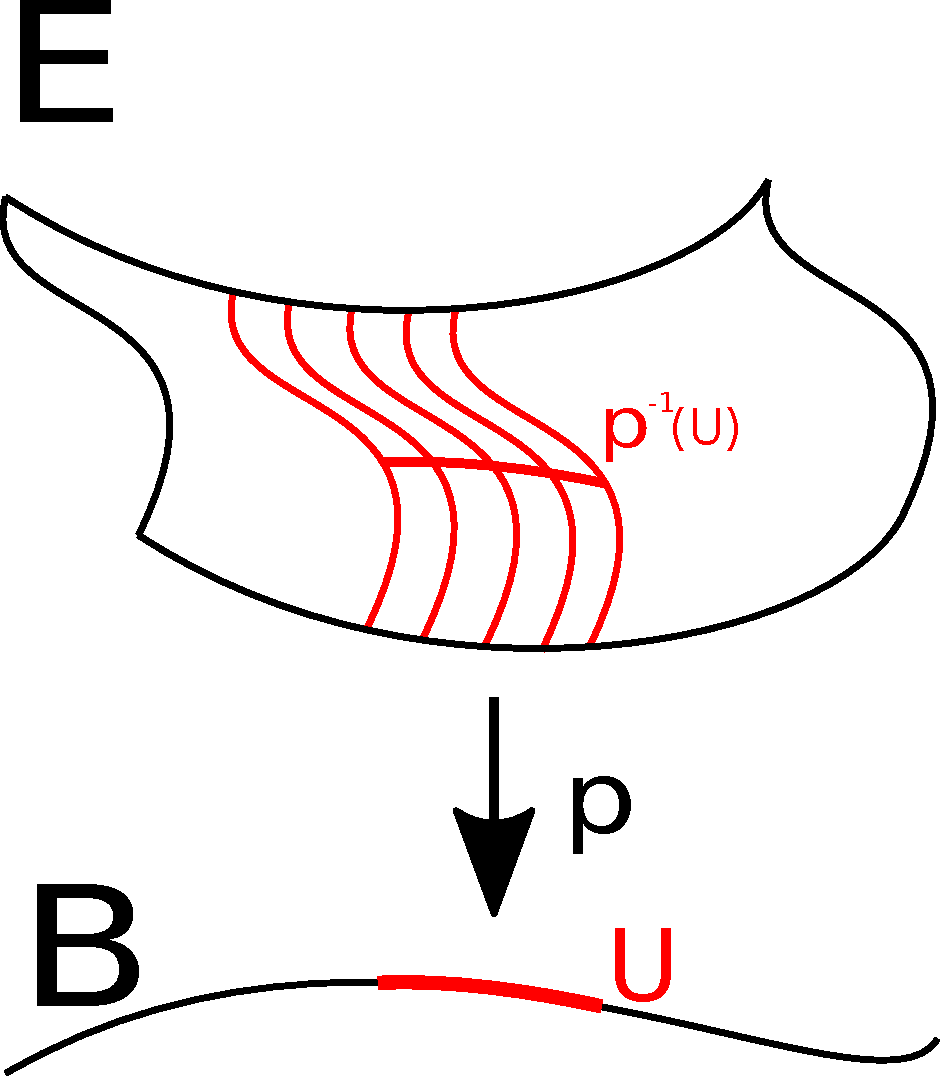
\includegraphics[scale=0.3]{fibrado.pdf}
	\caption{Ilustração da trivialidade local de um fibrado vetorial.}
\end{figure}

\par Note que, todo fibrado vetorial $\xi=(E,p,B)$ admite uma seção $s:B\to E$, chamada de seção nula\index{seção!nula}, que é definida por $s(b)=0\in p^{-1}(b)$.

\begin{defi}\label{fv_iso}
	Dizemos que dois $\R^{n}-$fibrados vetoriais $\xi=(E,p,B)$ e $\xi'=(E',q,B)$ são isomorfos\index{isomorfismo}, denotado por $\xi\cong\xi'$, se existir um homeomorfismo $h:E\to E'$ tal que $q\circ h=p$ e $h|_{p^{-1}(b)}:p^{-1}(b)\to q^{-1}(b)$ seja um isomorfismo vetorial\index{isomorfismo!vetorial} para todo $b\in B$.
\end{defi}

\par Agora, lembremos como definir em específico os fibrados vetoriais tangente e normal de uma variedade suave e de um mergulho suave, respectivamente.

\par Considere $M^{m}$ uma variedade suave $m-$dimensional e defina $TM=\ds\bigcup_{b\in M}\{b\}\times T_{b}M$, lembrando que $T_{b}M$ é o espaço tangente de $M$ em $b$.

\par Então, $\tau(M)=(TM,p_{1},M)$ será um $\R^{m}-$fibrado vetorial com fibra $p_{1}^{-1}(b)=\{b\}\times T_{b}M$ sobre $b\in M$.

\begin{defi}\label{defi_fvt}
	\par $\tau(M)$ é chamado de fibrado vetorial tangente\index{fibrado!vetorial!tangente} da variedade suave\index{variedade!suave} $M$.
\end{defi}

\par Por outro lado, recordemos que uma imersão\index{imersão} $i:N^{n}\to M^{n+k}$ é uma aplicação entre variedades suaves de modo que sua diferencial $d_{b}i:T_{b}N\to T_{i(b)}M$ é uma transformação linear injetiva, para todo $b\in N$.

\par Neste contexto, podemos garantir que $d_{b}i(T_{b}N)$ é um subespaço linear de $T_{i(b)}M$. Assim, fica bem definido o conjunto $E(i)=\{ (b,v)\in N\times T_{i(b)}M \ : \ v\in [d_{b}i(T_{b}N)]^{\perp}\subset T_{i(b)}M \}$.

\par Logo, $\nu(i)=(E(i),p_{1},N)$ será um $\R^{k}-$fibrado vetorial sendo $p_{1}^{-1}(b)=\{b\}\times [d_{b}i(T_{b}N)]^{\perp}$ sua fibra sobre $b\in M$.

\begin{defi}\label{defi_fvn}
	$\nu(i)$ é chamado de fibrado vetorial normal\index{fibrado!vetorial!normal} da imersão $i:N\to M$.
\end{defi}

\par Note que o fibrado vetorial normal pode ser definido para um mergulho suave\index{mergulho!suave}, uma vez que todo mergulho suave é um mergulho topológico\index{mergulho!topológico} e uma imersão\index{imersão}.

\par Encerrando os tópicos sobre fibrados vetoriais, vejamos a seguinte relação entre os fibrados vetoriais tangente e normal de um mergulho suave, entre variedades suaves\index{variedade!suave}, cuja prova pode ser encontrada em (\cite{milnor_1}, Corolários 3.4 e 3.5, p. 30-31).

\begin{teo}\label{dualidade_whitney_vet}
	Se $i:N^{n}\to M^{n+k}$ é um mergulho suave entre variedades suaves, então:
	$$ \tau(N)\oplus\nu(i)\cong i^{*}(\tau(M)) $$
\end{teo}



% ------------------------------------------------------------------------------------------
% ------------------------------------------------------------------------------------------
% ------------------------------------------------------------------------------------------



\section{Fibração e Fibração de Pares}\label{secao_fib_pares}

\

\par Definiremos nesta seção o conceito de fibração de pares\index{fibração!de pares}, também desenvolvido por Fadell em \cite{fadell_1}, que pode ser considerado como uma fibração\index{fibração} cujo espaço total é um par de espaços topológicos.

\par A definição de fibração de pares será necessária quando definirmos os fibrados generalizados\index{fibrado!generalizado} na próxima seção. Utilizaremos as propriedades desenvolvidas nesta seção como um passo intermediário nas demonstrações dos resultados que envolverão fibrados generalizados.

\par Com exceção do exemplo \ref{pf_fv}, todos o resultados que serão apresentados no decorrer desta seção podem ser encontrados, sem muito detalhes, em \cite{fadell_1} e \cite{brown}.

\begin{defi}\label{PLH}
	Dizemos que uma aplicação $p:E\to B$ admite a propriedade do levantamento de homotopia\index{levantamento de homotopia} (PLH) sobre um espaço topológico $X$ se para quaisquer aplicações $h:X\to E$ e $H:X\times I\to B$, tais que $H(\_,0)=p\circ h$, existir $\wt{H}:X\times I\to E$ contínua tal que $\wt{H}(\_,0)=h$ e $p\circ\wt{H}=H$. Deste modo, temos o seguinte diagrama comutativo:
	
	$$ \xymatrix @C=0.5cm {
		X\times \{ 0 \} \ar[rrr]^-{h} \ar@{^(->}[dd] &&& E \ar[dd]^-{p} \\
		&&& \\
		X\times I \ar[rrr]^-{H} \ar[rrruu]^-{\wt{H}} &&& B
	}$$
\end{defi}

\begin{defi}
	Uma aplicação sobrejetiva $p:E\to B$ é dita uma fibração\index{fibração} se $p$ admite a PLH sobre qualquer espaço topológico $X$.
	
	\par Neste contexto, chamamos a terna $\mathcal{F}=(E,p,B)$ de fibração sobre um espaço base $B$, com espaço total $E$ e fibra $F=p^{-1}(b)$ sobre $b\in B$. Diremos que uma aplicação $s:B\to E$ é uma seção\index{seção} de $\mathcal{F}$ se $p\circ s=1$.
\end{defi}

\begin{defi}{\bf (Fibração de Pares)}\label{defi_par-fib}
	Sejam $p:E\to B$ uma aplicação sobrejetiva e $E_{0}\subset E$. Chamamos $(\mathcal{F},\mathcal{F}_{0})=(E,E_{0},p,B)$ de fibração de pares\index{fibração!de pares} se para qualquer espaço topológico $X$ e quaisquer aplicações $h:X\to E$ e $H:X\times I\to B$, tais que $H(\_,0)=p\circ h$, existir $\wt{H}:X\times I\to E$ contínua tal que $\wt{H}(\_,0)=h$, $p\circ\wt{H}=H$ e se $x_{0}\in X$ é tal que $h(x_{0})\in E_{0}$, então $\wt{H}(x_{0},\_)\in E_{0}$.
	
	\par Neste contexto, diremos que $(\mathcal{F},\mathcal{F}_{0})$ é uma fibração de pares sobre um espaço base $B$, com espaço total $(E,E_{0})$ e fibra $(F,F_{0})=(p^{-1}(b),p^{-1}(b)\cap E_{0})$ sobre $b\in B$.
	
	\par Diremos também que uma aplicação $s:B\to E$ é uma seção\index{seção} de $(\mathcal{F},\mathcal{F}_{0})$ se $p\circ s=1$.
\end{defi}

\par Note que, a definição \ref{defi_par-fib} garante que $\mathcal{F}=(E,p,B)$ e $\mathcal{F}_{0}=(E_{0},p_{0}=p_{|E_{0}},B)$ são fibrações.

\par Historicamente, o conceito de fibração coincide com o conceito de "fiber space\index{fiber space}" dado por Hurewicz em (\cite{hurewicz}, Seção 1, p. 956), como mostrado também em (\cite{hurewicz}, Seção 2, p. 957). Assim, o conceito de fibração de pares coincide com o chamado "fibered pair\index{fibered pair}" dado por Fadell em (\cite{fadell_1}, Definição 2.3, p. 489), como mostrado em (\cite{brown}, Lema 1.4, p. 183).

\par Como exemplo mais simples de uma fibração de pares, temos o já esperado:

\begin{ex}\label{pf_trivial}
	Considerando $B$ um espaço topológico arbitrário, então obtemos que $(\varepsilon_{B}^{n},\varepsilon_{B}^{n,0})=(B\times\R^{n},B\times(\R^{n}-\{ 0 \}),p_{1},B)$ é uma fibração de pares com fibra homeomorfa a $(\R^{n},\R^{n}-\{ 0 \})$.
\end{ex}
\begin{proof}
	
	\
	
	\par Inicialmente, considere $X$ um espaço topológico qualquer e aplicações $h:X\to B\times\R^{n}$ e $H:X\times I\to B$ de modo a obter o seguinte diagrama comutativo:
	
	$$\xymatrix @C=0.5cm {
		X\times\{ 0 \} \ar[rrr]^-{h} \ar@{^(->}[dd] &&& B\times\R^{n} \ar[dd]^-{p_{1}} \\
		&&& \\
		X\times I \ar[rrr]^-{H} &&& B
	}$$
	
	\par Como $h=(h_{1},h_{2})$, defina $\wt{H}:X\times I\to B\times\R^{n}$ por $\wt{H}(x,t)=(H(x,t),h_{2}(x))$. É claro que $\wt{H}$ é contínua, $p_{1}\circ\wt{H}=H$ e $\wt{H}(\_,0)=h$, pois $H(\_,0)=h_{1}$. Ainda, se $x_{0}\in X$ é tal que $h(x_{0})\in B\times (\R^{n}-\{ 0 \})$, então $h_{2}(x_{0})\in \R^{n}-\{ 0 \}$, e assim, $\wt{H}(x_{0},\_)\in B\times(\R^{n}-\{ 0 \})$.
	
	\par Por fim, dada $(F,F_{0})$ a fibra de $(\mathcal{F},\mathcal{F}_{0})$ sobre $b\in B$ qualquer, então: \newline
	
	$\begin{array}{rl}
		F \ = & p_{1}^{-1}(b) \\
		= & \{ b \}\times\R^{n} \\
		\approx & \R^{n}
	\end{array}$
	
	\
	
	\
	
	$\begin{array}{rl}
		F_{0} \ = & p_{1}^{-1}(b)\bigcap [B\times(\R^{n}-\{ 0 \})] \\
		= & [\{ b \}\times\R^{n}]\bigcap [B\times(\R^{n}-\{ 0 \})] \\
		= & \{ b \}\times(\R^{n}-\{ 0 \}) \\
		\approx & \R^{n}-\{ 0 \}
	\end{array}$ \newline
	
	\par Logo, $(\varepsilon_{B}^{n},\varepsilon_{B}^{n,0})$ é, de fato, uma fibração de pares.
	
\end{proof}

\par Note que o exemplo \ref{pf_trivial} também continua válido se trocarmos $\R^{n}$ por um espaço topológico $F$ qualquer e $\R^{n}-\{ 0 \}$ por um subespaço $F_{0}\subset F$ qualquer. Entretanto, a fibra seria, neste caso, homeomorfa ao par $(F,F_{0})$.

\par A seguir, veremos um modo alternativo de construir fibrações de pares, cuja prova pode ser encontrada em (\cite{allaud}, Teorema 2.5, p.241).

\begin{teo}\label{teo_hurewicz}
	Sejam $p:E\to B$ uma aplicação sobrejetiva com $B$ paracompacto e pares $(F,F_{0})$ e $(E,E_{0})$. Se existir uma cobertura aberta $\mathcal{U}$ de $B$ tal que, para todo $U\in\mathcal{U}$, existir um homeomorfismo $h_{U}:(U\times F,U\times F_{0})\to (p^{-1}(U),p^{-1}(U)\cap E_{0})$ de modo que $p\circ h_{U}=p_{1}$, então $(E,E_{0},p,B)$ será uma fibração de pares.
\end{teo}

\par O teorema \ref{teo_hurewicz} pode ser considerado a versão do teorema da Uniformização de Hurewicz\index{teorema!da Uniformização de Hurewicz}\footnote{Para mais detalhes sobre o teorema da Uniformização de Hurewicz, ver \cite{hurewicz}.} para fibrações de pares.

\par Deste modo, podemos obter o seguinte:

\begin{ex}\label{pf_fv}
	Todo $\R^{n}-$fibrado vetorial\index{fibrado!vetorial}, sobre uma base paracompacta, pode ser associado a uma fibração de pares\index{fibração!de pares}, cuja fibra será homeomorfa ao par $(\R^{n},\R^{n}-\{ 0 \})$.
\end{ex}
\begin{proof}
	
	\
	
	\par Primeiramente, considere $\xi=(E,p,B)$ um $\R^{n}-$fibrado vetorial sobre $B$ paracompacto. Pela definição \ref{fv_defi}, sabemos que existe uma cobertura aberta $\mathcal{U}$ de $B$ tal que, para todo $U\in\mathcal{U}$, existe um homeomorfismo $h_{U}:U\times\R^{n}\to p^{-1}(U)$ satisfazendo $p\circ h_{U}=p_{1}$.
	
	\par Assim, denotando por $s:B\to E$ a seção nula\index{seção!nula} de $\xi$ e $E_{0}=E-s(B)$, fica evidente que podemos considerar $h_{U}:(U\times\R^{n},U\times(\R^{n}-\{ 0 \}))\to (p^{-1}(U),p^{-1}(U)\cap E_{0})$ como um homeomorfismo de pares.
	
	\par Portanto, segue do teorema \ref{teo_hurewicz} que $(\xi,\xi_{0})=(E,E_{0},p,B)$ será uma fibração de pares.
	
\end{proof}

\par Agora, como última parte desta seção, vejamos como construir algumas fibrações de pares a partir de outras.

\begin{lem}\label{pf_restricao}
	Sejam $(\mathcal{F},\mathcal{F}_{0})=(E,E_{0},p,B)$ uma fibração de pares e $U\subset B$ qualquer. Então, $(\mathcal{F},\mathcal{F}_{0})_{|U}=(p^{-1}(U),p^{-1}(U)\cap E_{0},p_{|p^{-1}(U)},U)$ será uma fibração de pares\index{fibração!de pares} com fibra igual a fibra de $(\mathcal{F},\mathcal{F}_{0})$.
\end{lem}
\begin{proof}
	
	\
	
	\par Primeiramente, denotemos $q=p_{|p^{-1}(U)}$ e consideremos $X$ um espaço topológico qualquer e aplicações $h:X\to p^{-1}(U)$ e $H:X\times I\to U$ de modo que o seguinte diagrama comute:
	
	$$ \xymatrix @C=0.5cm {
		X\times\{ 0 \} \ar[rrr]^-{h} \ar@{^(->}[dd] &&& p^{-1}(U) \ar[dd]^-{q} \\
		&&& \\
		X\times I \ar[rrr]^-{H} &&& U 
	}$$
	
	\par Como $Im(H)\subset U\subset B$ e $(\mathcal{F},\mathcal{F}_{0})$ é uma fibração de pares, então existe uma aplicação $\wt{H}:X\times I\to E$ tal que $p\circ\wt{H}=H$ e $\wt{H}(\_,0)=h$. Por outro lado, $Im(p\circ\wt{H})=Im(H)\subset U$, e assim, $Im(\wt{H})\subset p^{-1}(U)$.
	
	\par Por outro lado, se $x_{0}\in X$ é tal que $h(x_{0})\in E_{0}$, então $\wt{H}(x_{0},\_)\in E_{0}$, ou seja, se $h(x_{0})\in p^{-1}(U)\cap E_{0}$, então $\wt{H}(x_{0},\_)\in p^{-1}(U)\cap E_{0}$.
	
	\par Por fim, sendo $(F',F'_{0})$ e $(F,F_{0})$ as fibras de $(\mathcal{F},\mathcal{F}_{0})_{|U}$ e $(\mathcal{F},\mathcal{F}_{0})$, respectivamente, sobre o mesmo $b\in U$, temos que: \newline
	
	$\begin{array}{rl}
		F' \ = & q^{-1}(b) \\
		= & p^{-1}(b)\cap p^{-1}(U) \\
		= & p^{-1}(b) \\
		= & F
	\end{array}$
	
	\
	
	\
	
	$\begin{array}{rl}
		F'_{0} \ = & q^{-1}(b)\bigcap [p^{-1}(U)\cap E_{0}] \\
		= & p^{-1}(b)\bigcap [p^{-1}(U)\cap E_{0}] \\
		= & p^{-1}(b)\cap E_{0} \\
		= & F_{0}
	\end{array}$ \newline
	
	\par Portanto, $(\mathcal{F},\mathcal{F}_{0})_{|U}$ será uma fibração de pares.
	
\end{proof}

\begin{lem}\label{pf_pullback}
	Sejam $(\mathcal{F},\mathcal{F}_{0})=(E,E_{0},p,B)$ uma fibração de pares e $f:B'\to B$ uma aplicação. Então, $f^{*}(\mathcal{F},\mathcal{F}_{0})=(f^{*}E,f^{*}E_{0},p_{1},B')$ também será uma fibração de pares\index{fibração!de pares} e com fibra homeomorfa a fibra de $(\mathcal{F},\mathcal{F}_{0})$, em que:
	
	\begin{enumerate}
		\item $f^{*}E=\{ (b',e)\in B'\times E \ : \ f(b')=p(e) \}$
		\item $f^{*}E_{0}=\{ (b',e)\in f^{*}E \ : \ e\in E_{0} \}$
	\end{enumerate}
	
\end{lem}
\begin{proof}
	
	\
	
	\par Inicialmente, considere $X$ um espaço topológico qualquer e aplicações $h:X\to f^{*}E$ e $H:X\times I\to B'$ tais que o seguinte diagrama comuta:
	
	$$\xymatrix @C=0.5cm {
		X\times\{ 0 \} \ar[rrr]^-{h} \ar@{^(->}[dd] &&& f^{*}E \ar[rrr]^-{p_{2}} \ar[dd]^-{p_{1}} &&& E \ar[dd]^-{p} \\
		&&& &&& \\
		X\times I \ar[rrr]^-{H} &&& B' \ar[rrr]^-{f} &&& B
	}$$
	
	\par Denotando $g=p_{2}\circ h:X\to E$ e $G=f\circ H:X\times I\to B$, como o diagrama acima é comutativo e $(\mathcal{F},\mathcal{F}_{0})$ é uma fibração de pares, então existe $\wt{G}:X\times I\to E$ de modo que $p\circ\wt{G}=G$, $\wt{G}(\_,0)=g$ e se $x_{0}\in X$ é tal que $g(x_{0})\in E_{0}$, então $\wt{G}(x_{0},\_)\in E_{0}$.
	
	\par Por outro lado, é claro que $\wt{H}=(H,\wt{G}):X\times I\to f^{*}E$ está bem definido, pois $f\circ H=G=p\circ\wt{G}$. Ainda, $p_{1}\circ\wt{H}=H$ e $\wt{H}(\_,0)=h$, uma vez que $H(\_,0)=p_{1}\circ h$ e $\wt{G}(\_,0)=p_{2}\circ h$.
	
	\par Assim, se $x_{0}\in X$ é tal que $h(x_{0})\in f^{*}E_{0}$, então, $g(x_{0})=p_{2}\circ h(x_{0})\in E_{0}$, e consequentemente, $\wt{G}(x_{0},\_)\in E_{0}$. Logo, $\wt{H}(x_{0},\_)\in f^{*}E_{0}$.
	
	\par Por fim, se $(F',F'_{0})$ e $(F,F_{0})$ são fibras de $f^{*}(\mathcal{F},\mathcal{F}_{0})$ e $(\mathcal{F},\mathcal{F}_{0})$ sobre $b'_{0}\in B'$ e $f(b'_{0})\in B$, respectivamente, então: \newline
	
	$\begin{array}{rl}
		F' \ = & p_{1}^{-1}(b'_{0}) \\
		= & \{ (b',e)\in f^{*}E \ : \ b'=p_{1}(b',e)=b'_{0} \} \\
		= & \{ (b'_{0},e)\in B'\times E \ : \ f(b'_{0})=p(e) \} \\
		= & \{ (b'_{0},e)\in B'\times E \ : \ e\in p^{-1}(f(b'_{0})) \} \\
		= & \{ b'_{0} \}\times p^{-1}(f(b'_{0})) \\
		= & \{ b'_{0} \}\times F \\
		\approx & F
	\end{array}$
	
	\
	
	\
	
	$\begin{array}{rl}
		F'_{0} \ = & p_{1}^{-1}(b'_{0})\cap f^{*}E_{0} \\
		= & (\{ b'_{0} \}\times F)\bigcap f^{*}E_{0} \\
		= & \{ b'_{0} \}\times (F\cap E_{0}) \\
		= & \{ b'_{0} \}\times F_{0} \\
		\approx & F_{0}
	\end{array}$ \newline
	
	\par Logo, $f^{*}(\mathcal{F},\mathcal{F}_{0})$ é, de fato, uma fibração de pares.
	
\end{proof}

\begin{lem}\label{pf_produto}
	Sejam $(\mathcal{F},\mathcal{F}_{0})=(E,E_{0},p,B)$ e $(\mathcal{F'},\mathcal{F'}_{0})=(E',E'_{0},q,B')$ duas fibrações de pares. Então, $(\mathcal{F},\mathcal{F}_{0})\times(\mathcal{F'},\mathcal{F'}_{0})=(E'',E''_{0},r,B'')$ será uma fibração de pares\index{fibração!de pares} com fibra igual ao produto das fibras de $(\mathcal{F},\mathcal{F}_{0})$ e $(\mathcal{F'},\mathcal{F'}_{0})$, em que:
	
	\begin{enumerate}
		\item $E''=E\times E'$
		\item $E''_{0}=(E\times E'_{0})\cup (E_{0}\times E')$
		\item $r=p\times q$
	\end{enumerate}
	
\end{lem}
\begin{proof}
	
	\
	
	\par Inicialmente, considere $X$ um espaço topológico qualquer e aplicações $h:X\to E''$ e $H:X\times I\to B''$ de modo que o seguinte diagrama comute:
	
	$$\xymatrix @C=0.5cm {
		X\times\{ 0 \} \ar[rrr]^-{h} \ar@{^(->}[dd] &&& E'' \ar[dd]^-{r} \\
		&&& &&& \\
		X\times I \ar[rrr]^-{H} &&& B'' 
	}$$
	
	\par Como $h=(h_{1},h_{2})$, $H=(H_{1},H_{2})$ e $H(\_,0)=r\circ h$, então $H_{1}(\_,0)=p\circ h_{1}$ e $H_{2}(\_,0)=q\circ h_{2}$. Sendo $(\mathcal{F},\mathcal{F}_{0})$ e $(\mathcal{F'},\mathcal{F'}_{0})$ fibrações de pares, então existem aplicações $\wt{H_{1}}:X\times I\to E$ e $\wt{H_{2}}:X\times I\to E'$ tais que $p\circ\wt{H_{1}}=H_{1}$, $q\circ\wt{H_{2}}=H_{2}$, $\wt{H_{1}}(\_,0)=h_{1}$, $\wt{H_{2}}(\_,0)=h_{2}$ e se $x_{0}\in X$ é tal que $h_{1}(x_{0})\in E_{0}$, então $\wt{H_{1}}(x_{0},\_)\in E_{0}$. Ainda, se $x_{0}\in X$ é tal que $h_{2}(x_{0})\in E'_{0}$, então $\wt{H_{2}}(x_{0},\_)\in E'_{0}$.
	
	\par Deste modo, definindo $\wt{H}=(\wt{H_{1}},\wt{H_{2}}):X\times I\to E''$, é claro que $\wt{H}(\_,0)=h$ e $r\circ\wt{H}=H$. Ainda, se $x_{0}\in X$ é tal que $h(x_{0})\in E''_{0}$, então $h_{1}(x_{0})\in E_{0}$ ou $h_{2}(x_{0})\in E'_{0}$. Assim, $\wt{H_{1}}(x_{0},\_)\in E_{0}$ ou $\wt{H_{2}}(x_{0},\_)\in E'_{0}$, isto é, $\wt{H}(x_{0},\_)\in E''_{0}$.
	
	\par Por fim, considere, respectivamente, $(F,F_{0})$, $(F',F'_{0})$ e $(F'',F''_{0})$ fibras de $(\mathcal{F},\mathcal{F}_{0})$, $(\mathcal{F'},\mathcal{F'}_{0})$ e $(\mathcal{F},\mathcal{F}_{0})\times (\mathcal{F'},\mathcal{F'}_{0})$ sobre $b\in B$, $b'\in B'$ e $(b,b')\in B''$. Então: \newline
	
	$\begin{array}{rl}
		F'' \ = & r^{-1}(b,b') \\
		= & p^{-1}(b)\times q^{-1}(b') \\
		= & F\times F'
	\end{array}$
	
	\
	
	\
	
	$\begin{array}{rl}
		F''_{0} \ = & r^{-1}(b,b')\cap E''_{0} \\
		= & (F\times F')\bigcap [(E\times E'_{0})\cup (E_{0}\times E')] \\
		= & [(F\times F')\cap (E\times E'_{0})]\bigcup [(F\times F')\cap (E_{0}\times E')] \\
		= & [F\times (F'\cap E'_{0})]\bigcup [(F\cap E_{0})\times F'] \\
		= & (F\times F'_{0})\cup (F_{0}\times F')
	\end{array}$ \newline
	
	\par Portanto, $(\mathcal{F},\mathcal{F}_{0})\times (\mathcal{F'},\mathcal{F'}_{0})$ será uma fibração de pares.
	
\end{proof}



% ------------------------------------------------------------------------------------------
% ------------------------------------------------------------------------------------------
% ------------------------------------------------------------------------------------------



\section{Fibrado Generalizado}\label{secao_fib_gener}

\

\par Nesta seção, apresentaremos a ferramenta desenvolvida por Fadell em \cite{fadell_1} que possibilita generalizarmos fibrados vetoriais tangente\index{fibrado!vetorial!tangente} e normal\index{fibrado!vetorial!normal} de variedades suaves\index{variedade!suave} para variedades topológicas\index{variedade!topológica}. Tal ferramenta foi denominada de fibrado generalizado.

\par Com exceção dos exemplos \ref{fht_sobre_ponto} e \ref{fht_fv}, dos lemas \ref{iso_homot} e \ref{iso_homot_2} e das proposições \ref{iso_fv_fht}, \ref{iso_homeo}, \ref{fht_tang_cart} e \ref{iso_merg_lf_2}, todos os outros resultados foram retirados de \cite{fadell_1}, entretanto, apresentaremos aqui demonstrações mais detalhadas destes.

\begin{defi}{\bf (Fibrado Generalizado)}\label{defi_fib_gen}
	Chamamos uma fibração de pares\index{fibração!de pares} $(\mathcal{F},\mathcal{F}_{0})=(E,E_{0},p,B)$ de $\R^{n}-$fibrado generalizado\index{fibrado!generalizado} quando:
	
	\begin{enumerate}
		\item existir uma seção\index{seção} $s:B\to E$ de $(\mathcal{F},\mathcal{F}_{0})$ que realiza $E_{0}$, isto é, $E_{0}=E-s(B)$
		\item toda fibra $(F,F_{0})$ de $(\mathcal{F},\mathcal{F}_{0})$ é tal que $(F,F_{0})\sim (\R^{n},\R^{n}-\{ 0 \})$
	\end{enumerate}
\end{defi}

\begin{ex}\label{fht_trivial}
	A fibração de pares $(\varepsilon^{n}_{B},\varepsilon^{n,0}_{B})$ é um $\R^{n}-$fibrado generalizado.
\end{ex}
\begin{proof}
	
	\
	
	\par Devido ao exemplo \ref{pf_trivial}, já sabemos que $(\varepsilon^{n}_{B},\varepsilon^{n,0}_{B})$ é uma fibração de pares com fibra homeomorfa ao par $(\R^{n},\R^{n}-\{ 0 \})$. Deste modo, basta definir uma seção de $(\varepsilon^{n}_{B},\varepsilon^{n,0}_{B})$ que realize $B\times(\R^{n}-\{ 0 \})$.
	
	\par Note que $s:B\to B\times\R^{n}$ definida por $s(b)=(b,0)$ é a seção procurada.
	
	\par Logo, $(\varepsilon^{n}_{B},\varepsilon^{n,0}_{B})$ é um $\R^{n}-$fibrado geberalizado.
	
\end{proof}

\begin{lem}\label{fht_restricao}
	Se $(\mathcal{F},\mathcal{F}_{0})$ é um $\R^{n}-$fibrado generalizado\index{fibrado!generalizado} sobre $B$, então $(\mathcal{F},\mathcal{F}_{0})_{|U}$ também será um $\R^{n}-$fibrado generalizado para todo $U\subset B$.
\end{lem}
\begin{proof}
	
	\
	
	\par Devido ao lema \ref{pf_restricao}, já sabemos que se $(\mathcal{F},\mathcal{F}_{0})$ é uma fibração de pares\index{fibração!de pares}, então dado $U\subset B$ arbitrário, $(\mathcal{F},\mathcal{F}_{0})_{|U}$ também será uma fibração de pares com fibra igual a fibra de $(\mathcal{F},\mathcal{F}_{0})$. Deste modo, ao denotarmos $(\mathcal{F},\mathcal{F}_{0})=(E,E_{0},p,B)$ e $(\mathcal{F},\mathcal{F}_{0})_{|U}=(p^{-1}(U),p^{-1}(U)\cap E_{0},p_{|p^{-1}(U)},U)$, basta encontrar uma seção\index{seção} de $(\mathcal{F},\mathcal{F}_{0})_{|U}$ que realize $p^{-1}(U)\cap E_{0}$.
	
	\par Para tanto, como $(\mathcal{F},\mathcal{F}_{0})$ é um $\R^{n}-$fibrado generalizado, então existe $s:B\to E$ seção de $(\mathcal{F},\mathcal{F}_{0})$ que realiza $E_{0}$. Agora, defina $s'=s_{|U}:U\to p^{-1}(U)$. É claro que $Im(s')\subset p^{-1}(U)$, pois $p\circ s(U)=U$. Ainda, temos: \newline
	
	$\begin{array}{rl}
		p^{-1}(U)\cap E_{0} \ = & p^{-1}(U)\bigcap [E-s(B)] \\
		= & [p^{-1}(U)\cap E]-[p^{-1}(U)\cap s(B)] \\
		= & p^{-1}(U)-s(U) \\
		= & p^{-1}(U)-s'(U)
	\end{array}$ \newline
	
	\par Portanto, $(\mathcal{F},\mathcal{F}_{0})_{|U}$ também será um $\R^{n}-$fibrado generalizado, para todo $U\subset B$.
	
\end{proof}

\par Seguindo as notações do lema \ref{fht_restricao}, sendo $(\mathcal{F},\mathcal{F}_{0})$ um $\R^{n}-$fibrado generalizado, chamamos $(\mathcal{F},\mathcal{F}_{0})_{|U}$ de $\R^{n}-$fibrado generalizado restrição\index{fibrado!generalizado!restrição} de $(\mathcal{F},\mathcal{F}_{0})$ a $U\subset B$.

\begin{defi}
	Sejam $(\mathcal{F},\mathcal{F}_{0})=(E,E_{0},p,B)$ e $(\mathcal{F'},\mathcal{F'}_{0})=(E',E'_{0},q,B)$ $\R^{n}-$fibrados generalizados sobre a mesma base. Chamamos $\phi:(\mathcal{F},\mathcal{F}_{0})\to (\mathcal{F'},\mathcal{F'}_{0})$ de aplicação fibrada\index{aplicação!fibrada} se $\phi:(E,E_{0})\to (E',E'_{0})$ for uma aplicação que preserva fibra, isto é, $q\circ\phi=p$.
\end{defi}

\begin{defi}\label{defi_iso_homot}
	Dizemos que dois $\R^{n}-$fibrados generalizados $(\mathcal{F},\mathcal{F}_{0})=(E,E_{0},p,B)$ e $(\mathcal{F'},\mathcal{F'}_{0})=(E',E'_{0},q,B)$, sobre a mesma base, são homotopicamente isomorfos se existirem aplicações fibradas $\phi:(\mathcal{F},\mathcal{F}_{0})\rightleftarrows (\mathcal{F'},\mathcal{F'}_{0}):\psi$ e homotopias $H:(E,E_{0})\times I\to (E,E_{0})$ e $G:(E',E'_{0})\times I\to (E',E'_{0})$ tais que: \newline
	
	$\begin{array}{lcccl}
		1. \ H(\_,0)=\psi\circ\phi            & & & & 4. \ G(\_,0)=\phi\circ\psi \\
		2. \ H(\_,1)=1                        & & & & 5. \ G(\_,1)=1 \\
		3. \ p\circ H(\_,t)=p, \forall t\in I & & & & 6. \ q\circ G(\_,t)=q, \forall t\in I
	\end{array}$ \newline
	
	\par O isomorfismo homotópico\index{isomorfismo!homotópico}, acima definido, será denotado por $(\mathcal{F},\mathcal{F}_{0})\sim_{f} (\mathcal{F'},\mathcal{F'}_{0})$.
\end{defi}

\par A noção de isomorfismo homotópico, dada na definição acima, coincide com o conceito de "fiber homotopy equivalence\index{fiber homotopy equivalence}" dada por Fadell em (\cite{fadell_1}, Definição 2.4, p. 489).

\begin{defi}
	Chamamos um $\R^{n}-$fibrado generalizado $(\mathcal{F},\mathcal{F}_{0})$, sobre $B$, de localmente trivial\index{localmente trivial} se existir uma cobertura aberta $\mathcal{U}$ de $B$ tal que $(\mathcal{F},\mathcal{F}_{0})_{|U}\sim_{f} (\varepsilon^{n}_{U},\varepsilon^{n,0}_{U})$, para qualquer $U\in\mathcal{U}$. Em particular, $(\mathcal{F},\mathcal{F}_{0})$ será chamado de $\R^{n}-$fibrado generalizado trivial\index{fibrado!generalizado!trivial} se $(\mathcal{F},\mathcal{F}_{0})\sim_{f} (\varepsilon^{n}_{B},\varepsilon^{n,0}_{B})$.
\end{defi}

\begin{ex}\label{fht_sobre_ponto}
	Todo $\R^{n}-$fibrado generalizado sobre um ponto é trivial.
\end{ex}
\begin{proof}
	
	\
	
	\par Denotemos por $(\mathcal{F},\mathcal{F}_{0})=(E,E_{0},p,\{ * \})$ um $\R^{n}-$fibrado generalizado cujo espaço base é constituído de apenas um ponto.
	
	\par Assim, é claro que $(E,E_{0})=(p^{-1}(*),p^{-1}(*)\cap E_{0})\sim (\R^{n},\R^{n}-\{0 \})$, isto é, existem aplicações $\phi:(E,E_{0})\rightleftarrows (\R^{n},\R^{n}-\{ 0 \}):\psi$ e homotopias $H:(E,E_{0})\times I\to (E,E_{0})$ e $G:(\R^{n},\R^{n}-\{0 \})\times I\to (\R^{n},\R^{n}-\{0 \})$ tais que $H(\_,0)=\psi\circ\phi$, $H(\_,1)=1$, $G(\_,0)=\phi\circ\psi$ e $G(\_,1)=1$.
	
	\par Deste modo, ficam bem definidas as seguintes aplicações fibradas\index{aplicação!fibrada} e homotopias:
	
	\begin{enumerate}
		\item $\overline{\phi}:(E,E_{0})\rightleftarrows (\{ * \}\times\R^{n},\{ * \}\times\R^{n}-\{0 \}):\overline{\psi}$ \\
		$ \overline{\phi}(e)=(*,\phi(e)) $ \\
		$ \overline{\psi}(*,x)=\psi(x) $
		\item $\overline{H}:(E,E_{0})\times I\to (E,E_{0})$ \\
		$ \overline{H}(e,t)=H(e,t) $
		\item $\overline{G}:(\{ * \}\times\R^{n},\{ * \}\times\R^{n}-\{0 \})\times I \to (\{ * \}\times\R^{n},\{ * \}\times\R^{n}-\{0 \})$ \\
		$ \overline{G}((*,x),t)=(*,G(x,t)) $
	\end{enumerate}
	
	\par É claro que $\overline{H}(\_,1)=1$, $\overline{G}(\_,1)=1$, $p\circ\overline{H}(\_,t)=p$ e $p_{1}\circ\overline{G}(\_,t)=p_{1}$ para qualquer $t\in I$. Ainda: \newline 
	
	$\begin{array}{rl}
		\forall e\in E, \ \overline{H}(e,0) \ = & H(e,0) \\
		= & \psi\circ\phi(e) \\
		= & \overline{\psi}(*,\phi(e)) \\
		= & \overline{\psi}\circ\overline{\phi}(e)
	\end{array}$
	
	$\begin{array}{rl}
		\forall x\in \R^{n}, \ \overline{G}((*,x),0) \ = & (*,G(x,0)) \\
		= & (*,\phi\circ\psi(x)) \\
		= & \overline{\phi}(\psi(x)) \\
		= & \overline{\phi}\circ\overline{\psi}(*,x)
	\end{array}$ \newline 
	
	\par Logo, $(\mathcal{F},\mathcal{F}_{0})\sim_{f}(\varepsilon^{n}_{\{ * \}},\varepsilon^{n,0}_{\{ * \}})$.
	
\end{proof}

\par Sobre condições específicas, o isomorfismo homotópico\index{isomorfismo!homotópico} pode ser garantido, de modo mais simples, como no seguinte:

\begin{lem}\label{iso_homot}
	Sejam $(\mathcal{F},\mathcal{F}_{0})$ e $(\mathcal{F'},\mathcal{F'}_{0})$ dois $\R^{n}-$fibrados generalizados, sobre a mesma base. Se $\phi:(\mathcal{F},\mathcal{F}_{0})\to (\mathcal{F'},\mathcal{F'}_{0})$ for uma aplicação fibrada\index{aplicação!fibrada} tal que $\phi$ é um homeomorfismo, então $(\mathcal{F},\mathcal{F}_{0})\sim_{f} (\mathcal{F'},\mathcal{F'}_{0})$.
\end{lem}
\begin{proof}
	
	\
	
	\par Inicialmente, como $\phi$ um homeomorfismo e $q\circ\phi=p$, então $p\circ\phi^{-1}=q$, ou seja, $\phi^{-1}:(\mathcal{F},\mathcal{F}_{0})\to (\mathcal{F'},\mathcal{F'}_{0})$ também é uma aplicação fibrada.
	
	\par Assim, fica evidente que $(\mathcal{F},\mathcal{F}_{0})\sim_{f} (\mathcal{F},\mathcal{F}_{0})$, uma vez que é suficiente definir as homotopias triviais para que as condições sobre isomorfismo homotópico sejam satisfeitas.
	
\end{proof}

\par Deste modo, utilizando o lema \ref{iso_homot} e a construção do exemplo \ref{pf_fv}, obtemos o seguinte:

\begin{ex}\label{fht_fv}
	Se $\xi$ é um $\R^{n}-$fibrado vetorial\index{fibrado!vetorial} sobre uma base paracompacta, então sua fibração de pares\index{fibração!de pares} associada $(\xi,\xi_{0})$ será um $\R^{n}-$fibrado generalizado\index{fibrado!generalizado} localmente trivial\index{localmente trivial}.
\end{ex}

\par Com isso, podemos considerar que a noção de fibrados generalizados generaliza o conceito de fibrados vetoriais. Assim, é esperado que a estrutura de isomorfismo entre fibrados vetoriais seja mantida quando passada para isomorfismo homotópico\index{isomorfismo!homotópico}, como na seguinte:

\begin{prop}\label{iso_fv_fht}
	Sejam $\xi$ e $\eta$ dois $\R^{n}-$fibrados vetoriais\index{fibrado!vetorial} isomorfos\index{isomorfismo} sobre uma mesma base paracompacta. Então, seus respectivos $\R^{n}-$fibrados generalizados associados $(\xi,\xi_{0})$ e $(\eta,\eta_{0})$ são homotopicamente isomorfos.
\end{prop}
\begin{proof}
	
	\
	
	\par Primeiramente, denotemos $\xi=(E,p,B)\cong\eta=(E',q,B)$. Deste modo, segue da definição \ref{fv_iso} que existe um homeomorfismo $h:E\to E'$ tal que $q\circ h=p$ e $h_{|F}:F\to F'$ é um isomorfismo vetorial\index{isomorfismo!vetorial}, para quaisquer fibras $F$ e $F'$ de $\xi$ e $\eta$, respectivamente, sobre o mesmo $b\in B$.
	
	\par Sendo $s:B\to E$ e $s':B\to E'$ as seções nulas\index{seção!nula} de $\xi$ e $\eta$, respectivamente, consideremos $E_{0}=E-s(B)$ e $E'_{0}=E'-s'(B)$. Se mostrarmos que $h(E_{0})\subset E'_{0}$, teremos que $h:(E,E_{0})\to (E',E'_{0})$ será um homeomorfismo e uma aplicação fibrada\index{aplicação!fibrada}, e assim, o lema \ref{iso_homot} garantirá que $(\xi,\xi_{0})\sim_{f} (\eta,\eta_{0})$.
	
	\par Para tanto, note que: \newline
	
	$\begin{array}{rl}
		e\in E_{0} \Longrightarrow \ & e\in F=p^{-1}(p(e))\cong\R^{n} \ e \ e\neq 0 \\
		\Longrightarrow & h(e)\in F'=q^{-1}(p(e))\cong\R^{n} \ e \ h(e)\neq 0 \\
		\Longrightarrow & h(e)\in E'_{0}
	\end{array}$ \newline
	
	\par Portanto, concluímos que $(\xi,\xi_{0})\sim_{f} (\eta,\eta_{0})$.
	
\end{proof}

\begin{lem}\label{fht_pullback}
	Se $(\mathcal{F},\mathcal{F}_{0})$ é um $\R^{n}-$fibrado generalizado\index{fibrado!generalizado!trivial} sobre $B$ e $f:B'\to B$ é uma aplicação qualquer, então $f^{*}(\mathcal{F},\mathcal{F}_{0})$ também será um $\R^{n}-$fibrado generalizado. Em particular, se $(\mathcal{F},\mathcal{F}_{0})$ for trivial, então $f^{*}(\mathcal{F},\mathcal{F}_{0})$ também será trivial.
\end{lem}
\begin{proof}
	
	\
	
	\par Devido ao lema \ref{pf_pullback}, já sabemos que se $(\mathcal{F},\mathcal{F}_{0})$ é uma fibração de pares\index{fibração!de pares}, então $f^{*}(\mathcal{F},\mathcal{F}_{0})$ será uma fibração de pares com fibra homeomorfa a fibra de $(\mathcal{F},\mathcal{F}_{0})$. Com isso, denotando $(\mathcal{F},\mathcal{F}_{0})=(E,E_{0},p,B)$ e $f^{*}(\mathcal{F},\mathcal{F}_{0})=(f^{*}E,f^{*}E_{0},p_{1},B')$, basta mostrar que existe uma seção\index{seção} de $f^{*}(\mathcal{F},\mathcal{F}_{0})$ que realiza $f^{*}E_{0}$.
	
	\par Para tanto, como $(\mathcal{F},\mathcal{F}_{0})$ é um $\R^{n}-$fibrado generalizado, então existe uma seção $s:B\to E$ de $(\mathcal{F},\mathcal{F}_{0})$ que realiza $E_{0}$. Deste modo, fica bem definida a seção $s':B'\to f^{*}E$, de $f^{*}(\mathcal{F},\mathcal{F}_{0})$, dada por $s'(b')=(b',s(f(b')))$. Por fim: \newline
	
	$\begin{array}{rl}
		f^{*}E_{0} \ = & [B'\times E_{0}]\bigcap f^{*}E \\
		= & [B'\times (E-s(B))]\bigcap f^{*}E \\
		= & [(B'\times E)-(B'\times s(B))]\bigcap f^{*}E \\
		= & [(B'\times E)\cap f^{*}E]-[(B'\times s(B))\cap f^{*}E] \\
		= & f^{*}E - \{ (b',s(b))\in B'\times s(B) \ : \ f(b')=p(s(b))=b \} \\
		= & f^{*}E - [B'\times s(f(B'))] \\
		= & f^{*}E - s'(B')
	\end{array}$ \newline
	
	\par Logo, $f^{*}(\mathcal{F},\mathcal{F}_{0})$ será um $\R^{n}-$fibrado generalizado.
	
	\par Agora, resta mostrar que se $(\mathcal{F},\mathcal{F}_{0})\sim_{f}(\varepsilon_{B}^{n},\varepsilon_{B}^{n,0})$, então $f^{*}(\mathcal{F},\mathcal{F}_{0})\sim_{f}(\varepsilon_{B'}^{n},\varepsilon_{B'}^{n,0})$. Assim, suponha que existam as seguintes aplicações fibradas\index{aplicação!fibrada} e homotopias satisfazendo as relações a seguir: 
	
	\begin{enumerate}
		\item $\phi:(E,E_{0})\rightleftarrows(B\times \R^{n},B\times (\R^{n}-\{ 0 \})):\psi$
		\item $H:(E,E_{0})\times I\to (E,E_{0})$
		\item $G:(B\times\R^{n},B\times(\R^{n}-\{ 0 \}))\times I\to (B\times\R^{n},B\times(\R^{n}-\{ 0 \}))$
		\item $\phi$, $\psi$, $H$ e $G$ satisfazem:
		$\begin{array}{lcccl}
			H(\_,0)=\psi\circ\phi            & & & & G(\_,0)=\phi\circ\psi \\
			H(\_,1)=1                        & & & & G(\_,1)=1 \\
			p\circ H(\_,t)=p, \forall t\in I & & & & p_{1}\circ G(\_,t)=p_{1}, \forall t\in I
		\end{array}$	
	\end{enumerate}
	
	\par Com isso, ficam bem definidas as seguintes aplicações fibradas e homotopias:
	
	\begin{enumerate}
		\item $\overline{\phi}:(f^{*}E,f^{*}E_{0})\rightleftarrows (B'\times \R^{n},B'\times (\R^{n}-\{ 0 \})):\overline{\psi}$ \\
		$ \overline{\phi}(b',e)=(b',p_{2}\circ\phi(e)) $ \\
		$ \overline{\psi}(b',x)=(b',\psi(f(b'),x)) $
		\item $\overline{H}:(f^{*}E,f^{*}E_{0})\times I\to (f^{*}E,f^{*}E_{0})$ \\
		$ \overline{H}((b',e),t)=(b',H(e,t)) $
		\item $\overline{G}:(B'\times \R^{n},B'\times (\R^{n}-\{ 0 \}))\times I\to (B'\times \R^{n},B'\times (\R^{n}-\{ 0 \}))$ \\
		$ \overline{G}((b',x),t)=(b',p_{2}\circ G((f(b'),x),t)) $
	\end{enumerate}
	
	\par Mostremos que $\overline{\phi}$, $\overline{\psi}$, $\overline{H}$ e $\overline{G}$ satisfazem as condições da definição \ref{defi_iso_homot}. De fato:
	
	\begin{enumerate}
		\item é claro que $p_{1}\circ\overline{H}((\_,\_),t)=p_{1}$ e $p_{1}\circ\overline{G}((\_,\_),t)=p_{1}$ para todo $t\in I$
		\item também é claro que $\overline{H}((\_,\_),1)=1$ e $\overline{G}((\_,\_),1)=1$
		\item $\begin{array}{rl}
			\forall (b',e)\in f^{*}E, \ \overline{H}((b',e),0) \ = & (b',H(e,0)) \\
			= & (b',\psi\circ\phi(e)) \\
			= & (b',\psi(p_{1}\circ\phi(e),p_{2}\circ\phi(e))) \\
			= & (b',\psi(p(e),p_{2}\circ\phi(e))) \\
			= & (b',\psi(f(b'),p_{2}\circ\phi(e))) \\
			= & \overline{\psi}(b',p_{2}\circ\phi(e)) \\
			= & \overline{\psi}\circ\overline{\phi}(b',e)
		\end{array}$
		\item $\begin{array}{rl}
			\forall (b',x)\in B'\times\R^{n}, \ \overline{G}((b',x),0) \ = & (b',p_{2}\circ G((f(b'),x),0)) \\
			= & (b',p_{2}\circ\phi\circ\psi(f(b'),x)) \\
			= & \overline{\phi}(b',\psi(f(b'),x)) \\
			= & \overline{\phi}\circ\overline{\psi}(b',x)
		\end{array}$
	\end{enumerate}
	
	\par Portanto, $f^{*}(\mathcal{F},\mathcal{F}_{0})\sim_{f}(\varepsilon_{B'}^{n},\varepsilon_{B'}^{n,0})$.
	
\end{proof}

\par Seguindo as notações do lema \ref{fht_pullback}, dado $(\mathcal{F},\mathcal{F}_{0})$ um $\R^{n}-$fibrado generalizado, chamamos $f^{*}(\mathcal{F},\mathcal{F}_{0})$ de $\R^{n}-$fibrado generalizado pullback\index{fibrado!generalizado!pullback} de $(\mathcal{F},\mathcal{F}_{0})$ pela aplicação f.

\par Agora, vejamos alguns exemplos envolvendo fibrados generalizados pullbacks.

\begin{ex}\label{fht_pullback_ex1}
	\par Sejam $(\mathcal{F},\mathcal{F}_{0})$ e $(\mathcal{F'},\mathcal{F'}_{0})$ dois $\R^{n}-$fibrados generalizados, sobre a mesma base $B$, tais que $(\mathcal{F},\mathcal{F}_{0})\sim_{f} (\mathcal{F'},\mathcal{F'}_{0})$. Então, sendo $1:B\to B$ a aplicação identidade, temos $(\mathcal{F},\mathcal{F}_{0})\sim_{f} 1^{*}(\mathcal{F'},\mathcal{F'}_{0})$.
\end{ex}
\begin{proof}
	
	\
	
	\par Inicialmente, denotemos $(\mathcal{F},\mathcal{F}_{0})=(E,E_{0},p,B)$ e $(\mathcal{F'},\mathcal{F'}_{0})=(E',E'_{0},q,B)$. Como $(\mathcal{F},\mathcal{F}_{0})\sim_{f} (\mathcal{F'},\mathcal{F'}_{0})$, então existem as seguintes aplicações fibradas e homotopias satisfazendo as relações a seguir:
	
	\begin{enumerate}
		\item $\phi:(E,E_{0})\rightleftarrows (E',E'_{0}):\psi$
		\item $H:(E,E_{0})\times I\to (E,E_{0})$
		\item $G:(E',E'_{0})\times I\to (E',E'_{0})$
		\item $\phi$, $\psi$ $H$ e $G$ são tais que: $\begin{array}{lcccl}
			\ H(\_,0)=\psi\circ\phi            & & & & \ G(\_,0)=\phi\circ\psi \\
			\ H(\_,1)=1                        & & & & \ G(\_,1)=1 \\
			\ p\circ H(\_,t)=p, \forall t\in I & & & & \ q\circ G(\_,t)=q, \forall t\in I
		\end{array}$
	\end{enumerate}
	
	\par Recordando que o $\R^{n}-$fibrado generalizado pullback\index{fibrado!generalizado!pullback} $1^{*}(\mathcal{F'},\mathcal{F'}_{0})=(1^{*}E',1^{*}E'_{0},p_{1},B)$ é tal que $1^{*}E'=\{ (b,e')\in B\times E' \ : \ b=q(e') \}$ e $1^{*}E'_{0}=\{ (b,e')\in 1^{*}E' \ : \ e'\in E'_{0} \}$, então ficam bem definidas as seguintes aplicações fibradas\index{aplicação!fibrada} e homotopias:
	
	\begin{enumerate}
		\item $\overline{\phi}:(E,E_{0})\rightleftarrows (1^{*}E',1^{*}E'_{0}):\overline{\psi}$ \\
		$\overline{\phi}(e)=(p(e),\phi(e))$ \\
		$\overline{\psi}(b,e')=\psi(e')$
		\item $\overline{H}:(E,E_{0})\times I\to (E,E_{0})$ \\
		$\overline{H}(e,t)=H(e,t)$
		\item $\overline{G}:(1^{*}E',1^{*}E'_{0})\times I\to (1^{*}E',1^{*}E'_{0})$ \\
		$\overline{G}((b,e'),t)=(b,G(e',t))$
	\end{enumerate}
	
	\par Com isso, é claro que $\overline{H}(e,1)=e$, para todo $e\in E$, e $p\circ\overline{H}(\_,t)=p$, para todo $t\in I$, pois $H$ tem essas propriedades. Analogamente, $\overline{G}((b,e'),1)=(b,e')$, para todo $(b,e')\in 1^{*}E'$, e $p_{1}\circ\overline{G}(\_,t)=p_{1}$, para todo $t\in I$. Ainda, temos que: \newline
	
	$\begin{array}{rl}
		\forall e\in E, \ \overline{H}(e,0) \ = & H(e,0) \\
		= & \psi\circ\phi(e) \\
		= & \overline{\psi}(p(e),\phi(e)) \\
		= & \overline{\psi}\circ\overline{\phi}(e)
	\end{array}$
	
	\
	
	\
	
	$\begin{array}{rl}
		\forall (b,e')\in 1^{*}E', \ \overline{G}((b,e'),0) \ = & (b,G(e',0)) \\
		= & (b,\phi\circ\psi(e')) \\
		= & (q(e'),\phi\circ\psi(e')) \\
		= & (p\circ\psi(e'),\phi\circ\psi(e')) \\
		= & \overline{\phi}(\psi(e')) \\
		= & \overline{\phi}\circ\overline{\psi}(b,e')
	\end{array}$ \newline
	
	\par Portanto, $(\mathcal{F},\mathcal{F}_{0})\sim_{f} 1^{*}(\mathcal{F'},\mathcal{F'}_{0})$.
	
\end{proof}

\begin{ex}\label{fht_pullback_ex2}
	Sejam $B$ um espaço topológico, $b_{0}\in B$ qualquer e $c:B\to \{ b_{0} \}$ a aplicação constante. Então, $(\varepsilon^{n}_{B},\varepsilon^{n,0}_{B})\sim_{f} c^{*}(\varepsilon^{n}_{\{ b_{0} \}},\varepsilon^{n,0}_{\{ b_{0} \}})$.
\end{ex}
\begin{proof}
	
	\
	
	\par Lembremos que $c^{*}(\varepsilon^{n}_{\{ b_{0} \}},\varepsilon^{n,0}_{\{ b_{0} \}})=(c^{*}(\{ b_{0} \}\times\R^{n}),c^{*}[\{ b_{0} \}\times (\R^{n}-\{ 0 \})],p_{1},B)$ é o $\R^{n}-$fibrado generalizado pullback\index{fibrado!generalizado!pullback} tal que: \newline
	
	$\begin{array}{rl}
		c^{*}(\{ b_{0} \}\times\R^{n})= & \{ (b,(b_{0},x))\in B\times(\{ b_{0} \}\times\R^{n}) \ : \ b_{0}=c(b)=p_{1}(b_{0},x)=b_{0} \} \\
		= & B\times \{ b_{0} \}\times\R^{n}
	\end{array}$
	
	\
	
	\
	
	$c^{*}[\{ b_{0} \}\times (\R^{n}-\{ 0 \})]=B\times\{ b_{0} \}\times(\R^{n}-\{ 0 \})$ \newline
	
	\par Assim, $\phi:(B\times\R^{n},B\times(\R^{n}-\{ 0 \}))\rightleftarrows (B\times\{ b_{0} \}\times\R^{n},B\times\{ b_{0} \}\times(\R^{n}-\{ 0 \})):\psi$, dadas por $\phi(b,x)=(b,b_{0},x)$ e $\psi(b,b_{0},x)=(b,x)$, respectivamente, são aplicações fibradas\index{aplicação!fibrada} bem definidas, sendo $\phi$ um homeomorfismo com inversa $\psi$.
	
	\par Logo, segue do lema \ref{iso_homot} que $(\varepsilon^{n}_{B},\varepsilon^{n,0}_{B})\sim_{f} c^{*}(\varepsilon^{n}_{\{ b_{0} \}},\varepsilon^{n,0}_{\{ b_{0} \}})$.
	
\end{proof}

\par O próximo resultado é uma versão mais geral do lema \ref{iso_homot}, envolvendo, agora, fibrados generalizados sobre diferentes bases.

\begin{lem}\label{iso_homot_2}
	Seja $(\mathcal{F},\mathcal{F}_{0})=(E,E_{0},p,B)$ um $\R^{n}-$fibrado generalizado. Se $h:B'\to B$ e $H:(E',E'_{0})\to (E,E_{0})$ forem homeomorfismos, então $(\mathcal{F'},\mathcal{F'}_{0})=(E',E'_{0},h^{-1}\circ p\circ H,B')$ também será um $\R^{n}-$fibrado generalizado. Ainda, $(\mathcal{F'},\mathcal{F'}_{0})\sim_{f} h^{*}(\mathcal{F},\mathcal{F}_{0})$.
\end{lem}
\begin{proof}
	
	\
	
	\par Denotando $q=h^{-1}\circ p\circ H$, provemos, inicialmente, que $(\mathcal{F'},\mathcal{F'}_{0})$ é uma fibração de pares\index{fibração!de pares}. Para tanto, considere $X$ um espaço topológico qualquer e aplicações $f:X\to E'$ e $F:X\times I\to B'$ tais que $F(\_,0)=q\circ f$.
	
	\par Ao definirmos as aplicações $g=H\circ f:X\to E$ e $G=h\circ F:X\times I\to B$, é claro que: \newline 
	
	$\begin{array}{rl}
		G(\_,0) \ = & h\circ F(\_,0) \\
		= & h\circ q\circ f \\
		= & p\circ H\circ f \\
		= & p\circ g
	\end{array}$ \newline 
	
	\par Deste modo, obtemos o seguinte diagrama comutativo:
	
	$$ \xymatrix @C=0.5cm {
		X\times \{ 0 \} \ar[rrr]^-{f} \ar@{^(->}[dd] \ar@/^0.6cm/[rrrrrr]^-{g} &&& E' \ar[rrr]^-{H} \ar[dd]^{q} &&& E \ar[dd]^-{p} \\
		&&& &&& \\
		X\times I \ar[rrr]^-{F} \ar@/_0.6cm/[rrrrrr]_-{G} &&& B' \ar[rrr]^-{h} &&& B
	} $$
	
	\par Sendo $(\mathcal{F},\mathcal{F}_{0})$ uma fibração de pares, sabemos que existe uma aplicação $\wt{G}:X\times I\to E$ tal que $\wt{G}(\_,0)=g$, $p\circ \wt{G}=G$ e se $g(x)\in E_{0}$, então $\wt{G}(x,\_)\in E_{0}$. Assim, definindo a aplicação $\wt{F}=H^{-1}\circ \wt{G}:X\times I\to E'$, temos: \newline 
	
	$\begin{array}{rl}
		\wt{F}(\_,0) \ = & H^{-1}\circ \wt{G}(\_,0) \\
		= & H^{-1}\circ g \\
		= & H^{-1}\circ H\circ f \\
		= & f
	\end{array}$
	
	\
	
	\
	
	$\begin{array}{rl}
		q\circ \wt{F} \ = & h^{-1}\circ p\circ H\circ H^{-1}\circ \wt{G} \\
		= & h^{-1}\circ p\circ \wt{G} \\
		= & h^{-1}\circ G \\
		= & h^{-1}\circ h\circ F \\
		= & F
	\end{array}$
	
	\
	
	\
	
	$\begin{array}{rl}
		f(x)\in E'_{0} \Longrightarrow \ & g(x)=H\circ f(x)\in E_{0} \\
		\Longrightarrow & \wt{G}(x,\_)\in E_{0} \\
		\Longrightarrow & \wt{F}(x,\_)=H^{-1}\circ \wt{G}(x,\_)\in E'_{0}
	\end{array}$ \newline 
	
	\par Com isso, concluímos que $(\mathcal{F'},\mathcal{F'}_{0})$ é, de fato, uma fibração de pares.
	
	\par Agora, provemos que $(\mathcal{F'},\mathcal{F'}_{0})$ é um $\R^{n}-$fibrado generalizado\index{fibrado!generalizado}. Como existe $s:B\to E$ seção\index{seção} de $(\mathcal{F},\mathcal{F}_{0})$ que realiza $E_{0}$, então, ao definirmos $s':H^{-1}\circ s\circ h:B'\to E'$, teremos que: \newline 
	
	$\begin{array}{rl}
		q\circ s' \ = & h^{-1}\circ p\circ H\circ H^{-1}\circ s\circ h \\
		= & h^{-1}\circ p\circ s\circ h \\
		= & h^{-1}\circ h \\
		= & 1
	\end{array}$
	
	\
	
	\
	
	$\begin{array}{rl}
		E'-s'(B') \ = & H^{-1}(E)-H^{-1}(s(h(B'))) \\
		= & H^{-1}(E-s(B)) \\
		= & H^{-1}(E_{0}) \\
		= & E'_{0}
	\end{array}$ \newline
	
	\par Assim, $s'$ é uma seção de $(\mathcal{F'},\mathcal{F'}_{0})$ que realiza $E'_{0}$. Por outro lado, como toda fibra de $(\mathcal{F},\mathcal{F}_{0})$ tem o mesmo tipo de homotopia que $(\R^{n},\R^{n}-\{ 0 \})$, então, para todo $b'\in B'$, temos: \newline
	
	$\begin{array}{rl}
		q^{-1}(b')=       & H^{-1}(p^{-1}(h(b'))) \\
		\approx & p^{-1}(h(b')) \\
		\sim    & \R^{n}
	\end{array}$
	
	\
	
	\
	
	$\begin{array}{rl}
		q^{-1}(b')\cap E'_{0}=       & H^{-1}(p^{-1}(h(b')))\bigcap H^{-1}(E_{0}) \\
		=       & H^{-1}(p^{-1}(h(b'))\cap E_{0}) \\
		\approx & p^{-1}(h(b'))\cap E_{0} \\
		\sim    & \R^{n}-\{ 0 \}
	\end{array}$ \newline 
	
	\par Deste modo, $(\mathcal{F'},\mathcal{F'}_{0})$ será um $\R^{n}-$fibrado generalizado.
	
	\par Por fim, mostremos que $(\mathcal{F'},\mathcal{F'}_{0})\sim_{f} h^{*}(\mathcal{F},\mathcal{F}_{0})$. Para tanto, lembremos que $h^{*}(\mathcal{F},\mathcal{F}_{0})=(h^{*}E,h^{*}E_{0},p_{1},B')$, em que:
	$$ h^{*}E=\{ (b',e)\in B'\times E \ : \ h(b')=p(e) \} $$
	$$ h^{*}E_{0}=\{ (b',e)\in h^{*}E \ : \ e\in E_{0} \} $$
	
	\par Considerando $\phi:(E',E'_{0})\rightleftarrows (h^{*}E,h^{*}E_{0}):\psi$ dadas por $\phi(e')=(q(e'),H(e'))$ e $\psi(b',e)=H^{-1}(e)$, respectivamente, conluímos que $\phi$ e $\psi$ são aplicações fibradas\index{aplicação!fibrada} bem definidas sendo $\phi$ um homeomorfismo com inversa $\psi$.
	
	\par Portanto, segue do lema \ref{iso_homot} que $(\mathcal{F'},\mathcal{F'}_{0})\sim_{f} h^{*}(\mathcal{F},\mathcal{F}_{0})$.
	
\end{proof}

\begin{lem}\label{fht_produto}
	Se $(\mathcal{F},\mathcal{F}_{0})$ é um $\R^{n}-$fibrado generalizado e $(\mathcal{F'},\mathcal{F'}_{0})$ é um $\R^{m}-$fibrado generalizado, então $(\mathcal{F},\mathcal{F}_{0})\times(\mathcal{F'},\mathcal{F'}_{0})$ será um $\R^{n+m}-$fibrado generalizado. Em particular, se $(\mathcal{F},\mathcal{F}_{0})$ e $(\mathcal{F'},\mathcal{F'}_{0})$ forem triviais, então $(\mathcal{F},\mathcal{F}_{0})\times (\mathcal{F'},\mathcal{F'}_{0})$ também será trivial\index{fibrado!generalizado!trivial}.
\end{lem}
\begin{proof}
	
	\
	
	\par Primeiramente, denotemos $(\mathcal{F},\mathcal{F}_{0})=(E,E_{0},p,B)$ e $(\mathcal{F'},\mathcal{F'}_{0})=(E',E'_{0},q,B')$ e considere $(\mathcal{F},\mathcal{F}_{0})\times(\mathcal{F'},\mathcal{F'}_{0})=(E'',E''_{0},r,B'')$, em que $E''=E\times E'$, $E''_{0}=(E\times E'_{0})\cup (E_{0}\times E')$, $r=p\times q$ e $B''=B\times B'$.
	
	\par Devido ao lema \ref{pf_produto}, já sabemos que se $(\mathcal{F},\mathcal{F}_{0})$ e $(\mathcal{F'},\mathcal{F'}_{0})$ são fibrações de pares\index{fibração!de pares}, então $(\mathcal{F},\mathcal{F}_{0})\times(\mathcal{F'},\mathcal{F'}_{0})$  será uma fibração de pares com fibra igual ao produto das fibras de $(\mathcal{F},\mathcal{F}_{0})$ e $(\mathcal{F'},\mathcal{F'}_{0})$. Assim, resta mostrar que existe uma seção\index{seção} de $(\mathcal{F},\mathcal{F}_{0})\times(\mathcal{F'},\mathcal{F'}_{0})$ que realiza $E''_{0}$.
	
	\par Para tanto, como $(\mathcal{F},\mathcal{F}_{0})$ e $(\mathcal{F'},\mathcal{F'}_{0})$ são fibrados generalizados, então existem seções $s:B\to E$ e $s':B'\to E'$ de $(\mathcal{F},\mathcal{F}_{0})$ e $(\mathcal{F'},\mathcal{F'}_{0})$ que realizam $E_{0}$ e $E'_{0}$, respectivamente. Deste modo, temos que $s'':B''\to E''$, definida por $s''(b,b')=(s(b),s'(b'))$, é uma seção de $(\mathcal{F},\mathcal{F}_{0})\times(\mathcal{F'},\mathcal{F'}_{0})$ tal que: \newline
	
	$\begin{array}{rl}
		E''_{0} \ = & (E\times E'_{0})\bigcup (E_{0}\times E') \\
		= & [E\times (E'-s'(B'))]\bigcup [(E-s(B))\times E'] \\
		= & [(E\times E')-(E\times s'(B'))] \bigcup [(E\times E')-(s(B)\times E')] \\
		= & (E\times E')-[(E\times s'(B'))\bigcap (s(B)\times E')] \\
		= & E''-(s(B)\times s'(B')) \\
		= & E''-s''(B'')
	\end{array}$ \newline
	
	\par Assim, $(\mathcal{F},\mathcal{F}_{0})\times(\mathcal{F'},\mathcal{F'}_{0})$ será um $\R^{n+m}-$fibrado generalizado\index{fibrado!generalizado}.
	
	\par Agora, resta mostrar que se $(\mathcal{F},\mathcal{F}_{0})\sim_{f}(\varepsilon^{n}_{B},\varepsilon^{n,0}_{B})$ e $(\mathcal{F'},\mathcal{F'}_{0})\sim_{f}(\varepsilon^{m}_{B'},\varepsilon^{m,0}_{B'})$, então $(\mathcal{F},\mathcal{F}_{0})\times(\mathcal{F'},\mathcal{F'}_{0})\sim_{f}(\varepsilon^{n+m}_{B''},\varepsilon^{n+m,0}_{B''})$. Para tanto, suponha que existam as seguintes aplicações fibradas\index{aplicação!fibrada} e homotopias satisfazendo as relações a seguir:
	
	\begin{enumerate}
		\item $\phi:(E,E_{0})\rightleftarrows(B\times \R^{n},B\times (\R^{n}-\{ 0 \})):\psi$
		\item $H:(E,E_{0})\times I\to (E,E_{0})$
		\item $G:(B\times\R^{n},B\times(\R^{n}-\{ 0 \}))\times I\to (B\times\R^{n},B\times(\R^{n}-\{ 0 \}))$
		\item $\phi$, $\psi$, $H$ e $G$ são tais que: $\begin{array}{lcccl}
			H(\_,0)=\psi\circ\phi            & & & & G(\_,0)=\phi\circ\psi \\
			H(\_,1)=1                        & & & & G(\_,1)=1 \\
			p\circ H(\_,t)=p, \forall t\in I & & & & p_{1}\circ G(\_,t)=p_{1}, \forall t\in I
		\end{array}$
	\end{enumerate}
	
	\par Ainda, suponha que também existam as seguintes aplicações fibradas e homotopias satisfazendo também as relações a seguir:
	
	\begin{enumerate}
		\item $\phi':(E',E'_{0})\rightleftarrows(B'\times \R^{m},B'\times (\R^{m}-\{ 0 \})):\psi'$
		\item $H':(E',E'_{0})\times I\to (E',E'_{0})$
		\item $G':(B'\times\R^{m},B'\times(\R^{m}-\{ 0 \}))\times I\to (B'\times\R^{m},B'\times(\R^{m}-\{ 0 \}))$
		\item $\phi'$, $\psi'$, $H'$ e $G'$ são tais que: $\begin{array}{lcccl}
			H'(\_,0)=\psi'\circ\phi'            & & & & G'(\_,0)=\phi'\circ\psi' \\
			H'(\_,1)=1                          & & & & G'(\_,1)=1 \\
			q\circ H'(\_,t)=q, \forall t\in I   & & & & p_{1}\circ G'(\_,t)=p_{1}, \forall t\in I
		\end{array}$
	\end{enumerate}
	
	\par Com isso, ficam bem definidas as seguintes aplicações fibradas e homotopias:
	
	\begin{enumerate}
		\item $\phi'':(E'',E''_{0})\rightleftarrows (B''\times \R^{n+m},B''\times (\R^{n+m}-\{ 0 \})):\psi''$ \\
		$ \phi''(e,e')=((p(e),q(e')),(p_{2}\circ\phi(e),p_{2}\circ\phi'(e'))) $ \\
		$ \psi''((b,b'),(x,x'))=(\psi(b,x),\psi'(b',x')) $
		\item $H'':(E'',E''_{0})\times I\to (E'',E''_{0})$ \\
		$ H''((e,e'),t)=(H(e,t),H'(e',t)) $
		\item $G'':(B''\times \R^{n+m},B''\times (\R^{n+m}-\{ 0 \}))\times I\to (B''\times \R^{n+m},B''\times (\R^{n+m}-\{ 0 \}))$ \\
		$ G''(((b,b'),(x,x')),t)=((b,b'),(p_{2}\circ G((b,x),t),p_{2}\circ G'((b',x'),t))) $
	\end{enumerate}
	
	\par Mostremos que $\phi''$, $\psi''$, $H''$ e $G''$ satisfazem as condições da definição \ref{defi_iso_homot}. De fato:
	
	\begin{enumerate}
		\item é claro que $r\circ H''((\_,\_),t)=r$ e $(p_{1}\times p_{2})\circ G''((\_,\_),t)=p_{1}\times p_{2}$, para qualquer $t\in I$
		\item também é claro que $H''((\_,\_),1)=1$ e $G''((\_,\_),1)=1$
		\item $\begin{array}{rl}
			\forall (e,e')\in E'', H''((e,e'),0) \ = & (H(e,0),H'(e',0)) \\
			= & (\psi\circ\phi(e),\psi'\circ\phi'(e')) \\
			= & (\psi(p_{1}\circ\phi(e),p_{2}\circ\phi(e)),\psi'(p_{1}\circ\phi'(e'),p_{2}\circ\phi'(e'))) \\
			= & (\psi(p(e),p_{2}\circ\phi(e)),\psi'(q(e'),p_{2}\circ\phi'(e'))) \\
			= & \psi''((p(e),q(e')),(p_{2}\circ\phi(e),p_{2}\circ\phi'(e'))) \\
			= & \psi''\circ\phi''(e,e')
		\end{array}$
		\item $\begin{array}{rl}
			\forall ((b,b'),(x,x'))\in B''\times\R^{n+m}, & \\
			G''(((b,b'),(x,x')),0) \ = & ((b,b'),(p_{2}\circ G((b,x),0),p_{2}\circ G'((b',x'),0))) \\
			= & ((b,b'),(p_{2}\circ\phi\circ\psi(b,x),p_{2}\circ\phi'\circ\psi'(b',x'))) \\
			= & \phi''(\psi(b,x),\psi'(b',x')) \\
			= & \phi''\circ\psi''((b,b'),(x,x'))
		\end{array}$
	\end{enumerate}
	
	\par Logo, $(\mathcal{F},\mathcal{F}_{0})\times(\mathcal{F'},\mathcal{F'}_{0})\sim_{f}(\varepsilon^{n+m}_{B''},\varepsilon^{n+m,0}_{B''})$.
	
\end{proof}

\par Seguindo as notações do lema \ref{fht_produto}, dado $(\mathcal{F},\mathcal{F}_{0})$ um $\R^{n}-$fibrado generalizado e $(\mathcal{F'},\mathcal{F'}_{0})$ um $\R^{m}-$fibrado generalizado, chamamos $(\mathcal{F},\mathcal{F}_{0})\times(\mathcal{F'},\mathcal{F'}_{0})$ de $\R^{n+m}-$fibrado generalizado produto\index{fibrado!generalizado!produto} de $(\mathcal{F},\mathcal{F}_{0})$ e $(\mathcal{F'},\mathcal{F'}_{0})$.

\begin{defi}{\bf (Soma de Whitney)}
	Sejam $(\mathcal{F},\mathcal{F}_{0})$ um $\R^{n}-$fibrado generalizado e $(\mathcal{F'},\mathcal{F'}_{0})$ um $\R^{m}-$fibrado generalizado, ambos sobre a mesma base $B$, e $d:B\to B\times B$ a aplicação diagonal\index{aplicação!diagonal}. Definimos a soma de Whitney\index{fibrado!generalizado!soma de Whitney} entre $(\mathcal{F},\mathcal{F}_{0})$ e $(\mathcal{F'},\mathcal{F'}_{0})$ como sendo o seguinte $\R^{n+m}-$fibrado generalizado:
	$$ (\mathcal{F},\mathcal{F}_{0})\oplus(\mathcal{F'},\mathcal{F'}_{0})=d^{*}[(\mathcal{F},\mathcal{F}_{0})\times(\mathcal{F'},\mathcal{F'}_{0})] $$
\end{defi}



% ------------------------------------------------------------------------------------------
% ------------------------------------------------------------------------------------------
% ------------------------------------------------------------------------------------------



\subsection{Fibrado Tangente de uma Variedade Topológica}\label{secao_fht_tang}

\

\par Nesta subseção, mostraremos que o conceito de fibrado generalizado permite generalizar a noção de fibrado vetorial tangente\index{fibrado!vetorial!tangente} de variedades suaves\index{variedade!suave} para variedades topológicas\index{variedade!topológica}.

\par Para tanto, considere $M^{m}$ uma variedade topológica e defina:

\begin{itemize}
	\item $T_{0}M=\{ \omega\in M^{I} \ : \ \omega(t)=\omega(0) \Leftrightarrow t=0 \}$
	\item $TM=T_{0}M \bigcup \{ \omega\in M^{I} \ : \ \omega(t)=\omega(0), \ \forall t\in I \}$
	\item $p:TM\to M$, dada por $p(\omega)=\omega(0)$
\end{itemize}

\par Então, obtemos a seguinte:

\begin{prop}\label{fgt}
	Seja $M^{m}$ uma variedade topológica. Então, o par $(\tau M,\tau_{0}M)=(TM,T_{0}M,p,M)$ será um $\R^{m}-$fibrado generalizado\index{fibrado!generalizado} localmente trivial\index{localmente trivial}.
\end{prop}

\par A prova da proposição acima pode ser encontrada em (\cite{fadell_1}, Proposição 3.8, p. 493).

\begin{obs}\label{obs_varied_bordo}
	Vale ressaltar que a construção feita por Fadell em \cite{fadell_1} para demonstrar a proposição \ref{fgt} só é válida para variedades topológicas sem bordo.
	\par Assim, todas as variedades topológicas que serão mencionadas até o final desse trabalho não terão bordo.
\end{obs}

\begin{defi}
	Dada uma variedade topológica $M^{m}$, chamamos o par $(\tau M,\tau_{0}M)$ de $\R^{m}-$fibrado generalizado tangente\index{fibrado!generalizado!tangente} de $M$.
\end{defi}

\par Por outro lado, sendo $M^{m}$ uma variedade suave e $\xi$ seu $\R^{m}-$fibrado vetorial tangente\index{fibrado!vetorial!tangente}, como na definição \ref{defi_fvt}, considere seu $\R^{m}-$fibrado generalizado associado $(\xi,\xi_{0})$. Então, obtemos a seguinte relação entre o fibrado vetorial tangente e o fibrado generalizado tangente de uma variedade suave:

\begin{prop}\label{fht_tang}
	$(\xi,\xi_{0})\sim_{f} (\tau M,\tau_{0}M)$
\end{prop}

\textit{Sketch da demonstração:}

\par A prova se resume em mostrar que as fibras desses fibrados generalizados, sobre o mesmo ponto, são homotopicamente equivalentes.

\par Devido a importância desse resultado, daremos aqui apenas uma breve intuição de como isso é feito. A demonstração completa pode ser encontrada em (\cite{fadell_1}, Proposição 3.17, p. 495) e \cite{nash}.

\par Fixado $b\in M$, sabemos que a fibra de $\xi$ sobre $b$ consiste de todos os vetores tangentes de $M$ em $b$. Ainda, os vetores tangentes não nulos podem ser considerados derivadas no zero de geodésicas\index{geodésica} $\gamma:]-\delta,\delta[\to M$ tais que $\gamma(0)=b$.

\par Como estamos considerando $M$ uma variedade suave\index{variedade!suave} sem bordo, então podemos considerar que os vetores tangentes não nulos de $T_{b}M$ são derivadas no zero de geodésicas $\gamma:[0,1]\to M$ reparametrizadas por comprimento de arco\index{reparametrização por comprimento de arco} com comprimento igual a 1  tais que $\gamma(0)=b$.

\par Agora, devido ao teorema do mergulho de Whitney\index{teorema!do mergulho de Whitney}\footnote{Para mais detalhes sobre o teorema do mergulho de Whitney, ver (\cite{lee_s}, Teorema 6.15, p. 134).}, sabemos que $M$ pode ser mergulhada em um espaço Euclidiano. Sendo assim, temos ambiente o suficiente para garantir a equivalência homotópica entre $T_{b}M$ e o seguinte espaço: \newline

$\begin{array}{rl}
	E \ = & \{ \gamma\in M^{I} \ : \ \gamma \mbox{ é uma geodésica reparametrizada por comprimento de arco com} \\
	& \mbox{comprimento igual a 1 e } \gamma(0)=b \}\bigcup \{ \gamma\in M^{I} \mbox{ constante em } b \}
\end{array}$ \newline

\par Por outro lado, Nash garante em \cite{nash} que o espaço $E$ definido acima é homotopicamente equivalente a fibra de $(\tau M,\tau_{0}M)$ sobre $b$, isto é, o seguinte conjunto:

$$ \{ \omega\in M^{I} \ : \ \omega(t)=b \Leftrightarrow t=0 \}\bigcup \{ \omega\in M^{I} \mbox{ constante em } b \} $$

\par Assim, concluímos intuitivamente que as fibras de $(\xi,\xi_{0})$ e $(\tau M,\tau_{0}M)$ sobre o mesmo ponto são homotopicamente equivalentes.

\begin{flushright}
	$\square$
\end{flushright}

\begin{figure}[h]
	\centering
	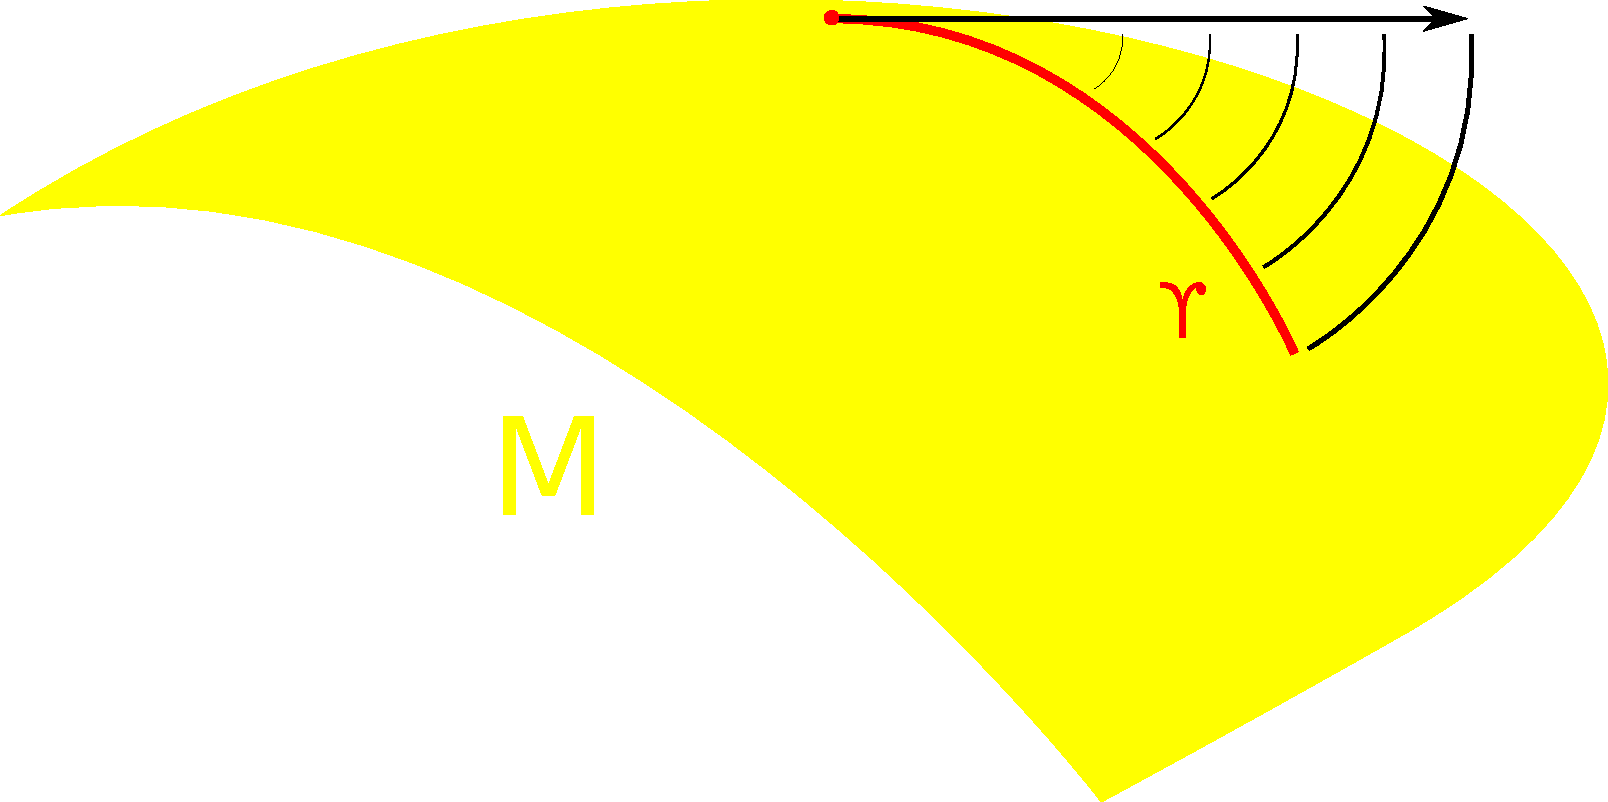
\includegraphics[scale=0.3]{fibrado_tang.pdf}
	\caption{Equivalência homotópica entre uma geodésica $\gamma\in M^{I}$ e seu vetor tangente em $\gamma(0)$.}
\end{figure}

\par Deste modo, a proposição \ref{fht_tang} nos permite afirmar que a noção de fibrado tangente pode ser extendida do conceito de variedades suaves para variedades topológicas.

\begin{prop}\label{iso_homeo}
	Se $h:M\to N$ é um homeomorfismo entre variedades topológicas, então $(\tau M,\tau_{0}M)\sim_{f}h^{*}(\tau N,\tau_{0}N)$.
\end{prop}
\begin{proof}
	
	\
	
	\par Uma vez que $h$ é um homeomorfismo, fica bem definido, o também homeomorfismo, $H:(TM,T_{0}M)\to (TN,T_{0}N)$ dado por $H(\omega)=h\circ\omega$, em que sua aplicação inversa $H^{-1}:(TN,T_{0}N)\to (TM,T_{0}M)$ é dada por $H^{-1}(\omega)=h^{-1}\circ\omega$.
	
	\par Por fim, se denotarmos por $p:TM\to M$ e $q:TN\to N$ as projeções de $(\tau M,\tau_{0}M)$ e $(\tau N,\tau_{0}N)$,  respectivamente, então a aplicação $h^{-1}\circ q\circ H:TM\to M$ será tal que $h^{-1}\circ q\circ H(\omega)=p(\omega)$.
	
	\par Assim, o lema \ref{iso_homot_2} garantirá que $(\tau M,\tau_{0}M)\sim_{f}h^{*}(\tau N,\tau_{0}N)$.
	
\end{proof}

\par Vejamos que a noção de fibrado generalizado tangente é natural com respeito ao cartesiano de variedades topológicas, no seguinte sentido:

\begin{prop}\label{fht_tang_cart}
	Sejam $M$ e $S$ duas variedades topológicas quaisquer. Então:
	
	$$ (\tau (M\times S),\tau_{0}(M\times S))\sim_{f} (\tau M,\tau_{0}M)\times (\tau S,\tau_{0}S) $$
\end{prop}
\begin{proof}
	
	\
	
	\par Inicialmente, considere $(\tau M,\tau_{0}M)=(TM,T_{0}M,p,M)$, $(\tau S,\tau_{0}S)=(TS,T_{0}S,q,S)$, $(\tau (M\times S),\tau_{0}(M\times S))=(T(M\times S),T_{0}(M\times S),r,M\times S)$ e denotemos o produto $(\tau M,\tau_{0}M)\times (\tau S,\tau_{0}S)=(E,E_{0},p\times q,M\times S)$, em que: \newline
	
	$ E=(TM)\times(TS) $
	
	$ E_{0}=[(TM)\times (T_{0}S)]\bigcup [(T_{0}M)\times (TS)] $ \newline
	
	\par Deste modo, fica bem definida a aplicação $\phi:(T(M\times S),T_{0}(M\times S))\to (E,E_{0})$ dada por $\phi(\omega)=(p_{1}\circ\omega,p_{2}\circ\omega)$, uma vez que se $\omega\in T_{0}(M\times S)$, então $\omega(t)\neq \omega(0)$ para todo $0<t\leq 1$, ou seja, $p_{i}\circ\omega(t)\neq p_{i}\circ\omega(0)$ para todo $0<t\leq 1$ e $i=1$ ou $2$, e assim, $p_{i}\circ\omega\in E_{0}$ para $i=1$ ou $2$.
	
	\par Por outro lado, observe que $\phi$ é um homeomorfismo em que sua aplicação inversa $\phi^{-1}:(E,E_{0})\to (T(M\times S),T_{0}(M\times S))$ é, naturalmente, dada por $\phi^{-1}(\omega_{1},\omega_{2})=(\omega_{1},\omega_{2})$. Ainda, é claro que $(p\times q)\circ\phi=r$.
	
	\par Assim, segue do lema \ref{iso_homot} que $(\tau (M\times S),\tau_{0}(M\times S))\sim_{f} (\tau M,\tau_{0}M)\times (\tau S,\tau_{0}S)$.
	
\end{proof}



% ------------------------------------------------------------------------------------------
% ------------------------------------------------------------------------------------------
% ------------------------------------------------------------------------------------------



\subsection{Fibrado Normal de um Mergulho Local-Flat}\label{secao_fht_normal}

\

\par Nesta subseção, mostraremos que o conceito de fibrado generalizado\index{fibrado!generalizado} também permite generalizar a noção de fibrado vetorial normal\index{fibrado!vetorial!normal} de variedades suaves\index{variedade!suave} para variedades topológicas\index{variedade!topológica}.

\par Mas antes, recordemos\footnote{Para mais detalhes, ver (\cite{lee_s}, Proposição 5.16, p. 106).} que se $M^{m}$ e $S^{m+k}$ são variedades suaves e se $i:M\hookrightarrow S$ é um mergulho suave\index{mergulho!suave}, então $i(M)$ será uma subvariedade suave de $S$ de modo que, para todo $b\in M$, existe uma vizinhança aberta $U\subset S$ de $i(b)$ tal que $(U,U\cap i(M))\approx (\R^{m+k},\R^{m})$.

\par Esta característica nos induz a seguinte:

\begin{defi}
	Um mergulho topológico\index{mergulho!topológico} $i:M^{m}\hookrightarrow S^{m+k}$, entre variedades topológicas, é dito locally-flat, ou apenas local-flat\index{mergulho!local-flat}, se para todo $b\in M$, existir uma vizinhança aberta $U\subset S$ de $i(b)$ tal que $(U,U\cap i(M))\approx (\R^{m+k},\R^{m})$.
\end{defi}

\par Nas notações da definição acima, como $M\approx i(M)$, então podemos reescrever $M^{m}\subset S^{m+k}$ como um mergulho local-flat de modo que $(U,U\cap M)\approx (\R^{m+k},\R^{m})$. A notação que será usada para descrever um mergulho local-flat dependerá do problema em questão.

%	\par Agora, vejamos alguns exemplos de mergulho que são, ou não, local-flat:
%	
%	\begin{ex}
%		
%		\
%		
%		\begin{enumerate}
%			\item Todo mergulho suave, entre variedades suaves, é local-flat.
%			\item Se $M^{m}\subset S^{m+k}$ é um mergulho topológico, entre variedades topológicas, com $M$ tendo bordo $\partial M\neq \emptyset$, então este mergulho não será local-flat.
%			\item Se $M^{m}$ é uma variedade topológica com bordo $\partial M\neq \emptyset$, então a inclusão natural $\partial M\subset M$ não é um mergulho local-flat.
%			\item Considere a inclusão não natural $i:\mathbb{S}^{1}\hookrightarrow D^{2}$, do bordo $\mathbb{S}^{1}=\partial D^{2}$ em $D^{2}$, dada por $i(x,y)=\frac{1}{2}(x,y)$. Então, $i$ é um mergulho local-flat.
%		\end{enumerate}
%	\end{ex}
%	\begin{proof}
%		
%		\
%		
%		\begin{enumerate}
%			\item Segue diretamente da definição de mergulho local-flat.
%			\item Caso $M^{m}\subset S^{m+k}$ fosse local-flat, então teríamos que para todo $b\in M$ existiria uma vizinhança $U\subset S$ de $b$ tal que $(U,U\cap M)\approx (\R^{m+k},\R^{m})$, o que não ocorre quando $b\in\partial M$, pois $U\cap M$ não pode ser homeomorfo a $\R^{m}$.
%			\item O mergulho natural $(\partial M)^{m-1}\subset M^{m}$ não pode ser local-flat, pois nenhum $b\in\partial M$ pode admitir uma vizinhança $U\subset M$ de modo que $U\approx\R^{m}$.
%			\item Inicialmente, é claro que $i:\mathbb{S}^{1}\hookrightarrow D^{2}$ é um mergulho topológico. Ainda, dado $b\in\mathbb{S}^{1}$, $U_{i(b)}=\{ p\in D^{2} \ : \ \| p-i(b)\| \leq \frac{1}{4} \}$ será uma vizinhança de $i(b)$ em $D^{2}$. Deste modo, $U_{i(b)}\cap i(\mathbb{S}^{1})$ será um arco aberto de $i(\mathbb{S}^{1})\approx \mathbb{S}^{1}$.
%			Assim, $(U_{i(b)},U_{i(b)}\cap i(\mathbb{S}^{1}))\approx (\R^{2},\R)$, ou seja, $i$ é um mergulho local-flat.
%		\end{enumerate}
%		
%	\end{proof}

\par Para o próximo resultado, considere:

\begin{itemize}
	\item $M^{m}\subset S^{m+k}$ um mergulho local-flat
	\item $N_{0}=\{ \omega\in S^{I} \ : \ \omega(t)\in M \Leftrightarrow t=0 \}$
	\item $N=N_{0}\bigcup \{ \omega\in S^{I} \ : \ \omega(t)=\omega(0)\in M, \ \forall t\in I \}$
	\item $q:N\to M$ dada por $q(\omega)=\omega(0)$
\end{itemize}

\par Assim:

\begin{prop}
	Seja $M^{m}\subset S^{m+k}$ é um mergulho local-flat\index{mergulho!local-flat}. Então, o par $(\mathcal{N},\mathcal{N}_{0})=(N,N_{0},q,M)$ será um $\R^{k}-$fibrado generalizado localmente trivial\index{localmente trivial}.
\end{prop}

\par A prova da proposição acima pode ser encontrada em (\cite{fadell_1}, Proposição 4.1, p. 496).

\begin{defi}
	Chamamos $(\mathcal{N},\mathcal{N}_{0})$ de $\R^{k}-$fibrado generalizado normal\index{fibrado!generalizado!normal} do mergulho local-flat $M^{m}\subset S^{m+k}$.
\end{defi}

\par Por outro lado, considere $M^{m}\subset\R^{m+k}$ um mergulho suave\index{mergulho!suave}, de uma variedade suave\index{variedade!suave} num espaço Euclidiano, e $\eta$ o $\R^{k}-$fibrado vetorial\index{fibrado!vetorial!normal} normal desse mergulho, como na definição \ref{defi_fvn}. Com isso, temos a seguinte relação entre o fibrado vetorial normal e o fibrado generalizado normal do mergulho local-flat $M\subset \R^{m+k}$:

\begin{prop}
	$(\eta,\eta_{0})\sim_{f} (\mathcal{N}.\mathcal{N}_{0})$
\end{prop}

\par A prova da proposição acima pode ser encontrada em (\cite{fadell_1}, Corolário 4.9, p. 498).

\par Em (\cite{fadell_1}, Teorema 4.11, p. 498), Fadell mostra que o teorema \ref{dualidade_whitney_vet} é válido no contexto de mergulhos local-flat, como no seguinte:

\begin{teo}\label{iso_merg_lf_1}
	Se $M^{m}\subset S^{m+k}$ é um mergulho local-flat com $\R^{k}-$fibrado generalizado normal $(\mathcal{N},\mathcal{N}_{0})$, então:
	$$ (\tau M,\tau_{0}M)\oplus (\mathcal{N},\mathcal{N}_{0})\sim_{f} (\tau S,\tau_{0}S)_{|M} $$
\end{teo}

\par Ainda, podemos obter a seguinte:

\begin{prop}\label{iso_merg_lf_2}
	Se $i:M^{m}\hookrightarrow S^{m+k}$ é um mergulho local-flat\index{mergulho!local-flat}, então:
	$$ (\tau S,\tau_{0}S)_{|M}\sim_{f} i^{*}(\tau S,\tau_{0}S) $$
\end{prop}
\begin{proof}
	
	\
	
	\par Primeiramente, fixemos as seguintes notações:
	
	\begin{enumerate}
		\item $(\tau S,\tau_{0}S)=(T,T_{0},p,S)$, em que:
		\begin{itemize}
			\item $T_{0}=\{ \omega\in S^{I} \ : \ \omega(t)=\omega(0) \Leftrightarrow t=0 \}$
			\item $T=T_{0}\bigcup \{ \omega\in S^{I} \ : \ \omega(t)=\omega(0), \ \forall t\in I \}$
			\item $p:T\to S$ dada por $p(\omega)=\omega(0)$
		\end{itemize}
		\item $(\tau S,\tau_{0}S)_{|M}=(p^{-1}(M),p^{-1}(M)\cap T_{0},q,M)$, em que:
		\begin{itemize}
			\item $p^{-1}(M)=\{ \omega\in T \ : \ \omega(0)\in M \}$
			\item $p^{-1}(M)\cap T_{0}=\{ \omega\in T_{0} \ : \ \omega(0)\in M \}$
			\item $q=p_{|p^{-1}(M)}:p^{-1}(M)\to M$ dada por $q(\omega)=\omega(0)$
		\end{itemize}
		\item $i^{*}(\tau S,\tau_{0}S)=(i^{*}T,i^{*}T_{0},p_{1},M)$, em que:
		\begin{itemize}
			\item $i^{*}T=\{ (b,\omega)\in M\times T \ : \ i(b)=\omega(0) \}$
			\item $i^{*}T_{0}=\{ (b,\omega)\in i^{*}T \ : \ \omega\in T_{0} \}$
			\item  $p_{1}:i^{*}T\to M$ dada por $p_{1}(b,\omega)=b$
		\end{itemize}
	\end{enumerate}
	
	\par Assim, fica bem definida a aplicação fibrada $\phi:(p^{-1}(M),p^{-1}(M)\cap T_{0})\to (i^{*}T,i^{*}T_{0})$ dada por $\phi(\omega)=(\omega(0),\omega)$.
	Por outro lado, note que também fica bem definida a aplicação $\psi:(i^{*}T,i^{*}T_{0})\to (p^{-1}(M),p^{-1}(M)\cap T_{0})$ dada por $\psi(b,\omega)=\omega$.
	
	\par Ainda, é claro que $\phi$ é um homeomorfismo com inversa $\psi$. Logo, o lema \ref{iso_homot} garante que $(\tau S,\tau_{0}S)_{|M}\sim_{f} i^{*}(\tau S,\tau_{0}S)$.
	
\end{proof}

\par Com isso, concluímos nesse capítulo os estudos sobre fibrados generalizados\index{fibrado!generalizado}, conceito desenvolvido por Fadell em \cite{fadell_1} com o intuito de generalizar as noções de fibrados vetoriais tangente\index{fibrado!vetorial!tangente} e normal\index{fibrado!vetorial!normal} do contexto de variedades suaves\index{variedade!suave} para variedades topológicas\index{variedade!topológica}, sendo que apresentamos aqui apenas a prova intuitiva, baseada nas ideias de Nash em \cite{nash}, sobre como ocorre a generalização do fibrado vetorial tangente.

\par Com o intuito de fazermos não só uma releitura numa linguagem mais moderna da primeira metade dos resultados apresentados pro Fadell em \cite{fadell_1}, mas de fazermos também uma complementação de \cite{fadell_1}, tomamos o cuidado de mostrar detalhadamente como os fibrados generalizados de fato generalizam os fibrados vetoriais\index{fibrado!vetorial}, bem como a noção de isomorfismo de fibrados vetoriais se mantém quando à extendemos para a categoria de fibrados generalizados.

\par Vale destacar que também desenvolvemos nesse capítulo o conceito de fibrado generalizado pullback\index{fibrado!generalizado!pullback}, bem como algumas consequências de tal fibrado, conceito esse que em nenhum momento foi citado por Fadell em \cite{fadell_1}.

\par De todo modo, os resultados sobre fibrados generalizados desenvolvidos cuidadosamente nesse capítulo sugerem olharmos para esse conceito como uma teoria em si e não apenas como uma ferramenta para construirmos as classes características conforme apresentaremos no capítulo a seguir.





% ---------------------------------------------------------------------------------------------------
% ---------------------------------------------------------------------------------------------------
% -----------------------------------------------   CLASSES CARACTERÍSTICAS DE VARIEDADES TOPOLÓGICAS
% ---------------------------------------------------------------------------------------------------
% ---------------------------------------------------------------------------------------------------





\chapter{Classes Características de Variedades Topológicas}\label{cap_clas_carac}
\thispagestyle{empty}

\

\par Neste capítulo, iremos construir as classes de Thom\index{classe!de Thom}, de Stiefel-Whitney\index{classe!de Stiefel-Whitney} e de Euler\index{classe!de Euler} de fibrados generalizados\index{fibrado!generalizado} e apresentar algumas consequências de tais objetos. Em particular, veremos o comportamento dessas classes para os fibrados generalizados tangentes\index{fibrado!generalizado!tangente} de variedades topológicas\index{variedade!topológica}.

\par Para tanto, introduziremos na seção \ref{secao_thom} o conceito de orientabilidade de fibrados generalizados, que foi proposto originalmente por Fadell em \cite{fadell_1}, a fim de garantirmos a existência da classe e do isomorfismo de Thom de tais fibrados. Também veremos como a classe de Thom se comporta em fibrados generalizados específicos.

\par Já na seção \ref{secao_SW}, definiremos as classes de Stiefel-Whitney de fibrados generalizados de forma idêntica a definição das classes de Stiefel-Whitney de fibrados vetoriais\index{fibrado!vetorial} apresentada em \cite{milnor_1}. Ainda, veremos como a noção do fibrado generalizado pullback apresentada no capítulo anterior será relevante para concluirmos algumas consequências das classes de Stiefel-Whitney, uma vez que Fadell não abordou esse conceito em \cite{fadell_1}.

\par Encerrando o capítulo, definiremos na seção \ref{secao_euler} a classe de Euler de fibrados generalizados, sendo tal classe muito pouco abordada por Fadell em \cite{fadell_1}. Nessa seção, apresentaremos vários resultados conhecidos sobre classes de Euler de fibrados vetoriais e de variedades suaves, porém em suas versões para de fibrados generalizados e de variedades topológicas.

\par Como explicado na observação \ref{obs_varied_bordo}, vamos ressaltar que toda variedade topológica citada nesse capítulo será uma variedade sem bordo.


% ------------------------------------------------------------------------------------------
% ------------------------------------------------------------------------------------------
% ------------------------------------------------------------------------------------------



\section{Orientabilidade e Classe de Thom}\label{secao_thom}

\

\par Antes de construirmos as classes de Stiefel-Whitney\index{classe!de Stiefel-Whitney} e de Euler\index{classe!de Euler} de fibrados generalizados\index{fibrado!generalizado}, precisamos introduzir o conceito de orientabilidade desses fibrados. Tal conceito será fundamental para garantir a existência da classe\index{classe!de Thom} e do isomorfismo de Thom\index{isomorfismo!de Thom}, como será visto mais adiante.

\par O conceito de orientabilidade de fibrados generalizados foi proposto por Fadell em \cite{fadell_1}. Entretanto, Fadell não se aprofundou muito nessa questão, uma vez que o tema principal desenvolvido em \cite{fadell_1} foi sobre classes de Stiefel-Whitney e, nesse sentido, não há a necessidade de se preocupar com a orientabilidade.

\par Nesta seção vamos abordar com um pouco mais de detalhes a noção de orientabilidade de fibrados generalizados e apresentar alguns resultados técnicos sobre a classe de Thom, mais especificamente, qual o comportamento da classe de Thom nos fibrados generalizados pullback\index{fibrado!generalizado!pullback} e produto\index{fibrado!generalizado!produto}, o que ocorre quando invertemos a orientabilidade de um fibrado generalizado e qual a relação entre a dimensão de uma variedade topológica e a classe de Thom do seu fibrado generalizado tangente\index{fibrado!generalizado!tangente}.

\par Com exceção dos lemas \ref{lema_thom_2}, \ref{lema_thom_3}, \ref{lema_thom_4} e \ref{lema_thom_5}, os resultados apresentados nessa seção foram retirados de \cite{fadell_1}.

\par Assim, consideremos primeiramente $(\mathcal{F},\mathcal{F}_{0})=(E,E_{0},p,B)$ um $\R^{n}-$fibrado generalizado\index{fibrado!generalizado} e o seguinte conjunto:
$$ \Omega_{p}=\{ (e,\omega)\in E\times B^{I} \ : \ p(e)=\omega(0) \} $$

\par Em particular, como  $(\mathcal{F},\mathcal{F}_{0})$ é uma fibração de pares\index{fibração!de pares}, então ao definirmos as aplicações $h:\Omega_{p}\to E$ e $H:\Omega_{p}\times I\to B$, respectivamente, por $h(e,\omega)=e$ e $H((e,\omega),t)=\omega(t)$, então existirá uma aplicação $\wt{H}:\Omega_{p}\times I\to E$ tal que o seguinte diagrama comuta:

$$ \xymatrix @C=0.5cm {
	\Omega_{p}\times \{0\}\ar[rrrrr]^-{h} \ar@{^(->}[ddd] &&&&& E \ar[ddd]^-{p} \\
	&&&&& \\		 
	&&&&& \\				 
	\Omega_{p}\times I \ar[rrrrr]^-{H} \ar[rrrrruuu]^-{\wt{H}} &&&&& B
} $$

\par Ainda, se $(e,\omega)\in \Omega_{p}$ é tal que $h(e,\omega)\in E_{0}$, então sabemos que $\wt{H}((e,\omega),\_)\in E_{0}$. Deste modo, podemos definir a aplicação $\lambda:\Omega_{p}\to E^{I}$ por $\left[ \lambda(e,\omega) \right](t)=\wt{H}((e,\omega),t)$.

\par Assim, fixada a fibra $(F,F_{0})$ de $(\mathcal{F},\mathcal{F}_{0})$ sobre $b_{0}\in B$, fica bem definida a seguinte aplicação:
$$ \Omega(B,b_{0})\times (F,F_{0}) \to (F,F_{0}) $$
$$ (\omega,e)\longmapsto \omega\cdot e=[\lambda(e,\omega)](1) $$

\par Note que, fixando $\omega\in \Omega(B,b_{0})$, é evidente que a aplicação $(F,F_{0})\to (F,F_{0})$, que associa $e\mapsto \omega\cdot e$, induz uma ação de $\Omega(B,b_{0})$ em $H_{n}(F,F_{0};R)$ para qualquer anel $R$ comutativo e com unidade.

\par Com isso, temos a seguinte:

\begin{defi}{\bf (Orientabilidade)}\label{defi_orient}
	Um $\R^{n}-$fibrado generalizado $(\mathcal{F},\mathcal{F}_{0})$ sobre $B$ é dito $R-$orientável\index{fibrado!generalizado!orientável} se para todo $b_{0}\in B$, a ação acima definida de $\Omega(B,b_{0})$ em $H_{n}(F,F_{0};R)$ é trivial, em que $(F,F_{0})$ denota a fibra de $(\mathcal{F},\mathcal{F}_{0})$ sobre $b_{0}\in B$.
\end{defi}

\par Naturalmente, a orientação de uma variedade topológica\index{variedade!topológica} está diretamente relacionada com a orientação do seu respectivo fibrado generalizado tangente\index{fibrado!generalizado!tangente}, como enunciaremos no próximo resultado e cuja prova pode ser encontrada em (\cite{fadell_1}, Proposição 3.16, p. 495).

\begin{prop}\label{propriedade_orient_var}
	Uma variedade topológica $M$ é $R-$orientável se, e somente se, seu fibrado generalizado tangente $(\tau M,\tau_{0}M)$ é $R-$orientável.
\end{prop}

\begin{obs}
	Todo fibrado generalizado é $\Z_{2}-$orientável, como garantido em (\cite{allaud}, Corolário 2.8, p. 243).
\end{obs}

\par Com o intuito de definirmos as classes de Stiefel-Whitney\index{classe!de Stiefel-Whitney} de um fibrado generalizado qualquer e a classe de Euler\index{classe!de Euler} de um fibrado generalizado $\Z-$orientável, precisamos garantir a existência da classe e do isomorfismo de Thom, do mesmo modo que é feita a construção destas classes para fibrados vetoriais\index{fibrado!vetorial}, como em (\cite{milnor_1}, Capítulos 8,9 e 10).

\begin{teo}\label{teo_iso_thom_fht}
	Seja $(\mathcal{F},\mathcal{F}_{0})=(E,E_{0},p,B)$ um $\R^{n}-$fibrado generalizado $R-$orientável. Então, existe uma única classe $\tau\in H^{n}(E,E_{0};R)$ tal que $\phi:H^{k}(B;R)\to H^{n+k}(E,E_{0};R)$, dado por $\phi(x)=p^{*}(x)\ccup \tau$, é um isomorfismo para todo inteiro $k\geq 0$. Ainda, sendo $i:(F,F_{0})\hookrightarrow (E,E_{0})$ a inclusão de uma fibra $(F,F_{0})$ de $(\mathcal{F},\mathcal{F}_{0})$ em seu espaço total e $(u)=H^{n}(F,F_{0};R)\cong R$, então a classe $\tau$ é unicamente determinada por $i^{*}(\tau)=u$.
\end{teo}

\par A prova do teorema acima pode ser encontrada em (\cite{fadell_1}, Teorema 5.2, p. 502).

\begin{obs}\label{obs_proj_iso}
	No decorrer da demonstração do teorema \ref{teo_iso_thom_fht}, é mostrado que as induzidas $i^{*}:H^{n}(E,E_{0};R)\to H^{n}(F,F_{0};R)$ e $p^{*}:H^{k}(B;R)\to H^{k}(E;R)$ são isomorfismos para todo $k\geq 0$.
\end{obs}

\begin{defi}{\bf (Classe e Isomorfismo de Thom)}\label{defi_thom}
	Dado um $\R^{n}-$fibrado generalizado $(\mathcal{F},\mathcal{F}_{0})=(E,E_{0},p,B)$ $R-$orientável, chamamos o gerador $(\tau)=H^{n}(E,E_{0};R)\cong R$ e o isomorfismo $\phi:H^{k}(B;R)\to H^{n+k}(E,E_{0};R)$, dados no teorema \ref{teo_iso_thom_fht}, por classe\index{classe!de Thom} e isomorfismo\index{isomorfismo!de Thom} de Thom de $(\mathcal{F},\mathcal{F}_{0})$, respectivamente.
\end{defi}

\par Agora, vejamos algumas consequências envolvendo orientabilidade e as classes de Thom de fibrados generalizados. Como vamos trabalhar com classes de Stiefel-Whitney\index{classe!de Stiefel-Whitney} e de Euler\index{classe!de Euler} no decorrer deste capítulo, então os lemas finais dessa seção serão feitos para $R=\Z_{2}$ e $R=\Z$.

%\begin{lem}\label{lema_thom_1}
%Sejam $(\mathcal{F},\mathcal{F}_{0})$ e $(\mathcal{F'},\mathcal{F'}_{0})$ dois $\R^{n}-$fibrados generalizados sobre a mesma base tais que $(\mathcal{F},\mathcal{F}_{0})\sim_{f}(\mathcal{F'},\mathcal{F'}_{0})$. Então:
%	\begin{enumerate}
%		\item $(\mathcal{F},\mathcal{F}_{0})$ é $R-$orientável se, e somente se, $(\mathcal{F'},\mathcal{F'}_{0})$ é $R-$orientável;
%		\item sendo $(\mathcal{F},\mathcal{F}_{0})$ $R-$orientável\index{fibrado!generalizado!orientável} e denotando por $\tau$ e $\tau'$ as classes de Thom\index{classe!de Thom} de $(\mathcal{F},\mathcal{F}_{0})$ e $(\mathcal{F'},\mathcal{F'}_{0})$, respectivamente, então a aplicação fibrada $f:(\mathcal{F},\mathcal{F}_{0})\to (\mathcal{F'},\mathcal{F'}_{0})$ garantida pela definição \ref{defi_iso_homot} é tal que $f^{*}(\tau')=\tau$.
%	\end{enumerate}
%\end{lem}
%\begin{proof}
%
%\
%
%\par A
%
%\end{proof}

\begin{lem}\label{lema_thom_2}
	Sejam $(\mathcal{F},\mathcal{F}_{0})$ um $\R^{n}-$fibrado generalizado $R-$orientável\index{fibrado!generalizado!orientável} sobre uma base $B$, $f:B'\to B$ uma aplicação qualquer e $\tau$ a classe de Thom\index{classe!de Thom} de $(\mathcal{F},\mathcal{F}_{0})$. Assim:
	\begin{enumerate}
		\item $f^{*}(\mathcal{F},\mathcal{F}_{0})$ será um $\R^{n}-$fibrado generalizado $R-$orientável;
		\item sendo $\tau^{*}$ a classe de Thom de $f^{*}(\mathcal{F},\mathcal{F}_{0})$, então $\tau^{*}=1\times \tau$.
	\end{enumerate}
\end{lem}
\begin{proof}
	
	\
	
	\par Primeiramente, denotando $(\mathcal{F},\mathcal{F}_{0})=(E,E_{0},p,B)$, já sabemos pelo lema \ref{fht_pullback} que $f^{*}(\mathcal{F},\mathcal{F}_{0})=(f^{*}E,f^{*}E_{0},p_{1},B')$ será um $\R^{n}-$fibrado generalizado, em que: \newline
	
	$f^{*}E=\{ (b',e)\in B'\times E \ : \ f(b')=p(e) \}$
	
	$f^{*}E_{0}=\{ (b',e)\in f^{*}E \ : \ e\in E_{0} \}$ \newline
	
	\par Agora, fixados $b'_{0}\in B'$ e $f(b'_{0})\in B$, consideremos $(F^{*},F^{*}_{0})$ e $(F,F_{0})$ as fibras de $f^{*}(\mathcal{F},\mathcal{F}_{0})$ e $(\mathcal{F},\mathcal{F}_{0})$ sobre $b'_{0}\in B'$ e $f(b'_{0})\in B$, respectivamente. Devido ao lema \ref{pf_pullback}, também sabemos que $(F^{*},F^{*}_{0})=\{ b'_{0} \}\times (F,F_{0})$.
	
	\par Assim, a ação dada na definição \ref{defi_orient} de $\Omega(B',b'_{0})$ em $H_{n}(F^{*},F^{*}_{0};R)$ se resume a ação de $\Omega(B,f(b'_{0}))$ em $H_{n}(F,F_{0};R)$.
	
	\par Como $(\mathcal{F},\mathcal{F}_{0})$ é um fibrado generalizado $R-$orientável, então a ação de $\Omega(B,f(b'_{0}))$ em $H_{n}(F,F_{0};R)$ é trivial. Com isso, a ação de $\Omega(B',b'_{0})$ em $H_{n}(F^{*},F^{*}_{0};R)$ será trivial e, consequentemente, $f^{*}(\mathcal{F},\mathcal{F}_{0})$ será um fibrado generalizado $R-$orientável.
	
	\par Por fim, denotando as classes de Thom\index{classe!de Thom} de $(\mathcal{F},\mathcal{F}_{0})$ e $f^{*}(\mathcal{F},\mathcal{F}_{0})$ respectivamente pelos geradores $(\tau)=H^{n}(E,E_{0};R)$ e $(\tau^{*})=H^{n}(f^{*}E,f^{*}E_{0};R)$, provemos que $\tau^{*}=1\times\tau$.
	
	\par Para tanto, consideremos $i:(F,F_{0})\hookrightarrow (E,E_{0})$ e $j:(F^{*},F^{*}_{0})\hookrightarrow (f^{*}E,f^{*}E_{0})$ as inclusões canônicas. Como $(F^{*},F^{*}_{0})=\{ b'_{0} \}\times (F,F_{0})$, então $j=1\times i$.
	
	\par Agora, fixando os geradores $(u)=H^{n}(F,F_{0};R)$ e $(1\times u)=H^{n}(F^{*},F^{*}_{0};R)$\footnote{A fórmula de Künneth\index{fórmula!de Künneth} nos permite afirmar que $1\times u$ será um gerador de $H^{n}(F^{*},F^{*}_{0};R)$.}, lembremos que as classe de Thom $\tau$ e $\tau^{*}$ são unicamente determinadas de modo que $i^{*}(\tau)=u$ e $j^{*}(\tau^{*})=1\times u$.
	
	\par Entretanto, veja que:\newline
	
	$\begin{array}{rl}
		j^{*}(1\times \tau) \ = & (1\times i)^{*}(1\times \tau) \\
		= & 1\times i^{*}(\tau) \\
		= & 1\times u
	\end{array}$ \newline
	
	\par Logo, concluímos por unicidade que $\tau^{*}=1\times \tau$.
	
\end{proof}

\begin{lem}\label{lema_thom_3}
	Sejam $(\mathcal{F},\mathcal{F}_{0})$ um $\R^{n}-$fibrado generalizado\index{fibrado!generalizado!orientável}, $(\mathcal{F'},\mathcal{F'}_{0})$ um $\R^{m}-$fibrado generalizado, ambos $R-$orientáveis. Denotando por $\tau$ e $\tau'$ as classes de Thom\index{classe!de Thom} de $(\mathcal{F},\mathcal{F}_{0})$ e $(\mathcal{F'},\mathcal{F'}_{0})$, respectivamente, então:
	\begin{enumerate}
		\item $(\mathcal{F},\mathcal{F}_{0})\times (\mathcal{F'},\mathcal{F'}_{0})$ será um $\R^{n+m}-$fibrado generalizado $R-$orientável;
		\item sendo $\tau''$ a classe de Thom de $(\mathcal{F},\mathcal{F}_{0})\times (\mathcal{F'},\mathcal{F'}_{0})$, então $\tau''=\tau\times\tau'$.
	\end{enumerate}
\end{lem}
\begin{proof}
	
	\
	
	\par Inicialmente, recordando o lema \ref{fht_produto}, já sabemos que $(\mathcal{F},\mathcal{F}_{0})\times (\mathcal{F'},\mathcal{F'}_{0})$ será um $\R^{n+m}-$fibrado generalizado. Ainda, denotaremos $(\mathcal{F},\mathcal{F}_{0})=(E,E_{0},p,B)$, $(\mathcal{F'},\mathcal{F'}_{0})=(E',E'_{0},q,B')$ e $(\mathcal{F},\mathcal{F}_{0})\times (\mathcal{F'},\mathcal{F'}_{0})=(E'',E''_{0},r,B'')$, em que: \newline
	
	$E''=E\times E'$
	
	$E''_{0}=\left( E\times E'_{0} \right)\bigcup \left( E_{0}\times E' \right)$
	
	$r=p\times q$
	
	$B''=B\times B'$ \newline
	
	\par Fixando $b_{0}\in B$, $b'_{0}\in B'$ e $(b_{0},b'_{0})\in B''$, consideremos $(F,F_{0})$, $(F',F'_{0})$ e $(F'',F''_{0})$ as fibras de $(\mathcal{F},\mathcal{F}_{0})$, $(\mathcal{F'},\mathcal{F'}_{0})$ e $(\mathcal{F},\mathcal{F}_{0})\times (\mathcal{F'},\mathcal{F'}_{0})$ sobre $b_{0}\in B$, $b'_{0}\in B'$ e $(b_{0},b'_{0})\in B''$, respectivamente.
	
	\par Como $(F'',F''_{0})=(F,F_{0})\times (F',F'_{0})$, então a fórmula de Künneth\index{fórmula!de Künneth} nos garantirá que:
	$$ H_{n+m}(F'',F''_{0};R)\cong H_{n}(F,F_{0};R)\tensor H_{m}(F',F'_{0};R) $$
	
	\par Ainda, também temos o seguinte homeomorfismo:
	$$ \Omega(B'',(b_{0},b'_{0}))\approx \Omega(B,b_{0})\times\Omega(B',b'_{0}) $$
	
	\par Deste modo, a ação dada na definição \ref{defi_orient} de $\Omega(B'',(b_{0},b'_{0}))$ em $H_{n+m}(F'',F''_{0};R)$ se resume as ações de $\Omega(B,b_{0})$ e $\Omega(B',b'_{0})$ em $H_{n}(F,F_{0};R)$ e $H_{m}(F',F'_{0};R)$, respectivamente.
	
	\par Como $(\mathcal{F},\mathcal{F}_{0})$ e $(\mathcal{F'},\mathcal{F'}_{0})$ são fibrados generalizados $R-$orientáveis, então as ações de $\Omega(B,b_{0})$ e $\Omega(B',b'_{0})$ em $H_{n}(F,F_{0};R)$ e $H_{m}(F',F'_{0};R)$, respectivamente, são triviais. Assim, a ação de $\Omega(B'',(b_{0},b'_{0}))$ em $H_{n+m}(F'',F''_{0};R)$ será trivial e, consequentemente, $(\mathcal{F},\mathcal{F}_{0})\times (\mathcal{F'},\mathcal{F'}_{0})$ será um fibrado generalizado $R-$orientável.
	
	\par Por fim, denotando os geradores $(\tau)=H^{n}(E,E_{0};R)$, $(\tau')=H^{m}(E',E'_{0};R)$ e $(\tau'')=H^{n+m}(E'',E''_{0};R)$ como sendo as classes de Thom de $(\mathcal{F},\mathcal{F}_{0})$, $(\mathcal{F'},\mathcal{F'}_{0})$ e $(\mathcal{F},\mathcal{F}_{0})\times (\mathcal{F'},\mathcal{F'}_{0})$, respectivamente, provemos que $\tau''=\tau\times\tau'$.
	
	\par Para tanto, vamos considerar $i:(F,F_{0})\hookrightarrow (E,E_{0})$, $i':(F',F'_{0})\hookrightarrow (E',E'_{0})$ e $i'':(F'',F''_{0})\hookrightarrow (E'',E''_{0})$ as inclusões canônicas. Como $(F'',F''_{0})=(F,F_{0})\times (F',F'_{0})$ e $(E'',E''_{0})=(E,E_{0})\times (E',E'_{0})$, então $i''=i\times i'$.
	
	\par Agora, fixando os geradores $(u)=H^{n}(F,F_{0};R)$, $(u')=H^{m}(F',F'_{0};R)$ e $(u\times u')=H^{n+m}(F'',F''_{0};R)$\footnote{A fórmula de Künneth\index{fórmula!de Künneth} nos permite afirmar que $u\times u'$ será um gerador de $H^{n+m}(F'',F''_{0};R)$.}, lembremos que as classes de Thom $\tau$, $\tau'$ e $\tau''$ são unicamente determinadas de modo que $i^{*}(\tau)=u$, $i'^{*}(\tau')=u'$ e $i''^{*}(\tau'')=u\times u'$, respectivamente.
	
	\par Entretanto, note que: \newline
	
	$\begin{array}{rl}
		i''^{*}(\tau\times\tau') \ = & (i\times i')^{*}(\tau\times\tau') \\
		= & i^{*}(\tau)\times i'^{*}(\tau') \\
		= & u\times u'
	\end{array}$ \newline
	
	\par Assim, concluímos por unicidade que $\tau''=\tau\times\tau'$.
	
\end{proof}

\begin{lem}\label{lema_thom_4}
	Sejam $(\mathcal{F},\mathcal{F}_{0})$ um $\R^{n}-$fibrado generalizado\index{fibrado!generalizado!orientável} $\Z-$orientável e $\tau$ sua classe de Thom\index{classe!de Thom}. Denotando por $-(\mathcal{F},\mathcal{F}_{0})$ o próprio $\R^{n}-$fibrado generalizado $(\mathcal{F},\mathcal{F}_{0})$, porém com orientação invertida, e $\tau'$ sua classe de Thom, então $\tau'=-\tau$.
\end{lem}
\begin{proof}
	
	\
	
	\par Inicialmente, denotemos por $(E,E_{0})$ o espaço total de $(\mathcal{F},\mathcal{F}_{0})$ e $(F,F_{0})$ uma fibra arbitrária de $(\mathcal{F},\mathcal{F}_{0})$.
	
	\par Assim, o resultado seguirá diretamente do teorema \ref{teo_iso_thom_fht} e da definição \ref{defi_thom}, uma vez que a classe de Thom de $(\mathcal{F},\mathcal{F}_{0})$ é o gerador $(\tau)=H^{n}(E,E_{0};\Z)\cong\Z$ que está diretamente relacionado com o gerador $(u)=H^{n}(F,F_{0};\Z)\cong\Z$ e, consequentemente, a classe de Thom de $-(\mathcal{F},\mathcal{F}_{0})$ será o gerador $(-\tau)=H^{n}(E,E_{0};\Z)\cong\Z$ que está diretamente relacionado com o gerador $(-u)=H^{n}(F,F_{0};\Z)\cong\Z$.
	
\end{proof}

\begin{lem}\label{lema_thom_5}
	Sejam $M^{m}$ é uma variedade topológica\index{variedade!topológica} fechada $\Z-$orientável de dimensão ímpar e $(\tau M,\tau_{0}M)$ seu $\R^{m}-$fibrado generalizado tangente\index{fibrado!generalizado!tangente}. Então, a classe de Thom\index{classe!de Thom} $\tau$ de $(\tau M,\tau_{0}M)$ é tal que $\tau\ccup\tau=0$.
\end{lem}
\begin{proof}
	
	\
	
	\par Primeiramente, como $M^{m}$ é uma variedade topológica $\Z-$orientável, então a proposição \ref{propriedade_orient_var} nos garante que o $\R^{m}-$fibrado generalizado tangente $(\tau M,\tau_{0}M)$ de $M$ é $\Z-$orientável.
	
	\par Por outro lado, denotando por $(TM,T_{0}M)$ o espaço total de $(\tau M,\tau_{0}M)$ e lembrando que $M$ é compacta, então o isomorfismo de Thom de $(\tau M,\tau_{0}M)$ nos garantirá que:
	$$ H^{2m}(TM,T_{0}M;\Z)\cong H^{m}(M;\Z)\cong\Z $$
	
	\par Deste modo, denotando o gerador $(\tau)=H^{m}(TM,T_{0}M;\Z)$ como sendo a classe de Thom de $(\tau M,\tau_{0}M)$, como o item 5 do lema \ref{propriedades_produtos} afirma que $\tau\ccup\tau =(-1)^{m^{2}}(\tau\ccup\tau)$ e $m$ é ímpar, então $\tau\ccup\tau=-(\tau\ccup\tau)$, ou seja, $2(\tau\ccup\tau)=0$.
	
	\par Uma vez que $2(\tau\ccup\tau)\in H^{2m}(TM,T_{0}M;\Z)\cong\Z$, então $\tau\ccup\tau=0$.
	
\end{proof}



% ------------------------------------------------------------------------------------------
% ------------------------------------------------------------------------------------------
% ------------------------------------------------------------------------------------------



\section{Classes de Stiefel-Whitney}\label{secao_SW}

\

\par A construção das classes de Stiefel-Whitney para fibrados generalizados\index{fibrado!generalizado} seguirá, devido ao teorema \ref{teo_iso_thom_fht}, de modo idêntico a construção feita em (\cite{milnor_1}, Capítulo 8) para fibrados vetoriais\index{fibrado!vetorial}. Note que, como todo fibrado generalizado é $\Z_{2}-$orientável e as classes de Stiefel-Whitney são construídas no âmbito de $\Z_{2}-$módulos de cohomologia singular, então não precisaremos impor nenhuma condição de orientabilidade nos fibrados generalizados no decorrer dessa seção.

\par Com exceção das proposições \ref{res_SW_fht_8} e \ref{res_SW_fht_9}, os resultados desta seção foram retirados de \cite{fadell_1} e \cite{fadell_4}. Ainda, vale destacar que os teoremas \ref{res_SW_fht_2} e \ref{res_SW_fht_10} e o corolário \ref{res_SW_fht_6} podem ser encontrados em (\cite{fadell_4}, Lema 2.11, p. 39), (\cite{fadell_4}, Teorema 5.2, p. 52) e (\cite{fadell_1}, Teorema 6.11, p. 504), respectivamente, sendo que Fadell apresenta provas mais técnicas sem a utilização dos fibrados generalizados pullbacks. Em contrapartida, as provas de tais resultados aqui apresentadas realçam a importância do fibrado generalizado pullback\index{fibrado!generalizado!pullback}.

\par Deste modo, sendo $(\mathcal{F},\mathcal{F}_{0})=(E,E_{0},p,B)$ um $\R^{n}-$fibrado generalizado e $\phi$ seu isomorfismo de Thom, faz sentido, para todo $k\geq 0$, a seguinte composição\footnote{$Sq^{k}$ denota a operação quadrado de Steenrod\index{quadrado de Steenrod}, cuja algumas propriedades podem sem encontradas na seção \ref{ap_steenrod}.}:
$$ \xymatrix @C=0.5cm {
	H^{n}(E,E_{0};\Z_{2}) \ar[rrr]^-{Sq^{k}} &&& H^{n+k}(E,E_{0};\Z_{2}) \ar[rrr]^-{\phi^{-1}} &&& H^{k}(B;\Z_{2})
} $$

\begin{defi}{\bf (Classes de Stiefel-Whitney)}
	Sejam $(\mathcal{F},\mathcal{F}_{0})$ um $\R^{n}-$fibrado generalizado sobre uma base $B$ e $\phi$ e $\tau$ seu isomorfismo e sua classe de Thom, respectivamente. Para cada $k\geq 0$, chamamos de $k-$ésima classe de Stiefel-Whitney\index{classe!de Stiefel-Whitney} de $(\mathcal{F},\mathcal{F}_{0})$ a seguinte classe:	
	$$ w_{k}(\mathcal{F},\mathcal{F}_{0})=\phi^{-1}\circ Sq^{k}(u)\in H^{k}(B;\Z_{2}) $$
	
	\par Ainda, chamamos o elemento $W(\mathcal{F},\mathcal{F}_{0})=\ds\sum_{k\geq 0}w_{k}(\mathcal{F},\mathcal{F}_{0})\in H^{*}(B;\Z_{2})$ de classe de Stiefel-Whitney total\index{classe!de Stiefel-Whitney total} de $(\mathcal{F},\mathcal{F}_{0})$.
\end{defi}

\par Agora, vejamos algumas consequências das classes de Stiefel-Whitney.

\begin{teo}\label{res_SW_fht_1}
	Seja $(\mathcal{F},\mathcal{F}_{0})$ um $\R^{n}-$fibrado generalizado. Então, $w_{0}(\mathcal{F},\mathcal{F}_{0})=1$ e $w_{k}(\mathcal{F},\mathcal{F}_{0})=0$ para $k>n$. Em outras palavras, $W(\mathcal{F},\mathcal{F}_{0})=1+\ds\sum_{k=1}^{n}w_{k}(\mathcal{F},\mathcal{F}_{0})$.
\end{teo}
\begin{proof}
	
	\
	
	\par Considere $(\mathcal{F},\mathcal{F}_{0})=(E,E_{0},p,B)$, $\phi$ seu isomorfismo de Thom e $\tau\in H^{n}(E,E_{0};\Z_{2})$ sua classe de Thom. Como $\phi(1)=\tau$ e $Sq^{0}=1$, então: \newline
	
	$\begin{array}{rl}
		w_{0}(\mathcal{F},\mathcal{F}_{0}) \ = & \phi^{-1}\circ Sq^{0}(\tau) \\
		= & \phi^{-1}(\tau) \\
		= & 1
	\end{array}$ \newline
	
	\par Por outro lado, para $k>n$, temos que $Sq^{k}=0$ e, assim, $w_{k}(\mathcal{F},\mathcal{F}_{0})=0$. Logo, a classe de Stiefel-Whitney total de $(\mathcal{F},\mathcal{F}_{0})$ é $W(\mathcal{F},\mathcal{F}_{0})=1+\ds\sum_{k=1}^{n}w_{k}(\mathcal{F},\mathcal{F}_{0})$.
	
\end{proof}

\par Note que, dado um $\R^{n}-$fibrado generalizado $(\mathcal{F},\mathcal{F}_{0})$ sobre $B$, como o teorema \ref{res_SW_fht_1} garante que $w_{0}(\mathcal{F},\mathcal{F}_{0})=1$, então a classe de Stiefel-Whitney total é um elemento inversível\footnote{Ver teorema \ref{teo_elemento_inversivel}.} no anel $H^{*}(B;\Z_{2})$, cujo elemento inverso será denotado por $W^{-1}(\mathcal{F},\mathcal{F}_{0})$.

\begin{teo}\label{res_SW_fht_2}
	Sejam $(\mathcal{F},\mathcal{F}_{0})$ e $(\mathcal{F'},\mathcal{F'}_{0})$ dois $\R^{n}-$fibrados generalizados sobre $B$ e $B'$, respectivamente. Se $f:B\to B'$ é uma aplicação tal que $(\mathcal{F},\mathcal{F}_{0})\sim_{f} f^{*}(\mathcal{F'},\mathcal{F'}_{0})$, então $W(\mathcal{F},\mathcal{F}_{0})=f^{*}(W(\mathcal{F'},\mathcal{F'}_{0}))$.
\end{teo}
\begin{proof}
	
	\
	
	\par Inicialmente, considere $(\mathcal{F},\mathcal{F}_{0})=(E,E_{0},p,B)$ e $(\mathcal{F'},\mathcal{F'}_{0})=(E',E'_{0},q,B')$ e recordemos que $f^{*}(\mathcal{F'},\mathcal{F'}_{0})=(f^{*}E',f^{*}E'_{0},p_{1},B)$ é o $\R^{n}-$fibrado generalizado tal que: \newline
	
	$f^{*}E'=\{ (b,e')\in B\times E' \ : \ f(b)=q(e') \}$
	
	$f^{*}E'_{0}=\{ (b,e')\in f^{*}E' \ : \ e'\in E'_{0} \}$ \newline
	
	\par Como $(\mathcal{F},\mathcal{F}_{0})\sim_{f} f^{*}(\mathcal{F'},\mathcal{F'}_{0})$, então a definição \ref{defi_iso_homot} nos garante que existe uma aplicação fibrada\index{aplicação!fibrada} $g:(E,E_{0})\to (f^{*}E',f^{*}E'_{0})$ tal que $g$ é, em particular, uma equivalência homotópica.
	
	\par Assim, considerando as classes de Thom\index{classe!de Thom} de $(\mathcal{F},\mathcal{F}_{0})$ e $f^{*}(\mathcal{F'},\mathcal{F'}_{0})$ respectivamente como sendo os geradores $(\tau)=H^{n}(E,E_{0};\Z_{2})$ e $(\tau^{*})=H^{n}(f^{*}E',f^{*}E'_{0};\Z_{2})$, então o fato de $g$ ser uma equivalência homotópica nos permite afirmar que:
	$$ g^{*}(\tau^{*})=\tau $$
	
	\par Por outro lado, considerando a classe de Thom de $(\mathcal{F'},\mathcal{F'}_{0})$ como sendo o gerador $(\tau')=H^{n}(E',E'_{0};\Z_{2})$, então o lema \ref{lema_thom_2} nos garantirá que a projeção canônica $p_{2}:(f^{*}E',f^{*}E'_{0})\to (E',E'_{0})$ é tal que:
	$$ p_{2}^{*}(\tau')=\tau^{*}=1\times \tau' $$
	
	\par Deste modo, temos que:
	$$ g^{*}\circ p_{2}^{*}(\tau')=\tau $$
	
	\par Ainda, por definição, temos o seguinte diagrama comutativo:
	$$ \xymatrix @C=0.5cm {
		E \ar[rrrrr]^-{g} \ar[rrrrrddd]^-{p} &&&&& f^{*}E' \ar[rrrrr]^-{p_{2}} \ar[ddd]^-{p_{1}} &&&&& E' \ar[ddd]^-{q} \\
		&&&&& &&&&& \\
		&&&&& &&&&& \\
		&&&&& B \ar[rrrrr]^-{f} &&&&& B'
	} $$
	
	\par Agora, denotando os isomorfismos de Thom\index{isomorfismo!de Thom} de $(\mathcal{F},\mathcal{F}_{0})$ e $(\mathcal{F'},\mathcal{F'}_{0})$ respectivamente por $\phi:H^{k}(B;\Z_{2})\to H^{k+n}(E,E_{0};\Z_{2})$ e $\phi':H^{k}(B';\Z_{2})\to H^{k+n}(E',E'_{0};\Z_{2})$, então também podemos afirmar que $\phi\circ f^{*}=g^{*}\circ p_{2}^{*}\circ\phi'$. De fato: \newline
	
	$\begin{array}{rl}
		\forall x\in H^{*}(B';\Z_{2}), \ g^{*}\circ p_{2}^{*}\circ\phi'(x) \ = & g^{*}\circ p_{2}^{*}(q^{*}(x)\ccup \tau') \\
		= & [g^{*}\circ p_{2}^{*}\circ q^{*}(x)]\ccup [g^{*}\circ p_{2}^{*}(\tau')] \\
		= & [p^{*}\circ f^{*}(x)]\ccup \tau \\
		= & \phi\circ f^{*}(x)
	\end{array}$ \newline
	
	\par Com isso, temos que: \newline
	
	$\begin{array}{rl}
		\forall k\geq 0, f^{*}(w_{k}(\mathcal{F'},\mathcal{F'}_{0})) \ = & f^{*}\circ\phi'^{-1}\circ Sq^{k}(\tau') \\
		= & \phi^{-1}\circ g^{*}\circ p_{2}^{*}\circ Sq^{k}(\tau') \\
		= & \phi^{-1}\circ Sq^{k}\circ g^{*}\circ p_{2}^{*}(\tau') \\
		= & \phi^{-1}\circ Sq^{k}(\tau) \\
		= & w_{k}(\mathcal{F},\mathcal{F}_{0})
	\end{array}$ \newline
	
	\par Portanto, $f^{*}(W(\mathcal{F'},\mathcal{F'}_{0}))=W(\mathcal{F},\mathcal{F}_{0})$.
	
\end{proof}

\begin{cor}\label{res_SW_fht 3}
	Sejam $(\mathcal{F},\mathcal{F}_{0})$ e $(\mathcal{F'},\mathcal{F'}_{0})$ dois $\R^{n}-$fibrados generalizados sobre a mesma base. Se $(\mathcal{F},\mathcal{F}_{0})\sim_{f} (\mathcal{F'},\mathcal{F'}_{0})$, então $W(\mathcal{F},\mathcal{F}_{0})=W(\mathcal{F'},\mathcal{F'}_{0})$.
\end{cor}
\begin{proof}
	
	\
	
	\par Sendo $B$ a base de $(\mathcal{F},\mathcal{F}_{0})$ e $(\mathcal{F'},\mathcal{F'}_{0})$ e $1:B\to B$ a aplicação identidade, sabemos pelo exemplo \ref{fht_pullback_ex1} que $(\mathcal{F},\mathcal{F}_{0})\sim_{f} 1^{*}(\mathcal{F'},\mathcal{F'}_{0})$.
	
	\par Assim, segue do teorema \ref{res_SW_fht_2} que:	
	$$ W(\mathcal{F},\mathcal{F}_{0})=1^{*}(W(\mathcal{F'},\mathcal{F'}_{0}))=W(\mathcal{F'},\mathcal{F'}_{0}) $$
	
\end{proof}

\begin{cor}\label{res_SW_fht_4}
	Se $(\mathcal{F},\mathcal{F}_{0})$ for um $\R^{n}-$fibrado generalizado trivial\index{fibrado!generalizado!trivial}, então $W(\mathcal{F},\mathcal{F}_{0})=1$.
\end{cor}
\begin{proof}
	
	\
	
	\par Inicialmente, segue do teorema \ref{res_SW_fht_1} que $w_{0}(\mathcal{F},\mathcal{F}_{0})=1$.
	
	\par Por outro lado, sendo $B$ a base de $(\mathcal{F},\mathcal{F}_{0})$, como $(\mathcal{F},\mathcal{F}_{0})$ é um $\R^{n}-$fibrado generalizado trivial, então $(\mathcal{F},\mathcal{F}_{0})\sim_{f} (\varepsilon^{n}_{B},\varepsilon^{n,0}_{B})$. Ainda, dado $b\in B$ qualquer e $c:B\to \{ b \}$ a aplicação constante, segue do exemplo \ref{fht_pullback_ex2} que $(\varepsilon^{n}_{B},\varepsilon^{n,0}_{B})\sim_{f} c^{*}(\varepsilon^{n}_{\{ b \}},\varepsilon^{n,0}_{\{ b \}})$.
	
	\par Assim, combinando o corolário \ref{res_SW_fht 3} com o teorema \ref{res_SW_fht_2}, obtemos que:
	$$ W(\mathcal{F},\mathcal{F}_{0})=c^{*}(W(\varepsilon^{n}_{\{ b \}},\varepsilon^{n,0}_{\{ b \}})) $$
	
	\par Mas, como $w_{k}(\varepsilon^{n}_{\{ b \}},\varepsilon^{n,0}_{\{ b \}})\in H^{k}(\{ b \};\Z_{2})=0$ para $k>0$, então $w_{k}(\mathcal{F},\mathcal{F}_{0})=0$, quando $k>0$.
	
	\par Portanto, $W(\mathcal{F},\mathcal{F}_{0})=1$.
	
\end{proof}

\begin{teo}\label{res_SW_fht_5}
	Sejam $(\mathcal{F},\mathcal{F}_{0})$ um $\R^{n}-$fibrado generalizado e $(\mathcal{F'},\mathcal{F'}_{0})$ um $\R^{m}-$fibrado generalizado. Então:
	$$ W[(\mathcal{F},\mathcal{F}_{0})\times (\mathcal{F'},\mathcal{F'}_{0})]=W(\mathcal{F},\mathcal{F}_{0})\times W(\mathcal{F'},\mathcal{F'}_{0}) $$
\end{teo}
\begin{proof}
	
	\
	
	\par Inicialmente, denotemos $(\mathcal{F},\mathcal{F}_{0})=(E,E_{0},p,B)$, $(\mathcal{F'},\mathcal{F'}_{0})=(E',E'_{0},q,B')$ e lembremos que $(\mathcal{F},\mathcal{F}_{0})\times (\mathcal{F},\mathcal{F}_{0})=(E'',E''_{0},r,B'')$ é o $\R^{n+m}-$fibrado generalizado tal que: \newline
	
	$E''=E\times E'$
	
	$E''_{0}=(E\times E'_{0})\bigcup (E_{0}\times E')$
	
	$r=p\times q$
	
	$B''=B\times B'$ \newline
	
	\par Ainda, considerando as classes de Thom\index{classe!de Thom} de $(\mathcal{F},\mathcal{F}_{0})$, $(\mathcal{F'},\mathcal{F'}_{0})$ e $(\mathcal{F},\mathcal{F}_{0})\times (\mathcal{F'},\mathcal{F'}_{0})$ como sendo os geradores $(\tau)=H^{n}(E,E_{0};\Z_{2})$, $(\tau')=H^{m}(E',E'_{0};\Z_{2})$ e $(\tau'')=H^{n+m}(E'',E''_{0};\Z_{2})$, respectivamente, sabemos pelo lema \ref{lema_thom_3} que $\tau''=\tau\times\tau'$.
	
	\par Agora, sendo $\phi:H^{k}(B;\Z_{2})\to H^{k+n}(E,E_{0};\Z_{2})$, $\phi':H^{k}(B';\Z_{2})\to H^{k+m}(E',E'_{0};\Z_{2})$ e $\phi'':H^{k}(B'';\Z_{2})\to H^{k+n+m}(E'',E''_{0};\Z_{2})$ os isomorfismos de Thom\index{isomorfismo!de Thom} de $(\mathcal{F},\mathcal{F}_{0})$, $(\mathcal{F'},\mathcal{F'}_{0})$ e $(\mathcal{F},\mathcal{F}_{0})\times (\mathcal{F'},\mathcal{F'}_{0})$, respectivamente, obtemos que $\phi''=\phi\times\phi'$. De fato: \newline
	
	$\begin{array}{rl}
		\forall x\times x'\in H^{*}(B'';\Z_{2}), \ \phi''(x\times x') \ = & r^{*}(x\times x')\ccup \tau'' \\
		= & [p^{*}(x)\times q^{*}(x')]\ccup (\tau\times \tau') \\
		= & [p^{*}(x)\ccup \tau]\times [q^{*}(x')\ccup \tau'] \\
		= & \phi(x)\times \phi'(x') \\
		= & (\phi\times\phi')(x\times x')
	\end{array}$ \newline
	
	\par Com isso, concluímos que: \newline
	
	$\begin{array}{rl}
		\forall k\geq 0, \ w_{k}[(\mathcal{F},\mathcal{F}_{0})\times (\mathcal{F'},\mathcal{F'}_{0})] \ = & \phi''^{-1}\circ Sq^{k}(\tau'') \\
		= & \phi''^{-1}\circ Sq^{k}(\tau\times \tau') \\
		= & \phi''^{-1}\left[ \ds\sum_{a+b=k}\left( Sq^{a}(\tau)\times Sq^{b}(\tau')\right) \right] \\
		= & \ds\sum_{a+b=k}\left[\phi''^{-1} \left( Sq^{a}(\tau)\times Sq^{b}(\tau')\right) \right] \\
		= & \ds\sum_{a+b=k}\left[ \left( \phi^{-1}\circ Sq^{a}(\tau) \right)\times \left( \phi'^{-1}\circ Sq^{b}(\tau') \right)\right] \\
		= & \ds\sum_{a+b=k}\left[ w_{a}(\mathcal{F},\mathcal{F}_{0})\times w_{b}(\mathcal{F'},\mathcal{F'}_{0}) \right]
	\end{array}$ \newline
	
	\par Logo, $W[(\mathcal{F},\mathcal{F}_{0})\times (\mathcal{F'},\mathcal{F'}_{0})]=W(\mathcal{F},\mathcal{F}_{0})\times W(\mathcal{F'},\mathcal{F'}_{0})$.
	
\end{proof}

\begin{cor}{\bf (Produto de Whitney)\index{produto!de Whitney}}\label{res_SW_fht_6}
	Sejam $(\mathcal{F},\mathcal{F}_{0})$ um $\R^{n}-$fibrado generalizado e $(\mathcal{F'},\mathcal{F'}_{0})$ um $\R^{m}-$fibrado generalizado, ambos sobre uma mesma base. Então:
	$$ W[(\mathcal{F},\mathcal{F}_{0})\oplus (\mathcal{F'},\mathcal{F'}_{0})]=W(\mathcal{F},\mathcal{F}_{0})\ccup W(\mathcal{F'},\mathcal{F'}_{0}) $$
\end{cor}
\begin{proof}
	
	\
	
	\par Sendo $B$ a base de $(\mathcal{F},\mathcal{F}_{0})$ e $(\mathcal{F'},\mathcal{F'}_{0})$ e $d:B\to B\times B$ a aplicação diagonal\index{aplicação!diagonal}, sabemos que $(\mathcal{F},\mathcal{F}_{0})\oplus (\mathcal{F'},\mathcal{F'}_{0})=d^{*}[(\mathcal{F},\mathcal{F}_{0})\times (\mathcal{F'},\mathcal{F'}_{0})]$.
	
	\par Então, os teoremas \ref{res_SW_fht_2} e \ref{res_SW_fht_5} garantem que: \newline
	
	$\begin{array}{rl}
		W[(\mathcal{F},\mathcal{F}_{0})\oplus (\mathcal{F'},\mathcal{F'}_{0})] \ = & d^{*}[W[(\mathcal{F},\mathcal{F}_{0})\times (\mathcal{F'},\mathcal{F'}_{0})]] \\
		= & d^{*}[W(\mathcal{F},\mathcal{F}_{0})\times W(\mathcal{F'},\mathcal{F'}_{0})] \\
		= & W(\mathcal{F},\mathcal{F}_{0})\ccup W(\mathcal{F'},\mathcal{F'}_{0})
	\end{array}$
	
\end{proof}

\par Como combinação direta do produto de Whitney\index{produto!de Whitney} com o corolário \ref{res_SW_fht_4}, obtemos o seguinte:

\begin{cor}\label{res_SW_fht_7}
	Sejam $(\mathcal{F},\mathcal{F}_{0})$ um $\R^{n}-$fibrado generalizado e $(\mathcal{F'},\mathcal{F'}_{0})$ um $\R^{m}-$fibrado generalizado, ambos sobre uma mesma base. Então:
	
	\begin{enumerate}
		\item se $(\mathcal{F},\mathcal{F}_{0})$ for trivial, então $W[(\mathcal{F},\mathcal{F}_{0})\oplus (\mathcal{F'},\mathcal{F'}_{0})]=W(\mathcal{F'},\mathcal{F'}_{0})$
		\item se $(\mathcal{F},\mathcal{F}_{0})\oplus (\mathcal{F'},\mathcal{F'}_{0})$ for trivial, então $W(\mathcal{F},\mathcal{F}_{0})=W^{-1}(\mathcal{F'},\mathcal{F'}_{0})$
	\end{enumerate}
\end{cor}

\par Agora, vejamos como as classes de Stiefel-Whitney\index{classe!de Stiefel-Whitney} se comportam no contexto de variedades topológicas\index{variedade!topológica}. Para tanto, precisaremos da seguinte:

\begin{defi}\label{defi_SW_top}
	Dada uma variedade topológica $M$, denotaremos sua classe de Stiefel-Whitney total por $W(M)=W(\tau M,\tau_{0}M)$.
\end{defi}

\begin{teo}\label{SW_var_suave}
	Se $M^{m}$ é uma variedade suave\index{variedade!suave}, então a construção de $W(M)$ (feita nesta seção) coincide com a noção clássica das classes de Stiefel-Whitney como em (\cite{milnor_1}, Capítulo 8).
\end{teo}
\begin{proof}
	
	\
	
	\par Sendo $M$ suave, então podemos combinar a proposição \ref{fht_tang} com o corolário \ref{res_SW_fht 3}, uma vez que denotando por $\xi$ o $\R^{m}-$fibrado vetorial tangente\index{fibrado!vetorial!tangente} de $M$ e $(\xi,\xi_{0})$ seu $\R^{m}-$fibrado generalizado associado, a construção de $W(\xi,\xi_{0})$ coincide com a construção clássica de $W(\xi)$ como em (\cite{milnor_1}, Capítulo 8).
	
\end{proof}

\begin{prop}\label{res_SW_fht_8}
	Sejam $M$ e $S$ duas variedades topológicas. Então:
	$$ W(M\times S)=W(M)\times W(S) $$
\end{prop}
\begin{proof}
	
	\
	
	\par Segue diretamente da combinação da proposição \ref{fht_tang_cart} com o corolário \ref{res_SW_fht 3} e o teorema \ref{res_SW_fht_5}.
	
\end{proof}

\par Como uma combinação direta do lema \ref{iso_homot_2} com o teorema \ref{res_SW_fht_2}, obtemos a seguinte:

\begin{prop}\label{res_SW_fht_9}
	Se $h:M\to S$ for um homeomorfismo entre duas variedades topológicas, então $W(M)=h^{*}(W(S))$.
\end{prop}

\par A proposição \ref{res_SW_fht_9} pode ser extendida para equivalência de homotopia, entretanto, como sua prova necessitará de ferramentas mais avançadas, deixaremos para o próximo capítulo.

\par Vejamos também o comportamento das classes de Stiefel-Whitney em mergulhos local-flat\index{mergulho!local-flat}.

\begin{teo}{\bf (Dualidade de Whitney)\index{dualidade!de Whitney}}\label{res_SW_fht_10}
	Se $i:M^{m}\hookrightarrow S^{m+k}$ é um mergulho local-flat com $\R^{k}-$fibrado generalizado normal\index{fibrado!generalizado!normal} $(\mathcal{N},\mathcal{N}_{0})$, então:
	$$ W(M)\ccup W(\mathcal{N},\mathcal{N}_{0})=i^{*}(W(S)) $$
\end{teo}
\begin{proof}
	
	\
	
	\par Devido ao teorema \ref{iso_merg_lf_1} e a proposição \ref{iso_merg_lf_2}, temos que:	
	$$ (\tau M,\tau_{0}M)\oplus (\mathcal{N},\mathcal{N}_{0})\sim_{f} (\tau S,\tau_{0}S)_{|M} $$	
	$$ (\tau S,\tau_{0}S)_{|M}\sim_{f} i^{*}(\tau S,\tau_{0}S) $$
	
	\par Combinando o produto de Whitney\index{produto!de Whitney}, com o corolário \ref{res_SW_fht 3} e o teorema \ref{res_SW_fht_2}, concluímos que $W(M)\ccup W(\mathcal{N},\mathcal{N}_{0})=i^{*}(W(S))$.
	
\end{proof}

\begin{cor}\label{res_SW_fht_11}
	Se $M^{m}\subset \R^{m+k}$ é um mergulho local-flat com $\R^{k}-$fibrado generalizado normal $(\mathcal{N},\mathcal{N}_{0})$, então $W(M)=W^{-1}(\mathcal{N},\mathcal{N}_{0})$.
\end{cor}
\begin{proof}
	
	\
	
	\par Segue diretamente do teorema \ref{res_SW_fht_10}, pois $\R^{m+k}$ é um espaço topológico contrátil\index{contrátil}, e consequentemente, $W(\R^{n+k})=1$.
	
\end{proof}



% ------------------------------------------------------------------------------------------
% ------------------------------------------------------------------------------------------
% ------------------------------------------------------------------------------------------



\section{Classe de Euler}\label{secao_euler}

\

\par Encerraremos este capítulo definindo a classe de Euler de um fibrado generalizado, que agora precisaremos impor a condição de $\Z-$orientabilidade.

\par Mostraremos como a classe de Euler se relaciona com as classes de Stiefel-Whitney\index{classe!de Stiefel-Whitney} e como essa condição induz alguns resultados similares do contexto de classe de Stiefel-Whitney para o contexto de classe de Euler. Ainda, veremos quais condições nos garantem a nulidade da classe de Euler.

\par Nesta seção, apenas a proposição \ref{euler_2} foi retirada de \cite{fadell_1}.

\begin{defi}{\bf (Classe de Euler)}
	Considere $(\mathcal{F},\mathcal{F}_{0})$ um $\R^{n}-$fibrado generalizado $\Z-$orientável\index{fibrado!generalizado!orientável} sobre uma base $B$ e $\phi$ e $\tau$ seu isomorfismo\index{isomorfismo!de Thom} e sua classe de Thom\index{classe!de Thom}, respectivamente. A classe de Euler\index{classe!de Euler} de $(\mathcal{F},\mathcal{F}_{0})$ é definida como sendo a seguinte classe:
	$$ e(\mathcal{F},\mathcal{F}_{0})=\phi^{-1}(\tau\ccup \tau)\in H^{n}(B;\Z) $$
	
	\par Em particular, denotamos a classe de Euler de uma variedade topológica\index{variedade!topológica} $M$ por:
	$$ e(M)=e(\tau M,\tau_{0}M) $$
\end{defi}

\par Lembrando da obervação \ref{obs_proj_iso}, o próximo resultado será uma caracterização alternativa para a classe de Euler, cuja prova pode ser encontrada em (\cite{fadell_1}, Proposição 7.11, p. 510)

\begin{prop}\label{euler_2}
	Consideremos $(\mathcal{F},\mathcal{F}_{0})=(E,E_{0},p,B)$ um $\R^{n}-$fibrado generalizado $\Z-$orientável\index{fibrado!generalizado!orientável}, $\tau$ sua classe de Thom\index{classe!de Thom} e $i_{E}:E\hookrightarrow (E,E_{0})$ a inclusão canônica. Então:
	$$ e(\mathcal{F},\mathcal{F}_{0})=(p^{*})^{-1}\circ i_{E}^{*}(\tau) $$
\end{prop}

\par Agora, mostraremos como as classes de Stiefel-Whitney e de Euler se relacionam.

\begin{teo}\label{euler_sw}
	Considere $(\mathcal{F},\mathcal{F}_{0})$ um $\R^{n}-$fibrado generalizado $\Z-$orientável\index{fibrado!generalizado!orientável}. Então, a $n-$ésima classe de Stiefel-Whitney\index{classe!de Stiefel-Whitney} de $(\mathcal{F},\mathcal{F}_{0})$ é a redução módulo 2\index{homomorfismo!redução} da sua classe Euler. Em outras palavras, a projeção canônica $\rho_{2}:\Z\to\Z_{2}$ é tal que:
	$$ (\rho_{2})_{n}(e(\mathcal{F},\mathcal{F}_{0}))=w_{n}(\mathcal{F},\mathcal{F}_{0}) $$
\end{teo}

\begin{proof}
	
	\
	
	\par Primeiramente, vejamos como construir uma redução módulo 2 no âmbito de módulos de cohomologia singular. Para tanto, considere a seguinte sequência exata curta:
	$$ \xymatrix @C=0.5cm { 0\ar[r] & \Z \ar[rr]^-{\times 2} && \Z \ar[rr]^-{\rho_{2}} && \Z_{2} \ar[r] & 0 } $$
	
	\par Com isso, denotando $(\mathcal{F},\mathcal{F}_{0})=(E,E_{0},p,B)$ segue de (\cite{spanier}, Teorema 11, p. 239) que existem homomorfismos\footnote{O homomorfismo conectante $\beta^{k}$ é conhecido como homomorfismo cohomológico de Bockstein\index{homomorfismo!de Bockstein}.} $(\times 2)_{k}:H^{k}(B;\Z)\to H^{k}(B;\Z)$, $(\rho_{2})_{k}:H^{k}(B;\Z)\to H^{k}(B;\Z_{2})$ e $\beta^{k}:H^{k}(B;\Z_{2})\to H^{k+1}(B;\Z)$ tais que a seguinte sequência é uma sequência exata longa:
	$$ \xymatrix @C=0.5cm { \cdots \ar[r] & H^{k}(B;\Z) \ar[rr]^-{(\times 2)_{k}} && H^{k}(B;\Z) \ar[rr]^-{(\rho_{2})_{k}} && H^{k}(B;\Z_{2}) \ar[rr]^-{\beta^{k}} && H^{k+1}(B;\Z) \ar[r] & \cdots } $$
	
	\par De modo análogo, os mesmos homomorfismos acima também são definidos para o par $(E,E_{0})$.
	
	\par Agora, como $(\mathcal{F},\mathcal{F}_{0})$ é um $\R^{n}-$fibrado generalizado $\Z-$orientável, podemos considerar sua classe e isomorfismo de Thom $\tau\in H^{n}(E,E_{0};\Z)$ e $\phi:H^{k}(B;\Z)\to H^{k+n}(E,E_{0};\Z)$, respectivamente.
	
	\par Por outro lado, como $(\mathcal{F},\mathcal{F}_{0})$ também é um $\R^{n}-$fibrado generalizado $\Z_{2}-$orientável, então também podemos considerar sua classe e isomorfismo de Thom $\tau_{2}\in H^{n}(E,E_{0};\Z_{2})$ e $\phi_{2}:H^{k}(B;\Z_{2})\to H^{k+n}(E,E_{0};\Z_{2})$, respectivamente.
	
	\par Devido a naturalidade do homomorfismo redução\index{homomorfismo!redução} módulo 2, obtemos que o seguinte diagrama comuta:
	$$ \xymatrix @C=0.5cm {
		H^{k}(B;\Z) \ar[rrrrr]^-{(\rho_{2})_{k}} \ar[ddd]^-{\phi} &&&&& H^{k}(B;\Z_{2}) \ar[ddd]^-{\phi_{2}} \\
		&&&&& \\		 
		&&&&& \\		 
		H^{k+n}(E,E_{0};\Z) \ar[rrrrr]^-{(\overline{\rho_{2}})_{k+n}} &&&&& H^{k+n}(E,E_{0};\Z_{2})
	} $$
	
	\par Apenas para esclarecermos as notações acima, $\rho_{2}$ e $\overline{\rho_{2}}$ denotam as reduções módulo 2 para $B$ e $(E,E_{0})$, respectivamente.
	
	\par Em particular, se considerarmos o diagrama acima para $k=0$, obtemos que: \newline
	
	$ \begin{array}{rl}
		(\overline{\rho_{2}})_{n}(\tau) \ = & (\overline{\rho_{2}})_{n}\circ\phi(1) \\
		= & \phi_{2}\circ (\rho_{2})_{0}(1) \\
		= & \phi_{2}(1) \\
		= & \tau_{2}
	\end{array} $ \newline
	
	\par Logo, concluímos que: \newline
	
	$ \begin{array}{rl}
		(\rho_{2})_{n}(e(\mathcal{F},\mathcal{F}_{0})) \ = & (\rho_{2})_{n}\circ \phi^{-1}(\tau\ccup \tau) \\
		= & \phi_{2}^{-1}\circ (\overline{\rho_{2}})_{2n}(\tau\ccup \tau) \\
		= & \phi_{2}^{-1}((\overline{\rho_{2}})_{n}(\tau)\ccup (\overline{\rho_{2}})_{n}(\tau)) \\
		= & \phi_{2}^{-1}(\tau_{2}\ccup \tau_{2}) \\
		= & \phi_{2}^{-1}\circ Sq^{n}(\tau_{2}) \\
		= & w_{n}(\mathcal{F},\mathcal{F}_{0})
	\end{array} $
	
\end{proof}

\begin{teo}\label{euler_pullback}
	Sejam $(\mathcal{F},\mathcal{F}_{0})$ um $\R^{n}-$fibrado generalizado $\Z-$orientável\index{fibrado!generalizado!orientável} sobre uma base $B$ e $f:B'\to B$ uma aplicação qualquer. Então:
	$$ e\left( f^{*}(\mathcal{F},\mathcal{F}_{0}) \right)=f^{*}\left( e(\mathcal{F},\mathcal{F}_{0}) \right) $$
\end{teo}
\begin{proof}
	
	\
	
	\par Primeiramente, denotemos $(\mathcal{F},\mathcal{F}_{0})=(E,E_{0},p,B)$ e $f^{*}(\mathcal{F},\mathcal{F}_{0})=(f^{*}E,f^{*}E_{0},p_{1},B')$, em que: \newline
	
	$f^{*}E=\{ (b',e)\in B'\times E \ : \ f(b')=p(e) \}$
	
	$f^{*}E_{0}=\{ (b',e)\in f^{*}E \ : \ e\in E_{0} \}$ \newline
	
	\par Agora, consideremos as classes de Thom\index{classe!de Thom} de $(\mathcal{F},\mathcal{F}_{0})$ e $f^{*}(\mathcal{F},\mathcal{F}_{0})$ como sendo, respectivamente, os geradores $(\tau)=H^{n}(E,E_{0};\Z)$ e $(\tau^{*})=H^{n}(f^{*}E,f^{*}E_{0};\Z)$. Sendo $p_{2}:(f^{*}E,f^{*}E_{0})\to (E,E_{0})$ a projeção canônica, então o lema \ref{lema_thom_2} garantirá que:
	$$ p_{2}^{*}(\tau)=\tau^{*}=1\times\tau $$
	
	\par Por outro lado, considerando os isomorfismos de Thom\index{isomorfismo!de Thom} de $(\mathcal{F},\mathcal{F}_{0})$ e $f^{*}(\mathcal{F},\mathcal{F}_{0})$ como sendo $\phi:H^{k}(B;\Z)\to H^{n+k}(E,E_{0};\Z)$ e $\psi:H^{k}(B';\Z)\to H^{k+n}(f^{*}E,f^{*}E_{0};\Z)$, respectivamente, então obteremos com contas análogas ao teorema \ref{res_SW_fht_2} que:
	$$ p_{2}^{*}\circ \phi=\psi\circ f^{*} $$
	
	\par Assim, concluímos que: \newline
	
	$\begin{array}{rl}
		e\left( f^{*}(\mathcal{F},\mathcal{F}_{0}) \right) \ = & \psi^{-1}(\tau^{*}\ccup\tau^{*}) \\
		= & \psi^{-1}(p_{2}^{*}(\tau)\ccup p_{2}^{*}(\tau)) \\
		= & \psi^{-1}\circ p_{2}^{*}(\tau\ccup\tau) \\
		= & f^{*}\circ\phi^{-1}(\tau\ccup\tau) \\
		= & f^{*}\left( e(\mathcal{F},\mathcal{F}_{0}) \right)
	\end{array}$
	
\end{proof}

\begin{teo}\label{euler_prod}
	Sejam $(\mathcal{F},\mathcal{F}_{0})$ um $\R^{n}-$fibrado generalizado e $(\mathcal{F'},\mathcal{F'}_{0})$ um $\R^{m}-$fibrado generalizado, ambos $\Z-$orientáveis\index{fibrado!generalizado!orientável}. Então:
	$$ e[(\mathcal{F},\mathcal{F}_{0})\times (\mathcal{F'},\mathcal{F'}_{0})]=e(\mathcal{F},\mathcal{F}_{0})\times e(\mathcal{F'},\mathcal{F'}_{0}) $$
\end{teo}
\begin{proof}
	
	\
	
	\par Inicialmente, vamos denotar $(\mathcal{F},\mathcal{F}_{0})=(E,E_{0},p,B)$, $(\mathcal{F'},\mathcal{F'}_{0})=(E',E'_{0},q,B')$ e $(\mathcal{F},\mathcal{F}_{0})\times (\mathcal{F},\mathcal{F}_{0})=(E'',E''_{0},r,B'')$, em que: \newline
	
	$E''=E\times E'$
	
	$E''_{0}=(E\times E'_{0})\bigcup (E_{0}\times E')$
	
	$r=p\times q$
	
	$B''=B\times B'$ \newline
	
	\par Ainda, considerando os geradores $(\tau)=H^{n}(E,E_{0};\Z)$, $(\tau')=H^{m}(E',E'_{0};\Z)$ e $(\tau'')=H^{n+m}(E'',E''_{0};\Z)$ como sendo as classes de Thom\index{classe!de Thom} de $(\mathcal{F},\mathcal{F}_{0})$, $(\mathcal{F'},\mathcal{F'}_{0})$ e $(\mathcal{F},\mathcal{F}_{0})\times (\mathcal{F'},\mathcal{F'}_{0})$, respectivamente, sabemos pelo lema \ref{lema_thom_3} que $\tau''=\tau\times\tau'$.
	
	\par Agora, sendo $\phi:H^{n}(B;\Z)\to H^{2n}(E,E_{0};\Z)$, $\phi':H^{m}(B';\Z)\to H^{2m}(E',E'_{0};\Z)$ e $\phi'':H^{n+m}(B'';\Z)\to H^{2(n+m)}(E'',E''_{0};\Z)$ os isomorfismos de Thom\index{isomorfismo!de Thom} de $(\mathcal{F},\mathcal{F}_{0})$, $(\mathcal{F'},\mathcal{F'}_{0})$ e $(\mathcal{F},\mathcal{F}_{0})\times (\mathcal{F'},\mathcal{F'}_{0})$, respectivamente, obteremos com contas análogas ao teorema \ref{res_SW_fht_5} que:
	$$ \phi''=(-1)^{nm}(\phi\times\phi') $$
	
	\par Deste modo, concluímos que: \newline
	
	$\begin{array}{rl}
		e\left[ (\mathcal{F},\mathcal{F}_{0})\times (\mathcal{F'},\mathcal{F'}_{0}) \right] \ = & \phi''^{-1}(\tau''\ccup\tau'') \\
		= & (-1)^{nm}(\phi^{-1}\times\phi'^{-1})\left( \tau''\ccup\tau'' \right) \\
		= & (-1)^{nm}(\phi^{-1}\times\phi'^{-1})\left( (\tau\times\tau')\ccup (\tau\times\tau') \right) \\
		= & (-1)^{nm}(\phi^{-1}\times\phi'^{-1})\left( (-1)^{nm}(\tau\ccup\tau)\times (\tau'\ccup\tau') \right) \\
		= & (-1)^{2nm}(\phi^{-1}\times\phi'^{-1})\left( (\tau\ccup\tau)\times (\tau'\ccup\tau') \right) \\
		= & \phi^{-1}(\tau\ccup\tau)\times\phi'^{-1}(\tau'\ccup\tau') \\
		= & e(\mathcal{F},\mathcal{F}_{0})\times e(\mathcal{F'},\mathcal{F'}_{0})
	\end{array}$ \newline
	
\end{proof}

\begin{cor}{\bf (Produto de Whitney)\index{produto!de Whitney}}
	Sejam $(\mathcal{F},\mathcal{F}_{0})$ um $\R^{n}-$fibrado generalizado\index{fibrado!generalizado!orientável} e $(\mathcal{F'},\mathcal{F'}_{0})$ um $\R^{m}-$fibrado generalizado, ambos $R-$orientáveis e sobre uma mesma base. Então:
	$$ e[(\mathcal{F},\mathcal{F}_{0})\oplus (\mathcal{F'},\mathcal{F'}_{0})]=e(\mathcal{F},\mathcal{F}_{0})\ccup e(\mathcal{F'},\mathcal{F'}_{0}) $$
\end{cor}
\begin{proof}
	
	\
	
	\par Demonstração análoga ao corolário \ref{res_SW_fht_6}, bastando utilizar os teoremas \ref{euler_pullback} e \ref{euler_prod}.
	
\end{proof}

\begin{prop}
	Seja $(\mathcal{F},\mathcal{F}_{0})$ um $\R^{n}-$fibrado generalizado $\Z-$orientável\index{fibrado!generalizado!orientável}. Denotando por $-(\mathcal{F},\mathcal{F}_{0})$ o mesmo fibrado generalizado, porém com orientação invertida, então:
	$$ e\left( -(\mathcal{F},\mathcal{F}_{0}) \right)=-e(\mathcal{F},\mathcal{F}_{0}) $$
\end{prop}
\begin{proof}
	
	\
	
	\par Inicialmente, denotemos $(\mathcal{F},\mathcal{F}_{0})=(E,E_{0},p,B)$. Deste modo, considerando os geradores $(\tau)=H^{n}(E,E_{0};\Z)$ e $(\tau')=H^{n}(E,E_{0};\Z)$ como sendo as classes de Thom\index{classe!de Thom} de $(\mathcal{F},\mathcal{F}_{0})$ e $-(\mathcal{F},\mathcal{F}_{0})$, respectivamente, então o lema \ref{lema_thom_4} nos garantirá que $\tau'=-\tau$.
	
	\par Por outro lado, denotando os isomorfismos de Thom\index{isomorfismo!de Thom} de $(\mathcal{F},\mathcal{F}_{0})$ e $-(\mathcal{F},\mathcal{F}_{0})$ respectivamente por $\phi:H^{k}(B;\Z)\to H^{k+n}(E,E_{0};\Z)$ e $\phi':H^{k}(B;\Z)\to H^{k+n}(E,E_{0};\Z)$, então: \newline
	
	$\begin{array}{rl}
		\forall x\in H^{k}(B;\Z), \ \phi'(x) \ = & p^{*}(x)\ccup \tau' \\
		= & p^{*}(x)\ccup (-\tau) \\
		= & -\left( p^{*}(x)\ccup \tau \right) \\
		= & -\phi(x)
	\end{array}$ \newline
	
	Logo, concluímos que: \newline
	
	$\begin{array}{rl}
		e\left( -(\mathcal{F},\mathcal{F}_{0}) \right) \ = & \phi'^{-1}(\tau'\ccup\tau') \\
		= & \phi'^{-1}((-\tau)\ccup (-\tau)) \\
		= & \phi'^{-1}(\tau\ccup\tau) \\
		= & -\phi^{-1}(\tau\ccup\tau) \\
		= & -e(\mathcal{F},\mathcal{F}_{0})
	\end{array}$	
	
\end{proof}

\par Por fim, vejamos quais condições garantem a nulidade da classe de Euler\index{classe!de Euler}.

\begin{prop}\label{prop_nulidade_euler}
	Se $M$ é uma variedade topológica\index{variedade!topológica} fechada $\Z-$orientável de dimensão ímpar, então $e(M)=0$.
\end{prop}
\begin{proof}
	
	\
	
	\par Primeiramente, considerando $m=dim(M)$, denote $(\tau M,\tau_{0}M)=(TM,T_{0}M,p,M)$ o $\R^{m}-$fibrado generalizado tangente\index{fibrado!generalizado!tangente} de $M$ e considere o gerador $(\tau)=H^{m}(TM,T_{0}M;\Z)$ como sendo a classe de Thom de $(\tau M,\tau_{0}M)$.
	
	\par Já sabemos pelo lema \ref{lema_thom_5} que $\tau\ccup\tau=0$.
	
	\par Assim, denotando por $\phi:H^{k}(M;\Z)\to H^{k+m}(TM,T_{0}M;\Z)$ o isomorfismo de Thom de $(\tau M,\tau_{0}M)$, então $e(M)=\phi^{-1}(\tau\ccup\tau)=0$.
	
\end{proof}

\begin{prop}\label{poincare-hopf}
	Consideremos $(\mathcal{F},\mathcal{F}_{0})=(E,E_{0},p,B)$ um $\R^{n}-$fibrado generalizado $\Z-$orientável\index{fibrado!generalizado!orientável}. Se $(\mathcal{F},\mathcal{F}_{0})$ admitir uma seção $s:B\to E$ tal que $s(B)\subset E_{0}$, então $e(\mathcal{F},\mathcal{F}_{0})=0$.
\end{prop}

\begin{proof}
	
	\
	
	\par Inicialmente, já sabemos pela observação \ref{obs_proj_iso} que se $(\mathcal{F},\mathcal{F}_{0})$ é um fibrado generalizado $\Z-$orientável, então $p^{*}:H^{n}(B;\Z)\to H^{n}(E;\Z)$ será um isomorfismo. Deste modo, como $s$ é uma seção de $p$, isto é, $p\circ s=1$, então $s^{*}=(p^{*})^{-1}$.
	
	\par Assim, segue da proposição \ref{euler_2} que $e(\mathcal{F},\mathcal{F}_{0})=s^{*}\circ i_{E}^{*}(\tau)$, em que $i_{E}:E\hookrightarrow (E,E_{0})$ é a inclusão canônica e $\tau\in H^{n}(E,E_{0};\Z)$ é a classe de Thom\index{classe!de Thom} de $(\mathcal{F},\mathcal{F}_{0})$.
	
	\par Por outro lado, denotando por $j:(E_{0},E_{0})\hookrightarrow (E,E_{0})$ a inclusão canônica, então o seguinte diagrama comuta:
	
	$$ \xymatrix @C=0.5cm {
		B \ar[rrrrr]^-{s} \ar[ddd]^-{s} &&&&& E_{0} \ar@{^(->}[rrrrr]^-{(i_{E})_{|E_{0}}} &&&&& (E_{0},E_{0}) \ar@{^(->}[ddd]^-{j} \\
		&&&&& &&&&& \\
		&&&&& &&&&& \\		 
		E \ar@{^(->}[rrrrrrrrrr]^-{i_{E}} &&&&& &&&&& (E,E_{0})
	} $$
	
	\par Entretanto, $j^{*}:H^{n}(E,E_{0};\Z)\to H^{n}(E_{0},E_{0};\Z)$ é o homomorfismo nulo, uma vez que $H^{n}(E_{0},E_{0};\Z)=0$. Assim, $s^{*}\circ i_{E}^{*}=s^{*}\circ (i_{E})_{|E_{0}}^{*}\circ j^{*}=0$.
	
	\par Logo, $e(\mathcal{F},\mathcal{F}_{0})=s^{*}\circ i_{E}^{*}(\tau)=0$.
	
\end{proof}

\par Deste modo, encerramos esse capítulo apresentando diversos resultados, retirados de \cite{fadell_1} e também originais, sobre as classes de Thom, de Stiefel-Whitney e de Euler de fibrados generalizados e, consequentemente, de variedades topológicas.\index{classe!de Thom}\index{classe!de Stiefel-Whitney}\index{classe!de Euler}\index{fibrado!generalizado}\index{variedade!topológica}

\par Por um lado, ao compararmos esse capítulo com a segunda metade dos resultados apresentados por Fadell em \cite{fadell_1}, referentes as classes de Stiefel-Whitney e de Euler, concluiremos que esse capítulo é uma releitura do trabalho de Fadell numa linguagem mais moderna e com demonstrações mais detalhadas de grande parte dos resultados de \cite{fadell_1}.

\par Por outro lado, também concluiremos que esse capítulo é uma continuação de \cite{fadell_1}, uma vez que apresentamos resultados relacionados ao fibrado generalizado pullback\index{fibrado!generalizado!pullback}, conceito que sequer foi citado em \cite{fadell_1}, e também apresentamos resultados envolvendo a orientabilidade dos fibrados generalizados\index{fibrado!generalizado!orientável}, que foram pouco abordados em \cite{fadell_1}. Em particular, a seção \ref{secao_euler} sobre classe de Euler consiste quase que totalmente de resultados originais.

\par De qualquer maneira, a forma como desenvolvemos nossas contribuições para a teoria das classes características de variedades topológicas nesse capítulo reforça a importância de todas as propriedades sobre fibrados generalizados desenvolvidas no capítulo anterior.





% ---------------------------------------------------------------------------------------------------
% ---------------------------------------------------------------------------------------------------
% ------------------------------------------------------------   APLICAÇÕES EM VARIEDADES TOPOLÓGICAS
% ---------------------------------------------------------------------------------------------------
% ---------------------------------------------------------------------------------------------------





\chapter{Aplicações em Variedades Topológicas Fechadas}\label{cap_aplic}
\thispagestyle{empty}

\

\par Neste capítulo, apresentaremos algumas aplicações sobre as classes de Stiefel-Whitney\index{classe!de Stiefel-Whitney}, de Euler\index{classe!de Euler} e de Wu\index{classe!de Wu} de variedades topológicas fechadas\index{variedade!topológica}.

\par Inicialmente, na seção \ref{sec_form_wu}, daremos uma prova alternativa da versão topológica da fórmula de Wu\index{fórmula!de Wu}, que foi mostrada pela primeira vez por Fadell em \cite{fadell_1}. Também veremos algumas consequências de tal resultado.

\par Utilizando os lemas preliminares da fórmula de Wu, veremos na seção \ref{sec_poincare} como a classe de Euler e a característica de Euler\index{característica de Euler} de uma variedade topológica se relacionam e como isso nos permitiu generalizar uma das consequências do teorema de Poincaré-Hopf\index{teorema!de Poincaré-Hopf} do contexto de variedades suaves\index{variedade!suave} pra variedades topológicas.

\par Encerrando o capítulo, veremos na seção \ref{sec_tubular} como a teoria de fibrados generalizados\index{fibrado!generalizado} nos permitiu generalizar, novamente do contexto de variedades suaves para topológicas, um dos resultados apresentados por de Stong em \cite{stong}, envolvendo classes de Wu, cuja demonstração é baseada fortemente na existência da vizinhança tubular\index{vizinhança tubular} para mergulhos suaves\index{mergulho!suave}.



% ------------------------------------------------------------------------------------------
% ------------------------------------------------------------------------------------------
% ------------------------------------------------------------------------------------------



\section{Versão Topológica da Fórmula de Wu}\label{sec_form_wu}

\

\par Em (\cite{milnor_2}, Capítulo 9) e (\cite{milnor_1}, Capítulo 11), Milnor apresenta duas demonstrações da fórmula de Wu\index{fórmula!de Wu} para variedades suaves\index{variedade!suave}, muito semelhantes entre si, mas diferindo em alguns detalhes técnicos.

\par Em \cite{fadell_1}, Fadell utiliza os fibrados generalizados\index{fibrado!generalizado} para dar uma primeira demonstração da fórmula de Wu para variedades topológicas\index{variedade!topológica}, baseando-se em \cite{milnor_2}. Vale ressaltar que os resultados preliminares que Fadell desenvolve em \cite{fadell_1}, para provar a fórmula de Wu, são todos no âmbito de $\Z_{2}-$módulos de (co)homologia singular\index{(co)homologia singular}.

\par Nesta seção, também utilizaremos os fibrados generalizados para dar uma segunda prova da fórmula de Wu para variedades topológicas, agora, baseada em \cite{milnor_1}. Entretanto, os resultados preliminares aqui desenvolvidos, para a fórmula de Wu, serão feitos no âmbito de $R-$módulos de (co)homologia singular com $R=\Z$ ou $R=\Z_{2}$, pois as versões de tais resultados para $R=\Z$ serão de extrema valia para concluirmos, na próxima seção, as aplicações sobre a classe de Euler\index{classe!de Euler}.

\par Para tanto, fixaremos durante toda esta seção os seguintes objetos:

\begin{itemize}
	\item $M^{m}$ uma variedade topológica fechada, conexa e $R-$orientável, com $R=\Z$ ou $R=\Z_{2}$;
	\item dada $\{b_{i}\}_{i=1}^{r}$ uma base para $H^{*}(M;R)$, $\{b_{i}^{\#}\}_{i=1}^{r}$ será sua base dual\index{base dual};
	\item $(\tau M,\tau_{0}M)=(TM,T_{0}M,p,M)$ o $\R^{m}-$fibrado generalizado tangente\index{fibrado!generalizado!tangente} de $M$;
	\item $(\tau)=H^{m}(TM,T_{0}M;R)\cong R$ a classe de Thom\index{classe!de Thom} de $(\tau M,\tau_{0}M)$;
	\item $\phi:H^{k}(M;R)\to H^{m+k}(TM,T_{0}M;R)$ o isomorfismo de Thom\index{isomorfismo!de Thom} de $(\tau M,\tau_{0}M)$ definido por $\phi(x)=p^{*}(x)\ccup \tau$.
\end{itemize}

\par Por outro lado, sendo $d:M\to M\times M$ a aplicação diagonal\index{aplicação!diagonal} e $\Delta=d(M)$, segue de (\cite{fadell_1}, Proposição 6.14, p. 505) que a aplicação $\psi:(TM,T_{0}M)\to (M\times M,M\times M-\Delta)$ definida por $\psi(\omega)=(\omega(0),\omega(1))$ induz isomorfismo no âmbito de $R-$módulos de cohomologia singular. Deste modo, podemos denotar $(\tau')=H^{m}(M\times M,M\times M-\Delta;R)\cong R$ de modo que $\psi^{*}(\tau')=\tau$.

\par Antes de enunciarmos o primeiro resultado técnico para prova da fórmula de Wu, consideremos $b\in M$ arbitrário e a inclusão canônica $j_{b}:(M,M-\{b\})\hookrightarrow (M\times M,M\times M-\Delta)$ dada por $j_{b}(x)=(b,x)$. Deste modo, a induzida $j_{b}^{*}$ relaciona a classe $\tau'$ com a classe de $R-$orientação\footnote{Para mais detalhes sobre as classes de orientação, ver a seção \ref{ap_orient}.} local\index{classe!de orientação local} de $M$ em $b\in M$ da seguinte maneira:

\begin{lem}\label{lema_tec_wu}
	Para qualquer $b\in M$, temos:
	$$ <j_{b}^{*}(\tau'),[M]_{b}>=1\in R $$
\end{lem}

\begin{proof}
	
	\
	
	\par Primeiramente, fixado $b\in M$, denotemos por $(F,F_{0})$ a fibra de $(\tau M,\tau_{0}M)$ sobre $b\in M$ e consideremos a inclusão canônica $f_{b}:(F,F_{0})\hookrightarrow (TM,T_{0}M)$. Ainda, defina a aplicação $\psi_{0}:(F,F_{0})\to (M,M-\{b\})$ por $\psi_{0}(\omega)=\omega(1)$. Deste modo, o seguinte diagrama comuta:
	$$ \xymatrix @C=0.5cm {
		(F,F_{0}) \ar[rrrrr]^-{\psi_{0}} \ar@{^(->}[dd]^-{f_{b}} &&&&& (M,M-\{b\}) \ar@{^(->}[dd]^-{j_{b}} \\
		&&&&& \\		 		
		(TM,T_{0}M) \ar[rrrrr]^-{\psi} &&&&& (M\times M,M\times M-\Delta)
	} $$
	
	\par Por outro lado, lembrando que a classe de $R-$orientação local\index{classe!de orientação local} de $M$ em $b\in M$ é o gerador $([M]_{b})=H_{m}(M;R)\cong R$, então a proposição \ref{prop_alg_comut} nos garantirá que existe um único elemento $x_{b}\in H^{m}(M;R)$ tal que $x_{b}\neq 0$ e $<x_{b},[M]_{b}>=1$.
	
	\par Agora, como $(F,F_{0})\sim (\R^{m},\R^{m}-\{0\})$ e, segundo (\cite{fadell_1}, Proposição 3.12, p. 494), $\psi_{0}$ induz isomorfismo no âmbito de $R-$módulos de (co)homologia singular\index{(co)homologia singular}, então podemos escolher um gerador $([F]_{0})=H_{m}(F,F_{0};R)$ de modo que $(\psi_{0})_{*}([F]_{0})=[M]_{b}$.
	
	\par Ainda, como a proposição \ref{prop_alg_comut} nos garante novamente que existe um único elemento $x_{F}\in H^{m}(F,F_{0};R)$ tal que $x_{F}\neq 0$ e $<x_{F},[F]_{0}>=1$, então $\psi_{0}^{*}(x_{b})=x_{F}$, pois:\newline
	
	$ \begin{array}{rl}
		<\psi_{0}^{*}(x_{b}),[F]_{0}> \ = & <x_{b},(\psi_{0})_{*}([F]_{0})> \\
		= & <x_{b},[M]_{b}> \\
		= & 1
	\end{array} $ \newline
	
	\par Por fim, como a classe de Thom $\tau$ de $(\tau M,\tau_{0}M)$ é unicamente determinada de modo que $f_{b}^{*}(\tau)=x_{F}$, então concluímos que: \newline
	
	$ \begin{array}{rl}
		<j_{b}^{*}(\tau'),[M]_{b}> \ = & <j_{b}^{*}\circ (\psi^{*})^{-1}(\tau),[M]_{b}> \\
		= & <(\psi_{0}^{*})^{-1}\circ f_{b}^{*}(\tau),[M]_{b}> \\
		= & <(\psi_{0}^{*})^{-1}(x_{F}),[M]_{b}> \\
		= & <x_{b},[M]_{b}> \\
		= & 1
	\end{array} $
	
\end{proof}

\par Note que a versão do lema \ref{lema_tec_wu} para $R=\Z_{2}$ segue diretamente da comutatividade do diagrama apresentado em sua demonstração, uma vez que $j_{b}^{*}$ é um isomorfismo e os únicos elementos não nulos de $H^{m}(M\times M,M\times M-\Delta;\Z_{2})$ e $H_{m}(M,M-\{b\};\Z_{2})$ são, respectivamente, $\tau'$ e $[M]_{b}$.

\par Com isso, queremos destacar que a nossa contribuição na demonstração do lema \ref{lema_tec_wu} é para o caso $R=\Z$, sendo tal caso imprescindível para as versões do lema \ref{lema_tec_wu_2} e da proposição \ref{lema_para_euler} para $R=\Z$ e, consequentemente, para as aplicações que serão apresentadas na seção \ref{sec_poincare} sobre classe de Euler\index{classe!de Euler}.

\par Também queremos ressaltar que a prova do lema \ref{lema_tec_wu}, em sua versão para variedades suaves\index{variedade!suave}, pode ser encontrada em (\cite{milnor_1}, Lema 11.7, p. 123), sendo que em tal demonstração é utilizada a estrutura Rimenniana\index{estrutura!Rimenniana} da variedade bem como a existência da aplicação exponencial\index{aplicação!exponencial}, enquanto que a nossa demonstração foi obtida de forma totalmente algébrica, nos permitindo generalizar para o contexto de variedades topológicas\index{variedade!topológica}.

\par Agora, retornando aos resultados preliminares referentes a prova da versão topológica da fórmula de Wu\index{fórmula!de Wu}, vamos considerar $j:M\times M\hookrightarrow (M\times M,M\times M-\Delta)$ a inclusão canônica e definir $U=j^{*}(\tau')\in H^{m}(M\times M;R)$. Assim, o produto slant\index{produto!slant} relaciona $U$ e a classe de $R-$orientação global\index{classe!de orientação global} de $M$ da seguinte maneira:

\begin{lem}\label{lema_tec_wu_2}
	$U/[M]=1\in H^{0}(M;R)\cong R$
\end{lem}

\begin{proof}
	
	\
	
	\par Considerando $b\in M$ arbitrário e denotando por $k_{b}:\{b\}\hookrightarrow M$ a inclusão canônica, o seguinte diagrama será comutativo:
	$$ \xymatrix @C=0.5cm {
		H^{m}(M\times M;R) \ar[rrrrr]^-{/[M]} \ar[dd]^-{k_{b}^{*}\times 1} &&&&& H^{0}(M;R) \ar[dd]^-{k_{b}^{*}} \\
		&&&&& \\
		H^{m}(\{b\}\times M;R) \ar[rrrrr]^-{/[M]} &&&&& H^{0}(\{b\};R)
	}$$
	
	\par De fato, para qualquer $x\tensor y\in H^{0}(M;R)\tensor H^{m}(M;R)$, temos:  \newline
	
	$ \begin{array}{rl}
		k_{b}^{*}\left( (x\times y)/[M] \right) \ = & k_{b}^{*}\left( <y,[M]>x \right) \\
		= & <y,[M]>k_{b}^{*}(x) \\
		= & \left( k_{b}^{*}(x)\times y \right) /[M] \\
		= & \left( (k_{b}^{*}\times 1)(x\times y) \right) /[M]
	\end{array} $ \newline
	
	\par Agora, lembremos que as classes de orientação global e local\index{classe!de orientação global}\index{classe!de orientação local} de $M$ são relacionadas pela inclusão $\rho_{b}:M\hookrightarrow (M,M-\{b\})$ por $(\rho_{b})_{*}([M])=[M]_{b}$. Ainda, denotando por $i_{b}:M\hookrightarrow M\times M$ a inclusão definida por $i_{b}(x)=(b,x)$, é evidente que os seguintes diagramas comutam:
	
	$$ \xymatrix @C=0.5cm {
		M \ar@{^(->}[rrrrr]^-{\rho_{b}} \ar@{^(->}[dd]^-{i_{b}} &&&&& (M,M-\{b\}) \ar@{^(->}[dd]^-{j_{b}} \\
		&&&&& \\
		M\times M \ar@{^(->}[rrrrr]^-{j} &&&&& (M\times M,M\times M-\Delta)
	} $$
	
	$$ \xymatrix @C=0.5cm {
		\{b\}\times M \ar@{^(->}[rrrrr]^-{1\times i_{b}} \ar@{^(->}[dd]^-{k_{b}\times 1} &&&&& \{b\}\times (M\times M) \ar[llllldd]^-{p_{2}} \\
		&&&&& \\
		M\times M
	}$$
	
	\par Deste modo, obtemos que: \newline
	
	$ \begin{array}{rl}
		k_{b}^{*}(U/[M]) \ = & \left( (k_{b}^{*}\times 1)(U) \right)/[M] \\
		= & \left( (1\times i_{b}^{*})\circ p_{2}^{*}(U) \right)/[M] \\
		= & \left( (1\times i_{b}^{*})(1\times U) \right)/[M] \\
		= & \left( 1\times i_{b}^{*}(U) \right)/[M] \\
		= & <i_{b}^{*}(U),[M]>1 \\
		= & <i_{b}^{*}\circ j^{*}(\tau'),[M]>1 \\
		= & <\rho_{b}^{*}\circ j_{b}^{*}(\tau'),[M]>1 \\
		= & <j_{b}^{*}(\tau'),(\rho_{b})_{*}([M])>1 \\
		= & <j_{b}^{*}(\tau'),[M]_{b}>1 \\
		= & 1
	\end{array} $ \newline
	
	\par Assim, como $k_{b}^{*}(U/[M])=1\in H^{0}(\{b\};R)\cong R$ para qualquer $b\in M$, concluímos que $U/[M]=1\in H^{0}(M;R)\cong R$.
	
\end{proof}

\begin{lem}
	$(x\times 1)\ccup U=(1\times x)\ccup U, \ \forall x\in H^{*}(M;R)$
\end{lem}

\begin{proof}
	
	\
	
	\par Inicialmente, lembremos que as projeções canônicas $p_{1},p_{2}:M\times M\to M$ são tais que $(p_{1})_{|\Delta}=(p_{2})_{|\Delta}$. Ainda, como $M$ é uma variedade topológica, então $M$ será um ENR\index{ENR}.
	
	\par Deste modo, segue de (\cite{dold}, Proposição 8.6, p. 81) que existirá $\Delta_{\epsilon}\subset M\times M$ vizinhança aberta de $\Delta$ tal que $(p_{1})_{|\Delta_{\epsilon}}\sim (p_{2})_{|\Delta_{\epsilon}}$. Em outras palavras, sendo $e':\Delta_{\epsilon}\hookrightarrow M\times M$ a inclusão canônica, então $e'^{*}\circ p_{1}^{*}=e'^{*}\circ p_{2}^{*}$.
	
	\par Por outro lado, considerando a inclusão $e:(\Delta_{\epsilon},\Delta_{\epsilon}-\Delta)\hookrightarrow (M\times M,M\times M-\Delta)$ a versão de pares da inclusão $e'$, fica evidente que a inclusão $e$ é uma excisão\index{excisão} e, assim, sua induzida no âmbito de $R-$módulos de cohomologia singular será um isomorfismo.
	
	\par Assim, teremos para todo $x\in H^{*}(M;R)$ que:
	
	$ \begin{array}{rl}
		e'^{*}\circ p_{1}^{*}(x)=e'^{*}\circ p_{2}^{*}(x) \ \Longrightarrow & e'^{*}\circ p_{1}^{*}(x)\ccup e^{*}(\tau')=e'^{*}\circ p_{2}^{*}(x)\ccup e^{*}(\tau') \\
		\Longrightarrow & e^{*}(p_{1}^{*}(x)\ccup \tau')=e^{*}(p_{2}^{*}(x)\ccup \tau') \\
		\Longrightarrow & p_{1}^{*}(x)\ccup \tau'=p_{2}^{*}(x)\ccup \tau' \\
		\Longrightarrow & j^{*}(p_{1}^{*}(x)\ccup \tau')=j^{*}(p_{2}^{*}(x)\ccup \tau') \\
		\Longrightarrow & p_{1}^{*}(x)\ccup j^{*}(\tau')=p_{2}^{*}(x)\ccup j^{*}(\tau') \\
		\Longrightarrow & p_{1}^{*}(x)\ccup U=p_{2}^{*}(x)\ccup U
	\end{array} $
	
	\par Logo, concluímos que $(x\times 1)\ccup U=(1\times x)\ccup U$ para todo $x\in H^{*}(M;R)$.
	
\end{proof}

\begin{prop}\label{lema_para_euler}
	$U=\ds\sum_{i=1}^{r}(-1)^{|b_{i}|}\left( b_{i}\times b_{i}^{\#} \right)$
\end{prop}

\begin{proof}
	
	\
	
	\par Lembrando que $U\in H^{m}(M\times M;R)\cong \ds\bigoplus_{i+j=m}H^{i}(M;R)\tensor H^{j}(M;R)$, então existem $c_{1},\cdots,c_{r}\in H^{*}(M;R)$ tais que $|b_{i}|+|c_{i}|=m$ e $U=\ds\sum_{i=1}^{r}\left( b_{i}\times c_{i} \right)$. Note que, para cada $b_{j}\in \{b_{i}\}_{i=1}^{r}$, temos: \newline
	
	$ \begin{array}{rl}
		\left[ (b_{j}\times 1)\ccup U \right]/[M] \ = & b_{j}\ccup (U/[M]) \\ 
		= & b_{j}\ccup 1 \\
		= & b_{j}
	\end{array} $ \newline
	
	\par Por outro lado, o lema anterior nos garante que: \newline
	
	$ \begin{array}{rl}
		\left[ (b_{j}\times 1)\ccup U \right]/[M] \ = & \left[ (1\times b_{j})\ccup U \right]/[M] \\
		= & \left[ (1\times b_{j})\ccup \left( \ds\sum_{i=1}^{r}\left( b_{i}\times c_{i} \right) \right) \right]/[M] \\ 
		= & \ds\sum_{i=1}^{r}\left[ \left( (1\times b_{j})\ccup (b_{i}\times c_{i}) \right)/[M] \right] \\
		= & \ds\sum_{i=1}^{r}(-1)^{|b_{j}|.|b_{i}|}\left[ \left( (1\ccup b_{i})\times (b_{j}\ccup c_{i}) \right)/[M] \right] \\
		= & \ds\sum_{i=1}^{r}(-1)^{|b_{j}|.|b_{i}|}<b_{j}\ccup c_{i},[M]>b_{i}
	\end{array} $ \newline
	
	\par Deste modo, como $b_{j}=\ds\sum_{i=1}^{r}(-1)^{|b_{j}|.|b_{i}|}b_{i}<b_{j}\ccup c_{i},[M]>$, então:
	$$ (-1)^{|b_{j}|.|b_{i}|}<b_{j}\ccup c_{i},[M]>=\left\{ 
	\begin{array}{rl}
		1, & i=j \\
		0, & i\neq j
	\end{array}
	\right. $$
	
	\par Por fim, veja que para $i=j$, temos $(-1)^{|b_{i}|.|b_{i}|}=(-1)^{|b_{i}|}$, mas por outro lado, para $i\neq j$, então $<b_{j}\ccup c_{i},[M]>=0$ independentemente do sinal $(-1)^{|b_{j}|.|b_{i}|}$. Com isso, podemos reescrever a igualdade acima por:
	$$ <b_{j}\ccup (-1)^{|b_{i}|}c_{i},[M]>=\left\{ 
	\begin{array}{rl}
		1, & i=j \\
		0, & i\neq j
	\end{array}
	\right. $$
	
	\par Devido a unicidade da base dual\index{base dual}, como no teorema \ref{base_dual_2}, então $b_{i}^{\#}=(-1)^{|b_{i}|}c_{i}$, ou seja, $c_{i}=(-1)^{|b_{i}|}b_{i}^{\#}$. Logo, $U=\ds\sum_{i=1}^{r}(-1)^{|b_{i}|}\left( b_{i}\times b_{i}^{\#} \right)$.
	
\end{proof}

\begin{lem}\label{lema_tecnico_wu}
	Para qualquer $k\geq 0$, temos:
	$$ w_{k}(M)=Sq^{k}(U)/[M] $$
\end{lem}

\begin{proof}
	
	\
	
	\par Recordando que $w_{k}(M)=\phi^{-1}\circ Sq^{k}(\tau)$, então:
	$$ Sq^{k}(\tau)=\phi(w_{k}(M))=p^{*}(w_{k}(M))\ccup \tau $$
	
	\par Agora, definindo os homomorfismos $\phi':H^{k}(M;\Z_{2})\to H^{k+m}(M\times M,M\times M-\Delta;\Z_{2})$ e $\phi'':H^{k}(M;\Z_{2})\to H^{k+m}(M\times M;\Z_{2})$, respectivamente, por $\phi'(x)=p_{1}^{*}(x)\ccup \tau'$ e $\phi''(x)=p_{1}^{*}(x)\ccup U$, temos que o seguinte diagrama comuta:
	$$ \xymatrix @C=0.5cm {
		H^{k+m}(T,T_{0};\Z_{2}) && H^{k+m}(M\times M,M\times M-\Delta;\Z_{2}) \ar[ll]^-{\psi^{*}} \ar[rr]^-{j^{*}} && H^{k+m}(M\times M;\Z_{2}) \\
		&& && \\	 
		&& H^{k}(M;\Z_{2}) \ar[lluu]^-{\phi} \ar[uu]^-{\phi'} \ar[rruu]^-{\phi''} &&
	} $$
	
	\par De fato, pois para qualquer $x\in H^{k}(M;\Z_{2})$, temos: \newline
	
	$ \begin{array}{rl}
		\psi^{*}\circ\phi'(x) \ = 	& \psi^{*}(p_{1}^{*}(x)\ccup \tau') \\
		= 	& p^{*}(x)\ccup \psi^{*}(\tau') \\
		=	& p^{*}(x)\ccup \tau \\
		=	& \phi(x)
	\end{array} $
	
	\
	
	\
	
	$ \begin{array}{rl}
		j^{*}\circ\phi'(x) \ =	& j^{*}(p_{1}^{*}(x)\ccup \tau') \\
		=	& p_{1}^{*}(x)\ccup j^{*}(\tau') \\
		= 	& p_{1}^{*}(x)\ccup U \\
		=	& \phi''(x)   \end{array} $ \newline
	
	\par Note que, sendo $\phi$ e $\psi^{*}$ isomorfismos tais que $\phi=\psi^{*}\circ \phi'$, então $\phi'$ também será um isomorfismo. Assim: \newline
	
	$ \begin{array}{rl}
		\phi'^{-1}\circ Sq^{k}(\tau') \ =	& \phi'^{-1}\circ Sq^{k}\circ (\psi^{*})^{-1}(\tau) \\
		=	& \phi'^{-1}\circ (\psi^{*})^{-1}\circ Sq^{k}(\tau) \\
		=	& \phi^{-1}\circ Sq^{k}(\tau) \\
		=	& w_{k}(M)
	\end{array} $ \newline
	
	\par Com isso, garantimos que $Sq^{k}(\tau')=\phi'(w_{k}(M))$ e: \newline
	
	$ \begin{array}{rl}
		Sq^{k}(U) \ =	& Sq^{k}\circ j^{*}(\tau') \\
		=	& j^{*}\circ Sq^{k}(\tau') \\
		=	& j^{*}\circ\phi'(w_{k}(M)) \\
		=	& \phi''(w_{k}(M)) \\
		=	& p_{1}^{*}(w_{k}(M))\ccup U \\
		=	& (w_{k}(M)\times 1)\ccup U
	\end{array} $ \newline
	
	\par Portanto, concluímos que: \newline
	
	$ \begin{array}{rl}
		Sq^{k}(U)/[M] \ =	& \left[ (w_{k}(M)\times 1)\ccup U \right]/[M] \\
		=	& w_{k}(M)\ccup \left( U/[M] \right) \\
		=	& w_{k}(M)\ccup 1 \\
		=	& w_{k}(M)
	\end{array} $
	
\end{proof}

\par Finalmente, podemos enunciar e provar o principal resultado desta seção, a fórmula de Wu:

\begin{teo}{\bf (Fórmula de Wu)\index{fórmula!de Wu}}
	Para qualquer $k\geq 0$, temos:
	$$ w_{k}(M)=\ds\sum_{i+j=k}Sq^{i}(v_{j}(M)) $$
\end{teo}

\begin{proof}
	
	\
	
	\par Devido ao Corolário \ref{base_dual_3} e a própria definição das classes de Wu\index{classe!de Wu}, temos: \newline 
	
	$ \begin{array}{rl}
		v_{j}(M) \ = & \ds\sum_{l=1}^{r}<v_{j}(M)\ccup b_{l}^{\#},[M]>b_{l} \\
		= & \ds\sum_{l=1}^{r}<Sq^{j}(b_{l}^{\#}),[M]>b_{l}
	\end{array} $ \newline
	
	\par Portanto, concluímos que: \newline
	
	$ \begin{array}{rl}
		\ds\sum_{i+j=k}Sq^{i}(v_{j}(M)) \ = & \ds\sum_{i+j=k}\ds\sum_{l=1}^{r}<Sq^{j}(b_{l}^{\#}),[M]>Sq^{i}(b_{l}) \\
		= & \ds\sum_{i+j=k}\ds\sum_{l=1}^{r} \left[ \left( Sq^{i}(b_{l})\times Sq^{j}(b_{l}^{\#}) \right) /[M] \right] \\
		= & \ds\sum_{l=1}^{r} \left[ \left( \ds\sum_{i+j=k} \left( Sq^{i}(b_{l})\times Sq^{j}(b_{l}^{\#}) \right) \right) / [M] \right] \\
		= & \ds\sum_{l=1}^{r} \left[ Sq^{k}(b_{l}\times b_{l}^{\#}) / [M] \right] \\
		= & Sq^{k}\left( \ds\sum_{l=1}^{r}(b_{l}\times b_{l}^{\#}) \right) / [M] \\
		= & Sq^{k}(U) / [M] \\
		= & w_{k}(M)
	\end{array} $
	
\end{proof}

\par Agora, vejamos algumas consequências da fórmula de Wu\index{fórmula!de Wu}.

\begin{cor}\label{ap_wu_1}
	Se $f:M^{m}\to S^{m}$ é uma aplicação entre variedades topológicas\index{variedade!topológica} fechadas e conexas, que induz isomorfismo no âmbito de $\Z_{2}-$módulos de (co)homologia singular\index{(co)homologia singular}, então $f^{*}(W(S))=W(M)$. Em particular, o mesmo ocorre se $f$ for uma equivalência homotópica.
\end{cor}

\begin{proof}
	
	\
	
	\par Basta mostrar que, nestas condições, as classes de Wu\index{classe!de Wu} de $M$ e $S$ são tais que $f^{*}(v(S))=v(M)$, pois assim a fórmula de Wu garantirá que: \newline
	
	$ \begin{array}{rl}
		f^{*}(W(S)) \ = & f^{*}(Sq(v(S))) \\
		= & Sq(f^{*}(v(S))) \\
		= & Sq(v(M)) \\
		= & W(M)
	\end{array} $ \newline
	
	\par Devido a unicidade das classes de Wu, é suficiente mostrar para todo $0\leq i\leq m$ que:
	$$ <f^{*}(v_{i}(S))\ccup x,[M]>=<Sq^{i}(x),[M]>, \ \forall x\in H^{m-i}(M;\Z_{2}) $$
	
	\par Primeiramente, como $f_{*}$ e $f^{*}$ são isomorfismos, então $f_{*}([M])=[S]$ e para todo $0\leq i\leq m$ e qualquer $x\in H^{m-i}(M;\Z_{2})$, existe um único $y\in H^{m-i}(S;\Z_{2})$ tal que $f^{*}(y)=x$. Assim: \newline
	
	$ \begin{array}{rl}
		<f^{*}(v_{i}(S))\ccup x,[M]> \ = & <f^{*}(v_{i}(S))\ccup f^{*}(y),[M]> \\
		= & <f^{*}(v_{i}(S)\ccup y),[M]> \\
		= & <v_{i}(S)\ccup y,f_{*}([M])> \\
		= & <v_{i}(S)\ccup y,[S]> \\
		= & <Sq^{i}(y),[S]> \\
		= & <Sq^{i}(y),f_{*}([M])> \\
		= & <f^{*}(Sq^{i}(y)),[M]> \\
		= & <Sq^{i}(f^{*}(y)),[M]> \\
		= & <Sq^{i}(x),[M]>
	\end{array} $ \newline
	
	\par Logo, $f^{*}(v(S))=v(M)$ e, consequentemente, $f^{*}(W(S))=W(M)$.
	
\end{proof}

\begin{cor}\label{ap_wu_2}
	Considere $M^{m}$ uma variedade topológica\index{variedade!topológica} fechada e conexa de modo que $w_{1}(M)=\cdots=w_{r}(M)=0$ para algum inteiro $0\leq r\leq m$. Então, as classes de Wu\index{classe!de Wu} de $M$ são tais que $v_{1}(M)=\cdots=v_{r}(M)=0$ e $v_{r+1}(M)=w_{r+1}(M)$.
\end{cor}

\begin{proof}
	
	\
	
	\par Utilizando diretamente a fórmula de Wu\index{fórmula!de Wu} e as propriedades dos quadrados de Steenrod\index{quadrado de Steenrod}, obtemos recurssivamente que: \newline
	
	$ \begin{array}{rl}
		0 \ = & w_{1}(M) \\
		= & Sq^{0}(v_{1}(M))+Sq^{1}(v_{0}(M)) \\
		= & Sq^{0}(v_{1}(M)) \\
		= & v_{1}(M) \\
		& \\
		0 \ = & w_{2}(M) \\
		= & Sq^{0}(v_{2}(M))+Sq^{1}(v_{1}(M))+Sq^{2}(v_{0}(M)) \\
		= & Sq^{0}(v_{2}(M)) \\
		= & v_{2}(M) \\
		\vdots & \\
		0 \ = & w_{r}(M) \\
		= & \ds\sum_{i=0}^{r}Sq^{i}(v_{r-i}(M)) \\
		= & Sq^{0}(v_{r}(M))+\ds\sum_{i=1}^{r}Sq^{i}(v_{r-i}(M)) \\
		= & Sq^{0}(v_{r}(M)) \\
		= & v_{r}(M) \\
		& \\
		w_{r+1}(M) \ = & \ds\sum_{i=0}^{r+1}Sq^{i}(v_{r+1-i}(M)) \\
		= & Sq^{0}(v_{r+1}(M))+\ds\sum_{i=1}^{r+1}Sq^{i}(v_{r+1-i}(M)) \\
		= & Sq^{0}(v_{r+1}(M)) \\
		= & v_{r+1}(M)
	\end{array} $
	
\end{proof}

\begin{cor}\label{ap_wu_3}
	Seja $M^{m}$ uma variedade topológica\index{variedade!topológica} fechada e conexa. Então, para todo inteiro $0< i< m$ tal que $2i>m$, obtemos que $v_{i}(M)=0$.
\end{cor}

\begin{proof}
	
	\
	
	\par Lembremos que a classe de Wu\index{classe!de Wu} $v_{i}(M)\in H^{i}(M;\Z_{2})$ é unicamente determinada pela seguinte relação:
	$$ <v_{i}(M)\ccup x,[M]>=<Sq^{i}(x),[M]>, \ \forall x\in H^{m-i}(M;\Z_{2}) $$
	
	\par Agora, como $2i>m$, isto é, $i>m-i$, então dado $x\in H^{m-i}(M;\Z_{2})$, teremos que $Sq^{i}(x)=0$ e, consequentemente, $<Sq^{i}(x),[M]>=0$. Com isso, $<v_{i}(M)\ccup x,[M]>=0$ e, assim, $v_{i}(M)\ccup x=0$.
	
	\par Caso $H^{m-i}(M;\Z_{2})=0$, a dualidade de Poincaré\index{dualidade!de Poincaré} e o teorema dos Coeficientes Universais\index{teorema!dos Coeficientes Universais} nos garantem que $H^{i}(M;\Z_{2})=0$. Deste modo, $v_{i}(M)=0$.
	
	\par Por outro lado, se $H^{m-i}(M;\Z_{2})\neq 0$, então $v_{i}(M)\ccup x=0$, em particular para $x\neq 0$, e assim, $v_{i}(M)=0$.
	
	\par Independentemente, obtemos que $v_{i}(M)=0$ quando $2i>m$.
	
\end{proof}

\begin{cor}\label{ap_wu_4}
	Considere $M^{m}$ uma variedade topológica fechada e conexa com $m=2r$ ou $m=2r+1$ para algum inteiro $r\geq 0$. Se $w_{1}(M)=\cdots=w_{r}(M)=0$, então $W(M)=1$.
\end{cor}

\begin{proof}
	
	\
	
	\par Segue do corolário \ref{ap_wu_2} que $v_{1}(M)=\cdots=v_{r}(M)=0$.
	
	\par Por outro lado, se $i\geq r+1$, então $2i\geq 2r+2>m$ e, assim, segue do corolário \ref{ap_wu_3} que $v_{i}(M)=0$ para $i\geq r+1$.
	
	\par Logo, $v(M)=1$ e, pela fórmula de Wu, concluímos que $W(M)=1$.
	
\end{proof}

\begin{cor}\label{ap_wu_5}
	Considere $M^{m}$ uma variedade topológica fechada\index{variedade!topológica} e conexa tal que $W(M)\neq 1$. Se $i>0$ é o menor inteiro tal que $w_{i}(M)\neq 0$, então $i$ deve ser uma potência de dois.
\end{cor}

\begin{proof}
	
	\
	
	\par Supondo $i>0$ o menor inteiro tal que $w_{i}(M)\neq 0$, então $w_{1}(M)=\cdots=w_{i-1}(M)=0$ e, pelo corolário \ref{ap_wu_2}, segue que $v_{1}(M)=\cdots=v_{i-1}(M)=0$ e $v_{i}(M)=w_{i}(M)\neq 0$.
	
	\par Assim, como $<Sq^{k}(x),[M]>=<v_{k}(M)\ccup x,[M]>=0$ para todo $k=1,\cdots,i-1$ e $x\in H^{m-k}(M;\Z_{2})$, então $Sq^{k}$ será o homomorfismo nulo para todo $k=1,\cdots,i-1$.
	
	\par Agora, caso $H^{m-i}(M;\Z_{2})=0$, então a dualidade de Poincaré\index{dualidade!de Poincaré} e o teorema dos Coeficientes Universais\index{teorema!dos Coeficientes Universais} garantiriam que $H^{i}(M;\Z_{2})=0$, e consequentemente, $w_{i}(M)=0$, o que seria um absurdo por hipótese. Deste modo, como existe $x\neq 0$ em $H^{m-i}(M;\Z_{2})$, então $v_{i}(M)\ccup x\neq 0$. Com isso, $<Sq^{i}(x),[M]>=<v_{i}(M)\ccup x,[M]>\neq 0$ e, assim, $Sq^{i}(x)\neq 0$, ou seja, $Sq^{i}$ não será o homomorfismo nulo.
	
	\par Logo, não podemos decompor $Sq^{i}$ como soma de composições de $Sq^{k}$ com $1\leq k\leq i-1$.
	
	\par Portanto, segue de (\cite{bredon}, Teorema 15.8, p. 407)\footnote{\textit{"Se um inteiro $i>0$ não é uma potência de dois, então $Sq^{i}$ se decompõe como soma de composições de $Sq^{k}$, com $0<k<i$".}} que $i$ deve ser uma potência de dois.
	
\end{proof}

\par Como última aplicação da fórmula de Wu\index{fórmula!de Wu}, vejamos como tal fórmula nos permite calcular a classe de Stiefel-Whitney total\index{classe!de Stiefel-Whitney total} dos espaços projetivos reais\index{espaço projetivo real!finito} sem dependermos de resultados sobre fibrados generalizados\index{fibrado!generalizado}, como no teorema \ref{SW_var_suave}, e sem dependermos de sua estrutura suave, como feito em (\cite{milnor_1}, Teorema 4.5, p. 45).

\par Em outras palavras, a versão topológica da fórmula de Wu nos permite calcular a classe de Stiefel-Whitney total de $\RP^{n}$ dependendo apenas de sua estrutura celular\index{estrutura!celular} e não mais de sua estrutura diferencial\index{estrutura!diferencial}.

\begin{cor}\label{ap_wu_7}
	Denotando por $(a)=H^{1}(\RP^{n};\Z_{2})$, então $W(\RP^{n})=(1+a)^{n+1}$.
\end{cor}

\begin{proof}
	
	\
	
	\par Inicialmente, recordemos que a inclusão canônica $i:\RP^{n}\hookrightarrow\RP^{\infty}$ induz, segundo o lema \ref{iso_proj}, isomorfismo $i^{*}:H^{1}(\RP^{\infty};\Z_{2})\to H^{1}(\RP^{n};\Z_{2})$. Sendo assim, denotando por $(b)=H^{1}(\RP^{\infty};\Z_{2})$, temos que $i^{*}(b)=a$.
	
	\par Agora, fixando o binômio de Newton\index{binômio de Newton} $\binom{i}{k}=0$ quando $i<k$ ou $k<0$, defina para todo inteiro $m\geq 0$ o seguinte elemento:
	$$ \wt{v}(m)=\ds\sum_{k=0}^{m}\binom{m-k}{k}b^{k}\in H^{*}(\RP^{\infty};\Z_{2}) $$
	
	\par Note que $\wt{v}(0)=1=\wt{v}(1)$. Por outro lado, para $m>1$, temos: \newline
	
	$ \begin{array}{rl}
		\wt{v}(m+1) \ = & \ds\sum_{k=0}^{m+1}\binom{m+1-k}{k}b^{k} \\
		= & \ds\sum_{k=0}^{m+1}\left[ \binom{m-k}{k}+\binom{m-k}{k-1} \right]b^{k} \\
		= & \ds\sum_{k=0}^{m+1}\binom{m-k}{k}b^{k}+\ds\sum_{k=0}^{m+1}\binom{m-k}{k-1}b^{k} \\
		= & \ds\sum_{k=0}^{m}\binom{m-k}{k}b^{k}+\ds\sum_{k=1}^{m}\binom{m-k}{k-1}b^{k} \\
		= & \wt{v}(m)+\ds\sum_{k=0}^{m-1}\binom{m-1-k}{k}b^{k+1} \\
		= & \wt{v}(m)+b\ccup \wt{v}(m-1)
	\end{array} $ \newline
	
	\par Por outro lado, defina, para todo inteiro $m\geq 0$, o elemento:
	$$ \beta(m)=Sq(\wt{v}(m))\in H^{*}(\RP^{\infty};\Z_{2}) $$
	
	\par Novamente, note que $\beta(0)=1=\beta(1)$. Ainda, para $m>1$, temos: \newline
	
	$ \begin{array}{rl}
		\beta(m+1) \ = & Sq(\wt{v}(m+1)) \\
		= & Sq(\wt{v}(m)+b\ccup\wt{v}(m-1)) \\
		= & Sq(\wt{v}(m))+\left[ Sq(b)\ccup Sq(\wt{v}(m-1)) \right] \\
		= & \beta(m)+\left[ (b+b^{2})\ccup\beta(m-1) \right]
	\end{array} $ \newline
	
	\par Agora, provemos por indução sobre $m\geq 0$ que $\beta(m)=(1+b)^{m+1}-b^{m+1}$. Primeiramente, é claro que $\beta(0)=1=(1+b)-b$. Assim, supondo válido $\beta(k)=(1+b)^{k+1}-b^{k+1}$ para todo $0\leq k\leq m$, observe que: \newline
	
	$ \begin{array}{rl}
		\beta(m+1) \ = & \beta(m)+\left[ (b+b^{2})\ccup\beta(m-1) \right] \\
		= & \left[ (1+b)^{m+1}-b^{m+1} \right]+\left[ (b+b^{2})\ccup \left[ (1+b)^{m}-b^{m} \right] \right] \\
		= & (1+b)^{m+1}-b^{m+1}+\left[ (b+b^{2})\ccup (1+b)^{m} \right]-\left[ (b+b^{2})\ccup b^{m} \right] \\
		= & (1+b)^{m+1}-b^{m+1}+\left[ b\ccup (1+b)^{m+1} \right]-b^{m+1}-b^{m+2} \\
		= & \left[ (1+b)^{m+1}\ccup (1+b) \right]-b^{m+2} \\
		= & (1+b)^{m+2}-b^{m+2}
	\end{array} $ \newline
	
	\par Lembrando que o exemplo \ref{wu_rpn} garante que $v(\RP^{n})=\ds\sum_{k=0}^{n}\binom{n-k}{k}a^{k}$, temos que: \newline
	
	$ \begin{array}{rl}
		Sq(v(\RP^{n})) \ = & Sq\left( \ds\sum_{k=0}^{n}\binom{n-k}{k}a^{k} \right) \\
		= & Sq\left( \ds\sum_{k=0}^{n}\binom{n-k}{k}(i^{*}(b))^{k} \right) \\
		= & i^{*}\left[ Sq \left( \ds\sum_{k=0}^{n}\binom{n-k}{k}b^{k} \right) \right] \\
		= & i^{*}(\beta(n)) \\
		= & i^{*}\left[ (1+b)^{n+1}-b^{n+1} \right] \\
		= & (1+i^{*}(b))^{n+1}-(i^{*}(b))^{n+1} \\
		= & (1+a)^{n+1}
	\end{array} $
	
	\par Portanto, a fórmula de Wu\index{fórmula!de Wu} garante que $W(\RP^{n})=(1+a)^{n+1}$.
	
\end{proof}



% ------------------------------------------------------------------------------------------
% ------------------------------------------------------------------------------------------
% ------------------------------------------------------------------------------------------



\section{Versão Topológica do Teorema de Poincaré-Hopf}\label{sec_poincare}

\

\par Nesta seção, veremos algumas aplicações da classe de Euler\index{classe!de Euler} de uma variedade topológica\index{variedade!topológica}, cujas demonstrações somente foram possíveis devido aos resultados preliminares para a obtenção da fórmula de Wu\index{fórmula!de Wu} também terem sido feitos no âmbito de $\Z-$módulos de cohomologia singular.

\par Em um primeiro momento, veremos qual a relação entre a classe e a característica de Euler de uma variedade topológica. Feito isso, mostraremos como generalizar o conceito de campo de vetores\index{campo!de vetores} do contexto de variedades suaves\index{variedade!suave} para variedades topológicas e como combinar esses resultados para enunciar a versão topológica do teorema de Poincaré-Hopf\index{teorema!de Poincaré-Hopf}.

\par Comecemos com a seguinte relação entre classe de Euler, classe de $\Z-$orientação global\index{classe!de orientação global} e característica de Euler\index{característica de Euler} de uma variedade topológica:

\begin{teo}\label{ap_euler_1}
	Se $M$ é uma variedade topológica fechada, conexa e $\Z-$orientável, então:
	$$ <e(M),[M]>=\chi(M) $$
\end{teo}

\begin{proof}
	
	\
	
	\par Inicialmente, vamos fixar algumas notações. Considere $dim(M)=m$, $(\tau M,\tau_{0}M)=(TM,T_{0}M,p,M)$ o $\R^{m}-$fibrado generalizado tangente\index{fibrado!generalizado!tangente} de $M$, $(\tau)=H^{m}(TM,T_{0}M;\Z)$ a classe de Thom\index{classe!de Thom} de $(\tau M,\tau_{0}M)$, $d:M\to M\times M$ a aplicação diagonal\index{aplicação!diagonal} e as inclusões canônicas $i_{TM}:TM\hookrightarrow (TM,T_{0}M)$ e $j:M\times M\hookrightarrow (M\times M,M\times M-\Delta)$, em que $\Delta=d(M)$.
	
	\par Agora, sendo $s:M\to TM$ a seção\index{seção} de $(\tau M,\tau_{0}M)$ que associa, a cada $b\in M$, o caminho constante em $M$ igual a $b\in M$, a proposição \ref{euler_2} garante que $e(M)=s^{*}\circ i_{TM}^{*}(\tau)$.
	
	\par Por outro lado, se definirmos a aplicação $\psi:(TM,T_{0}M)\to (M\times M,M\times M-\Delta)$ por $\psi(\omega)=(\omega(0),\omega(1))$, é claro que o seguinte diagrama comuta:
	$$ \xymatrix @C=0.5cm {
		(TM,T_{0}M) \ar[rrrr]^-{\psi} &&&& (M\times M,M\times M-\Delta) \\
		&&&& \\	
		TM \ar@{^(->}[uu]^-{i_{TM}} && M \ar[ll]^-{s} \ar[rr]^-{d} && M\times M \ar@{^(->}[uu]^-{j} \\
	} $$
	
	\par Como já sabemos que $\psi$ induz ismorfismo no âmbito de $\Z-$módulos de cohomologia singular, então ao definirmos $\tau'=(\psi^{*})^{-1}(\tau)\in H^{m}(M\times M,M\times M-\Delta;\Z)$ e $U=j^{*}(\tau')\in H^{m}(M\times M;\Z)$, obtemos: \newline
	
	$ \begin{array}{rl}
		e(M) \ = & s^{*}\circ i_{TM}^{*}(\tau) \\
		= & s^{*}\circ i_{TM}^{*}\circ \psi^{*}(\tau') \\
		= & d^{*}\circ j^{*}(\tau') \\
		= & d^{*}(U)
	\end{array} $ \newline
	
	\par Finalmente, se denotarmos por $\{b_{i}\}_{i=1}^{r}$ uma base de $H^{*}(M;\Z)$ e por $\{b_{i}^{\#}\}_{i=1}^{r}$ sua base dual\index{base dual}, como $e(M)=d^{*}(U)$, então a proposição \ref{lema_para_euler} nos garantirá que: \newline
	
	$ \begin{array}{rl}
		<e(M),[M]> \ = & <d^{*}(U),[M]> \\
		= & <d^{*}\left( \ds\sum_{i=1}^{r} (-1)^{|b_{i}|}\left( b_{i}\times b_{i}^{\#} \right) \right),[M]> \\
		= & \ds\sum_{i=1}^{r}(-1)^{|b_{i}|}<d^{*}(b_{i}\times b_{i}^{\#}),[M]> \\
		= & \ds\sum_{i=1}^{r}(-1)^{|b_{i}|}<b_{i}\ccup b_{i}^{\#},[M]> \\
		= & \ds\sum_{i=1}^{r}(-1)^{|b_{i}|} \\
		= & \ds\sum_{k=0}^{m}(-1)^{k}rank(H_{k}(M;\Z)) \\
		= & \chi(M)
	\end{array} $
	
\end{proof}

\par Naturalmente, devido ao teorema \ref{euler_sw}, se retirarmos a condição de $\Z-$orientabilidade no corolário acima, podemos reescrevê-lo do seguinte modo:

\begin{cor}\label{ap_euler_3}
	Se $M$ é uma variedade topológica fechada e conexa, então:
	$$ <w_{n}(M),[M]>\equiv\chi(M) (mod \ 2) $$
\end{cor}

\par Agora, o próximo resultado é uma combinação direta da proposição \ref{prop_nulidade_euler} com o teorema \ref{ap_euler_1}.

\begin{cor}
	Se $M$ é uma variedade topológica fechada, conexa e $\Z-$orientável de dimensão ímpar, então $\chi(M)=0$.
\end{cor}

\par A próxima definição irá generalizar o conceito de campo de vetores\index{campo!de vetores} de uma variedade suave\index{variedade!suave} para o contexto de variedades topológicas, com o intuito de enunciarmos a versão topológica de uma das consequências do teorema de Poincaré-Hopf\index{teorema!de Poincaré-Hopf} para variedades suaves.

\begin{defi}{\bf (Campo de Caminhos)}
	Chamamos de campo de caminhos\index{campo!de caminhos} de uma variedade topológica $M$ qualquer seção do seu fibrado generalizado tangente\index{fibrado!generalizado!tangente} $(\tau M,\tau_{0}M)=(TM,T_{0}M,p,M)$. Ainda, um campo de caminhos não singulares\index{campo!de caminhos!não singulares} de $M$ é uma seção\index{seção} $s:M\to TM$ de $(\tau M,\tau_{0}M)$ tal que $s(M)\subset T_{0}M$.
\end{defi}

\par Devido a definição de campo de caminhos e a proposição \ref{fht_tang}, fica evidente que toda variedade suave admite um campo de vetores não nulos\index{campo!de vetores!não nulos} se, e somente se, admite um campo de caminhos não singulares.

\par Dito isso, relembremos o enunciado de uma das consequências do teorema de Poincaré-Hopf:

\begin{center}
	\begin{minipage}{10cm}
		\textbf{(corolário de Poincaré-Hopf\index{teorema!de Poincaré-Hopf})}\textit{"Uma variedade suave fechada, conexa e $\Z-$orientável $M$ admite um campo de vetores não nulos se, e somente se, $\chi(M)=0$"}
	\end{minipage}
\end{center}

\par Em \cite{brown}, Brown apresenta pela primeira vez a versão topológica do resultado acima citado, trocando-se campo de vetores não nulos\index{campo!de vetores!não nulos} por campo de caminhos não singulares, cujo enunciado fica da seguinte forma:

\begin{center}
	\begin{minipage}{10cm}
		\textit{"Uma variedade topológica fechada, conexa e $\Z-$orientável $M$ admite um campo de caminhos não singulares se, e somente se, $\chi(M)=0$"}
	\end{minipage}
\end{center}

\par Já em \cite{brown_2}, Brown e Fadell mostraram que esse resultado pode ser extendido para variedades topológicas com bordo e não orientáveis da seguinte maneira:

\begin{center}
	\begin{minipage}{10cm}
		\textit{"Uma variedade topológica compacta, conexa, com ou sem bordo e não necessariamente $\Z-$orientável $M$ admite um campo de caminhos não singulares se, e somente se, $\chi(M)=0$"}
	\end{minipage}
\end{center}

\par  Tanto em \cite{brown}, quanto em \cite{brown_2}, foram utilizadas técnicas envolvendo fibrados generalizados\index{fibrado!generalizado} e número de Lefschetz\index{número de Lefschetz}, mas em nenhum momento a noção da classe de Euler foi utilizada nas demonstrações.

\par A classe de Euler\index{classe!de Euler} permite uma prova mais sucinta do resultado apresentado em \cite{brown}, entretanto, apenas em uma das direções, como no seguinte:

\begin{teo}{\bf (Poincaré-Hopf\index{teorema!de Poincaré-Hopf})}\label{ap_euler_2}
	Seja $M$ uma variedade topológica\index{variedade!topológica} fechada, conexa e $\Z-$orientável. Se $M$ admite um campo de caminhos não singulares\index{campo!de caminhos!não singulares}, então $\chi(M)=0$.
\end{teo}

\begin{proof}
	
	\
	
	\par Sendo $M$ uma variedade topológica compacta, $\Z-$orientável e que admite um campo de caminhos não singulares, ou seja, existe uma seção\index{seção} $s:M\to TM$ do fibrado generalizado tangente\index{fibrado!generalizado!tangente} $(\tau M,\tau_{0}M)=(TM,T_{0}M,p,M)$ tal que $s(M)\subset T_{0}M$, então segue da proposição \ref{poincare-hopf} que $e(M)=0$.
	
	\par Assim, o corolário \ref{ap_euler_1} nos garantirá que $\chi(M)=0$.
	
\end{proof}



% ------------------------------------------------------------------------------------------
% ------------------------------------------------------------------------------------------
% ------------------------------------------------------------------------------------------



\section{Um Problema de Vizinhança Tubular}\label{sec_tubular}

\

\par Vamos encerrar este capítulo demonstrando a única aplicação que não envolve classes de Stiefel-Whitney\index{classe!de Stiefel-Whitney} ou de Euler\index{classe!de Euler}, mas apenas classes de Wu\index{classe!de Wu} e alguns resultados técnicos sobre fibrados generalizados\index{fibrado!generalizado}.

\par Para entendermos melhor a importância de tal resultado, façamos algumas observações. Inicialmente, relembremos que ao combinar o teorema \ref{res_SW_fht_10} com o corolário \ref{res_SW_fht_4}, obtemos que:

\begin{center}
	\begin{minipage}{10cm}
		\textit{"Se $i:M^{m}\hookrightarrow S^{m+k}$ é um mergulho local-flat\index{mergulho!local-flat} com fibrado generalizado normal\index{fibrado!generalizado!normal} trivial\index{fibrado!generalizado!trivial}, então $W(M)=i^{*}(W(S))$"}
	\end{minipage}
\end{center}

\par Nosso objetivo é provar esse mesmo resultado para classe de Wu total\index{classe!de Wu total}, isto é:

\begin{center}
	\begin{minipage}{10cm}
		\textit{"Se $i:M^{m}\hookrightarrow S^{m+k}$ é um mergulho local-flat\index{mergulho!local-flat} com fibrado generalizado normal trivial, então $v(M)=i^{*}(v(S))$"}
	\end{minipage}
\end{center}

\par Em (\cite{stong}, Lema 7, p. 274), Stong mostra o mesmo resultado no contexto suave, da seguinte maneira:

\begin{center}
	\begin{minipage}{10cm}
		\textit{"Se $i:M^{m}\hookrightarrow S^{m+k}$ é um mergulho suave\index{mergulho!suave} com fibrado vetorial normal\index{fibrado!vetorial!normal} trivial\index{fibrado!vetorial!trivial}, então $v(M)=i^{*}(v(S))$"}
	\end{minipage}
\end{center}

\par A demonstração do resultado acima pode ser encontrada mais detalhadamente em (\cite{joao}, Lema 7, p. 33). Ainda, em tal demonstração, fica evidente o uso direto da existência de vizinhança tubular\index{vizinhança tubular} para mergulhos suaves\index{mergulho!suave}.

\par Com o intuito de ilustrarmos como tal generalização foi feita e motivar a demonstração do resultado final do capítulo, considere $M^{m}\subset S^{m+k}$ um mergulho suave com fibrado vetorial normal trivial e $V$ a vizinhança tubular de $M$ em $S$, como na seguinte figura: \newline

\begin{figure}[h]
	\centering
	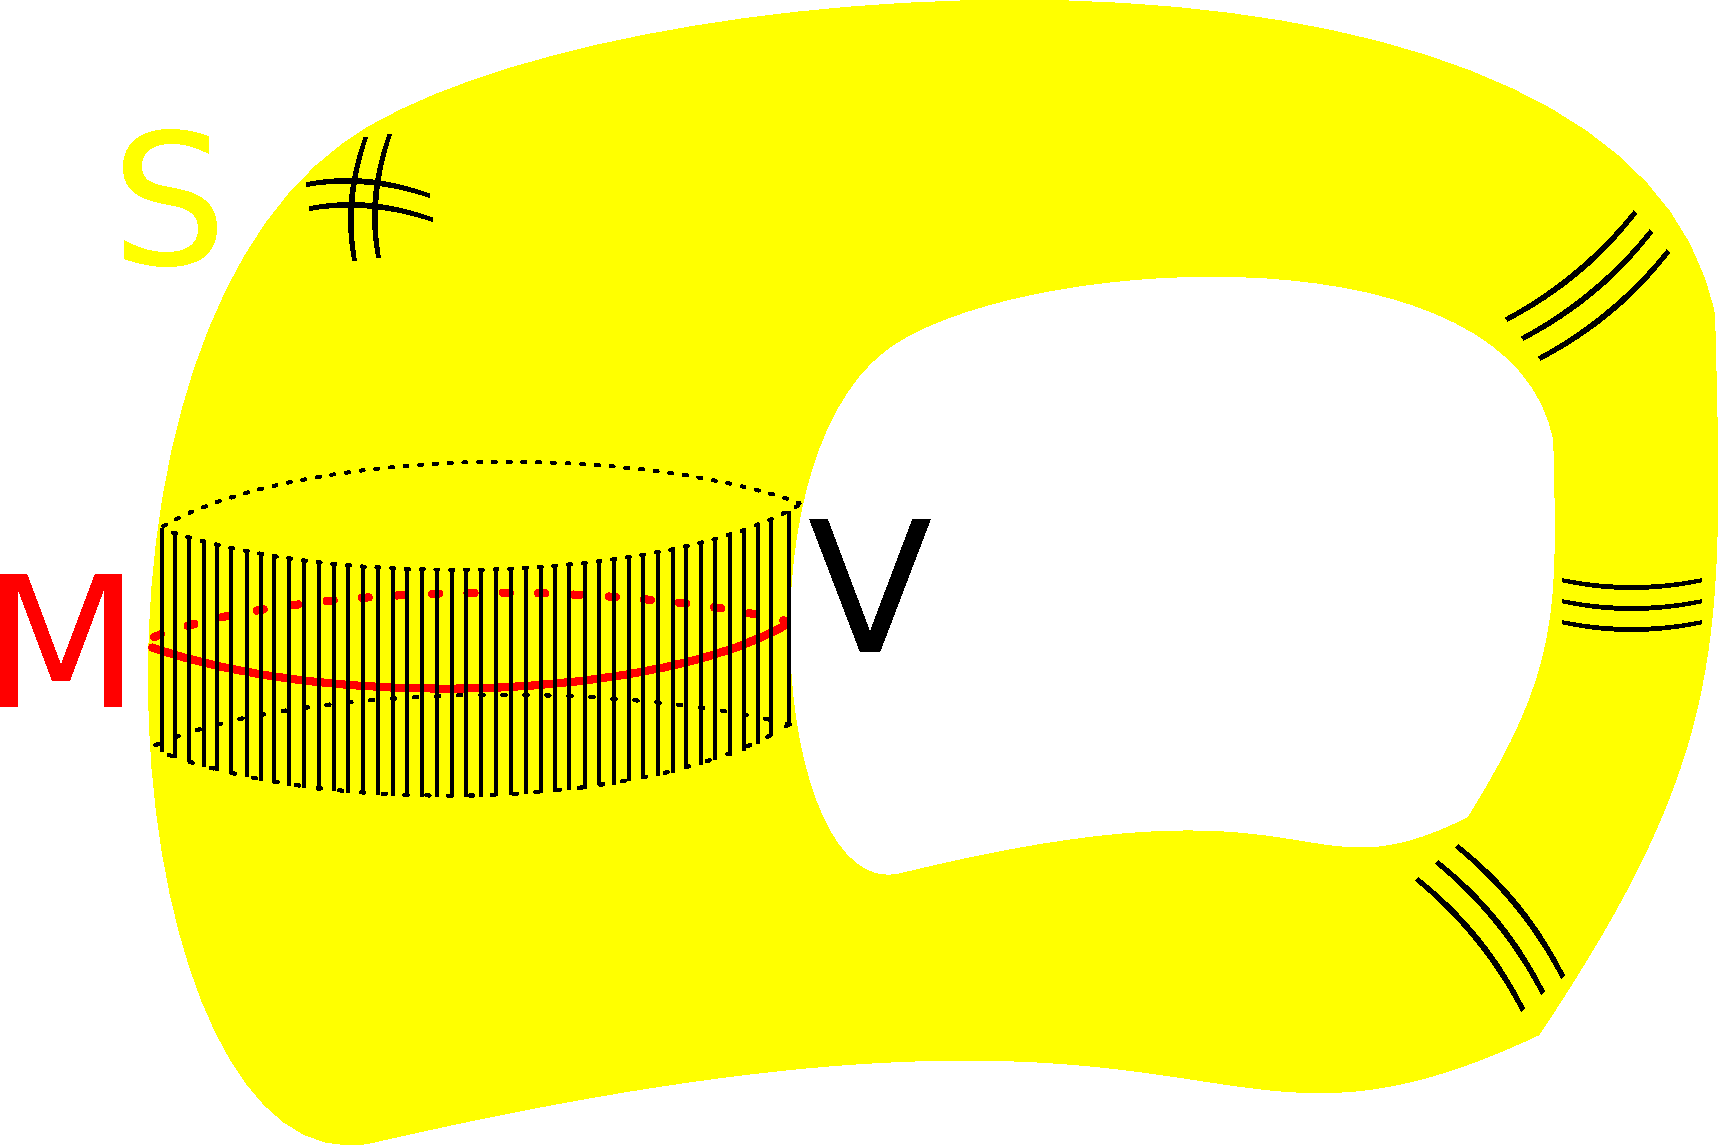
\includegraphics[scale=0.25]{viz_tub.pdf}
	\caption{Vizinhança tubular de um mergulho suave.}
\end{figure}

\par Dito isso, a prova de Stong em (\cite{stong}, Lema 7, p. 274) se resume, a grosso modo, em encontrar um diagrama comutativo nas seguintes condições:

$$ \xymatrix @C=0.5cm {
	H^{*}(S;\Z_{2})\tensor H^{*}(S;\Z_{2}) \ar[rr] & & H^{*}(S;\Z_{2}) \\
	& & \\		 
	H^{*}(S;\Z_{2})\tensor H^{*}(S,S-V;\Z_{2}) \ar[uu] \ar[rr] \ar[dd] & & H^{*}(S,S-V;\Z_{2}) \ar[uu] \ar@/^1.5cm/[lldddd] \ar[dddd] \\
	& & \\				
	H^{*}(V;\Z_{2})\tensor H^{*}(V,\partial V;\Z_{2}) \ar[dd] & & \\
	& & \\	
	H^{*}(V,\partial V;\Z_{2}) \ar[rr] & & H^{*}(S;\Z_{2})
} $$

\par Como não existe vizinhança tubular\index{vizinhança tubular} no contexto topológico, conseguimos contornar esse problema utilizando apenas resultados sobre fibrados generalizados a fim de obter um diagrama comutativo parecido com o diagrama mostrado acima e, assim, mostramos que a existência da vizinhança tubular não é essencial para esse resultado e sim certas consequências algébricas de um mergulho local-flat\index{mergulho!local-flat}.

\par Finalmente, temos o:

\begin{teo}\label{ap_wu_8}
	Se $i:M^{m}\hookrightarrow S^{m+k}$ é um mergulho local-flat\index{mergulho!local-flat}, entre variedades topológicas\index{variedade!topológica} fechadas e conexas, com fibrado generalizado normal\index{fibrado!generalizado!normal} trivial\index{fibrado!generalizado!trivial}, então $v(M)=i^{*}(v(S))$.
\end{teo}

\begin{proof}
	
	\
	
	\par Primeiramente, fixemos algumas notações. Denotemos por $(\mathcal{N},\mathcal{N}_{0})=(N,N_{0},q,M)$ o $\R^{k}-$fibrado generalizado normal\index{fibrado!generalizado!normal} do mergulho local-flat\index{mergulho!local-flat} $i$ e as equivalências homotópicas $f:(N,N_{0})\rightleftarrows (M\times\R^{k},M\times (\R^{k}-\{0\})):g$ dadas pela trivialidade de $(\mathcal{N},\mathcal{N}_{0})$. Lembremos também que $f$ e $g$ são aplicações fibradas\index{aplicação!fibrada}, ou seja, $p_{1}\circ f=q$ e $q\circ g=p_{1}$.
	
	\par Considere $c:S\hookrightarrow (S,S-M)$ a inclusão canônica e $\xi:(N,N_{0})\to (S,S-M)$ a aplicação dada por $\xi(\omega)=\omega(1)$, que segundo (\cite{fadell_1}, Teorema 7.5, p. 509) induz isomorfismo no âmbito de $\Z_{2}-$módulos de (co)homologia singular\index{(co)homologia singular}.
	
	\par Deste modo, ficam bem definidos para qualquer inteiro $t\geq 0$ os homomorfismos:
	$$ B=f_{*}\circ (\xi_{*})^{-1}\circ c_{*}:H_{t}(S;\Z_{2})\to H_{t}(M\times (\R^{k},\R^{k}-\{0\});\Z_{2}) $$
	$$ A=c^{*}\circ (\xi^{*})^{-1}\circ f^{*}:H^{t}(M\times (\R^{k},\R^{k}-\{0\});\Z_{2})\to H^{t}(S;\Z_{2}) $$
	
	\par Vale notar que o homomorifmos $A$ é o dual cohomológico do homomorfismo $B$.
	
	\par Ainda, também sabemos que a fórmula de Künneth\index{fórmula!de Künneth} garante que:
	$$ H^{t+k}(M\times (\R^{k},\R^{k}-\{0\});\Z_{2})\cong H^{t}(M;\Z_{2})\tensor H^{k}(\R^{k},\R^{k}-\{0\};\Z_{2}) $$
	
	\par Então ao denotarmos $(\varphi)=H^{k}(\R^{k},\R^{k}-\{0\};\Z_{2})$, fica bem definido o homomorfismo $\overline{i}:H^{t}(M;\Z_{2})\to H^{t+k}(S;\Z_{2})$ dado por $\overline{i}(x)=A(x\times \varphi)$.
	
	\par Fixadas as notações acima, comecemos a demontração.
	
	\par Se denotarmos por $(\sigma)=H_{k}(\R^{k},\R^{k}-\{0\};\Z_{2})$, então $B([S])=[M]\times\sigma$. Para tanto, note que:
	$$ B([S])\in H_{m+k}(M\times (\R^{k},\R^{k}-\{0\});\Z_{2})\cong H_{m}(M;\Z_{2})\tensor H_{k}(\R^{k},\R^{k}-\{0\};\Z_{2})\cong \Z_{2} $$
	
	\par Como $H_{m}(M;\Z_{2})$ e $H_{k}(\R^{k},\R^{k}-\{0\};\Z_{2})$ são unicamente gerados por $[M]$ e $\sigma$, respectivamente, então $H_{m}(M;\Z_{2})\tensor H_{k}(\R^{k},\R^{k}-\{0\};\Z_{2})$ será unicamente gerado por $[M]\tensor\sigma$, isto é, a única classe não nula de $H_{m+k}(M\times (\R^{k},\R^{k}-\{0\});\Z_{2})$ será $[M]\times\sigma$.
	
	\par Com isso, para que $B([S])=[M]\times\sigma$, é suficiente que $B([S])\neq 0$. Por outro lado, como $B=f_{*}\circ (\xi_{*})^{-1}\circ c_{*}$ e $f_{*}$ e $\xi_{*}$ são isomorfismos, então $B([S])\neq 0$ se, e somente se, $c_{*}([S])\neq 0$.
	
	\par Agora, dado $b\in M\subset S$ arbitrário, então a inclusão $j_{b}:S\hookrightarrow (S,S-\{b\})$ pode ser decomposta nas seguintes inclusões:
	$$ \xymatrix @C=0.5cm {
		S \ar@{^(->}[rr]^-{c} && (S,S-M) \ar@{^(->}[rr] && (S,S-\{b\})
	} $$
	
	\par Como $(j_{b})_{*}$ é um isomorfismo\footnote{Ver proposição \ref{orient_local}.}, então $c_{*}$ será um monomorfismo e, assim, $c_{*}([S])\neq 0$ uma vez que $[S]\neq 0$.
	
	\par Logo, $B([S])=[M]\times\sigma$.
	
	\par Feito isso, mostremos que ao definirmos $e=\xi\circ g:M\times (\R^{k},\R^{k}-\{0\})\to (S,S-M)$, o seguinte diagrama será comutativo para todo $t\geq 0$:
	$$ \xymatrix @C=0.5cm {
		H^{m-t}(S;\Z_{2})\tensor H^{t+k}(S;\Z_{2}) \ar[r]^-{\ccup} & H^{m+k}(S;\Z_{2}) \\
		& \\		 
		H^{m-t}(S;\Z_{2})\tensor H^{t+k}(S,S-M;\Z_{2}) \ar[uu]^-{1\times c^{*}} \ar[r]^-{\ccup} \ar[dd]^-{i^{*}\times e^{*}} & H^{m+k}(S,S-M;\Z_{2}) \ar[uu]^-{c^{*}} \ar@/^2cm/[ldddd]^-{e^{*}} \ar[dddd]^-{c^{*}} \\
		& \\				
		H^{m-t}(M\times\R^{k};\Z_{2})\tensor H^{t+k}(M\times (\R^{k},\R^{k}-\{0\});\Z_{2}) \ar[dd]^-{\ccup} & \\
		& \\	
		H^{m+k}(M\times (\R^{k},\R^{k}-\{0\});\Z_{2}) \ar[r]^-{A} & H^{m+k}(S;\Z_{2})
	} $$
	
	\par Mostremos tal comutatividade por partes. Inicialmente, devido as próprias definições dos homomorfismos $A$ e $e^{*}$, fica evidente que $A\circ e^{*}=c^{*}$.
	
	\par Por outro lado, o lema \ref{propriedades_produtos_2} garante que a inclusão $c:S\hookrightarrow (S,S-M)$ tem a propriedade de que $c^{*}(x\ccup y)=x\ccup c^{*}(y)$ para quaisquer $x\in H^{m-t}(S;\Z_{2})$ e $y\in H^{t+k}(S,S-M;\Z_{2})$.
	
	\par Agora, podemos imaginar, sem perda de generalidade, o mergulho $i:M\hookrightarrow S$ tendo como induzida $i^{*}:H^{t}(S;\Z_{2})\to H^{t}(M\times\R^{k};\Z_{2})$, uma vez que $\R^{k}$ é um espaço topológico contrátil. Ainda, podemos tomar tal contração como sendo $M\to M\times \R^{k}$ que associa $b\mapsto (b,0)$.
	
	\par Assim, para que possamos restringir a imagem de $e:M\times(\R^{k},\R^{k}-\{0\})\to (S,S-M)$ para $S$, é necessário que o domínio seja restrito a $M\times \{0\}$. Deste modo, a restrição $e_{|M\times\{0\}}:M\times\{0\}\to S$ se resume ao mergulho $i$, pois fixado $b\in M$, $g(b,0)\in N-N_{0}$ é o caminho em $S$ constante igual a $b\in M$, e assim:\newline
	
	$ \begin{array}{rl}
		e(b,0) \ = & \xi\circ g(b,0) \\
		= & [g(b,0)](1) \\
		= & b \\
		= & i(b)
	\end{array} $\newline
	
	\par Com isso, teremos para quaisquer $x\in H^{m-t}(S;\Z_{2})$ e $y\in H^{t+k}(S,S-M;\Z_{2})$ que $e^{*}(x\ccup y)=i^{*}(x)\ccup e^{*}(y)$.
	
	\par Feito isso, o diagrama mostrado acima é, de fato, comutativo. Ainda, lembrando que $\overline{i}:H^{t}(M;\Z_{2})\to H^{t+k}(S;\Z_{2})$ é o homomorfismo definido por $\overline{i}(x)=A(x\times \varphi)$, em que $(\varphi)=H^{k}(\R^{k},\R^{k}-\{0\};\Z_{2})$, podemos obter para quaisquer $x\in H^{t}(M;\Z_{2})$ e $y\in H^{m-t}(S;\Z_{2})$, que:\newline
	
	$ \begin{array}{rl}
		A(i^{*}(y)\ccup (x\times\varphi)) \ = & y\ccup c^{*}((e^{*})^{-1}(x\times\varphi)) \\
		= & y\ccup A(x\times\varphi) \\
		= & y\ccup \overline{i}(x)
	\end{array} $ \newline
	
	\par Portanto, temos para quaisquer $x\in H^{t}(M;\Z_{2})$ e $y\in H^{m-t}(S;\Z_{2})$ que: \newline
	
	$ \begin{array}{rl}
		<\overline{i}(x)\ccup y,[S]> \ = & <A(i^{*}(y)\ccup (x\times\varphi)),[S]> \\
		= & <i^{*}(y)\ccup (x\times\varphi),B([S])> \\
		= & <i^{*}(y),([M]\times\sigma)\ccap (x\times\varphi)> \\
		= & <i^{*}(y),([M]\ccap x)\times (\sigma\ccap\varphi)> \\
		= & <i^{*}(y),[M]\ccap x> \\
		= & <x\ccup i^{*}(y),[M]>
	\end{array} $ \newline
	
	\par Finalmente, estamos aptos para provar que $i^{*}(v(S))=v(M)$. Para tanto, devido a unicidade das classes de Wu\index{classe!de Wu}, é suficiente mostrar para todo $0\leq t\leq n$ que:
	$$ <i^{*}(v_{t}(S))\ccup x,[M]>=<Sq^{t}(x),[M]>, \ \forall x\in H^{m-t}(M;\Z_{2}) $$
	
	\par Mas antes, note que $Sq^{t}(\varphi)=0$ quando $t>0$, uma vez que $H^{k+t}(\R^{k},\R^{k}-\{0\};\Z_{2})=0$ para $t>0$ e $Sq^{t}(\varphi)\in H^{k+t}(\R^{k},\R^{k}-\{0\};\Z_{2})$. Com isso, obtemos que $Sq^{t}(x\times \varphi)=Sq^{t}(x)\times\varphi$, para qualquer $x\in H^{*}(M;\Z_{2})$.
	
	\par Deste modo, temos para quaisquer $0\leq t\leq m$ e $x\in H^{m-t}(M;\Z_{2})$ que:\newline
	
	$ \begin{array}{rl}
		<i^{*}(v_{t}(S))\ccup x,[M]> \ = & <\overline{i}(x)\ccup v_{t}(S),[S]> \\
		= & <Sq^{t}(\overline{i}(x)),[S]> \\
		= & <Sq^{t}(A(x\times\varphi)),[S]> \\
		= & <A(Sq^{t}(x)\times\varphi),[S]> \\
		= & <\overline{i}(Sq^{t}(x)),[S]> \\
		= & <\overline{i}(Sq^{t}(x))\ccup 1,[S]> \\
		= & <i^{*}(1)\ccup Sq^{t}(x),[M]> \\
		= & <Sq^{t}(x),[M]>
	\end{array} $ \newline
	
	\par Portanto, $i^{*}(v(S))=v(M)$.
	
\end{proof}

\par Assim, concluímos esse capítulo com várias contribuições no contexto de classes características de variedades topológicas. Mais especificamente, apresentamos aplicações referentes as classes de Stiefel-Whitney\index{classe!de Stiefel-Whitney}, de Euler e de Wu de variedades topológicas fechadas.

\par Entre tais contribuições, destacamos:

	\begin{itemize}
		\item uma segunda demonstração da versão topológica da fórmula de Wu\index{fórmula!de Wu}, sendo alguns dos lemas preliminares desenvolvidos tanto para $\Z_{2}-$módulos, quanto para $\Z-$módulos de (co)homologia singular\index{(co)homologia singular};
		\item como os lemas preliminares da fórmula de Wu nos permitiram relacionar a classe e a característica de Euler\index{classe!de Euler} de uma variedade topológica e, consequentemente, garantir a nulidade da característica de Euler de uma variedade topológica de dimensão ímpar;
		\item uma demonstração alternativa de uma das direções da versão topológica do teorema de Poincaré-Hopf\index{teorema!de Poincaré-Hopf}, o qual mostra a relação entre a existência de um campo de caminhos não singulares\index{campo!de caminhos!não singulares} de uma variedade topológica com a nulidade de sua característica de Euler\index{característica de Euler}, utilizando em sua demonstração a classe de Euler;
		\item como a teoria de fibrados generalizados foi essencial para relacionarmos as classes de Wu\index{classe!de Wu} de variedades topológicas por meio de um mergulho local-flat\index{mergulho!local-flat} com fibrado generalizado normal trivial\index{fibrado!generalizado!normal}\index{fibrado!generalizado!trivial}.
	\end{itemize}

\par Ainda, com todos os resultados até aqui apresentados, também concluímos a importância dos fibrados generalizados\index{fibrado!generalizado} não só como uma ferramenta para a teoria de classes características de variedades topológicas\index{variedade!topológica}, mas como uma teoria em si.





% ---------------------------------------------------------------------------------------------------
% ---------------------------------------------------------------------------------------------------
% ----------------------------------------------------------------------   FÓRMULA DE WU GENERALIZADA
% ---------------------------------------------------------------------------------------------------
% ---------------------------------------------------------------------------------------------------





\chapter{Classes Características de Variedades Generalizadas}\label{cap_wu_gen}
\thispagestyle{empty}

\

\par Nesse capítulo, será apresentado pela primeira vez na literatura uma prova da fórmula de Wu para o contexto de variedades generalizadas\index{variedade!generalizada}.

\par Inicialmente, faremos na seção \ref{sec_varied_gen} um breve resumo, baseado em \cite{biasi}, \cite{denise} e \cite{bredon_2}, sobre o conceito de variedades generalizadas, apresentando a definição de tal objeto bem como algumas de suas propriedades.

\par Construiremos algebricamente na seção \ref{sec_thom_gen} a classe e o isomorfismo de Thom associados a um mergulho entre variedades generalizadas com codimensão específica, sendo tal construção baseada nos resultados apresentados por Dold em (\cite{dold}, Capítulo 8).

\par Já na seção \ref{sec_SW_gen}, construiremos as classes de Stiefel-Whitney\index{classe!de Stiefel-Whitney} de mergulhos entre variedades generalizadas com codimensão específica, as classes de Stiefel-Whitney de variedades generalizadas e também mostraremos qual a semelhança dessas construções com o contexto topológico apresentado no capítulo \ref{cap_clas_carac}.

\par E para encerrarmos o capítulo, apresentaremos na seção \ref{sec_form_wu_gen} a demonstração da fórmula de Wu para variedades generalizadas utilizando apenas suas dualidades, ou seja, sem necessariamente a existência de um fibrado tangente para tais variedades, cujas técnicas utilizadas foram baseadas nos resultados apresentados por Bredon em (\cite{bredon}, Capítulo 6).



% ------------------------------------------------------------------------------------------
% ------------------------------------------------------------------------------------------
% ------------------------------------------------------------------------------------------



\section{Variedades Generalizadas}\label{sec_varied_gen}

\

\par Essa seção tem como objetivo principal apresentar os resultados básicos sobre variedades generalizadas, bem como a definição formal de tais objetos.

\par Para uma leitura mais detalhada sobre variedades generalizadas, ver \cite{biasi}, \cite{bredon_2}, \cite{mio_1}, \cite{mio_2}, \cite{denise}  e \cite{wilder}.

\par Começaremos o capítulo final desse trabalho com as seguintes definições:

\begin{defi}{\bf (Dimensão Cohomológica)\index{dimensão cohomológica}}\label{defi_dim_coh}
	Seja $M$ um espaço topológico localmente compacto e de Hausdorff. Dizemos que $M$ tem $\Z_{2}-$dimensão cohomológica finita, que denotaremos por $dim_{\Z_{2}}M<\infty$\index{dim$_{\Z_{2}}<\infty$}, se existir um inteiro $m\geq 0$ tal que $H^{m+1}_{c}(U;\Z_{2})=0$ para toda vizinhança aberta $U\subset M$.
\end{defi}

\par A definição \ref{defi_dim_coh} é, na verdade, uma consequência sobre a dimensão cohomológica de um espaço, cuja demonstração pode ser encontrada em (\cite{bredon_2}, Teorema 16,14, p. 115).

\begin{defi}{\bf (Variedade Homológica)\index{variedade!homológica}}
	Dizemos que um espaço topológico localmente compacto e de Hausdorff $M$ é uma $m-$variedade $\Z_{2}-$homológica se:
	\begin{itemize}
		\item $dim_{\Z_{2}}M<\infty$;
		\item $\forall b\in M, \ H_{k}(M,M-\{b\};\Z_{2})\cong \left\{ \begin{array}{cl}
			\Z_{2} & , \ se \ k=m \\
			0 & , \ se \ k\neq m
		\end{array}\right.$
	\end{itemize}
\end{defi}

\begin{defi}{\bf (Hereditariamente Paracompacto)\index{hereditariamente paracompacto}}
Chamamos um espaço topológico de Hausdorff $M$ de hereditariamente paracompacto se toda vizinhança aberta de $M$ é paracompacta.
\end{defi} 

\par Em particular, todo espaço métrico é hereditariamente paracompacto\footnote{Para mais detalhes sobre espaços hereditariamente paracompactos, ver (\cite{bredon_2}, Capítulo 1, Seção 6).}.

\begin{defi}{\bf (Localmente Homologicamente Conexo)\index{localmente homologicamente conexo}}
Dizemos que um espaço topológico $M$ é localmente homologicamente conexo, que denotaremos por $HLC_{\Z_{2}}^{\infty}$\index{HLC$_{\Z_{2}}^{\infty}$}, se para qualquer $b\in M$ e qualquer vizinhança aberta $U\subset M$ de $b$, existir uma vizinhança aberta $V\subset U$ também de $b$ tal que o homomorfismo $\wt{H}_{k}(V;\Z_{2})\to \wt{H}_{k}(U;\Z_{2})$ induzido pela inclusão $V\hookrightarrow U$ é trivial para todo inteiro $k\geq 0$.
\end{defi}

\begin{defi}{\bf (Variedade Generalizada)\index{variedade!generalizada}}
Dizemos que um espaço topológico localmente compacto e de Hausdorff $M$ é uma $m$-variedade $\Z_{2}-$generalizada se:
	\begin{enumerate}
		\item $M$ for uma $m-$variedade $\Z_{2}-$homológica;
		\item $M$ for hereditariamente paracompacto;
		\item $M$ for $HLC_{\Z_{2}}^{\infty}$.
	\end{enumerate}
\end{defi}

\par Note que as definições acima podem ser feitas para um coeficiente arbitrário e não necessariamente $\Z_{2}$, mas como o intuito desse capítulo é trabalhar com classes de Stiefel-Whitney e de Wu, então não nos preocuparemos com as variedades que não sejam $\Z_{2}-$generalizadas.

\par Por outro lado, mesmo que a definição de uma variedade generalizada seja de certa forma complexa, essas variedades são bem controlados no ponto de vista algébrico, como veremos adiante.

\par Primeiramente, a dimensão de uma variedade generalizada coincide com sua dimensão cohomológica, como podemos ver na proposição abaixo e cuja demonstração se encontra em (\cite{bredon_2}, Observação 9.6, p. 331).

\begin{prop}
Se $M^{m}$ é uma variedade $\Z_{2}-$generalizada, então $dim_{\Z_{2}}M=m$.
\end{prop}

\par Ainda, os módulos de cohomologia singular das variedades generalizadas são bem comportados no seguinte sentido:

\begin{prop}
Se $M^{m}$ é uma variedade $\Z_{2}-$generalizada compacta, então $H^{k}(M;\Z_{2})$ será um módulo finitamente gerado para todo inteiro $0\leq k\leq m$.
\end{prop}

\par A prova da proposição acima pode ser encontrada em (\cite{bredon_2}, Corolário 17.7, p. 129).

\par A título de curiosidade, as variedades generalizadas se diferenciam das variedades topológicas a partir da dimensão três, como podemos ver no teorema abaixo, cuja prova se encontra em (\cite{bredon_2}, Teorema 16.32, p. 388).

\begin{teo}
Seja $M^{m}$ uma variedade homológica 2º-enumerável\footnote{Um espaço topológico é dito 2º-enumerável se possuir uma base enumerável.} e $m\leq 2$, então $M$ será uma variedade topológica.
\end{teo}

\par Antes de prosseguirmos, queremos destacar que existem diversos estudos referentes a existência de variedades generalizadas que não sejam variedades topológicas. Inclusive, existem condições específicas que garantem quando uma variedade generalizada possui o mesmo tipo de homotopia, ou não, de uma variedade topológica. Mas, como não seguiremos esse caminho e caso o leitor tenha se interessado sobre o assunto, sugerimos \cite{mio_1}, \cite{mio_2} e \cite{gm-book}.

\par Dando sequência ao nosso resumo sobre variedades generalizadas, o próximo resultado garante a existência da dualidade de Poincaré para o contexto dessas variedades, como podemos encontrar em (\cite{bredon_2}, Corolário 10.2, p. 338) e cujo enunciado é idêntico para variedades suaves e topológicas:

\begin{teo}
Sejam $M^{m}$ uma variedade generalizada compacta e conexa e o gerador $([M])=H^{m}(M;\Z_{2})\cong\Z_{2}$. Então, o homomorfismo $\mathcal{D}_{M}:H^{k}(M;\Z_{2})\to H_{m-k}(M;\Z_{2})$ dado por $\mathcal{D}_{M}(x)=[M]\ccap x$ é, de fato, um isomorfismo para todo $k\geq 0$.
\end{teo}

\par Agora, de forma mais geral, Halverson provou em (\cite{halverson}, Teorema 5.2, p. 242) que a dualidade de Poincaré-Hopf também é válida para variedades generalizadas, em que podemos considerar o seguinte enunciado:

\begin{teo}
Sejam $N^{n}$ uma variedade generalizada compacta, $M\subset N$ um subespaço fechado e o gerador $([N]_{M})=H_{n}(N,N-M;\Z_{2})\cong\Z_{2}$. Deste modo, o homomorfismo $\mathcal{D}_{N,M}:\check{H}^{k}(M;\Z_{2})\to H_{n-k}(N,N-M;\Z_{2})$ dado por $\mathcal{D}_{N,M}(x)=[N]_{M}\ccap x$ é, de fato, um isomorfismo para todo $k\geq 0$.
\end{teo}

\par Após essas considerações iniciais sobre variedades generalizadas, podemos assumir que esses objetos são, a grosso modo, espaços topológicos que possuem o mesmo comportamento de variedades topológicas no âmbito de $\Z_{2}-$módulos de (co)homologia singular.

\par Ainda, devido a algumas técnicas que utilizaremos no decorrer do capítulo, iremos trabalhar a partir de agora com uma classe particular, mas ainda ampla, de variedades generalizadas, que são as ENR-variedades homológicas\footnote{A condição de ENR é suficiente para garantir que uma variedade homológica seja uma variedade generalizada.}. A fim de ilustrarmos brevemente essa classe de variedades que utilizaremos nesses capítulo, veremos a seguir um exemplo de uma ENR-variedade homológica que não é homeomorfa a uma variedade topológica.

\begin{ex}
Seja $M^{m}$ uma variedade topológica não homeomorfa à esfera $\mathbb{S}^{m}$, mas que é uma $(\Z_{2},m)-$esfera de homologia, ou seja, $H_{k}(M;\Z_{2})\cong H_{k}(\mathbb{S}^{m};\Z_{2})$ para todo inteiro $k\geq 0$. Então, a suspensão $S(M)$ de $M$ será uma ENR-variedade homológica de dimensão $m+1$.

\par De fato, como $M$ é um espaço ENR, então a suspensão $S(M)$ também será um ENR. Por outro lado, sabemos que $H_{k}(S(M),S(M)-\{b\};\Z_{2})\cong H_{k}(\R^{m+1},\R^{m+1}-\{0\};\Z_{2})$  para quaisquer $b\in S(M)$ e $k\geq 0$ inteiro, isto é, $S(M)$ é uma variedade homológica.

\par Entretanto, $S(M)$ não é uma variedade topológica, pois dada qualquer vizinhança aberta $V\subset S(M)$ do vértice superior $v_{+}\in S(M)$ da suspensão $S(M)$, também sabemos que $V\approx C_{+}(M)$ em que $C_{+}(M)$ é o cone superior da suspensão $S(M)$, porém $C_{+}(M)$ não homeomorfo ao disco $D^{m+1}$, uma vez que o bordo $\partial(C_{+}(M))=M$ não é homeomorfo à esfera $\mathbb{S}^{m}$.
\end{ex}

\par O exemplo acima foi retirado de (\cite{denise}, Exemplo 2.2.4, p. 23).



% ------------------------------------------------------------------------------------------
% ------------------------------------------------------------------------------------------
% ------------------------------------------------------------------------------------------



\section{Classe e Isomorfismo de Thom}\label{sec_thom_gen}

\

\par Em (\cite{dold}, Capítulo 8), Dold construiu a classe e o isomorfismo de Thom associados a um mergulho entre variedades topológicas utilizando as dualidades de Poincaré e Poincaré-Lefschetz. Após estudarmos mais atenciosamente essas construções, percebemos que Dold utilizou apenas propriedades algébricas das variedades topológicas, nos motivando a tentar fazer o mesmo para o contexto de variedades generalizadas\index{variedade!generalizada}.

\par Feitas algumas adaptações nos resultados apresentados por Dold, veremos nessa seção como construir algebricamente a classe\index{classe!de Thom} e o isomorfismo de Thom\index{isomorfismo!de Thom} associados a um mergulho topológico\index{mergulho!topológico}, com codimensão específica, entre ENR\index{ENR}-variedades homológicas\index{variedade!homológica} utilizando apenas as dualidades de Poincaré\index{dualidade!de Poincaré} e Poincaré-Lefschetz\index{dualidade!de Poincaré-Lefschetz} dessas variedades.

\par Para tanto, vamos fixar ao longo dessa seção as seguintes condições:

	\begin{itemize}
		\item $s:M^{m}\to N^{2m}$ será um mergulho topológico\index{mergulho!topológico} entre ENR\index{ENR}-variedades homológicas\index{variedade!homológica} compactas e conexas;
		\item como podemos considerar, sem perda de generalidade, que $M\subset N$, então vamos supor que $M$ é um retrato\index{retrato} de $N$, ou seja, vamos supor que exista uma aplicação $p:N^{2m}\to M^{m}$ tal que $p\circ s=1$;
		\item $\mathcal{D}_{M}:H^{k}(M;\Z_{2})\to H_{m-k}(M;\Z_{2})$ será a dualidade de Poincaré\index{dualidade!de Poincaré} de $M$, que é definida por $\mathcal{D}_{M}(x)=[M]\ccap x$;
		\item $\mathcal{D}_{N}:H^{k}(N;\Z_{2})\to H_{2m-k}(N;\Z_{2})$ será a dualidade de Poincaré\index{dualidade!de Poincaré} de $N$, que é definida por $\mathcal{D}_{N}(x)=[N]\ccap x$;
		\item $\mathcal{D}_{N,M}:H^{k}(M;\Z_{2})\to H_{2m-k}(N,N-M;\Z_{2})$ será a dualidade de Poincaré-Lefschetz\index{dualidade!de Poincaré-Lefschetz} de $M\subset N$, que é definida por $\mathcal{D}_{N,M}(x)=[N]_{M}\ccap x$.
	\end{itemize}

\par Antes de prosseguirmos, recordemos que como toda variedade homológica é $\Z_{2}-$orientável, então nada nos impede de considerarmos as dualidades citadas acima, lembrando que as classes de orientação global\index{classe!de orientação global} de $M$ e $N$ são, respectivamente, os geradores $([M])=H_{m}(M;\Z_{2})$ e $([N])=H_{2m}(N;\Z_{2})$ e a classe de orientação local\index{classe!de orientação local} de $N$ ao longo de $M$ é o gerador $([N]_{M})=H_{2m}(N,N-M;\Z_{2})$.

\par Ainda, ao fixarmos a inclusão canônica $j:N\hookrightarrow (N,N-M)$, também sabemos que as dualidades $\mathcal{D}_{N}$ e $\mathcal{D}_{N,M}$ se relacionam por meio do seguinte diagrama comutativo:
$$ \xymatrix @C=0.5cm {
	H^{k}(N;\Z_{2}) \ar[rr]^-{s^{*}} \ar[ddd]^-{\mathcal{D}_{N}} \ar[rrddd]^-{[N]_{M}\ccap} && H^{k}(M;\Z_{2}) \ar[ddd]^-{\mathcal{D}_{N,M}} \\
	&& \\
	&& \\
	H_{2m-k}(N;\Z_{2}) \ar[rr]^-{j_{*}} && H_{2m-k}(N,N-M;\Z_{2})
} $$

\par Uma vez que $\mathcal{D}_{N}(1)=[N]$ e o diagrama acima comuta, concluímos a seguinte relação:
$$ j_{*}([N])=[N]_{M} $$

\par Ainda, o diagrama acima também nos garante o seguinte:

\begin{lem}\label{lema_tecnico_dualidades}
	Dado $a\in H_{k}(N,N-M;\Z_{2})$ arbitrário, então existe $x\in H^{2m-k}(N;\Z_{2})$ tal que $a=[N]_{M}\ccap x$
\end{lem}
\begin{proof}
	
	\
	
	\par Segue diretamente da relação $\mathcal{D}_{N,M}\circ s^{*}(\_)=[N]_{M}\ccap(\_)$ e dos fatos que $\mathcal{D}_{N,M}$ é um isomorfismo e $s^{*}$ é sobrejetora, uma vez que $p\circ s=1$.
	
\end{proof}

\par Agora que fixamos todas as notações necessárias para o desenvolvimento do restante deste capítulo, vejamos como construir a classe de Thom\index{classe!de Thom} associada ao mergulho $s:M^{m}\to N^{2m}$. Para tanto, comecemos definindo o isomorfismo transfer:

\begin{defi}{\bf (Isomorfismo Transfer\index{isomorfismo!transfer})}
	Chamaremos de isomorfismo transfer associado ao mergulho $s:M^{m}\to N^{2m}$ o homomorfismo $s_{!}:H_{k}(N,N-M;\Z_{2})\to H_{k-m}(M;\Z_{2})$ dado pela seguinte composição de isomorfismos:
		$$ \xymatrix @C=0.5cm {
		s_{!}:H_{k}(N,N-M;\Z_{2}) \ar[rrr]^-{\mathcal{D}^{-1}_{N,M}} &&& H^{2m-k}(M;\Z_{2}) \ar[rrr]^-{\mathcal{D}_{M}} &&& H_{k-m}(M;\Z_{2})
		} $$
\end{defi}

\par Devido ao isomorfismo transfer, temos que: \newline

$H_{k}(N,N-M;\Z_{2}) \ \cong \ \left\{\begin{array}{cl}
	\Z_{2} & , \ k=m \mbox{ e } k=2m \\
	0      & , \ k<m \mbox{ ou } k>2m
\end{array}\right.$ \newline

\par Com isso, o teorema dos Coeficientes Universais\index{teorema!dos Coeficientes Universais} nos garante que: \newline

$H^{k}(N,N-M;\Z_{2}) \ \cong \ \left\{\begin{array}{cl}
	\Z_{2} & , \ k=m \mbox{ e } k=2m \\
	0      & , \ k<m \mbox{ ou } k>2m
\end{array}\right.$ \newline

\begin{defi}{\bf (Classe de Thom\index{classe!de Thom})}
	Chamamos de classe de Thom associada ao mergulho $s:M^{m}\to N^{2m}$ o gerador $(\tau_{s})=H^{m}(N,N-M;\Z_{2})$
\end{defi}

\par Vejamos também que o isomorfismo transfer\index{isomorfismo!transfer} $s_{!}$ e o mergulho $s$ se relacionam da seguinte maneira:

\begin{lem}\label{lema_tecnico_dualidades_4}
	Para qualquer $x\in H^{k}(N;\Z_{2})$, temos que:
	$$ s_{!}([N]_{M}\ccap x)=[M]\ccap s^{*}(x) $$
\end{lem}
\begin{proof}
	
	\
	
	\par Dado $x\in H^{k}(N;\Z_{2})$ qualquer e lembrando que $\mathcal{D}_{N,M}\circ s^{*}(x)=[N]_{M}\ccap x$, concluímos: \newline
	
	$ \begin{array}{rl}
		s_{!}([N]_{M}\ccap x) \ = & s_{!}\circ \mathcal{D}_{N,M}\circ s^{*}(x) \\
		= & \mathcal{D}_{M}\circ \mathcal{D}_{N,M}^{-1}\circ \mathcal{D}_{N,M}\circ s^{*}(x) \\
		= & \mathcal{D}_{M}\circ s^{*}(x) \\
		= & [M]\ccap s^{*}(x)
	\end{array} $
	
\end{proof}

\par Agora, os dois lemas a seguir nos garantirão em $H^{m}(N;\Z_{2})$ um representante da classe de Thom\index{classe!de Thom} $\tau_{s}\in H^{m}(N,N-M;\Z_{2})$ associada ao mergulho $s:M^{m}\to N^{2m}$.

\begin{lem}\label{lema_tecnico_dualidades_3}
	Existe uma única classe não-nula $U_{s}\in H^{m}(N;\Z_{2})$ de modo que:
	$$ s_{*}([M])=[N]\ccap U_{s} $$
\end{lem}
\begin{proof}
	
	\
	
	\par Inicialmente, como $[M]\neq 0$ em $H_{m}(M;\Z_{2})$ e $s_{*}$ é injetora, uma vez que $p\circ s=1$, então $s_{*}([M])\neq 0$ em $H_{m}(N;\Z_{2})$.
	
	\par Sendo $\mathcal{D}_{N}:H^{m}(N;\Z_{2})\to H_{m}(N;\Z_{2})$ um isomorfismo, então existirá uma única classe não-nula $U_{s}\in H^{m}(N;\Z_{2})$ tal que $\mathcal{D}_{N}(U_{s})=s_{*}([M])$, ou seja, $[N]\ccap U_{s}=s_{*}([M])$.
	
\end{proof}

\begin{prop}\label{principal}
	A inclusão canônica $j:N\hookrightarrow (N,N-M)$ é tal que:
	$$ j^{*}(\tau_{s})=U_{s} $$
\end{prop}
\begin{proof}
	
	\
	
	\par Inicialmente, como $U_{s}\neq 0$ em $H^{m}(N;\Z_{2})$ e $\tau_{s}\neq 0$ em $H^{m}(N,N-M;\Z_{2})$, então teremos que $\tau_{s}\ccup\tau_{s}\neq 0$ e $U_{s}\ccup\tau_{s}\neq 0$, ambos em $H^{2m}(N,N-M;\Z_{2})$. Deste modo, como $H^{2m}(N,N-M;\Z_{2})\cong\Z_{2}$, então:
	$$ (\tau_{s}\ccup\tau_{s})=H^{2m}(N,N-M;\Z_{2})=(U_{s}\ccup\tau_{s}) $$
	
	\par Ainda, como $([N]_{M})=H_{2m}(N,N-M;\Z_{2})\cong\Z_{2}$, então:
	$$ <\tau_{s}\ccup\tau_{s},[N]_{M}> \ = \ 1 \ = \ <U_{s}\ccup\tau_{s},[N]_{M}> $$
	
	\par Agora, vamos garantir que $j^{*}(\tau_{s})\neq 0$. Para tanto, note que: \newline
	
	$\begin{array}{rl}
		<j^{*}(\tau_{s}),[N]_{M}\ccap \tau_{s}> \ = & <j^{*}(\tau_{s})\ccup\tau_{s},[N]_{M}> \\
		= & <j^{*}(\tau_{s})\ccup\tau_{s},j_{*}([N])> \\
		= & <j^{*}(j^{*}(\tau_{s})\ccup\tau_{s}),[N]> \\
		= & <j^{*}(\tau_{s})\ccup j^{*}(\tau_{s}),[N]> \\
		= & <j^{*}(\tau_{s}\ccup\tau_{s}),[N]> \\
		= & <\tau_{s}\ccup\tau_{s},j_{*}([N])> \\
		= & <\tau_{s}\ccup\tau_{s},[N]_{M}> \\
		= & 1
	\end{array}$\newline
	
	\par Por outro lado, caso $j^{*}(\tau_{s})=0$, então teríamos que $<j^{*}(\tau_{s}),[N]_{M}\ccap \tau_{s}>=0$, o que seria um absurdo. Assim, $j^{*}(\tau_{s})\neq 0$.
	
	\par Com isso, como $j^{*}(\tau_{s})\neq 0$, então a proposição \ref{prop_alg_comut} nos garantirá que existe uma única classe $x\in H^{m}(N;\Z_{2})$ tal que $x\neq 0$ e $<x,\mathcal{D}_{N}(j^{*}(\tau_{s}))>=1$. Se provarmos que $<U_{s},\mathcal{D}_{N}(j^{*}(\tau_{s}))>=1=<j^{*}(\tau_{s}),\mathcal{D}_{N}(j^{*}(\tau_{s}))>$, então concluiremos por unicidade que $j^{*}(\tau_{s})=U_{s}$. Façamos isso: \newline
	
	$\begin{array}{rl}
		<U_{s},\mathcal{D}_{N}(j^{*}(\tau_{s}))> \ = & <U_{s},[N]\ccap j^{*}(\tau_{s})> \\
		= & <U_{s}\ccup j^{*}(\tau_{s}),[N]> \\
		= & <j^{*}(U_{s}\ccup\tau_{s}),[N]> \\
		= & <U_{s}\ccup\tau_{s},j_{*}([N])> \\
		= & <U_{s}\ccup\tau_{s},[N]_{M}> \\
		= & 1
	\end{array}$ \newline
	
	\par Por outro lado: \newline
	
	$\begin{array}{rl}
		<j^{*}(\tau_{s}),\mathcal{D}_{N}(j^{*}(\tau_{s}))> \ = & <j^{*}(\tau_{s}),[N]\ccap j^{*}(\tau_{s})> \\
		= & <j^{*}(\tau_{s})\ccup j^{*}(\tau_{s}),[N]> \\
		= & <j^{*}(\tau_{s}\ccup\tau_{s}),[N]> \\
		= & <\tau_{s}\ccup\tau_{s},j_{*}([N])> \\
		= & <\tau_{s}\ccup\tau_{s},[N]_{M}> \\
		= & 1
	\end{array}$ \newline
	
	\par Portanto, $j^{*}(\tau_{s})=U_{s}$.
	
\end{proof}

\par Assim, precisamos mostrar apenas mais alguns resultados técnicos sobre a classe de Thom\index{classe!de Thom} para finalmente podermos definir o isomorfismo de Thom.

\begin{lem}\label{lema_tecnico_dualidades_2}
	$s_{*}([M])=[N]_{M}\ccap \tau_{s}$
\end{lem}
\begin{proof}
	
	\
	
	\par Basta combinar o lema \ref{lema_tecnico_dualidades_3}, a proposição \ref{principal} e o lema \ref{propriedades_produtos_3} da seguinte forma:\newline
	
	$ \begin{array}{rl}
		s_{*}([M]) \ = & [N]\ccap U_{s} \\
		= & [N]\ccap j^{*}(\tau_{s}) \\
		= & j_{*}([N])\ccap\tau_{s} \\
		= & [N]_{M}\ccap \tau_{s}
	\end{array} $
	
\end{proof}

\begin{prop}
	Para qualquer $a\in H_{k}(N,N-M;\Z_{2})$, temos:
	$$ s_{*}\circ s_{!}(a)=a\ccap\tau_{s} $$
\end{prop}
\begin{proof}
	
	\
	
	\par Primeiramente, sabemos pelo lema \ref{lema_tecnico_dualidades} que dado $a\in H_{k}(N,N-M;\Z_{2})$ qualquer, existe $x\in H^{2m-k}(N;\Z_{2})$ tal que $a=[N]_{M}\ccap x$.
	
	\par Deste modo, os lemas \ref{lema_tecnico_dualidades_4} e \ref{lema_tecnico_dualidades_2} nos garantem que: \newline
	
	$ \begin{array}{rl}
		s_{*}\circ s_{!}(a) \ = & s_{*}\circ s_{!}([N]_{M}\ccap x) \\
		= & s_{*}([M]\ccap s^{*}(x)) \\
		= & s_{*}([M])\ccap x \\
		= & \left( [N]_{M}\ccap \tau_{s} \right)\ccap x \\
		= & [N]_{M}\ccap \left( \tau_{s}\ccup x \right) \\
		= & [N]_{M}\ccap \left( x\ccup \tau_{s} \right) \\
		= & \left( [N]_{M}\ccap x \right)\ccap \tau_{s} \\
		= & a\ccap\tau_{s}
	\end{array} $
	
\end{proof}

\begin{teo}
	O isomorfismo transfer\index{isomorfismo!transfer} $s_{!}:H_{k}(N,N-M;\Z_{2})\to H_{k-m}(M;\Z_{2})$ pode ser decomposto da seguinte maneira:
	$$ \xymatrix @C=0.5cm {
		s_{!}:H_{k}(N,N-M;\Z_{2}) \ar[rr]^-{\ccap \tau_{s}} && H_{k-m}(N;\Z_{2}) \ar[rr]^-{p_{*}} && H_{k-m}(M;\Z_{2})
	} $$
\end{teo}
\begin{proof}
	
	\
	
	\par Dado $a\in H_{k}(N,N-M;\Z_{2})$ qualquer e lembrando que $p\circ s=1$, então a proposição anterior nos garantirá que:\newline
	
	$ \begin{array}{rl}
		p_{*}(a\ccap\tau_{s}) \ = & p_{*}\circ s_{*}\circ s_{!}(a) \\
		= & s_{!}(a)
	\end{array} $
	
\end{proof}

\begin{teo}{\bf (Isomorfismo de Thom\index{isomorfismo!de Thom})}\label{iso_thom_vg}
	Para qualquer inteiro $k\geq 0$, a seguinte composição será um isomorfismo:
	$$ \xymatrix @C=0.5cm {
		\phi_{s}:H^{k}(M;\Z_{2}) \ar[rr]^-{p^{*}} && H^{k}(N;\Z_{2}) \ar[rr]^-{\ccup \tau_{s}} && H^{k+m}(N,N-M;\Z_{2})
	} $$
\end{teo}

\begin{proof}
	
	\
	
	\par Primeiramente, note que para quaisquer $a\in H_{k+m}(N,N-M;\Z_{2})$ e $x\in H^{k}(M;\Z_{2})$, temos que: \newline
	
	$ \begin{array}{rl}
		<\phi_{s}(x),a> \ = & <p^{*}(x)\ccup\tau_{s},a> \\
		= & <p^{*}(x),a\ccap\tau_{s}> \\
		= & <x,p_{*}(a\ccap\tau_{s})> \\
		= & <x,s_{!}(a)>
	\end{array} $\newline
	
	\par Deste modo, $\phi_{s}$ é o dual cohomológico de $s_{!}$ e, uma vez que $s_{!}$ é um isomorfismo, então o teorema dos Coeficientes Universais\index{teorema!dos Coeficientes Universais} garantirá que $\phi_{s}$ será um isomorfismo.
	
\end{proof}

\begin{defi}
	Chamamos o isomorfismo $\phi_{s}:H^{k}(M;\Z_{2})\to H^{k+m}(N,N-M;\Z_{2})$ dado no teorema \ref{iso_thom_vg} de isomorfismo de Thom\index{isomorfismo!de Thom} associado ao mergulho $s:M^{m}\to N^{2m}$.
\end{defi}



% ------------------------------------------------------------------------------------------
% ------------------------------------------------------------------------------------------
% ------------------------------------------------------------------------------------------



\section{Classes de Stiefel-Whitney}\label{sec_SW_gen}

\

\par Construiremos nessa seção, de forma totalmente algébrica, as classes de Stiefel-Whitney\index{classe!de Stiefel-Whitney} de mergulhos entre variedades homológicas\index{variedade!homológica} e as classes de Stiefel-Whitney de variedades homológicas. Ainda, utilizando resultados técnicos obtidos por Fadell em \cite{fadell_1}, mostraremos algumas semelhanças dessas construções com as classes de Stiefel-Whitney dos fibrados generalizados normais\index{fibrado!generalizado!normal} de mergulhos local-flat\index{mergulho!local-flat} e as classes de Stiefel-Whitney de variedades topológicas apresentadas no capítulo \ref{cap_clas_carac}.

\par Inicialmente, como podemos associar a cada mergulho topológico\index{mergulho!topológico} entre variedades homológicas\index{variedade!homológica}, sobre condições específicas, a sua classe\index{classe!de Thom} e o seu isomorfismo\index{isomorfismo!de Thom} de Thom, é possível definir as classes de Stiefel-Whitney\index{classe!de Stiefel-Whitney} desse mergulho de modo análogo ao que foi feito para fibrados vetoriais\index{fibrado!vetorial} em (\cite{milnor_1}, Capítulo 4) e para fibrados generalizados\index{fibrado!generalizado} no capítulo \ref{cap_clas_carac}, da seguinte maneira:

\begin{defi}{\bf (Classes de Stiefel-Whitney)\index{classe!de Stiefel-Whitney}}\label{defi_SW_merg}
Considere $s:M^{m}\to N^{2m}$ um mergulho topológico entre ENR-variedades homológicas compactas e conexas de modo que $M$ seja um retrato\index{retrato} de $N$. Denotando por $\tau_{s}$ e $\phi_{s}$ a classe e o isomorfismo de Thom associados ao mergulho $s$, respectivamente, definimos a $k-$ésima classe de Stiefel-Whitney do mergulho $s$ por:
	$$ w_{k}(s)=\phi_{s}^{-1}\circ Sq^{k}(\tau_{s})\in H^{k}(M;\Z_{2}) $$

\par Ainda, chamamos $W(s)=\ds\sum_{k\geq 0}w_{k}(s)\in H^{*}(M;\Z_{2})$ de classe de Stiefel-Whitney total\index{classe!de Stiefel-Whitney total} de $s$.
\end{defi}

\par Devido as propriedades dos quadrados de Steenrod, o próximo resultado é análogo ao teorema \ref{res_SW_fht_1}.

\begin{prop}
	Se $s:M^{m}\to N^{2m}$ é um mergulho topológico entre ENR-variedades homológicas compactas e conexas de modo que $M$ seja um retrato\index{retrato} de $N$, então $w_{0}(s)=1$ e $w_{k}(s)=0$ para $k>m$. Em outras palavras, $W(s)=1+\ds\sum_{k=1}^{m}w_{k}(s)$.
\end{prop}

\par Agora, como todo mergulho local-flat é um mergulho topológico e toda variedade topológica é uma ENR-variedade homológica, então obtemos o seguinte:

\begin{teo}\label{SW_normal_gen}
Sejam $s:M^{m}\to S^{2m}$ um mergulho local-flat\index{mergulho!local-flat} entre variedades topológicas fechadas e conexas, de modo que $M$ seja um retrato\index{retrato} de $S$, e $(\mathcal{N},\mathcal{N}_{0})$ o seu $\R^{m}-$fibrado generalizado normal\index{fibrado!generalizado!normal}. Denotando por $W(\mathcal{N},\mathcal{N}_{0})$ e $W(s)$ as classes de Stiefel-Whitney totais\index{classe!de Stiefel-Whitney total} dadas pelas definições \ref{defi_SW_top} e \ref{defi_SW_merg}, respectivamente, então $W(\mathcal{N},\mathcal{N}_{0})=W(s)$.
\end{teo}
\begin{proof}

\

\par Inicialmente, lembremos que o $\R^{m}-$fibrado generalizado normal do mergulho local-flat $s:M\to S$ é o par $(\mathcal{N},\mathcal{N}_{0})=(N,N_{0},q,M)$\footnote{Nesse capítulo, a letra $N$ não denotará uma variedade apenas na demonstração do Teorema \ref{SW_normal_gen}.} em que:

	\begin{itemize}
		\item $N_{0}=\{ \omega\in S^{I} \ : \ \omega(t)\in M \Leftrightarrow t=0 \}$
		\item $N=N_{0}\bigcup \{ \omega\in S^{I} \ : \ \omega(t)=\omega(0)\in M, \ \forall t\in I \}$
		\item $q:N\to M$ é dada por $q(\omega)=\omega(0)$
	\end{itemize}

\par Sendo $s:M\to S$ um mergulho local-flat, denotemos por $\tau\in H^{m}(N,N_{0};\Z_{2})$ e $\phi:H^{k}(M;\Z_{2})\to H^{k+m}(N,N_{0};\Z_{2})$ a classe e o isomorfismo de Thom, respectivamente, de $(\mathcal{N},\mathcal{N}_{0})$, em que $\phi(x)=q^{*}(x)\ccup \tau$.

\par Por outro lado, considerando $s:M\to S$ como um mergulho topológico\index{mergulho!topológico} entre ENR\index{ENR}-variedades homológicas compactas e conexas de modo que $M$ seja um retrato de $S$, consideremos $p:S\to M$ tal retração\index{retração} e denotemos por $\tau_{s}\in H^{m}(S,S-M;\Z_{2})$ a classe de Thom\index{classe!de Thom} e $\phi_{s}:H^{k}(M;\Z_{2})\to H^{k+m}(S,S-M;\Z_{2})$ o isomorfismo de Thom\index{isomorfismo!de Thom}, ambos associados ao mergulho $s$, em que $\phi_{s}(x)=p^{*}(x)\ccup\tau_{s}$.

\par Agora, definindo $\xi:(N,N_{0})\to (S,S-M)$ por $\xi(\omega)=\omega(1)$, então (\cite{fadell_1}, Teorema 7.5, p. 509) nos garantirá que $\xi$ induzirá isomorfismo no âmbito de $\Z_{2}-$módulos de cohomologia singular de modo que $\xi^{*}(\tau_{s})=\tau$.

\par Ainda, como $N-N_{0}=\{ \omega\in S^{I} \ : \ \omega(t)=\omega(0)\in M, \ \forall t\in I \}$, então podemos considerar a restrição $\xi_{|N-N_{0}}:(N-N_{0})\to (S-(S-M))$ definida por:\newline

	$\begin{array}{rl}
		\xi_{|N-N_{0}}(\omega) \ = & \omega(1) \\
								 = & \omega(0) \\
								 = & q(\omega)
	\end{array}$\newline

\par Assim, teremos que $\xi^{*}\circ\phi_{s}=\phi$. De fato:\newline

	$\begin{array}{rl}
		\forall k\geq 0, \ \forall x\in H^{k}(M;\Z_{2}), \ \xi^{*}\circ\phi_{s}(x) \ = & \xi^{*}\left( p^{*}(x)\ccup\tau_{s} \right) \\
		 = & q^{*}(x)\ccup\xi^{*}(\tau_{s}) \\
		 = & q^{*}(x)\ccup \tau \\
		 = & \phi(x)
	\end{array}$ \newline

\par Deste modo, o seguinte diagrama será, para qualquer inteiro $k\geq 0$, comutativo:

$$ \xymatrix @C=0.5cm {
	H^{m}(S,S-M;\Z_{2}) \ar[dd]^-{\xi^{*}} \ar[rr]^-{Sq^{k}} && H^{k+m}(S,S-M;\Z_{2}) \ar[dd]^-{\xi^{*}} \ar[rrd]^-{\phi_{s}^{-1}} && \\
	&& && H^{k}(M;\Z_{2}) \\
	H^{m}(N,N_{0};\Z_{2}) \ar[rr]^-{Sq^{k}} && H^{k+m}(N,N_{0};\Z_{2}) \ar[rru]^-{\phi^{-1}} &&
} $$

\par Portanto, temos para todo $k\geq 0$ que: \newline

$ \begin{array}{rl}
	w_{k}(\mathcal{N},\mathcal{N}_{0}) \ = & \phi^{-1}\circ Sq^{k}(\tau) \\
	= & \phi^{-1}\circ Sq^{k}\circ \xi^{*}(\tau_{s}) \\
	= & \phi^{-1}\circ \xi^{*}\circ Sq^{k}(\tau_{s}) \\
	= & \phi_{s}^{-1}\circ Sq^{k}(\tau_{s}) \\
	= & w_{k}(s)
\end{array} $

\end{proof}

\par Veja que, mesmo não existindo uma noção de fibrado tangente para variedades homológicas, é possível definir as classes de Stiefel-Whitney de tais variedades da seguinte maneira:

\begin{defi}{\bf (Classes de Stiefel-Whitney\index{classe!de Stiefel-Whitney})}\label{defi_SW_hom}
Seja $M^{m}$ uma ENR\index{ENR}-variedade homológica\index{variedade!homológica} compacta e conexa. Como a aplicação diagonal\index{aplicação!diagonal} $d:M\to M\times M$ é um mergulho topológico\index{mergulho!topológico} e a projeção canônica $p_{1}:M\times M\to M$ é uma retração\index{retração} de $M\times M$ em $M$, então podemos definir a classe de Stiefel-Whitney total\index{classe!de Stiefel-Whitney total} de $M$ por $W(M)=W(d)$.
\end{defi}

\par Para que a construção das classes de Stiefel-Whitney de uma variedade homológica\index{variedade!homológica} seja, de fato, bem definida, devemos nos atentar ao seguinte ponto: como toda variedade topológica é uma variedade homológica, então a construção das classes de Stiefel-Whitney de uma variedade topológica deve ser a mesma independentemente se utilizarmos a construção dada por Fadell para variedades topológicas\index{variedade!topológica} como na definição \ref{defi_SW_top} ou se utilizarmos nossa construção para variedades generalizadas como na definição \ref{defi_SW_hom}. Em outras palavras:

\begin{teo}\label{SW_tang_gen}
	Considere $M^{m}$ uma variedade topológica fechada e conexa, $(\tau M,\tau_{0}M)$ o seu $\R^{m}-$fibrado generalizado tangente\index{fibrado!generalizado!tangente} e $d:M\to M\times M$ a diagonal\index{aplicação!diagonal}. Denotando por $W(\tau M,\tau_{0}M)$ e $W(d)$ as classes de Stiefel-Whitney totais\index{classe!de Stiefel-Whitney total} de $M$ dadas pelas definições \ref{defi_SW_top} e \ref{defi_SW_hom}, respectivamente, então $W(\tau M,\tau_{0}M)=W(d)$.
\end{teo}

\begin{proof}
	
	\
	
	\par Lembrando que $(\tau M,\tau_{0}M)=(TM,T_{0}M,p,M)$, em que $p:TM\to M$ é definida por $p(\omega)=\omega(0)$, e que a projeção canônica $p_{1}:M\times M\to M$ é uma retração\index{retração} de $M\times M$ em $M$, ou seja, $p_{1}\circ d=1$, fixemos algumas notações.
	
	\par Como $M^{m}$ é uma variedade topológica com fibrado generalizado tangente $(\tau M,\tau_{0}M)$, denotemos por $\tau\in H^{m}(TM,T_{0}M;\Z_{2})$ e $\phi:H^{k}(M;\Z_{2})\to H^{k+m}(TM,T_{0}M;\Z_{2})$ a classe e o isomorfismo de Thom, respectivamente, de $(\tau M,\tau_{0}M)$, em que $\phi(x)=p^{*}(x)\ccup \tau$.
	
	\par Por outro lado, considerando $M^{m}$ como uma ENR\index{ENR}-variedade homológica compacta e conexa, denotemos $\Delta=d(M)$, $\tau_{d}\in H^{m}(M\times M,M\times M-\Delta;\Z_{2})$ a classe de Thom\index{classe!de Thom} e $\phi_{d}:H^{k}(M;\Z_{2})\to H^{k+m}(M\times M,M\times M-\Delta;\Z_{2})$ o isomorfismo de Thom\index{isomorfismo!de Thom}, ambos associados ao mergulho $d$, em que $\phi_{d}(x)=p_{1}^{*}(x)\ccup\tau_{d}$.
	
	\par Agora, devido a parte da demonstração do Lema \ref{lema_tecnico_wu}, sabemos que ao definir a aplicação $\psi:(TM,T_{0}M)\to (M\times M,M\times M-\Delta)$ por $\psi(\omega)=(\omega(0),\omega(1))$, então $\psi$ induzirá isomorfismo no âmbito de $\Z_{2}-$módulos de cohomologia singular de modo que $\psi^{*}(\tau_{d})=\tau$ e $\psi^{*}\circ \phi_{d}=\phi$.
	
	\par Deste modo, o seguinte diagrama será, para qualquer inteiro $k\geq 0$, comutativo:
	
	$$ \xymatrix @C=0.5cm {
		H^{m}(M\times M,M\times M-\Delta;\Z_{2}) \ar[dd]^-{\psi^{*}} \ar[rr]^-{Sq^{k}} && H^{k+m}(M\times M,M\times M-\Delta;\Z_{2}) \ar[dd]^-{\psi^{*}} \ar[rrd]^-{\phi_{d}^{-1}} && \\
		&& && H^{k}(M;\Z_{2}) \\
		H^{m}(TM,T_{0}M;\Z_{2}) \ar[rr]^-{Sq^{k}} && H^{k+m}(TM,T_{0}M;\Z_{2}) \ar[rru]^-{\phi^{-1}} &&
	} $$
	
	\par Portanto, temos para todo $k\geq 0$ que: \newline
	
	$ \begin{array}{rl}
		w_{k}(\tau M,\tau_{0}M) \ = & \phi^{-1}\circ Sq^{k}(\tau) \\
		= & \phi^{-1}\circ Sq^{k}\circ \psi^{*}(\tau_{d}) \\
		= & \phi^{-1}\circ \psi^{*}\circ Sq^{k}(\tau_{d}) \\
		= & \phi_{d}^{-1}\circ Sq^{k}(\tau_{d}) \\
		= & w_{k}(d)
	\end{array} $
	
\end{proof}



% ------------------------------------------------------------------------------------------
% ------------------------------------------------------------------------------------------
% ------------------------------------------------------------------------------------------



\section{Fórmula de Wu para Variedades Generalizadas}\label{sec_form_wu_gen}

\

\par Em (\cite{bredon}, Capítulo 6), Bredon apresentou uma demonstração alternativa para a fórmula de Wu\index{fórmula!de Wu} para variedades suaves\index{variedade!suave} fechadas e conexas utilizando a aplicação diagonal\index{aplicação!diagonal}, as dualidades de Poincaré\index{dualidade!de Poincaré} e Poincaré-Lefschetz\index{dualidade!de Poincaré-Lefschetz} e algumas propriedades oriundas da existência do fibrado vetorial tangente\index{fibrado!vetorial!tangente}. Ao percebermos que Bredon utilizou propriedades algébricas referentes as variedades suaves e aos fibrados vetoriais tangentes, tudo isso combinado com a aplicação diagonal\index{aplicação!diagonal}, ficamos motivados a tentar fazer o mesmo para o contexto de variedades homológicas utilizando a construção algébrica da classe\index{classe!de Thom} e do isomorfismo de Thom\index{isomorfismo!de Thom} dessas variedades obtidas na seção \ref{sec_thom_gen}.

\par Após algumas adaptações nos resultados apresentados por Bredon, demonstraremos nessa seção a fórmula de Wu\index{fórmula!de Wu} para variedades homológicas\index{variedade!homológica} sem necessariamente a existência de um fibrado tangente para tais variedades, mas apenas utilizando suas dualidades.

\par Para tanto, vamos fixar durante toda essa seção $M^{m}$ como sendo uma ENR\index{ENR}-variedade homológica\index{variedade!homológica} compacta e conexa, $d:M\to M\times M$ a aplicação diagonal\index{aplicação!diagonal} e a projeção canônica $p_{1}:M\times M\to M$ como sendo uma retração\index{retração} de $M\times M$ em $M$, isto é, $p_{1}\circ d=1$.

\par Fixando também uma base qualquer $\{b_{i}\}_{i=1}^{r}$ de $H^{*}(M;\Z_{2})$ e $\{b^{\#}_{i}\}_{i=1}^{r}$ sua base dual\index{base dual}, podemos escrever a classe $U_{d}\in H^{m}(M\times M;\Z_{2})$ obtida no lema \ref{lema_tecnico_dualidades_3} da seguinte maneira:

\begin{lem}\label{u_base_dual}
	$U_{d}=\ds\sum_{i=1}^{r}(b_{i}\times b_{i}^{\#})$
\end{lem}
\begin{proof}
	
	\
	
	\par Como $\{b_{i}\}_{i=1}^{r}$ e $\{b^{\#}_{i}\}_{i=1}^{r}$ são bases para $H^{*}(M;\Z_{2})$, então $\{b_{i}\times b_{j}^{\#}\}_{i,j=1}^{r}$ será uma base para $H^{*}(M\times M;\Z_{2})$. Com isso, como $U_{d}\in H^{*}(M\times M;\Z_{2})$, então para cada $i,j=1,\cdots,r$, existe único $\alpha_{i,j}\in\Z_{2}$ tal que:
	$$ U_{d}=\ds\sum_{i,j=1}^{r}\alpha_{i,j}(b_{i}\times b_{j}^{\#}) $$
	
	\par Antes de prosseguirmos com a demonstração, perceba que devido a unicidade da base dual\index{base dual} como no teorema \ref{base_dual_2}, então $\{b^{\#}_{i}\times b_{j}\}_{i,j=1}^{r}$ será a base dual de $\{b_{i}\times b_{j}^{\#}\}_{i,j=1}^{r}$ em $H^{*}(M\times M;\Z_{2})$, uma vez que: \newline
	
	$ \begin{array}{rl}
		<(b_{i}\times b_{j}^{\#})\ccup (b_{i'}^{\#}\times b_{j'}),[M\times M]> \ = & <(b_{i}\ccup b_{i'}^{\#})\times (b_{j}^{\#}\ccup b_{j'}),[M\times M]> \\
		= & <b_{i}\ccup b_{i'}^{\#},[M]><b_{j}^{\#}\ccup b_{j'},[M]> \\
		= & \left\{ \begin{array}{cl}
			1, & i'=i \ \mbox{e} \ j'=j \\
			0, & \mbox{caso contrário}
		\end{array} \right.
	\end{array} $\newline
	
	\par Deste modo, $(b_{i}\times b_{j}^{\#})^{\#}=b_{i}^{\#}\times b_{j}$ para quaisquer $i,j=1,\cdots,r$.
	
	\par Agora, devido ao corolário \ref{base_dual_3}, sabemos também que:
	$$ U_{d}=\ds\sum_{i,j=1}^{r}(b_{i}\times b_{j}^{\#})<U_{d}\ccup (b_{i}\times b_{j}^{\#})^{\#},[M\times M]> $$
	
	\par Logo, o lema \ref{lema_tecnico_dualidades_3} nos garante que para quaisquer $i,j=1,\cdots,r$ temos:\newline
	
	$ \begin{array}{rl}
		\alpha_{i,j} \ = & <U_{d}\ccup (b_{i}\times b_{j}^{\#})^{\#},[M\times M]> \\
		= & <b_{i}^{\#}\times b_{j},[M\times M]\ccap U_{d}> \\
		= & <b_{i}^{\#}\times b_{j},d_{*}([M])> \\
		= & <d^{*}(b_{i}^{\#}\times b_{j}),[M]> \\
		= & <b_{i}^{\#}\ccup b_{j},[M]> \\
		= & 	\left\{ \begin{array}{cl}
			1, & i=j \\
			0, & i\neq j
		\end{array} \right.
	\end{array} $ \newline
	
	\par Portanto, $U_{d}=\ds\sum_{i=1}^{r}(b_{i}\times b_{i}^{\#})$.
	
\end{proof}

\begin{lem}
	$U_{d}/[M]=1\in H^{0}(M;\Z_{2})\cong\Z_{2}$
\end{lem}

\begin{proof}
	
	\
	
	\par Inicialmente, fixando o elemento básico $(b_{1})=H^{0}(M;\Z_{2})\cong\Z_{2}$, então $b_{1}=1$. Assim, fica evidente que $<b_{1}^{\#},[M]>=1$. Em outras palavras, $(b_{1}^{\#})=H^{m}(M;\Z_{2})\cong\Z_{2}$.
	
	\par Por outro lado, como $b_{i}\notin H^{0}(M;\Z_{2})$ para $i\neq 1$, então é claro que $b_{i}^{\#}\notin H^{m}(M;\Z_{2})$ quando $i\neq 1$.
	
	\par Deste modo, segue do lema anterior que: \newline
	
	$ \begin{array}{rl}
		U_{d}/[M] \ = & \left( \ds\sum_{i=1}^{r}(b_{i}\times b_{i}^{\#}) \right)/[M] \\
		= & \ds\sum_{i=1}^{r}\left[ \left( b_{i}\times b_{i}^{\#} \right)/[M] \right] \\
		= & \ds\sum_{i=1}^{r}b_{i}<b_{i}^{\#},[M]> \\
		= & b_{1}<b_{1}^{\#},[M]> \\
		= & b_{1} \\
		= & 1
	\end{array} $
	
\end{proof}

\par Agora, combinando os lemas \ref{lema_tecnico_dualidades_3} e \ref{lema_tecnico_dualidades_2} para o mergulho $d:M\to M\times M$ e denotando $\Delta=d(M)$, obtemos a seguinte relação:
$$ [M\times M]\ccap U_{d}=[M\times M]_{\Delta}\ccap \tau_{d} $$

\par Isso nos induz o seguinte:

\begin{lem}
	Para todo inteiro $k\geq 0$, temos a seguinte relação:
	$$ [M\times M]\ccap Sq^{k}(U_{d})=[M\times M]_{\Delta}\ccap Sq^{k}(\tau_{d}) $$
\end{lem}
\begin{proof}
	
	\
	
	\par Basta obervar que para qualquer $k\geq 0$, a proposição \ref{principal} e o lema \ref{propriedades_produtos_3} nos garantem que:\newline
	
	$\begin{array}{rl}
		[M\times M]\ccap Sq^{k}(U_{d}) \ = & [M\times M]\ccap Sq^{k}(j^{*}(\tau_{d})) \\
		= & [M\times M]\ccap j^{*}(Sq^{k}(\tau_{d})) \\
		= & j^{*}([M\times M])\ccap Sq^{k}(\tau_{d}) \\
		= & [M\times M]_{\Delta}\ccap Sq^{k}(\tau_{d})
	\end{array}$
	
\end{proof}

\par Deste modo, denotando por $\phi_{d}:H^{k}(M;\Z_{2})\to H^{k+m}(M\times M,M\times M-\Delta;\Z_{2})$ o isomorfismo de Thom\index{isomorfismo!de Thom} associado ao mergulho $d$ que é definido por $\phi_{d}(x)=p_{1}^{*}(x)\ccup\tau_{d}$ e lembrando que $w_{k}(M)=\phi^{-1}_{d}\circ Sq^{k}(\tau_{d})$, obtemos uma primeira relação entre as classes de Stiefel-Whitney\index{classe!de Stiefel-Whitney} de $M$ com a classe $U_{d}$ da seguinte forma:

\begin{lem}
	Para todo inteiro $k\geq 0$, temos a seguinte relação:
	$$ d_{*}([M]\ccap w_{k}(M))=[M\times M]\ccap Sq^{k}(U_{d}) $$
\end{lem}

\begin{proof}
	
	\
	
	\par Utilizando o lema \ref{lema_tecnico_dualidades_2} e o lema anterior e lembrando que $p_{1}\circ d=1$, temos para todo $k\geq 0$ que: \newline
	
	$\begin{array}{rl}
		d_{*}([M]\ccap w_{k}(M)) \ = & d_{*}([M]\ccap d^{*}\circ p_{1}^{*}(w_{k}(M))) \\
		= & d_{*}([M])\ccap p_{1}^{*}(w_{k}(M)) \\
		= & \left( [M\times M]_{\Delta}\ccap \tau_{d} \right) \ccap p_{1}^{*}(w_{k}(M)) \\
		= & [M\times M]_{\Delta} \ccap \left( \tau_{d}\ccup p_{1}^{*}(w_{k}(M)) \right) \\
		= & [M\times M]_{\Delta} \ccap \phi_{d}(w_{k}(M)) \\
		= & [M\times M]_{\Delta} \ccap Sq^{k}(\tau_{d}) \\
		= & [M\times M]\ccap Sq^{k}(U_{d})
	\end{array}$
	
\end{proof}

\par Com isso, o lema a seguir nos mostra uma relação mais elegante entre as classes de Stiefel-Whitney\index{classe!de Stiefel-Whitney} de $M$ e a classe $U_{d}$.

\begin{lem}
	Para qualquer inteiro $k\geq 0$, temos:
	$$ w_{k}(M)=Sq^{k}(U_{d})/[M] $$
\end{lem}
\begin{proof}
	
	\
	
	\par Lembrando que $p_{1}\circ d=1$ e utilizando o lema anterior com o item 2 do lema \ref{lema_slant}, obtemos para todo $k\geq 0$ que:\newline
	
	$\begin{array}{rl}
		\mathcal{D}_{M}(w_{k}(M)) \ = & (p_{1})_{*}\circ d_{*}\circ \mathcal{D}_{M}(w_{k}(M)) \\
		= & (p_{1})_{*}\left( d_{*}\left( [M]\ccap w_{k}(M) \right) \right) \\
		= & (p_{1})_{*}\left( [M\times M]\ccap Sq^{k}(U_{d}) \right) \\
		= & (p_{1})_{*}\left( \left( [M]\times [M] \right)\ccap Sq^{k}(U_{d}) \right) \\
		= & [M]\ccap \left( Sq^{k}(U_{d})/[M] \right) \\
		= & \mathcal{D}_{M}(Sq^{k}(U_{d})/[M]) 
	\end{array}$\newline
	
	\par Com isso, como a dualidade de Poincaré\index{dualidade!de Poincaré} $\mathcal{D}_{M}$ é um isomorfismo, concluímos que $w_{k}(M)=Sq^{k}(U_{d})/[M]$.
	
\end{proof}

\par Portanto, obtemos finalmente o:

\begin{teo}{\bf (Fórmula de Wu\index{fórmula!de Wu})}
Dada $M^{m}$ uma ENR\index{ENR}-variedade homológica\index{variedade!homológica} compacta e conexa, então:
	$$ W(M)=Sq(v(M)) $$
\end{teo}
\begin{proof}
	
	\
	
	\par Devemos provar, para todo inteiro $k\geq 0$, que $w_{k}(M)=\ds\sum_{i+j=k}Sq^{i}(v_{j}(M))$.
	
	\par Devido ao corolário \ref{base_dual_3} e a própria definição das classes de Wu\index{classe!de Wu}, temos: \newline 
	
	$ \begin{array}{rl}
		v_{j}(M) \ = & \ds\sum_{l=1}^{r}<v_{j}(M)\ccup b_{l}^{\#},[M]>b_{l} \\
		= & \ds\sum_{l=1}^{r}<Sq^{j}(b_{l}^{\#}),[M]>b_{l}
	\end{array} $ \newline
	
	\par Deste modo, concluímos com o lema anterior e o lema \ref{u_base_dual} que: \newline
	
	$\begin{array}{rl}
		w_{k}(M) \ = & Sq^{k}(U_{d})/[M] \\
		= & Sq^{k}\left( \ds\sum_{l=1}^{r}(b_{l}\times b_{l}^{\#}) \right) / [M] \\
		= & \ds\sum_{l=1}^{r} \left[ Sq^{k}(b_{l}\times b_{l}^{\#}) / [M] \right] \\
		= & \ds\sum_{l=1}^{r} \left[ \left( \ds\sum_{i+j=k} \left( Sq^{i}(b_{l})\times Sq^{j}(b_{l}^{\#}) \right) \right) / [M] \right] \\
		= & \ds\sum_{i+j=k}\ds\sum_{l=1}^{r} \left[ \left( Sq^{i}(b_{l})\times Sq^{j}(b_{l}^{\#}) \right) /[M] \right] \\
		= & \ds\sum_{i+j=k}\ds\sum_{l=1}^{r}<Sq^{j}(b_{l}^{\#}),[M]>Sq^{i}(b_{l}) \\
		= & \ds\sum_{i+j=k}Sq^{i}\left( \ds\sum_{l=1}^{r}<Sq^{j}(b_{l}^{\#}),[M]>b_{l} \right) \\
		= & \ds\sum_{i+j=k}Sq^{i}(v_{j}(M))
	\end{array}$
	
\end{proof}

\par Com isso, finalizamos esse capítulo com contribuições totalmente originais para a teoria das classes características de variedades generalizadas\index{variedade!generalizada}, que são, a grosso modo, espaços topológicos sem nenhuma condição geométrica e que possuem o mesmo comportamento homológico e cohomológico de variedades topológicas. Em particular, concluímos que o fato das dualidades de Poincaré\index{dualidade!de Poincaré} e de Poincaré-Lefschetz\index{dualidade!de Poincaré-Lefschetz} também serem válidas para o contexto de variedades generalizadas foi primordial para todo o desenvolvimento desse capítulo.

\par Mesmo não existindo uma noção de fibrado normal para mergulhos topológicos\index{mergulho!topológico} entre variedades generalizadas\index{variedade!generalizada}, construímos algebricamente a classe\index{classe!de Thom} e o isomorfismo de Thom\index{isomorfismo!de Thom} associados a esses mergulhos. Consequentemente, definimos as classes de Stiefel-Whitney\index{classe!de Stiefel-Whitney} desses mergulhos de forma análoga a definição clássica e a definição apresentada no capítulo \ref{cap_clas_carac}, utilizando os quadrados de Steenrod\index{quadrado de Steenrod}, o isomorfismo e a classe de Thom.

\par Ainda, como todo mergulho local-flat\index{mergulho!local-flat} entre variedades topológicas pode ser visto como um mergulho topológico entre variedades generalizadas, mostramos que a definição das classes de Stiefel-Whitney do fibrado generalizado normal\index{fibrado!generalizado!normal} de um mergulho local-flat coincide com a definição dessas classes quando utilizada a construção no contexto de variedades generalizadas.

\par Por outro lado, mesmo não existindo uma noção de fibrado tangente para variedades generalizadas, construímos a classe de Thom, o isomorfismo de Thom e as classes de Stiefel-Whitney de uma variedade generalizada quando consideramos o caso particular do mergulho dado pela aplicação diagonal\index{aplicação!diagonal} dessa variedade. Também mostramos que a definição das classes de Stiefel-Whitney do fibrado generalizado tangente\index{fibrado!generalizado!tangente} de uma variedade topológica coincide com a definição dessas classes quando olhamos para essa variedade como uma variedade generalizada.

\par Uma vez que Biasi, Daccach e Saeki definiram em \cite{biasi} as classes de Stiefel-Whitney de variedades generalizadas como sendo a própria fórmula de Wu e apresentaram diversos resultados nesse contexto, ressaltamos a importância da originalidade do capítulo \ref{cap_wu_gen} quando definimos as classes de Stiefel-Whitney para variedades generalizadas de uma forma alternativa e provamos a fórmula de Wu para tais variedades.

\par Assim, encerramos esse trabalho com diversas contribuições para a teoria das classes características, tanto de variedades topológicas, quanto de variedades generalizadas.





% ---------------------------------------------------------------------------------------------------
% ---------------------------------------------------------------------------------------------------
% ----------------------------------------------------------------------   REFERÊNCIAS BIBLIOGRÁFICAS
% ---------------------------------------------------------------------------------------------------
% ---------------------------------------------------------------------------------------------------





\begin{thebibliography}{99}
	\addcontentsline{toc}{chapter}{Referências Bibliográficas}
	\thispagestyle{empty}
	
	\bibitem{allaud} ALLAUD, G.; FADELL, E. \textit{A Fiber Homotopy Extension Theorem.} Transactions of the American Mathematical Society, v.104, p.239-251, \textbf{1962}.
	\bibitem{alex} BARBOSA, A.M. \textit{Classes de Stiefel-Whitney e de Euler.} Dissertação (Mestrado) - Universidade Estadual Paulista "Júlio de Mesquita Filho", \textbf{2017}.
	\bibitem{begle} BEGLE, E.G. \textit{Duality Theorems for Generalized Manifolds.} American Journal of Mathematics, v.67, nº1, p.59-70, \textbf{1945}.
	\bibitem{biasi} BIASI, C.; DACCACH, J.; SAEKI, O. \textit{A Primary Obstruction to Topological Embeddings for Maps between Generalized Manifolds.} Pacific Journal of Mathematics, v.197, nº2, p.275-289, \textbf{2001}.
	\bibitem{borel} BOREL, A. \textit{The Poincaré Duality in Generalized Manifolds.} Michigan Mathematical Journal, v.4, p.227-239, \textbf{1957}.
	\bibitem{bredon_2} BREDON, G.E. \textit{Sheaf Theory.} 2ªed. New York: Springer-Verlag, \textbf{1997}.
	\bibitem{bredon} BREDON, G.E. \textit{Topology and Geometry.} New-York: Springer-Verlag, \textbf{1993}.
	\bibitem{bredon_3} BREDON, G.E. \textit{Wilder Manifolds are Locally Orientable.} Proceedings of the National Academy os Sciences of the United States of America, v.63, nº4, p.1079-1081, \textbf{1969}.
	\bibitem{brown} BROWN, R.F. \textit{Path Fields on Manifolds.} Transactions of the American Mathematical Society, v.118, p.180-191, \textbf{1965}.
	\bibitem{brown_2} BROWN, R.F.; FADELL, E. \textit{Nonsingular Path Fields on Compact Topological Manifolds.} Proceedings of the American Mathematical Society, v.16, nº6, p.1342-1349, \textbf{1965}. 
	\bibitem{mio_1} BRYANT, J.; FERRY, S.; MIO, W.; WEINBERGER, S. \textit{Topology of Homology Manifolds.} Annals of Mathematics, v.143, nº3, p.435-467, \textbf{1996}.
	\bibitem{mio_2} BRYANT, J.; FERRY, S.; MIO, W.; WEINBERGER, S. \textit{Topology of Homology Manifolds.} Bulletin of the American Mathematical Society, v.28, nº2, p.324-328, \textbf{1993}.
	\bibitem{gm-book} CAVICCHIOLI, A.; HEGENBARTH, F.; REPOVS, D. \textit{Higher-Dimensional Generalized Manifolds: Surgery and Constructions.} Zürich: European Mathematical Society, Series of Lectures in Mathematics, \textbf{2016}.
	\bibitem{daverman} DAVERMAN, R.J.; VENEMA, G.A. \textit{Embeddings in Manifolds.} Providence: American Mathematical Society, \textbf{2009}.
	\bibitem{kirk} DAVIS, J.F.; KIRK, P. \textit{Lectures Notes in Algebraic Topology.} Indiana: American Mathematical Society, \textbf{2001}.
	\bibitem{dieudonne} DIEUDONNÉ, J. \textit{A History of Algebraic and Differential Topology, 1900-1960.} Boston: Birkhäuser, Modern Birkhäuser Classics Series, \textbf{2000}.
	\bibitem{dold} DOLD, A. \textit{Lectures on Algebraic Topology.} 2ªed. Heidelberg: Springer-Verlag, \textbf{1980}.
	\bibitem{fadell_1} FADELL, E. \textit{Generalized Normal Bundles for Locally-Flat Imbeddings.} Transactions of the American Mathematical Society, v.114, nº2, p.488-513, \textbf{1965}.
	\bibitem{fadell_4} FADELL, E. \textit{Locally Flat Immersions and Whitney Duality.} Duke Mathematical Journal, v.32, p.37-52, \textbf{1965}.
	\bibitem{fadell_2} FADELL, E. \textit{On Fiber Homotopy Equivalence.} Duke Mathematical Journal, v.26, p.699-706, \textbf{1959}.
	\bibitem{fadell_3} FADELL, E. \textit{On Fiber Spaces.} Transactions of the American Mathematical Society, v.90, p.1-14, \textbf{1959}.
	\bibitem{halverson} HALVERSON, D.M. \textit{Detecting Codimension one Manifold Factors with the Disjoint Homotopies Property.} Topology and its Applications, v.117, p.231-258, \textbf{2002}.
	\bibitem{hatcher} HATCHER, A. \textit{Algebraic Topology.} New York: Cambridge University Press, \textbf{2001}.
	\bibitem{hatcher_2} HATCHER, A. \textit{Vector Bundles and K-Theory.} New York: Cambridge University Press, \textbf{2001}.
	\bibitem{hausmann} HAUSMANN, J.C. \textit{Mod Two Homology and Cohomology.} Cham: Springer, \textbf{2014}.
	\bibitem{hegenbarth} HEGENBARTH, F.; REPOV\v{S}, D. \textit{The Relationship of Generalized Manifolds to Poincaré Duality Complexes and Topological Manifolds.} Topology and its Applications, v. 239, p.126-141, \textbf{2018}.
	\bibitem{hungerford} HUNGERFORD, T.W. \textit{Algebra.} New York: Springer-Verlag, \textbf{1974}.
	\bibitem{hurewicz} HUREWICZ, W. \textit{On the Concept of Fiber Space.} Proceedings of the National Academy of Sciences of United States of America, v.41, p.956-961, \textbf{1955}.
	\bibitem{hurewicz_2} HUREWICZ, W.; FADELL, E. \textit{On the Spectral Sequence of a Fiber Space.} Proceedings of the National Academy of Sciences of the United States of America, v. 41, nº11, p.961-964, \textbf{1955}.
	\bibitem{hurewicz_3} HUREWICZ, W.; FADELL, E. \textit{On the Spectral Sequence of a Fiber Space II.} Proceedings of the National Academy of Sciences of the United States of America, v. 43, nº2, p.241-245, \textbf{1957}.
	\bibitem{husemoller} HUSEMOLLER, D. \textit{Fibre Bundles.} 3ªed. New-York: Springer-Verlag, \textbf{1994}.
	\bibitem{james} JAMES, I.M. \textit{History of Topology.} Amsterdam: Elsevier, \textbf{1999}.
	\bibitem{kirby} KIRBY, R.C.; SIEBENMANN, L.C. \textit{Foundational Essays on Topological Manifolds, Smoothings, and Triangulations.} Princeton: Princeton University Press, \textbf{1977}.
	\bibitem{lee_s} LEE, J.M. \textit{Introduction to Smooth Manifolds.} 2ªed. New-York: Springer-Verlag, \textbf{2013}.
	\bibitem{lee_t} LEE, J.M. \textit{Introduction to Topological Manifolds.} New-York: Springer-Verlag, \textbf{2000}.
	\bibitem{maclane} MACLANE, S. \textit{Homology.} Berlin: Springer-Verlag, \textbf{1963}.
	\bibitem{massey} MASSEY, W.S. \textit{Singular Homology Theory.} New York: Springer-Verlag, \textbf{1980}.
	\bibitem{denise} MATTOS, D. de. \textit{Sobre Teoremas do Tipo Borsuk-Ulam.} Tese (Doutorado) - Universidade de São Paulo, \textbf{2005}.
	\bibitem{may} MAY, J.P. \textit{A Concise Course in Algebraic Topology.} Chicago: University of Chicago Press, \textbf{1999}.
	\bibitem{milnor_2} MILNOR, J.W. \textit{Lectures on Characteristic Classes.} (Mimeographed Notes), Princeton, \textbf{1957}.
	\bibitem{milnor_1} MILNOR, J.W.; STASHEFF, J.D. \textit{Characteristic Classes.} 1ªed. New Jersey: Princeton University Press and University of Tokyo Press, \textbf{1974}.
	\bibitem{nash} NASH, J. \textit{A Path Space and the Stiefel-Whitney Classes.} Proceedings of the National Academy of Sciences of United States of America, v.41, nº5, p.320-321, \textbf{1955}.
	\bibitem{joao} SAMPAIO, J.C.V. \textit{O Teorema de Wu.} Dissertação (Mestrado) - Universidade de São Paulo, \textbf{1979}.
	\bibitem{spanier} SPANIER, E.H. \textit{Algebraic Topology.} New York: McGraw-Hill Book Co., \textbf{1966}.
	\bibitem{spivak} SPIVAK, M. \textit{Spaces Satisfying Poincaré Duality.} Topology, v.6, p.77-101, \textbf{1965}.
	\bibitem{stong} STONG, R.E. \textit{Stiefel-Whitney Classes of Manifolds.} Pacific Journal of Mathematics, v.68, nº1, p.271-276, \textbf{1977}.
	\bibitem{switzer} SWITZER, R.M. \textit{Algebraic Topology-Homotopy and Homology.} Berlin: Springer-Verlag, \textbf{2002}.
	\bibitem{vick} VICK, J.W. \textit{Homology Theory: An Introduction to Algebraic Topology.} 2ªed. New York: Springer-Verlag, \textbf{1994}.
	\bibitem{whitehead} WHITEHEAD, G.W. \textit{Elements of Homotopy Theory.} New York: Springer-Verlag, \textbf{1978}.
	\bibitem{wilder} WILDER, R.L. \textit{Topology of Manifolds.} Colloquium Publications v.32. New York: American Mathematical Society, \textbf{1949}.
	
\end{thebibliography}





% ---------------------------------------------------------------------------------------------------
% ---------------------------------------------------------------------------------------------------
% ----------------------------------------------------------------   APÊNDICE: (CO)HOMOLOGIA SINGULAR
% ---------------------------------------------------------------------------------------------------
% ---------------------------------------------------------------------------------------------------





\appendix % comando para que os capítulos seguintes aparecem como Apêndices

\chapter{(Co)homologia Singular}\label{ap_(co)_sing}
\thispagestyle{empty}

\

\par Com o intuito de deixar este trabalho sucinto, mas ao mesmo tempo completo e autoexplicativo, utilizaremos este apêndice como uma breve revisão de alguns conceitos já conhecidos da Topologia Algébrica.

\par Quando nos refirirmos, simultâneamente, aos módulos de homologia e cohomologia singular, vamos escrever, por comodidade, apenas módulos de (co)homologia singular\index{(co)homologia singular}. Assim, pediremos que o leitor já esteja familiarizado com os conceitos dessas teorias.



\section{Principais Resultados}\label{ap_principais_res}

\

\par Utilizaremos esta seção para enunciarmos resultados gerais sobre (co)homologia singular que serão úteis para o desenvolvimento deste trabalho e para um melhor entendimento das construções feitas nas seções seguintes deste apêndice.

\begin{teo}{\bf (Coeficientes Universais)\index{teorema!dos Coeficientes Universais}}
	Considere $(X,A)$ um par de espaços topológicos qualquer. Assim:
	\begin{enumerate}
		\item \textbf{(caso geral para homologia)\footnote{Pode ser encontrado em (\cite{hatcher}, Corolário 3A.4, p. 264).}} Se $H_{k}(X,A;\Z)$ for um módulo livre\footnote{Um módulo é chamado de livre se admitir uma base.}\index{módulo!livre} para todo $k\geq 0$ ou $R$ for um módulo livre, então: 
		$$ H_{k}(X,A;R)\cong H_{k}(X,A;\Z)\tensor R, \ \forall k\geq 0$$		
		\item \textbf{(caso geral para cohomologia)\footnote{Pode ser encontrado em (\cite{hatcher}, Teorema 3.2, p. 195).}} Se $H_{k}(X,A;\Z)$ for um módulo livre para todo $k\geq 0$, então:
		$$ H^{k}(X,A;R)\cong Hom(H_{k}(X,A;\Z);R), \ \forall k\geq 0 $$		
		\item \textbf{(caso particular)\footnote{Pode ser encontrado em (\cite{hatcher}, p. 198).}} Se $\mathbb{F}$ for um corpo, então o produto de Kronecker garante que:
		$$ H^{k}(X,A;\F)\cong Hom(H_{k}(X,A;\F);\F), \ \forall k\geq 0 $$ 
	\end{enumerate}
	\par Para $R=\Z$ no caso 2 ou $R=\F$ no caso 3, o isomorfismo é dado pela relação $x\in H^{k}(X,A;R)\mapsto\overline{x}(a)=<x,a>\in R$.
\end{teo}

\begin{teo}{\bf (Fórmula de Künneth)\index{fórmula!de Künneth}}
	Sejam $X$ e $Y$ espaços topológicos quaisquer e $R$ um domínio de ideais principais\index{domínio de ideais principais} finitamente gerado. Deste modo:
	\begin{enumerate}
		\item \textbf{(caso para cohomologia absoluta)\footnote{Pode ser encontrado em (\cite{spanier}, Teorema 1, p. 249).}} Se todos os $R-$módulos de homologia singular de $Y$ forem finitamente gerados\index{módulo!finitamente gerado}, então:
		$$ H^{k}(X\times Y;R)\cong \ds\bigoplus_{i+j=k}\left[ H^{i}(X;R)\tensor H^{j}(Y;R)\right], \ \forall k\geq 0 $$	
		\item \textbf{(caso para homologia absoluta)\footnote{Pode ser encontrado em (\cite{spanier}, Teorema 10, p. 235).}} 
		$$ H_{k}(X\times Y;R)\cong \ds\bigoplus_{i+j=k}\left[ H_{i}(X;R)\tensor H_{j}(Y;R)\right], \ \forall k\geq 0 $$
	\end{enumerate}
\end{teo}

\par As provas dos casos gerais do teorema dos Coeficientes Universais podem ser encontradas em (\cite{spanier}, Capítulo 5, Seções 2 e 5).

\par Já as provas das fórmulas de Künneth podem ser encontradas, em suas versões gerais para pares, em (\cite{spanier}, Capítulo 5, Seções 3 e 5).

\par Agora, vejamos resumidamente algumas propriedades sobre os produtos cap\index{produto!cap}, cup\index{produto!cup}, cross\index{produto!cross} e de Kronecker\index{produto!de Kronecker}.

\begin{lem}\label{propriedades_produtos}
	Considere $X$, $X'$, $Y$ e $Y'$ espaços topológicos arbitrários, $f:X\to X'$ e $g:Y\to Y'$ aplicações quaisquer, $p_{1}:X\times Y\to X$ e $p_{2}:X\times Y\to Y$ as projeções canônicas e $d:X\to X\times X$ a diagonal\index{aplicação!diagonal}. Se $a\in H_{q}(X;R)$, $b\in H_{r}(Y;R)$, $x\in H^{i}(X;R)$, $x_{1}\in H^{i_{1}}(X;R)$, $x_{2}\in H^{i_{2}}(X;R)$, $y\in H^{j}(Y;R)$, $y_{1}\in H^{j_{1}}(Y;R)$, $y_{2}\in H^{j_{2}}(Y;R)$, $a'\in H_{q'}(X;R)$, $x'\in H^{i'}(X';R)$, $x'_{1}\in H^{i_{1}'}(X';R)$, $x'_{2}\in H^{i_{2}'}(X';R)$, $y'\in H^{j'}(Y';R)$, então:
	
	\begin{enumerate}
		\item $1\ccup x=x=x\ccup 1$
		\item $0\ccup x=0=x\ccup 0$
		\item $x_{1}\ccup x_{2}=0$ \  $\Longleftrightarrow$ \ $x_{1}=0$ ou $x_{2}=0$, quando $R=\Z_{2}$
		\item $a\ccap 1=a$
		\item $x_{1}\ccup x_{2}=(-1)^{|x_{1}|.|x_{2}|}(x_{2}\ccup x_{1})$
		\item $(a\ccap x_{1})\ccap x_{2}=a\ccap (x_{2}\ccup x_{1})$
		\item $(x_{1}\times y_{1})\ccup (x_{2}\times y_{2})=(-1)^{|y_{1}|.|x_{2}|}(x_{1}\ccup x_{2})\times (y_{1}\ccup y_{2})$
		\item $(a\times b)\ccap (x\times y)=(-1)^{|a|.(|y|-|b|)}(a\ccap x)\times (b\ccap y)$
		\item $<x_{1}\ccup x_{2},a>=<x_{1},a\ccap x_{2}>$
		\item $<x\times y,a\times b>=(-1)^{|x|.|y|}<x,a>.<y,b>$
		\item $p_{1}^{*}(x)=x\times 1$ e $p_{2}^{*}(y)=1\times y$
		\item $x\times y=p_{1}^{*}(x)\ccup p_{2}^{*}(y)$
		\item $x_{1}\ccup x_{2}=d^{*}(x_{1}\times x_{2})$
		\item $f_{*}(a\ccap f^{*}(x'))=f_{*}(a)\ccap x'$
		\item $(f\times g)^{*}(x'\times y')=f^{*}(x')\times g^{*}(y')$
		\item $f^{*}(x'_{1}\ccup x'_{2})=f^{*}(x'_{1})\ccup f^{*}(x'_{2})$
		\item $<f^{*}(x'),a>=<x',f_{*}(a)>$
		\item $<(f^{*})^{-1}(x),a'>=<x,(f_{*})^{-1}(a')>$, se $f^{*}$ e $f_{*}$ forem isomorfismos.
	\end{enumerate} 
\end{lem}

\par As propriedades do lema acima podem ser encontradas, em suas versões gerais para pares, em (\cite{spanier}, Capítulo 5).

\par Ainda, o item 16 do lema \ref{propriedades_produtos} admite um caso particular quando envolvemos a aplicação inclusão no seguinte sentido:

\begin{lem}\label{propriedades_produtos_2}
	Sejam $(X,A)$ um par de espaços topológicos qualquer e $j:X\hookrightarrow (X,A)$ a inclusão canônica. Então, obtemos para quaisquer $x_{1}\in H^{i_{1}}(X;R)$ e $x_{2}\in H^{i_{2}}(X,A;R)$ que:
	$$ j^{*}(x_{1}\ccup x_{2})=x_{1}\ccup j^{*}(x_{2}) $$
\end{lem}

\par A prova do lema acima também pode ser encontrada em (\cite{spanier}, Capítulo 5).

\par Dito isso, o item 14 do lema \ref{propriedades_produtos} admite o seguinte caso particular:

\begin{lem}\label{propriedades_produtos_3}
	Sejam $(X,A)$ um par de espaços topológicos qualquer e $j:X\hookrightarrow (X,A)$ a inclusão canônica. Então, obtemos para quaisquer $x\in H^{i_{1}}(X,A;R)$ e $a\in H_{i_{2}}(X;R)$ que:
	$$ j_{*}(a)\ccap x=a\ccap j^{*}(x) $$
\end{lem}

\begin{proof}
	
	\
	
	\par Basta observar que, para qualquer $y\in H^{i_{2}-i_{1}}(X;R)$, temos: \newline
	
	$\begin{array}{rl}
		<y,j_{*}(a)\ccap x> \ = & <y\ccup x,j^{*}(a)> \\
		& <j^{*}(y\ccup x),a> \\
		& <y\ccup j^{*}(x),a> \\
		& <y,a\ccap j^{*}(x)>
	\end{array}$ \newline
	
	\par Assim, o teorema dos Coeficientes Universais garante que $j_{*}(a)\ccap x=a\ccap j^{*}(x)$.
	
\end{proof}

\par Agora, também devido ao teorema dos Coeficientes Universais\index{teorema!dos Coeficientes Universais}, o próximo resultado é uma consequência direta de (\cite{hungerford}, Teorema 4.11, p. 204):

\begin{prop}\label{prop_alg_comut}
	Considere $R=\Z$ ou $R=\F$ um corpo qualquer e $(X,A)$ um par de espaços topológicos quaisquer de modo que $H_{k}(X,A;R)$ é um $R-$módulo finitamente gerado\index{módulo!finitamente gerado} para todo $k\geq 0$. Então, para quaisquer $k\geq 0$, $\alpha\in R$ e $a\in H_{k}(X,A;R)$ de modo que $a\neq 0$, existe um único $x\in H^{k}(X,A;R)$ tal que $x\neq 0$ e $<x,a>=\alpha$.
\end{prop}

\par Prosseguindo, construiremos o anel de cohomologia de um par $(X,A)$.

\begin{defi}{\bf (Anel de Cohomologia)}
	Chamaremos $(H^{*}(X,A;R),+,\ccup)$ de anel de cohomologia\index{anel de cohomologia} do par $(X,A)$ com coeficientes em $R$ o conjunto formado pelas seguintes séries infinitas formais:
	$$H^{*}(X,A;R)=\{ x=x_{0}+x_{1}+x_{2}+... \ : \ x_{k}\in H^{k}(X,A;R), \ \forall k\geq 0 \}$$
	
	Ainda, sendo $x=x_{0}+x_{1}+x_{2}+..., y=y_{0}+y_{1}+y_{2}+...\in H^{*}(X,A;R)$, as operações que definem esse anel são dadas por:
	
	\begin{enumerate}
		\item $x+y=z_{0}+z_{1}+z_{2}+...$, em que $z_{k}=x_{k}+y_{k}$, para todo $k\geq 0$		
		\item $x\ccup y=z_{0}+z_{1}+z_{2}+...$, em que $z_{k}=\ds\sum_{i+j=k}x_{i}\ccup y_{j}$, para todo $k\geq 0$
	\end{enumerate} 
\end{defi} 

\par Como o produto cup é uma operação comutativa quando $R=\Z_{2}$, então $H^{*}(X,A;\Z_{2})$ será um anel comutativo com elemento identidade $1+0+0+...\in H^{*}(X,A;\Z_{2})$.

\begin{teo}\label{teo_elemento_inversivel}
	As unidades do anel $H^{*}(X,A;\Z_{2})$ são elementos da seguinte forma:
	$$ x=x_{0}+x_{1}+x_{2}+...\in H^{*}(X,A;\Z_{2}) \ : \ x_{0}=1 $$
	
	\par Ainda, o inverso de uma unidade $x=1+x_{1}+x_{2}+...$ é o seguinte elemento:
	$$ x^{-1}=1+x^{-1}_{1}+x^{-1}_{2}+..., \ em \ que \ x^{-1}_{k}=\ds\sum_{\stackrel{i+j=k}{i\neq 0}}x_{i}\ccup x^{-1}_{j}, \ \forall k\geq 1 $$
\end{teo}

\par A prova do teorema acima pode ser encontrada em (\cite{alex}, Lema 6.1, p. 53).

\par Neste momento, vejamos quando um espaço topológico possui todos os seus módulos de (co)homologia singular finitamente gerados e sobre quais condições podemos definir a característica de Euler de um espaço topológico arbitrário.

\begin{prop}
	Todos os módulos de homologia singular de um espaço compacto e ENR\footnote{Um ENR é um espaço topológico que é um retrato\index{retrato} de uma vizinhança Euclidiana, isto é, pode ser mergulhado em algum espaço Euclidiano como retrato de alguma vizinhança desse mesmo espaço Euclidiano. Mais detalhes sobre esses espaços podem ser encontrados em (\cite{dold}, Capítulo 4, Seção 8).}\index{ENR} são finitamente gerados\index{módulo!finitamente gerado}.
\end{prop}

\par A prova da proposição acima pode ser encontrada em (\cite{hatcher}, Corolário A.8, p. 527). Como consequência particular, todos os módulos de homologia singular de uma variedade topológica compacta são livres, uma vez que toda variedade topológica\index{variedade!topológica} é um ENR e todo módulo finitamente gerado é livre\index{módulo!livre}. Ainda, devido ao teorema dos Coeficientes Universais, todo módulo de cohomologia singular de uma variedade topológica compacta é livre.

\begin{defi}{\bf (Característica de Euler)}
	Seja $X$ um espaço topológico tal que exista um inteiro $n>0$ de modo que $H_{k}(X;\Z)=0$ para $k>n$ e $H_{k}(X;\Z)$ seja um $\Z-$módulo finitamente gerado para todo $0\leq k\leq n$. Assim, a característica de Euler\index{característica de Euler} de $X$ é dada pela seguinte soma alternada:
	$$ \chi(X)=\ds\sum_{k=0}^{n}(-1)^{k}rank(H_{k}(X;\Z)) $$
\end{defi}

\par Devido ao teorema dos Coeficientes Universais\index{teorema!dos Coeficientes Universais}, a característica de Euler de um espaço $X$ nas condições da definição acima pode ser calculado utilizando módulos de homologia singular com coeficientes num corpo qualquer $\F$ da seguinte maneira:
$$ \chi(X)=\ds\sum_{k=0}^{n}(-1)^{k}dim(H_{k}(X;\F)) $$

\par Para encerrarmos esta seção, façamos algumas considerações sobre o espaço projetivo real infinito\index{espaço projetivo real!infinito} $\RP^{\infty}$, o qual será útil para calcularmos as classes de Stiefel-Whitney\index{classe!de Stiefel-Whitney} dos espaços projetivos reais utilizando a versão topológica da fórmula de Wu\index{fórmula!de Wu}.

\par Denotando por $\RP^{k}$ o $k-$espaço projetivo real\index{espaço projetivo real!finito}, podemos definir o espaço projetivo real infinito $\RP^{\infty}$ como sendo o limite direto da seguinte sequência:
$$ \RP^{0} \subset \RP^{1} \subset \cdots \subset \RP^{k} \subset \cdots $$

\par Em outras palavras, temos que $\RP^{\infty}=\ds\bigcup_{k\geq 0}\RP^{k}$ é um espaço topológico munido da seguinte topologia:

\begin{center}
	"$U$ é um aberto de $\RP^{\infty}$  se, e somente se, $U\cap\RP^{k}$ é um aberto de $\RP^{k}$, para todo $k\geq 0$".
\end{center}

\par Deste modo, podemos enunciar o seguinte:

\begin{lem}\label{iso_proj}
	A inclusão canônica $i:\RP^{n}\hookrightarrow \RP^{\infty}$ induz, para todo $0\leq k\leq n$, um isomorfismo $i^{*}:H^{k}(\RP^{\infty};\Z_{2})\to H^{k}(\RP^{n};\Z_{2})$.
\end{lem}
\begin{proof}
	
	\
	
	\par Primeiramente, recordemos que $\RP^{n+1}$ é um CW-complexo\index{CW-complexo} com uma célula aberta em cada dimensão, sendo $\RP^{k}$ seu $k-$esqueleto.
	
	\par Agora, considere $e_{n+1}$ a célula aberta $(n+1)-$dimensional de $\RP^{n+1}$ e fixe $x\in e_{n+1}$. Assim, $\RP^{n+1}-\{ x \}$ será um retrato\index{retrato!por deformação} por deformação de $\RP^{n}$.
	
	\par Por outro lado, considerando, a menos de homeomorfismo, $x\in D^{n+1}\subset e_{n+1}$, então $U=\RP^{n+1}-D^{n+1}$ será um subespaço aberto de $\RP^{n+1}$ tal que:
	$$ \overline{U}\subset int(\RP^{n+1}-\{ x \})=\RP^{n+1}-\{ x \} $$
	
	\par Assim, $\mathbb{S}^{n}=\partial D^{n+1}$ será um retrato por deformação de $(\RP^{n+1}-\{ x \})-U=D^{n+1}-\{ x \}$ e também obteremos a seguinte excisão:
	$$ (\RP^{n+1}-U,(\RP^{n+1}-\{ x \})-U)\hookrightarrow (\RP^{n+1},\RP^{n+1}-\{ x \}) $$
	
	\par Deste modo, temos os seguintes isomorfismos: \newline
	
	$\begin{array}{rl}
		H^{k}(\RP^{n+1},\RP^{n};\Z_{2}) \ \cong & H^{k}(\RP^{n+1},\RP^{n+1}-\{ x \};\Z_{2}) \\
		& \\
		\cong & H^{k}(\RP^{n+1}-U,(\RP^{n+1}-\{ x \})-U;\Z_{2}) \\
		& \\
		\cong & H^{k}(D^{n+1},\mathbb{S}^{n};\Z_{2}) \\
		& \\
		\cong & \left\{ \begin{array}{cl}
			\Z_{2} & , \ k=n+1 \\
			0      & , \ k\neq n+1
		\end{array}\right.
	\end{array}$ \newline 
	
	\par Em particular, $H^{k}(\RP^{n+1},\RP^{n};\Z_{2})=0$ para $0\leq k\leq n$. Com isso, fixemos até o fim desta demonstração que $0\leq k\leq n$.
	
	\par Agora, provemos, por indução sobre $t\geq 2$, que $H^{k}(\RP^{n+t},\RP^{n};\Z_{2})=0$.
	
	\par Para tanto, considere, inicialmente, a sequência exata longa de cohomologia da terna\footnote{Para mais detalhes sobre sequência exata longa de cohmologia de uma terna, ver (\cite{hatcher}, p. 200).} $(\RP^{n+2},\RP^{n+1},\RP^{n})$:
	$$ \cdots \to H^{k}(\RP^{n+2},\RP^{n+1};\Z_{2}) \to H^{k}(\RP^{n+2},\RP^{n};\Z_{2})\to H^{k}(\RP^{n+1},\RP^{n};\Z_{2})\to  \cdots  $$
	
	\par Uma vez que $H^{k}(\RP^{n+2},\RP^{n+1};\Z_{2})=0=H^{k}(\RP^{n+1},\RP^{n};\Z_{2})$, então a exatidão da sequência acima nos garante que $H^{k}(\RP^{n+2},\RP^{n};\Z_{2})=0$.
	
	\par Assim, supondo $H^{k}(\RP^{n+t_{0}},\RP^{n};\Z_{2})=0$ para algum $t_{0}> 2$, obtemos, analogamente ao caso $t=2$, que $H^{k}(\RP^{n+(t_{0}+1)},\RP^{n};\Z_{2})=0$, bastando utilizar a sequência exata longa de cohomologia da terna $(\RP^{n+(t_{0}+1)},\RP^{n+t_{0}},\RP^{n})$.
	
	\par Deste modo, concluímos que $H^{k}(\RP^{n+t},\RP^{n};\Z_{2})=0$ para qualquer $t\geq 0$. Com isso:
	$$ H^{k}(\RP^{\infty},\RP^{n};\Z_{2})=\lim_{\longrightarrow}H^{k}(\RP^{n+t},\RP^{n};\Z_{2})=0 $$
	
	\par Por fim, considere a sequência exata longa de cohomologia do par $(\RP^{\infty},\RP^{n})$:	
	$$ \xymatrix @C=0.5cm {
		\cdots \ar[rr] && H^{k}(\RP^{\infty},\RP^{n};\Z_{2}) \ar[rr] && H^{k}(\RP^{\infty};\Z_{2}) \ar[rr]^-{i^{*}} && H^{k}(\RP^{n};\Z_{2}) \ar[rr] && \cdots
	} $$
	
	\par Como $H^{k}(\RP^{\infty},\RP^{n};\Z_{2})=0$ e $H^{k}(\RP^{\infty};\Z_{2})\cong\Z_{2}\cong H^{k}(\RP^{n};\Z_{2})$, então $i^{*}$ será um monomorfismo entre módulos de mesma dimensão, ou seja, $i^{*}$ será um isomorfismo.
	
\end{proof}



\section{Produto Slant}\label{ap_slant}

\

\par Nesta seção, iremos definir um produto específico entre módulos de (co)homologia singular que será fundamental na prova da fórmula de Wu\index{fórmula!de Wu} para variedades topológicas\index{variedade!topológica} e homológicas\index{variedade!homológica}.

\par Este produto, o qual chamaremos mais adiante de produto slant, é definido para espaços topológicos arbitrários, utilizando módulos de (co)homologia singular com coeficientes num anel arbitrário comutativo e com unidade e também é usado na prova da fórmula de Wu para variedades suaves\index{variedade!suave}, como visto em (\cite{milnor_1}, Capítulo 11).

\par Para o nosso contexto, considere $R=\Z$ ou $R=\Z_{2}$, $X$ e $Y$ espaços topológicos quaisquer com $H_{k}(Y;R)$ finitamente gerado para todo $k\geq 0$, e inteiros $i,j\geq 0$. Assim, defina o seguinte homomorfismo envolvendo $R-$módulos de (co)homologia singular:
$$ H^{i}(X;R)\tensor H^{j}(Y;R)\tensor H_{j}(Y;R)\to H^{i}(X;R) $$
$$ x\tensor y\tensor b\mapsto <y,b>x $$

\par Agora, a fórmula de Künneth\index{fórmula!de Künneth} garante que $H^{*}(X\times Y;R)\cong H^{*}(X;R)\tensor H^{*}(Y;R)$ e sendo $H^{*}(X\times Y;R)$ um anel gerado por elementos da forma $x\times y$, então fica bem definido o seguinte homomorfismo:
$$ H^{i+j}(X\times Y;R)\tensor H_{j}(Y;R)\to H^{i}(X;R) $$
$$ (x\times y)\tensor b\mapsto (x\times y)/b=<y,b>x $$

\par Assim, temos a seguinte:

\begin{defi}{\bf (Produto Slant)}
	Chamaremos de produto slant\index{produto!slant} o homomorfismo $H^{i+j}(X\times Y;R)\tensor H_{j}(Y;R)\to H^{i}(X;R)$ que associa $z\tensor b\mapsto z/b$.
\end{defi}

\par Finalizaremos esta seção com duas propriedades particulares do produto slant. Para mais detalhes sobre esta operação, em sua forma mais geral, sugerimos ao leitor ver (\cite{spanier}, Capítulo 6, Seção 1).

\begin{lem}\label{lema_slant}
	Sejam $x\times 1\in H^{i}(X\times Y;R)$, $z\in H^{i+j}(X\times Y;R)$, $a\in H_{i'}(X;R)$, $b\in H_{j}(Y;R)$ e $p_{1}:X\times Y\to X$ a projeção canônica. Então, temos as relações:
	
	\begin{enumerate}
		\item $[(x\times 1)\ccup z]/b=x\ccup(z /b)$
		\item $(p_{1})_{*}((a\times b)\ccap z)=a\ccap (z/b)$
	\end{enumerate}
\end{lem}



\section{Quadrados de Steenrod}\label{ap_steenrod}

\

\par Os quadrados de Steenrod \index{quadrado de Steenrod} são operações cohomológicas de grande importância para o desenvolvimento deste trabalho, pois são indispensáveis para definir as classes de Stiefel-Whitney\index{classe!de Stiefel-Whitney} de fibrados vetoriais\index{fibrado!vetorial}, generalizados\index{fibrado!generalizado} e de variedades homológicas\index{variedade!homológica}. Ainda, a fórmula de Wu\index{fórmula!de Wu} relaciona, através desses quadrados de Steenrod, as classes de Stiefel-Whitney e de Wu de uma variedade suave\index{variedade!suave}, topológica\index{variedade!topológica} e homológica.

\par Aqui, iremos enunciar apenas as propriedades básicas dessas operações. Para mais detalhes sobre os quadrados de Steenrod, sugerimos o leitor ver (\cite{spanier}, Capítulo 5, Seção 9).

\par Dados $(X,A)$ um par de espaços topológicos e inteiros $m,k\geq 0$, os quadrados de Steenrod são operações cohomológicas aditivas $Sq^{k}:H^{m}(X,A;\Z_{2})\to H^{m+k}(X,A;\Z_{2})$ que satisfazem as seguintes propriedades:

\begin{enumerate}
	\item se $x\in H^{m}(X,A;\Z_{2})$ e $y\in H^{n}(X,A;\Z_{2})$, então a fórmula de Cartan\index{fórmula!de Cartan} é válida, isto é: 	
	$$ Sq^{k}(x\ccup y)=\ds\sum_{i+j=k}Sq^{i}(x)\ccup Sq^{j}(y) $$	
	\item se $x\in H^{m}(X,A;\Z_{2})$, então: 
	\begin{enumerate}
		\item $Sq^{0}(x)=x$		
		\item $Sq^{m}(x)=x\ccup x$		
		\item $Sq^{k}(x)=0$, para $k>m$
	\end{enumerate}
	
	\item se $f:(X,A)\to (Y,B)$ é uma aplicação de pares, então $Sq^{k}\circ f^{*}=f^{*}\circ Sq^{k}$, ou seja, o seguinte diagrama é comutativo:
	$$\xymatrix @C=0.5cm {
		H^{m}(Y,B;\Z_{2}) \ar[rrr]^{f^{*}} \ar[dd]_{Sq^{k}} & & & H^{m}(X,A;\Z_{2}) \ar[dd]_{Sq^{k}} \\
		& & & \\
		H^{m+k}(Y,B;\Z_{2}) \ar[rrr]^{f^{*}} & & & H^{m+k}(X,A;\Z_{2})
	}$$ 
\end{enumerate}

\par Ainda, se $f:(X,A)\to (Y,B)$ for uma aplicação que induz isomorfismo no âmbito de $\Z_{2}-$módulos de cohomologia singular, então fica evidente devido a propriedade acima que:
$$ Sq^{k}\circ(f^{*})^{-1}=(f^{*})^{-1}\circ Sq^{k} $$

\par Por outro lado, dado $x\in H^{m}(X,A;\Z_{2})$, podemos definir a operação quadrado total da seguinte maneira:
$$ Sq(x)=x+Sq^{1}(x)+Sq^{2}(x)+...+Sq^{m}(x) $$

\par Deste modo, a fórmula de Cartan\index{fórmula!de Cartan} pode ser reescrita, para quaisquer $x\in H^{m}(X,A;\Z_{2})$ e $y\in H^{n}(X,A;\Z_{2})$, como:
$$ Sq(x\ccup y)=Sq(x)\ccup Sq(y) $$

\par Finalizando esta seção, dados $x\in H^{m}(X,A;\Z_{2})$ e $y\in H^{n}(Y,B;\Z_{2})$, podemos obter, utilizando o produto cross\index{produto!cross} e a fórmula de Cartan, as seguintes relações:
$$ Sq^{k}(x\times y)=\ds\sum_{i+j=k}Sq^{i}(x)\times Sq^{k}(y) $$
$$ Sq(x\times y)=Sq(x)\times Sq(y) $$



\section{Classes de $R-$orientação e Dualidades}\label{ap_orient}

\

\par Nesta seção, definiremos a noção de $R-$orientabilidade de uma variedade topológica\index{variedade!topológica} e enunciaremos alguns resultados neste contexto. Feito isso, enunciaremos os resultados mais importantes envolvendo variedades topológicas no âmbito de (co)homologia singular\index{(co)homologia singular}, que são as chamadas dualidades.

\par Para uma leitura mais detalhada sobre orientações e as dualidades aqui citadas, sugerimos (\cite{hatcher}, Capítulo 3, Seção 3.3).

\begin{defi}{\bf (Orientação Local)}
	Considere $M^{m}$ uma variedade topológica. Então:
	\begin{enumerate}
		\item Uma $R-$orientação local\index{orientação!local} de $M$ em $b\in M$ é a escolha de um gerador do $R-$módulo $H_{m}(M,M-\{b\};R)\cong R$, o qual denotaremos por $([M]_{b})=H_{m}(M,M-\{b\};R)$;
		\item Uma $R-$orientação local de $M$ ao longo de um subespaço $U\subset M$ é um elemento $[M]_{U}\in H_{m}(M,M-U;R)$ tal que $((j_{b}^{U})_{*}([M]_{U}))=H_{m}(M,M-\{b\};R)$ para todo $b\in U$, em que $j_{b}^{U}:(M,M-U)\hookrightarrow (M,M-\{b\})$ é a inclusão canônica.
	\end{enumerate}
	
	\par Os elementos $[M]_{b}$ e $[M]_{U}$ são chamados de classes de $R-$orientação local\index{classe!de orientação local} de $M$ em $b\in M$ e ao longo de $U$, respectivamente.
\end{defi}

\begin{defi}{\bf (Orientação Global\index{orientação!global})}
	Dizemos que uma variedade topológica $M^{m}$ é $R-$orientável se existir uma cobertura aberta $\mathcal{U}$ de $M$ tal que:
	\begin{enumerate}
		\item se $U_{i},U_{j}\in\mathcal{U}$ e $b\in U_{i}\cap U_{j}$, então $(j_{b}^{U_{i}})_{*}([M]_{U_{i}})=(j_{b}^{U_{j}})_{*}([M]_{U_{j}})$;
		\item para todo $U\in\mathcal{U}$ e $b\in U$, temos $[M]_{b}=(j_{b}^{U})_{*}([M]_{U})$
	\end{enumerate}
\end{defi}

\par Feitas as definições de orientações locais e globais, vejamos a seguinte:

\begin{prop}\label{orient_local}
	Seja $M^{m}$ é uma variedade topológica $R-$orientável. Deste modo:
	\begin{enumerate}
		\item Se $M$ é conexa e fechada, então a inclusão $j_{b}^{M}=j_{b}:M\hookrightarrow (M,M-\{b\})$ é tal que $(j_{b})_{*}:H_{m}(M;R)\to H_{m}(M,M-\{b\};R)$ é um isomorfismo para todo $b\in M$;
		\item Para cada compacto $K\subset M$, existe uma única classe de $R-$orientação local de $M$ ao longo de $K$, $[M]_{K}\in H_{m}(M,M-K;R)$, tal que $(j_{b}^{K})_{*}([M]_{K})=[M]_{b}$ para todo $b\in K$.
	\end{enumerate}
\end{prop}

\begin{defi}
	Seja $M^{m}$ uma variedade topológica conexa, fechada e $R-$orientável. Chamamos de classe de $R-$orientação global\index{classe!de orientação global} o gerador denotado por $([M])=H_{m}(M;R)$ que é tal que $(j_{b})_{*}([M])=[M]_{b}$ para todo $b\in M$.
\end{defi}

\par É conhecido na literatura que toda variedade topológica $M^{m}$ é $\Z_{2}-$orientável. Assim, se $M$ é fechada e conexa, suas classes de $\Z_{2}-$orientação (tanto local, quanto global) são os únicos geradores $([M])=H_{m}(M;\Z_{2})\cong\Z_{2}\cong H_{m}(M,M-\{b\};\Z_{2})=([M]_{b})$ tais que $(j_{b})_{*}([M])=[M]_{b}$ para todo $b\in M$.

\begin{lem}
	Se $M^{m}$ e $N^{n}$ são duas variedades topológicas fechadas e conexas, então suas classes de $\Z_{2}-$orientação globais são tais que: 
	$$ [M\times N]=[M]\times [N] $$
\end{lem}
\begin{proof}
	
	\
	
	\par Primeiramente, segue da fórmula de Künneth\index{fórmula!de Künneth} que:
	$$ H^{m+n}(M\times N;\Z_{2})\cong H^{m}(M;\Z_{2})\otimes H^{n}(N;\Z_{2}) $$
	
	\par Por outro lado, como $H^{m}(M;\Z_{2})$ e $H^{n}(N;\Z_{2})$ são módulos gerados unicamente pelas classes de $\Z_{2}-$orientação globais $[M]$ e $[N]$, respectivamente, segue de (\cite{hungerford}, Corolário 5.12, p. 215) que $H^{m}(M;\Z_{2})\otimes H^{n}(N;\Z_{2})$ será gerado unicamente por $[M]\otimes [N]$.
	
	\par Como o isomorfismo da fórmula de Künneth é dado pelo produto cross\index{produto!cross}, a classe de $\Z_{2}-$orientação global da variedade produto $M\times N$ será o produto $[M]\times [N]$.
	
\end{proof}

\par Antes de enunciarmos as dualidades que utilizaremos nesse trabalho, vejamos uma forma alternativa de vizualizar o produto cap \index{produto!cap} no contexto de variedades topológicas\index{variedade!topológica}.

\par Para tanto, considere $M^{m}$ uma variedade topológica e um subespaço $K\subset$ compacto e ENR. Como visto em (\cite{dold}, Capítulo 8, Seção 7), podemos considerar o produto cap como um homomorfismo entre os seguintes $R-$módulos de (co)homologia singular:
$$ \ccap:H_{i}(M,M-K;R)\tensor H^{j}(K;R) \to H_{i-j}(M,M-K;R)$$

\par Com isso, podemos enunciar os seguintes:

\begin{teo}{\bf (Dualidade de Poincaré-Lefschetz)\index{dualidade!de Poincaré-Lefschetz}}
	Seja $M^{m}$ uma variedade topológica $R-$orientável e $K\subset M$ um subespaço compacto e ENR. Então, o homomorfismo $\mathcal{D}_{M,K}:H^{k}(K;R)\to H_{m-k}(M,M-K;R)$ dado por $\mathcal{D}_{M,K}(x)=[M]_{K}\ccap x$ é um isomorfismo para todo $k\geq 0$.
\end{teo}

\begin{teo}{\bf (Dualidade de Poincaré)\index{dualidade!de Poincaré}}
	Se $M^{m}$ é uma variedade topológica compacta $R-$orientável, então o homomorfismo $\mathcal{D}_{M}:H^{k}(M;R)\to H_{m-k}(M;R)$ dado por $\mathcal{D}_{M}(x)=[M]\ccap x$ é um isomorfismo para todo $k\geq 0$.
\end{teo}

\par Encerrando esta seção, vejamos algumas consequências da dualidade de Poincaré.

\begin{teo}\label{base_dual_1}
	Considere $M^{m}$ uma variedade topológica compacta e $R-$orientável, com $R=\Z$ ou $R=\F$ um corpo qualquer. Então, para todo $k\geq 0$, o homomorfismo $H^{k}(M;R)\to Hom(H^{m-k}(M;R);R)$ que associa $x\mapsto x'(y)=<x\ccup y,[M]>$ é um isomorfismo .
\end{teo}

\begin{proof}
	
	\
	
	\par Compondo diretamente o teorema dos Coeficientes Universais\index{teorema!dos Coeficientes Universais} e a dualidade de Poincaré associada a variedade topológica $M^{m}$, obtemos, para todo $k\geq 0$, o seguinte isomorfismo:
	$$ H^{k}(M;R)\to Hom(H_{k}(M;R);R)\to Hom(H^{m-k}(M;R);R) $$
	$$  x\mapsto\overline{x}\mapsto\wt{x} $$
	em que $\overline{x}\in Hom(H_{k}(M;R);R)$ e $\wt{x}\in Hom(H^{m-k}(M;R);R)$ são definidos, respectivamente, por $\overline{x}(a)=<x,a>$ e $\wt{x}(y)=\overline{x}([M]\ccap y)$.
	
	\par Deste modo, o isomorfismo $H^{k}(M;R)\to Hom(H^{m-k}(M;R);R)$ é dado, para todo $k\geq 0$, pela seguinte associação: \newline 
	
	$\begin{array}{rl}
		x\mapsto\wt{x}(y) \ = & \overline{x}([M]\ccap y) \\
		& \\
		= & <x,[M]\ccap y> \\
		& \\
		= & <x\ccup y,[M]> \\
		& \\
		= & x'(y)
	\end{array}$
	
\end{proof}

\begin{teo}\label{base_dual_2}{\bf (Base Dual\index{base dual})}
	Considere $M^{m}$ uma variedade topológica compacta e $R-$orientável, com $R=\Z$ ou $R=\F$ um corpo qualquer. Então, para cada base $\{b_{i}\}_{i=1}^{r}$ de $H^{*}(M;R)$, existe uma única base correspondente $\{b^{\#}_{i}\}_{i=1}^{r}$ também de $H^{*}(M;R)$, chamada de base dual, satisfazendo a seguinte identidade:
	$$ <b_{i}\ccup b_{j}^{\#},[M]> \ =\left\{ \begin{array}{rl}
		1, & i=j \\
		0, & i\neq j
	\end{array}\right. $$
\end{teo}

\begin{proof}
	
	\
	
	\par Pelo teorema anterior, a correspondência $H^{k}(M;R)\to Hom(H^{m-k}(M;R);R)$ que associa $b\mapsto <b\ccup \_,[M]>:H^{m-k}(M;R)\to R$ é um isomorfismo para todo $k\geq 0$.
	
	\par Agora, fixado $k\geq 0$ arbitrário, lembremos que sendo $H^{m-k}(M;R)$ um $R-$módulo finitamente gerado, digamos que pela base $\{b^{\#}_{j}\}_{j=1}^{l}$, então (\cite{hungerford}, Teorema 4.11, p. 204) garante que $Hom(H^{m-k}(M;R);R)$ também será um $R-$módulo finitamente gerado pelos homomorfismos $h_{i}:H^{m-k}(M;R)\to R$ definidos, para todo $i=1,\cdots,l$, por:
	$$ h_{i}(b^{\#}_{j}) \ =\left\{ \begin{array}{rl}
		1, & i=j \\
		0, & i\neq j
	\end{array}\right. $$
	
	\par Deste modo, para cada elemento básico $b\in H^{k}(M;R)$, existe um único elemento básico $b^{\#}\in H^{m-k}(M;R)$ tal que $<b\ccup b^{\#},[M]>=1$.
	
\end{proof}

\begin{cor}\label{base_dual_3}
	Considere $M^{m}$ uma variedade topológica compacta e $R-$orientável, com $R=\Z$ ou $R=\F$ um corpo qualquer. Sendo $\{b_{i}\}_{i=1}^{r}$ uma base de $H^{*}(M;R)$ e $\{b^{\#}_{i}\}_{i=1}^{r}$ sua base dual, então todo $x\in H^{*}(M;R)$ se escreve da seguinte maneira:
	$$ x=\ds\sum_{i=1}^{r}<x\ccup b^{\#}_{i},[M]>b_{i} $$
\end{cor}

\begin{proof}
	
	\
	
	\par Sendo $\{b_{i}\}_{i=1}^{r}$ uma base de $H^{*}(M;R)$, então para cada $x\in H^{*}(M;R)$ existem únicos $\alpha_{1},\cdots, \alpha_{r}\in R$ tais que $x=\ds\sum_{i=1}^{r}\alpha_{i}b_{i}$. Assim, para cada $b^{\#}_{j}\in \{b^{\#}_{i}\}_{i=1}^{r}$, temos que: \newline
	
	$ \begin{array}{rl}
		<x\ccup b_{j}^{\#},[M]> \ = & <\left( \ds\sum_{i=1}^{r}b_{i}\alpha_{i} \right) \ccup b_{j}^{\#},[M]> \\
		= & \ds\sum_{i=1}^{r}\alpha_{i}<b_{i}\ccup b^{\#}_{j},[M]> \\
		= & \alpha_{j}
	\end{array} $
	
\end{proof}



\section{Classes de Wu}\label{ap_wu}

\

\par Agora, veremos como construir as chamadas classes de Wu de uma variedade topológica\index{variedade!topológica} fechada. A construção de tais classes depende unicamente do teorema dos Coeficientes Universais\index{teorema!dos Coeficientes Universais} e da dualidade de Poincaré\index{dualidade!de Poincaré}.

\par Para tanto, considere uma variedade topológica fechada e conexa $M^{m}$, um inteiro $k\geq 0$ arbitrário e os quadrados de Steenrod $Sq^{k}:H^{m-k}(M;\Z_{2})\to H^{m}(M;\Z_{2})$. Assim, ao tomarmos o homomorfismo em $Hom(H^{m-k}(M;\Z_{2});\Z_{2})$ que associa $x\mapsto <Sq^{k}(x),[M]>$, obteremos por meio do teorema \ref{base_dual_1} que existe uma única classe de cohomologia $v_{k}(M)\in H^{k}(M;\Z_{2})$ tal que:
$$ <v_{k}(M)\ccup x,[M]>=<Sq^{k}(x),[M]>, \ \forall x\in H^{m-k}(M;\Z_{2}) $$

\begin{defi}{\bf (Classe de Wu)}
	Dada uma variedade topológica fechada e conexa $M^{m}$ e um inteiro $k\geq 0$, chamamos de $k-$ésima classe de Wu\index{classe!de Wu} da variedade $M$ a classe $v_{k}(M)\in H^{k}(M;\Z_{2})$ caracterizada unicamente pela seguinte relação:
	$$ <v_{k}(M)\ccup x,[M]>=<Sq^{k}(x),[M]>, \ \forall x\in H^{m-k}(M;\Z_{2}) $$
	
	\par Ainda, chamamos $v(M)=\ds\sum_{k=0}^{m} v_{k}(M)\in H^{*}(M;\Z_{2})$ de classe de Wu total\index{classe!de Wu total} de $M$.
\end{defi}

\par Devido a unicidade das classes de Wu, obtemos, em particular, que $v_{0}(M)=1\in H^{0}(M;\Z_{2})$, pois para todo $x\in H^{m}(M;\Z_{2})$, temos:
$$ <Sq^{0}(x),[M]>=<x,[M]>=<1\ccup x,[M]> $$

\par Como exemplo, calculemos a classe de Wu total do espaço projetivo real\index{espaço projetivo real!finito} $\RP^{n}$:

\begin{ex}\label{wu_rpn}
	Sendo $H^{1}(\RP^{n};\Z_{2})=(a)$, então $v(\RP^{n})=\ds\sum_{k=0}^{n}\binom{n-k}{k} a^{k}$.
\end{ex}
\begin{proof}
	
	\
	
	Inicialmente, mostremos, por indução sobre $i\geq 0$, que $Sq^{k}(a^{i})=\binom{i}{k}a^{i+k}$ para qualquer $k\geq 0$. Para tanto, fixemos que $\binom{i}{k}=0$ quando $i<k$ ou $k<0$.
	
	\par Assim, para $i=0$, temos: \newline 
	
	$\begin{array}{rl}
		Sq^{k}(a^{0}) \ = & Sq^{k}(1) \\
		& \\
		= & \left\{ \begin{array}{cl}
			0 & , \ k>0 \\
			1 & , \ k=0
		\end{array} \right. \\
		& \\
		= & \binom{0}{k}a^{k}
	\end{array}$ \newline 
	
	\par Agora, supondo $Sq^{k}(a^{i})=\binom{i}{k}a^{i+k}$ para todo $k\geq 0$, note que: \newline 
	
	$\begin{array}{rl}
		Sq^{k}(a^{i+1}) \ = & Sq^{k}(a^{i}\ccup a) \\
		& \\
		= & \ds\sum_{r+s=k}\left[ Sq^{r}(a^{i})\ccup Sq^{s}(a)\right] \\
		& \\
		= & \left[ Sq^{k}(a^{i})\ccup Sq^{0}(a)\right]+\left[ Sq^{k-1}(a^{i})\ccup Sq^{1}(a)\right] \\
		& \\
		= & \left[ \binom{i}{k}a^{i+k}\ccup a\right]+\left[ \binom{i}{k-1}a^{i+k-1}\ccup a^{2}\right] \\
		& \\
		= & \left[ \binom{i}{k}+\binom{i}{k-1}\right]a^{i+k+1} \\
		& \\
		= & \binom{i+1}{k}a^{(i+1)+k}
	\end{array}$ \newline 
	
	\par Deste modo, $Sq^{k}(a^{i})=\binom{i}{k}a^{i+k}$ para quaisquer $i,k\geq 0$. Por fim, mostremos que $v_{k}(\RP^{n})=\binom{n-k}{k}a^{k}$ para todo $0\leq k\leq n$. Para tanto, basta verificar que:
	$$ <\binom{n-k}{k}a^{k}\ccup x,[\RP^{n}]>=<Sq^{k}(x),[\RP^{n}]>, \ \forall x\in H^{n-k}(\RP^{n};\Z_{2}) $$
	
	\par Como $H^{n-k}(\RP^{n};\Z_{2})=(a^{n-k})=\{ 0,a^{n-k} \}$, então basta verificar a igualdade acima para $x=a^{n-k}$, pois para $x=0$ o resultado é imediato. Assim: \newline 
	
	$\begin{array}{rl}
		<\binom{n-k}{k}a^{k}\ccup a^{n-k},[\RP^{n}]> \ = & <\binom{n-k}{k}a^{n}> \\
		& \\
		= & <Sq^{k}(a^{n-k}),[\RP^{n}]>
	\end{array}$ \newline 
	
	\par Portanto, $v(\RP^{n})=\ds\sum_{k=0}^{n}\binom{n-k}{k}a^{k}$.
	
\end{proof}

\begin{lem}
	Dadas duas variedades fechadas e conexas $M^{m}$ e $N^{n}$, então $v(M\times N)=v(M)\times v(N)$.
\end{lem}
\begin{proof}
	
	\
	
	\par Inicialmente, denotemos a $k-$ésima classe de Wu da classe total $v(M)\times v(N)$ por:
	$$ [v(M)\times v(N)]_{k}=\ds\sum_{i+j=k}\left[ v_{i}(M)\times v_{j}(N)\right] $$
	
	\par Para que $v_{k}(M\times N)=[v(M)\times v(N)]_{k}$, basta mostrar a seguinte relação:
	$$ <[v(M)\times v(N)]_{k}\ccup z,[M\times N]>=<Sq^{k}(z),[M\times N]>, \ \forall z\in H^{m+n-k}(M\times N;\Z_{2}) $$
	
	\par Por outro lado, a fórmula de Künneth\index{fórmula!de Künneth} garante que:
	$$ H^{m+n-k}(M\times N;\Z_{2})\cong \bigoplus_{r+s=k}\left[ H^{m-r}(M;\Z_{2})\otimes H^{n-s}(N;\Z_{2})\right] $$
	
	\par Deste modo, é suficiente mostrar a igualdade anterior para um gerador arbitrário $z=x\times y\in H^{m+n-k}(M\times N;\Z_{2})$, em que $x\in H^{m-r}(M;\Z_{2})$ e $y\in H^{n-s}(N;\Z_{2})$, com $r+s=k$. Assim: \newline 
	
	$<[v(M)\times v(N)]_{k}\ccup z,[M\times N]>$ \ $=$ \newline 
	
	$\begin{array}{rl}
		= & <\left( \ds\sum_{i+j=k}v_{i}(M)\times v_{j}(N) \right) \ccup (x\times y),[M\times N]> \\
		= & <\ds\sum_{i+j=k}\left[ (v_{i}(M)\ccup x)\times( v_{j}(N)\ccup y) \right],[M\times N]>
	\end{array}$ \newline 
	
	\par Note que, ao considerarmos $i+j=k=r+s$, com $i>r$ ou $j>s$, concluiremos que $v_{i}(M)\ccup x\in H^{m-r+i}(M;\Z_{2})=0$ ou $v_{j}(N)\ccup y\in H^{n-s+j}(N;\Z_{2})=0$, e assim: \newline 
	
	$<[v(M)\ccup v(N)]_{k}\ccup z,[M\times N]>$ \ $=$ \newline 
	
	$\begin{array}{rl}
		= & <\ds\sum_{i+j=k}[(v_{i}(M)\ccup x)\times( v_{j}(N)\ccup y)],[M\times N]> \\
		= & <(v_{r}(M)\ccup x)\times (v_{s}(N)\ccup y),[M\times N]> \\
		= & <(v_{r}(M)\ccup x)\times (v_{s}(N)\ccup y),[M]\times [N]> \\
		= & <v_{r}(M)\ccup x,[M]><v_{s}(N)\ccup y,[N]> \\
		= & <Sq^{r}(x),[M]><Sq^{s}(y),[N]> \\
		= & <Sq^{r}(x)\times Sq^{s}(y),[M]\times [N]> \\
		= & <Sq^{r}(x)\times Sq^{s}(y),[M\times N]>
	\end{array}$ \newline 
	
	\par Novamente, se considerarmos $i+j=k=r+s$, com $i>r$ ou $j>s$, obteremos que $Sq^{i}(x)\in H^{m-r+i}(M;\Z_{2})=0$ ou $Sq^{j}(y)\in H^{n-s+j}(N;\Z_{2})=0$, e consequentemente: \newline 
	
	$\begin{array}{rl}
		<[v(M)\times v(N)]_{k}\ccup z,[M\times N]> \ = & <Sq^{r}(x)\times Sq^{s}(y),[M\times N]> \\
		= & <\ds\sum_{i+j=k}Sq^{i}(x)\times Sq^{j}(y),[M\times N]> \\
		= & <Sq^{k}(x\times y),[M\times N]> \\
		= & <Sq^{k}(z),[M\times N]>
	\end{array}$ \newline
	
	\par Portanto, concluímos que $v(M\times N)=v(M)\times v(N)$.
	
\end{proof}





% ---------------------------------------------------------------------------------------------------
% ---------------------------------------------------------------------------------------------------
% --------------------------------------------------------------------------------   Índice Remissivo
% ---------------------------------------------------------------------------------------------------
% ---------------------------------------------------------------------------------------------------





\newpage

\addcontentsline{toc}{chapter}{Índice Remissivo}
\thispagestyle{empty}
\printindex % comando para adicionar o índice remissivo

% sempre que for adicionar uma nova palavra no índice remissivo, fazer a seguinte sequência de compilação antes de ver o pdf: 
%pdflatex + makeindex + pdflatex

\end{document}